%%%%%%%%%%%%%%%%%%%%%%%%%%%%%%%%%%%%%%%%%%%%%%%%%%%
%
%  New template code for TAMU Theses and Dissertations starting Fall 2012.  
%  For more info about this template or the 
%  TAMU LaTeX User's Group, see http://www.howdy.me/.
%
%  Author: Wendy Lynn Turner 
%
%%%%%%%%%%%%%%%%%%%%%%%%%%%%%%%%%%%%%%%%%%%%%%%%%%%

\documentclass[12pt]{report}
\usepackage[letterpaper]{geometry}
\geometry{verbose,tmargin=1.25in,bmargin=1.25in,lmargin=1.4in,rmargin=1.15in}
 \usepackage[doublespacing]{setspace}
 \usepackage{tocloft}
 \usepackage[rm, tiny,center, compact]{titlesec}
 \usepackage{indentfirst}
 \usepackage{etoolbox}
\usepackage{tocvsec2}
 \usepackage[titletoc]{appendix}
 \usepackage{appendix}
 \usepackage{tamuconfig}
\usepackage{rotating}

% packages I'm adding
\usepackage{amssymb}
\usepackage{amsmath}
\usepackage{amsfonts}
\usepackage{amssymb}
\usepackage{amstext}
\usepackage{amsbsy}
\usepackage{stmaryrd}
\usepackage{amsthm}
\usepackage{lscape}


\newcommand{\fig}[1]{Fig.~\ref{#1}}                      % figure
\newcommand{\figs}[2]{Figs.~\ref{#1}-\ref{#2}}     
\newcommand{\tbl}[1]{Table~\ref{#1}}                     % table

\newcommand{\benum}{\begin{equation}} 			% numbered equation
\newcommand{\eenum}{\end{equation}}

\newcommand{\be}{\begin{equation*}}   % non-numbered equation
\newcommand{\ee}{\end{equation*}}

\newcommand{\bea}{\begin{eqnarray*}}  % non-numbered equation array
\newcommand{\eea}{\end{eqnarray*}}

\newcommand{\beanum}{\begin{eqnarray}}  % numbered equation array
\newcommand{\eeanum}{\end{eqnarray}}

\newcommand{\eqt}[1]{Eq. (\ref{#1})}  % Reference to one equation
\newcommand{\eqts}[1]{Eqs. (\ref{#1})}  % Reference to multiple equations 

\newcommand{\B}[1]{\ensuremath{b_{#1} }}
\newcommand{\J}{\ensuremath{\mathbf{J} }}
\newcommand{\M}{\ensuremath{ \mathbf M}}
\newcommand{\Mw}{\ensuremath{\widehat{\mathbf M}}}
\newcommand{\R}[1]{\ensuremath{\mathbf{R}_{#1}}}
\newcommand{\omg}{\ensuremath{\vec{\Omega}}}

\newcommand{\p}{\ensuremath{ d}}			% shortcut partial derivative symbol

\newcommand{\del}{\ensuremath{ \vec{\nabla} }}
\newcommand{\jmp}[1]{\ensuremath{\left\llbracket #1 \right\rrbracket}}
\newcommand{\avg}[1]{\ensuremath{ \left \{ \hspace{-0.055in} \left \{ #1  \right \}\hspace{-0.055in} \right \} }}
\newcommand{\JT}{\ensuremath{\widetilde{J}(s) }}
\newcommand{\PT}{\ensuremath{\widetilde{\phi}(s) }}

\newcommand{\abs}[1]{\ensuremath{\left\lvert #1 \right\rvert}}  % absolute value of argument (variable bar size)
\newcommand{\norm}[1]{\ensuremath{\left\lVert #1 \right\rVert}}  % norm of argument, varaible size
\newcommand{\secref}[1]{Section \ref{#1}}

% Equation Punctuation
\newcommand{\pec}{\, ,}
\newcommand{\pep}{\, .}

% Added to fix issues with pdf searching in some versions of LaTeX
%\usepackage[T1]{fontenc}\usepackage{lmodern}
%%%%%%%%%%%%%%%%%%%%%%%%%%%%%

% Hyperref setup below.  You should be able to get away with using uncommenting just the first line.
%\usepackage[hidelinks]{hyperref}

% if \usepackage[hidelinks]{hyperref} doesn't work try this.
% \usepackage{hyperref}  % Hidelinks is an option that removes link visiability.  TAMU Thesis Offices prefers to not see the links. But often doesn't work.  
% 
% \hypersetup{
%     colorlinks=true,
%     linkcolor=black,
%     citecolor=black,
%     filecolor=black,
%     urlcolor=black,
% }
%%%%%%%  End of hyperref setup.  One of these two options should work, but my motto with hyperref is when in doubt, comment it out!
%%%%%%%%%  This hopefully fixes the problem with vertical spacing of section headings at the top of the page..  Commented out in 1.0.7
% \preto\section{%
% \ifnum\value{section}>0\addtocontents{toc}{\vskip-6pt}\fi
% }
% \preto\subsection{%
% \ifnum\value{subsection}=0\addtocontents{toc}{\vskip-6pt}\fi
% \ifnum\value{subsection}>0\addtocontents{toc}{\vskip-6pt}\fi
% } 
%%%%%%%%%%%%%%%%%%%%%%%%%%%%%%%%%%%%%%%%%%%%%%%%%%%%%%

\begin{document}

\renewcommand{\tamumanuscripttitle}{Higher Order Discontinuous Finite Element Methods for Discrete Ordinates Thermal Radiative Transfer}
\renewcommand{\tamupapertype}{Dissertation}
\renewcommand{\tamufullname}{Peter Gregory Maginot}
\renewcommand{\tamudegree}{Doctor of Philosophy}
\renewcommand{\tamuchairone}{Jim E. Morel}
% Uncomment out the next line if you have co-chairs.  You will also need to edit the titlepage.tex file.
\newcommand{\tamuchairtwo}{Jean C. Ragusa}
\renewcommand{\tamumemberone}{Marvin L. Adams}
\newcommand{\tamumembertwo}{Jean-Luc Guermond}
%\newcommand{\tamumemberthree}{Committee Member3}
\renewcommand{\tamudepthead}{Yassin A. Hassan}
\renewcommand{\tamugradmonth}{May}
\renewcommand{\tamugradyear}{2015}
\renewcommand{\tamudepartment}{Nuclear Engineering Department}


%%%%%%%%%%%%%%%%%%%%%%%%%%%%%%%%%%%%%%%%%%%%%%%%%%%
%
%  New template code for TAMU Theses and Dissertations starting Fall 2012.  
%  For more info about this template or the 
%  TAMU LaTeX User's Group, see http://www.howdy.me/.
%
%  Author: Wendy Lynn Turner 
%	 Version 1.0 
%  Last updated 8/5/2012
%
%%%%%%%%%%%%%%%%%%%%%%%%%%%%%%%%%%%%%%%%%%%%%%%%%%%

%%%%%%%%%%%%%%%%%%%%%%%%%%%%%% 
%% TITLE PAGE
%% The values get updated automatically.  Please do not make changes to this file other than adding/deleting committee members where necessary.
%%%%%%%%%%%%%%%%%%%%%%%%%%%%%%

\providecommand{\tabularnewline}{\\}



\begin{titlepage}
\begin{center}
\MakeUppercase{\tamumanuscripttitle}
\vspace{4em}

A \tamupapertype

by

\MakeUppercase{\tamufullname}

\vspace{4em}

\begin{singlespace}

Submitted to the Office of Graduate and Professional Studies of \\
Texas A\&M University \\

in partial fulfillment of the requirements for the degree of \\
\end{singlespace}

\MakeUppercase{\tamudegree}
\par\end{center}
\vspace{2em}
\begin{singlespace}
\begin{tabular}{ll}
 & \tabularnewline
& \cr
% If you have Co-Chairs comment out the 'Chair of Committee' line below and uncomment the 'Co-Chairs of Committee' line.
% Chair of Committee, & \tamuchairone\tabularnewline
Co-Chairs of Committee, & \tamuchairone\tabularnewline & \tamuchairtwo\tabularnewline
Committee Members, & \tamumemberone\tabularnewline
 & \tamumembertwo\tabularnewline
% & \tamumemberthree\tabularnewline
Head of Department, & \tamudepthead\tabularnewline

\end{tabular}
\end{singlespace}
\vspace{3em}

\begin{center}
\tamugradmonth \hspace{2pt} \tamugradyear

\vspace{3em}

Major Subject: \tamudepartment \par
\vspace{3em}
Copyright \tamugradyear \hspace{.5em}\tamufullname 
\par\end{center}
\end{titlepage}
\pagebreak{}




 % This is simply a file that formats and adds your titlepage, please do not edit this unless you have a specific need. .
%%%%%%%%%%%%%%%%%%%%%%%%%%%%%%%%%%%%%%%%%%%%%%%%%%%
%
%  New template code for TAMU Theses and Dissertations starting Fall 2012.  
%  For more info about this template or the 
%  TAMU LaTeX User's Group, see http://www.howdy.me/.
%
%  Author: Wendy Lynn Turner 
%	 Version 1.0 
%  Last updated 8/5/2012
%
%%%%%%%%%%%%%%%%%%%%%%%%%%%%%%%%%%%%%%%%%%%%%%%%%%%
%%%%%%%%%%%%%%%%%%%%%%%%%%%%%%%%%%%%%%%%%%%%%%%%%%%%%%%%%%%%%%%%%%%%%
%%                           ABSTRACT 
%%%%%%%%%%%%%%%%%%%%%%%%%%%%%%%%%%%%%%%%%%%%%%%%%%%%%%%%%%%%%%%%%%%%%

\chapter*{ABSTRACT}
\addcontentsline{toc}{chapter}{ABSTRACT} % Needs to be set to part, so the TOC doesnt add 'CHAPTER ' prefix in the TOC.

\pagestyle{plain} % No headers, just page numbers
\pagenumbering{roman} % Roman numerals
\setcounter{page}{2}

\indent Lorem ipsum dolor sit amet, consectetur adipiscing elit. Integer lectus quam, condimentum quis bibendum eu, sollicitudin eget lacus. Praesent non sodales odio. Class aptent taciti sociosqu ad litora torquent per conubia nostra, per inceptos himenaeos. Nulla ac luctus sapien. Morbi cursus sapien eget lorem fermentum hendrerit. Nam ac erat dui, in cursus velit. Vivamus hendrerit porttitor nisi, ut porttitor lorem volutpat eget. In ligula ligula, euismod ut condimentum sit amet, pulvinar sit amet diam. Pellentesque interdum, ipsum ullamcorper consequat dignissim, sem arcu egestas mauris, vitae interdum sem tortor ut ante. Nunc blandit laoreet nisi, non rutrum lorem hendrerit quis. Cras nunc diam, convallis et feugiat at, auctor id libero. Nunc facilisis massa eu eros imperdiet vestibulum. Vestibulum ante ipsum primis in faucibus orci luctus et ultrices posuere cubilia Curae; Donec non velit vitae tortor blandit semper.

Etiam vitae dolor nulla. Ut eros odio, rhoncus eget placerat vitae, elementum ac ante. Proin vitae odio eu nisl pharetra mattis. Pellentesque habitant morbi tristique senectus et netus et malesuada fames ac turpis egestas. Phasellus fermentum lacus consectetur neque consequat ullamcorper. Cras blandit urna non dui consequat molestie. Curabitur viverra nibh at nisi semper faucibus. Nam egestas mauris a enim dignissim nec consectetur tortor rutrum. Mauris at nisi in est luctus congue ut mattis est. Ut pretium, mi quis elementum cursus, ante eros suscipit ligula, ut porttitor elit leo sed turpis. Nam sed dui ligula.

 

\pagebreak{}

%%%%%%%%%%%%%%%%%%%%%%%%%%%%%%%%%%%%%%%%%%%%%%%%%%%
%
%  New template code for TAMU Theses and Dissertations starting Fall 2012.  
%  For more info about this template or the 
%  TAMU LaTeX User's Group, see http://www.howdy.me/.
%
%  Author: Wendy Lynn Turner 
%	 Version 1.0 
%  Last updated 8/5/2012
%
%%%%%%%%%%%%%%%%%%%%%%%%%%%%%%%%%%%%%%%%%%%%%%%%%%%

%%%%%%%%%%%%%%%%%%%%%%%%%%%%%%%%%%%%%%%%%%%%%%%%%%%%%%%%%%%%%%%%%%%%%%
%%                           DEDICATION
%%%%%%%%%%%%%%%%%%%%%%%%%%%%%%%%%%%%%%%%%%%%%%%%%%%%%%%%%%%%%%%%%%%%%
\chapter*{DEDICATION}
\addcontentsline{toc}{chapter}{DEDICATION}  % Needs to be set to part, so the TOC doesnt add 'CHAPTER ' prefix in the TOC.



\indent This is an optional page.  Lorem ipsum dolor sit amet, consectetur adipiscing elit. Integer lectus quam, condimentum quis bibendum eu, sollicitudin eget lacus. Praesent non sodales odio. Class aptent taciti sociosqu ad litora torquent per conubia nostra, per inceptos himenaeos. Nulla ac luctus sapien. Morbi cursus sapien eget lorem fermentum hendrerit. Nam ac erat dui, in cursus velit. Vivamus hendrerit porttitor nisi, ut porttitor lorem volutpat eget. In ligula ligula, euismod ut condimentum sit amet, pulvinar sit amet diam. Pellentesque interdum, ipsum ullamcorper consequat dignissim, sem arcu egestas mauris, vitae interdum sem tortor ut ante. Nunc blandit laoreet nisi, non rutrum lorem hendrerit quis. Cras nunc diam, convallis et feugiat at, auctor id libero. Nunc facilisis massa eu eros imperdiet vestibulum. Vestibulum ante ipsum primis in faucibus orci luctus et ultrices posuere cubilia Curae; Donec non velit vitae tortor blandit semper.

Etiam vitae dolor nulla. Ut eros odio, rhoncus eget placerat vitae, elementum ac ante. Proin vitae odio eu nisl pharetra mattis. Pellentesque habitant morbi tristique senectus et netus et malesuada fames ac turpis egestas. Phasellus fermentum lacus consectetur neque consequat ullamcorper. Cras blandit urna non dui consequat molestie. Curabitur viverra nibh at nisi semper faucibus. Nam egestas mauris a enim dignissim nec consectetur tortor rutrum. Mauris at nisi in est luctus congue ut mattis est. Ut pretium, mi quis elementum cursus, ante eros suscipit ligula, ut porttitor elit leo sed turpis. Nam sed dui ligula.


\pagebreak{}

%%%%%%%%%%%%%%%%%%%%%%%%%%%%%%%%%%%%%%%%%%%%%%%%%%%
%
%  New template code for TAMU Theses and Dissertations starting Fall 2012.  
%  For more info about this template or the 
%  TAMU LaTeX User's Group, see http://www.howdy.me/.
%
%  Author: Wendy Lynn Turner 
%	 Version 1.0 
%  Last updated 8/5/2012
%
%%%%%%%%%%%%%%%%%%%%%%%%%%%%%%%%%%%%%%%%%%%%%%%%%%%


%%%%%%%%%%%%%%%%%%%%%%%%%%%%%%%%%%%%%%%%%%%%%%%%%%%%%%%%%%%%%%%%%%%%%%
%%                           ACKNOWLEDGEMENTS
%%%%%%%%%%%%%%%%%%%%%%%%%%%%%%%%%%%%%%%%%%%%%%%%%%%%%%%%%%%%%%%%%%%%%
\chapter*{ACKNOWLEDGEMENTS}
\addcontentsline{toc}{chapter}{ACKNOWLEDGEMENTS}  % Needs to be set to part, so the TOC doesnt add 'CHAPTER ' prefix in the TOC.


\indent I am thankful for the years of teaching and guidance provided by my co-chairs Dr. Jean Ragusa and Dr. Jim Morel; you convinced me long ago that a career in research was worth the extra challenges, costs, and years of work.  I would also like to thank Dr. Marvin Adams for initially guiding me to the Computational Methods Group at Texas A\&M and for encouraging me to consider Lawrence Livermore National Laboratory for post-graduation employment.  
Additionally, I thank I would like to thank Dr. Jean-Luc Guermond for your time and feedback on this dissertation and the master's thesis that preceeded it.
Finally, I wish to thank the Department of Energy Computational Science Graduate Fellowship (administered by the Krell institute under grant number DE-FG02-97ER25308) for financial support during this work.


\pagebreak{}
%%%%%%%%%%%%%%%%%%%%%%%%%%%%%%%%%%%%%%%%%%%%%%%%%%%
%
%  New template code for TAMU Theses and Dissertations starting Fall 2012.  
%  For more info about this template or the 
%  TAMU LaTeX User's Group, see http://www.howdy.me/.
%
%  Author: Wendy Lynn Turner 
%	 Version 1.0 
%  Last updated 8/5/2012
%
%%%%%%%%%%%%%%%%%%%%%%%%%%%%%%%%%%%%%%%%%%%%%%%%%%%

%%%%%%%%%%%%%%%%%%%%%%%%%%%%%%%%%%%%%%%%%%%%%%%%%%%%%%%%%%%%%%%%%%%%%%
%%                           NOMENCLATURE
%%%%%%%%%%%%%%%%%%%%%%%%%%%%%%%%%%%%%%%%%%%%%%%%%%%%%%%%%%%%%%%%%%%%%

\chapter*{NOMENCLATURE}
\addcontentsline{toc}{chapter}{NOMENCLATURE}  % Needs to be set to part, so the TOC doesnt add 'CHAPTER ' prefix in the TOC.

\begin{tabular}{ll}
B/CS  & Bryan/College Station\tabularnewline
HSUS & Humane Society of the United States\tabularnewline
P & Pressure\tabularnewline
T  & Time\tabularnewline
TVA & Tennessee Valley Authority\tabularnewline
TxDOT \hfill{}\hfill{}\hfill{}\hfill{}\hfill{}\hfill{}\hfill{}\hfill{} & \multicolumn{1}{l}{Texas Department of Transportation}\tabularnewline
\end{tabular}

\vspace{2em}

This page is optional.

\pagebreak{}

%%%%%%%%%%%%%%%%%%%%%%%%%%%%%%%%%%%%%%%%%%%%%%%%%%%
%
%  New template code for TAMU Theses and Dissertations starting Fall 2012.  
%  For more info about this template or the 
%  TAMU LaTeX User's Group, see http://www.howdy.me/.
%
%  Author: Wendy Lynn Turner 
%	 Version 1.7
%  Last updated 3/24/2014
%
%%%%%%%%%%%%%%%%%%%%%%%%%%%%%%%%%%%%%%%%%%%%%%%%%%%
%%%%%%%%%%%%%%%%%%%%%%%%%%%%%%%%%%%%%%%%%%%%%%%%%%%%%%%%%%%%%%%%%%%%%%
%%       TABLE OF CONTENTS
%%%%%%%%%%%%%%%%%%%%%%%%%%%%%%%%%%%%%%%%%%%%%%%%%%%%%%%%%%%%%%%%%%%%%
% single-space sections in Table of Contents  - commented in version 1.7
%\renewcommand{\cftsecafterpnum}{\vskip0.5\baselineskip}
%\renewcommand{\cftsubsecafterpnum}{\vskip0.5\baselineskip}
%\renewcommand{\cftsubsubsecafterpnum}{\vskip0.5\baselineskip}
%%%%%%%%%%%%%%%%%%%%%%%%%%%%%%%%%%%%%%%%%%%%%%%%%%%

\phantomsection
\addcontentsline{toc}{chapter}{TABLE OF CONTENTS}  

\begin{singlespace}
\renewcommand\contentsname{\normalfont} {\centerline{TABLE OF CONTENTS}}

%\setcounter{tocdepth}{4} % This puts \subsubsection[]{×} in your List of Tables.  The default is 3.


%%%%%%%%%%%%%  Adds Page above the page number in TOC
\setlength{\cftaftertoctitleskip}{1em}
\renewcommand{\cftaftertoctitle}{%
\hfill{\normalfont {Page}\par}}



\tableofcontents

\end{singlespace}

\pagebreak{}

%%%%%%%%%%%%%%%%%%%%%%%%%%%%%%%%%%%%%%%%%%%%%%%%%%%%%%%%%%%%%%%%%%%%%%
%%                           LIST OF FIGURES
%%%%%%%%%%%%%%%%%%%%%%%%%%%%%%%%%%%%%%%%%%%%%%%%%%%%%%%%%%%%%%%%%%%%%

\phantomsection
\addcontentsline{toc}{chapter}{LIST OF FIGURES}  

\renewcommand{\cftloftitlefont}{\center\normalfont\MakeUppercase}

\setlength{\cftbeforeloftitleskip}{-12pt} %% Positions the LOF title vertically to match the chapter titles
\renewcommand{\cftafterloftitleskip}{12pt}


\renewcommand{\cftafterloftitle}{%
\\[4em]\mbox{}\hspace{2pt}FIGURE\hfill{\normalfont Page}\vskip\baselineskip}

\begingroup


\begin{center}
\begin{singlespace}
%% These values make the lof table entries appear double spaced between.
\setlength{\cftbeforechapskip}{0.4cm}
\setlength{\cftbeforesecskip}{0.30cm}
\setlength{\cftbeforesubsecskip}{0.30cm}
\setlength{\cftbeforefigskip}{0.4cm}
\setlength{\cftbeforetabskip}{0.4cm} 

\listoffigures

\end{singlespace}
\end{center}

\pagebreak{}


%%%%%%%%%%%%%%%%%%%%%%%%%%%%%%%%%%%%%%%%%%%%%%%%%%%%%%%%%%%%%%%%%%%%%%
%%                           lIST OF TABLES
%%%%%%%%%%%%%%%%%%%%%%%%%%%%%%%%%%%%%%%%%%%%%%%%%%%%%%%%%%%%%%%%%%%%%%
%
\phantomsection
\addcontentsline{toc}{chapter}{LIST OF TABLES}  

\renewcommand{\cftlottitlefont}{\center\normalfont\MakeUppercase}

\setlength{\cftbeforelottitleskip}{-12pt} %% Positions the LOT title vertically to match the chapter titles

\renewcommand{\cftafterlottitleskip}{12pt}


\renewcommand{\cftafterlottitle}{%
\\[4em]\mbox{}\hspace{4pt}TABLE\hfill{\normalfont Page}\vskip\baselineskip}

\begin{center}
\begin{singlespace}

%% These values make the lot table entries appear double spaced between.
\setlength{\cftbeforechapskip}{0.4cm}
\setlength{\cftbeforesecskip}{0.30cm}
\setlength{\cftbeforesubsecskip}{0.30cm}
\setlength{\cftbeforefigskip}{0.4cm}
\setlength{\cftbeforetabskip}{0.4cm}

\listoftables 

\end{singlespace}
\end{center}
\endgroup
\pagebreak{}  % Need this for the pagenumbering to be correct.   % This is simply a file that formats and adds your toc, lof, and lot, please do not edit this unless you have a specific need. .

%%%%%%%%%%%%%%%%%%%%%%%%%%%%%%%%%%%%%%%%%%%%%%%%%%%
%
%  New template code for TAMU Theses and Dissertations starting Fall 2012.  
%  For more info about this template or the 
%  TAMU LaTeX User's Group, see http://www.howdy.me/.
%
%  Author: Wendy Lynn Turner 
%	 Version 1.0 
%  Last updated 8/5/2012
%
%%%%%%%%%%%%%%%%%%%%%%%%%%%%%%%%%%%%%%%%%%%%%%%%%%%

%%%%%%%%%%%%%%%%%%%%%%%%%%%%%%%%%%%%%%%%%%%%%%%%%%%%%%%%%%%%%%%%%%%%%%
%%                           SECTION I
%%%%%%%%%%%%%%%%%%%%%%%%%%%%%%%%%%%%%%%%%%%%%%%%%%%%%%%%%%%%%%%%%%%%%


\pagestyle{plain} % No headers, just page numbers
\pagenumbering{arabic} % Arabic numerals
\setcounter{page}{1}


\chapter{\uppercase {Introduction}}
\label{sec:introduction}
This dissertation is dedicated to the solution of the thermal radiative transfer (TRT) equations.  The TRT equations:
\begin{subequations}
\label{eq:full_trt}
\beanum
\frac{1}{c} \frac{\partial I}{\p t} + \omg \cdot \vec{\nabla} I  + \sigma_t I &=& \int_0^{\infty}{ \int_{4\pi}{ \sigma_s(\omg'\to\omg,E'\to E) I  d\omg' } dE'}+ \sigma_a B \\
C_v \frac{\p T}{\p t} &=& \int_0^{\infty}{  \sigma_a \left( \phi- 4\pi B   \right) dE} \pec 
\eeanum
\end{subequations}
are a nonlinear system of equations that describe the exchange of energy between a photon radiation field and a non-moving material.  
Radiation intensity, $I$, is a seven dimensional field dependent upon spatial location, $\vec{x}$; photon energy, $E$; photon direction of travel, $\omg$; and time $t$.  
$c$ is the speed of light.
Material opacities for all interactions, $\sigma_t$; absorption, $\sigma_a$; and  scattering, $\sigma_s$ are functions of photon energy and material temperature, $T$. 
Material heat capacity, $C_v$, is also a function of material temperature.  
The angle integrated radiation intensity, $\phi$, is an integral over all photon directions of the the photon intensity and is a function of space and photon energy.  Finally, the Planck function, $B$, is a function of photon energy and material temperature.
While materials at all temperatures emit photon radiation, the radiation emission is proportional to $T^4$.  
Thus, solution of the radiative transfer equations is most important in situations where materials are very hot.  
Solving the thermal radiative transfer equations is an important component of the simulation of different scientific and engineering problems including astrophysics supernova explosions and high energy density physics laboratory experiments such as the ones conducted at the National Ignition Facility.

\section{Simplifications of the Thermal Radiative Transfer Equations}
In this dissertation, we make a number of simplifying assumptions to make solution of \eqts{eq:full_trt} more tractable.  
First, we limit our focus to 1-D Cartesian (slab) geometry.
The assumption of slab geometry is not required, but slab geometry radiation transport simulations require significantly less computational time.
Further, any methods that have a possibility of being viable for radiation transport in multiple spatial dimensions must also work well in slab geometry.

Second, we approximate the continuous angle dependence of the intensity using the discrete ordinates ($S_N$) method.
The $S_N$ method approximates the true definition of the angle integrated intensity,
\be
\phi(\vec{x},E,t) = \int_{4\pi}{I(\vec{x},\omg,E,t) d\omg} \pec
\ee
using quadrature integration,
\benum
\phi(\vec{x},E,t) \approx \sum_{d=1}^{N_{dir}}{ w_d I(\vec{x},\omg_d,E,t) } \pep
\label{eq:sn_def}
\eenum
In \eqt{eq:sn_def}, $\{w_d,\omg_d \}_{d=1,\dots N_{dir}}$ is the set of $N_{dir}$ quadrature weights $w_d$ and discrete directions, $\omg_d$ and corresponding intensities $I_d$.

Finally, we  treat the photon energy dependence assuming a grey, or photon energy integrated model.  
The grey assumption assumes suitable opacities, $\sigma_{grey}$ exist such that
\begin{subequations}
\label{eq:chap1_opacity}
\beanum
\int_0^{\infty}{ \sigma(E) I(E) dE} &=& \sigma_{grey} I_{grey} \\
 \int_0^{\infty}{ \sigma(E) \phi(E) dE} &=& \sigma_{grey} \phi_{grey} \\
\int_0^{\infty}{ \sigma(E) B(E,T) dE} &=& \sigma_{grey} B_{grey}(T) \pec
\eeanum
\end{subequations}
where $I_{grey}$, $\phi_{grey}$, and $B_{grey}$ are photon energy integrated quantities,
\beanum
I_{grey} &=& \int_0^{\infty}{ I(E) dE}  \\
\phi_{grey} &=& \int_0^{\infty}{ \phi(E) dE} \\
B_{grey} &=& \int_0^{\infty}{ B(E,T) dE} \pep
\eeanum
For the remainder of this work, we will forgo explicitly denoting quantities as grey, and unless otherwise noted, all quantities should be assumed to be photon energy integrated (grey).
Though the assumption of \eqts{eq:chap1_opacity} does not hold unless all opacities are constant in energy, methods developed for the grey case are readily extensible
to the multi-frequency treatment of photon energy dependence, and the multi-frequency approximation is by far the most common treatment of thermal radiative transfer photon energy dependence\cite{lewis_book}.

\section{Spatial and Temporal Discretization}

To complete a description of the approach we will take to solve \eqts{eq:full_trt}, we now describe how we will discretize the spatial and temporal variables.

\subsection{Time Integration}

The appearance of the speed of light in \eqt{eq:full_trt} results in the TRT equations being very stiff.
To solve the such a stiff system of equations would require either an impractically small time step, or the use of implicit methods.
We elect to use Diagonally Implicit Runge-Kutta (DIRK) methods to advance our TRT solution in time.
The simplest of DIRK scheme is the first order implicit Euler scheme, but S-stable DIRK schemes with higher order convergence exist \cite{alexander}.

\subsection{Spatial Discretization with Discontinuous Finite Elements}

The linear discontinuous finite element method (LDFEM) has long been used to solve the discrete ordinates neutron transport equation \cite{reed}.
Through manipulation, the thermal radiative transfer equations can be transformed  into a form that is equivalent to the neutron transport equation with pseudo- scattering, fission, and fixed sources.
This makes it possible to use the same methods and techniques developed for neutron transport to assist in solving the  thermal radiative transfer equations.
LDFEM has achieved wide spread acceptance in the neutron transport community because it is accurate \cite{larsen_nelson} and highly damped.  
Because it possesses the thick diffusion limit \cite{larsen_morel_asymptotics}, LDFEM has also been applied to the $S_N$ TRT equations.  
Morel, Wareing, and Smith first considered the application of LDFEM to the $S_N$ TRT equations in \cite{morel_radtran}.
Mass matrix lumped LDFEM was shown to preserve the thick equilibrium diffusion limit \cite{morel_radtran}.  
This suggests that discontinuous finite element (DFEM) schemes can be used to accurately solve the TRT equations in both diffusive and transport effects dominated regions.

\section{Progression Towards Higher Order DFEM Thermal Radiative Transfer}

For higher order (quadratic and higher polynomial degree trial spaces) DFEM to be accurate and practical for solving \eqts{eq:full_trt} we must demonstrate that higher order DFEM:
\begin{enumerate}
\item are ``robust'',
\item account for within cell spatial variation of opacity accurately, and
\item can be accelerated using appropriate iterative acceleration techniques.
\end{enumerate}
By ``robust'', we mean that that calculated radiation outflow from a spatial cell is strictly positive for all cell widths and optical thicknesses.

In \secref{sec:chapter2_constant_xs} we use a steady-state, mono-energetic, source-free pure absorber neutron transport problem with a cross section that is constant in space to examine the robustness of different radiation transport DFEM matrix lumping techniques.
Next, we extend the techniques developed by Adams \cite{adams_scb,adams_nowak}, for a spatial discretization scheme related to LDFEM  to address the within cell spatial variation of opacity, for higher order DFEM in \secref{sec:chapter3_variable_xs} .
%We study the accuracy and robustness of a technique that explicitly accounts for the spatial variation of neutron transport interaction cross sections within each spatial cell
%for arbitrary trial space degree  DFEM in 
Then, we examine iterative acceleration techniques compatible with higher order DFEM spatial discretizations in \secref{sec:chapter4_acceleration}.
In preparation for solving the coupled, non-linear TRT equations, in \secref{sec:chapter5_depletion} we combine all of the strategies we have developed in Sections \ref{sec:chapter2_constant_xs}-\ref{sec:chapter4_acceleration} and apply them to a coupled system of linear equations to solve a two-group fuel depletion problem that uses explicit Euler time differencing.
In \secref{sec:chapter6_grey_radtran} we develop the necessary theory and simulation procedures to solve the grey thermal radiative transfer equations using higher order DFEM, fully deriving the necessary  equations, and acceleration techniques. 
Finally we give numerical results in \secref{sec:chapter6_grey_radtran_results} that verify our newly developed DFEM methods and demonstrate their capabilities on a series of test problems. 


%%%%%%%%%%%%%%%%%%%%%%%%%%%%%%%%%%%%%%%%%%%%%%%%%%%
%
%  New template code for TAMU Theses and Dissertations starting Fall 2012.  
%  For more info about this template or the 
%  TAMU LaTeX User's Group, see http://www.howdy.me/.
%
%  Author: Wendy Lynn Turner 
%	 Version 1.0 
%  Last updated 8/5/2012
%
%%%%%%%%%%%%%%%%%%%%%%%%%%%%%%%%%%%%%%%%%%%%%%%%%%%

%%%%%%%%%%%%%%%%%%%%%%%%%%%%%%%%%%%%%%%%%%%%%%%%%%%%%%%%%%%%%%%%%%%%%%%
%%%                           SECTION II
%%%%%%%%%%%%%%%%%%%%%%%%%%%%%%%%%%%%%%%%%%%%%%%%%%%%%%%%%%%%%%%%%%%%%%

\chapter{\uppercase {Discontinuous Finite Elements for Radiation Transport}}
\label{sec:chapter2_constant_xs}

In \secref{sec:introduction}, we briefly mentioned that through manipulation, the thermal radiatve transfer equations can be put into a form equivalent to the 
neutron transport equation with pseudo- scattering, fission, and fixed sources.  
We will (repeatedly) go through this process in \secref{sec:chapter6_grey_radtran}, but for now we 
take for granted that solving for the neutron transport equation's angular flux, $\psi$, is related to solving \eqt{eq:full_trt} for $I$.
Additionally, we will assume that a steady-state, source-free, pure absorber neutron transport problem taxes DFEM schemes in a manner similar to the way DFEM schemes are tested
in time-dependent thermal radiative transfer simulations, in particular Marshak wave type problems \cite{ober_shadid}.  This chapter draws primiarily from
from our previously publsihed work in \cite{mc_2013} and \cite{part_1_paper}.

\section{History of DFEM for Neutron Transport}

The linear discontinuous finite element method (LDFEM) for discrete ordinates neutron transport is widely used and has been extensively studied\cite{ld_fine_mesh,hamilton,csz,adams}.  
However, the DFEM technique is not limited to linear trial spaces.
Reed et. al \cite{reed} used arbitrary order DFEM $S_N$ neutron transport in TRIPLET but, due to data storage limitations at the time, only LDFEM was computationally practical.
As a result of these historical computing limitations,  the accuracy of LDFEM\cite{larsen_nelson}, and LDFEM possesing the thick diffusion limit \cite{larsen_morel_asymptotics},
the majority of reported DFEM radiation transport literature has focused on the LDFEM approximation.
Higher order DFEM methods have received periodic attention; some older examples include the work of Walters \cite{walters} and Hennart and del Valle \cite{hennart_delvalle_2,hennart_delvalle_3}.
More recent investigations of higher order DFEM trial spaces include those of  Warsa and Prinja \cite{warsa_prinja} and Wang and Ragusa \cite{yaqi_ragusa,yaqi_ragusa2}.  
The primary focus of the work in \cite{hennart_delvalle_2,hennart_delvalle_3, warsa_prinja, yaqi_ragusa, yaqi_ragusa2} was the convergence rate of arbitrary order DFEM schemes. 

Negative angular flux solutions of the neutron transport equation obtained with LDFEM have been well documented in \cite{hamilton,csz,adams}.  
While these negativities do not affect the order of convergence and can be tolerated for certain applications \cite{lathrop}, some nonlinear problems, particularly radiative transfer calculations, can diverge if the angular intensities are negative.  
As a result, several methods to eliminate or inhibit negative solutions have been developed and can be categorized into one of three categories: ad-hoc fix-ups  \cite{hamilton}, strictly non-negative solution representations \cite{csz}, and matrix lumping \cite{adams}.  
The first two methods result in nonlinear systems of equations, while matrix lumping yields linear systems of equations.  
By definition, ad-hoc fix-ups and strictly non-negative solution representations yield non-negative outflows in 1-D, 2-D, and 3-D geometries, regardless of material properties.  
Mass matrix lumping (applied to LDFEM) yields strictly positive outflows only in 1-D geometries, though it does otherwise inhibit negativities \cite{adams}.   

Solution positivity of even degree unlumped DFEM methods for 1-D problems has been noted previously \cite{walters,hennart_delvalle_2,hennart_delvalle_3}.
In comparing DFEM methods to nodal transport methods, Walters derived the quadratic DFEM scheme from the nodal transport equations using the Pad\'{e}(2,3) approximation to the exponential term and noted that this approximation would result in a strictly positive outflow, regardless of cell optical thickness \cite{walters}.
Hennart and del Valle then showed for slab geometry that all even $P$ degree polynomial DFEM schemes approximate the cell outflow angular flux as a Pad\'{e}$(P,P+1)$ function, which is a strictly positive approximation of the exponential \cite{hennart_delvalle_2,hennart_delvalle_3}.
The positivity of even degree unlumped DFEM for 1-D problems was also shown in \cite{warsa_prinja}.

\section{Mass Matrix Lumping Techniques}

In this Section, we examine the idea of mass matrix lumping and its ability to ensure positive angular flux solutions of the neutron transport equation for arbitrary degree DFEM trial spaces in non-scattering 1-D slab geometries.  
We consider traditional lumping (TL), that constructs a diagonal mass matrix by collapsing all off-diagonal entries onto the main diagonal \cite{adams}, and quadrature-based self-lumping (SL) methods \cite{raviart}, that yield a diagonal mass matrix by numerically integrating the DFEM equations using the DFEM interpolatory points as quadrature points.  
Restricting ourselves to equally-spaced interpolation points, self-lumping numerical integration with the greatest degree of accuracy is achieved through the use of closed Newton-Cotes formulae \cite{abramowitz}.  
However, Newton-Cotes formulas with a large number of integration points are known to be oscillatory and are of relatively low-order accuracy, integrating polynomials at most of degree equal to the number of integration points.
By considering solution representations that employ quadrature points as the interpolatory points, for example Gauss-Legendre (hereafter Gauss) or Lobatto-Gauss-Legendre (hereafter Lobatto) quadrature points \cite{abramowitz}, we wish to find methods that are self-lumping with a significantly higher accuracy.
We analyze the combinations of Lagrange interpolatory points and numerical integration strategies given in \tbl{tbl:names}
for positivity of the angular flux solution, local truncation error order, and spatial convergence order as a function of 
trial space polynomial degree.
\begin{table}[!htp]
\centering
\caption{Nomenclature of numerical schemes.}
\begin{tabular}{|c|c|c|} 
\hline
  Interpolation &    		Integration			&		Method					\\
  Point Type		&		    Strategy 	    	&		Short Hand Name \\
  \hline
  Equally-  & Exact spatial integration,				& 		TL \\
  Spaced  &  with collapsing of  mass matrix   	&   {}  			\\
  {}			&			entries to the main diagonal		& 	{}				\\
  \hline
  Equally-  & Numerical integration via	  				& SL Newton-Cotes \\
  Spaced   	& Newton-Cotes quadrature	restricted 	& 	{}						\\
  {}				&	to interpolation points							&		{}     				\\
  \hline
  Gauss  			&  	Numerical integration via	  	& SL Gauss 	\\
  Quadrature 	& 	Gauss	quadrature	restricted	&  	{}			\\
    {}				&		to interpolation points  			&    {}  		\\
  \hline
  Lobatto  		& Numerical integration via 			& SL Lobatto \\
  Quadrature 	& Lobatto	quadrature	restricted 	&   {} \\
    {}				&		to interpolation points				&		{}      \\
  \hline
    Equally-  & 		Exact spatial integration 		& Exact DFEM \\
  Spaced   &   		{}											  		&             \\
  \hline
\end{tabular}
\label{tbl:names} 
\end{table}
We limit the consideration of exact numerical integration schemes to those with equally-spaced interpolatory points, due to the fact that 
exact integration with any particular set of interpolatory points will always yield the same DFEM solution.  

It has long been noted that traditional lumping (TL) with equally-spaced interpolatory points for 1-D LDFEM is equivalent to using the trapezoidal quadrature rule to approximately integrate the mass matrix \cite{thomee} while exactly integrating the gradient operator.  
Since the trapezoidal rule is identical to the closed Newton-Cotes formula with two points, we hypothesize that, for finite elements of arbitrary  order using equally-spaced interpolatory points, traditional lumping is  equivalent to using a closed Newton-Cotes formula to compute the mass matrix while exactly integrating  the gradient operator.  
We demonstrate the equivalence between traditional lumping and closed Newton-Cotes formulae in the computation of the mass matrix.

Self-lumping (SL) based on Newton-Cotes formulae differs from traditional lumping in that SL Newton-Cotes generally does not exactly integrate the gradient operator.  
%Rather, SL Newton-Cotes uses a  Newton-Cotes formula to compute the gradient operator. 
Coincidentally, the gradient operator is exactly integrated for linear/quadratic trial spaces using a 2-point/3-point Newton-Cotes formula, respectively. However, for higher degree polynomial trial spaces, the corresponding Newton-Cotes formula does not exactly integrate the gradient operator.  

Self-lumping based on either Gauss or Lobatto quadratures exactly integrates the gradient operator in 1-D slab geometry for all degree of polynomial trial spaces; 
%when carrying out the numerical integration using the interpolation points; 
thus, there is no need to distinguish between exact integration and quadrature integration of the gradient operator for the SL Gauss and SL Lobatto schemes.


%%%%%%%%%%%%%%%%%%%%%%%%%%%%%%%%%%%%%%%%%%%%%%%%%%%%%%%%%%%%%%%%%%
%%%%%%%%%%%%%%%%%%%%%%%%%%%%%%%%%%%%%%%%%%%%%%%%%%%%%%%%%%%%%%%%%%
\section{Lumping Techniques for the 1-D $S_N$ Neutron Transport Equation with Arbitrary Order DFEM}
\label{sec:derivation}
%%%%%%%%%%%%%%%%%%%%%%%%%%%%%%%%%%%%%%%%%%%%%%%%%%%%%%%%%%%%%%%%%%
%%%%%%%%%%%%%%%%%%%%%%%%%%%%%%%%%%%%%%%%%%%%%%%%%%%%%%%%%%%%%%%%%%

We now derive the weak form of the 1-D $S_N$ neutron transport equations discretized with DFEM and define the different mass matrix lumping techniques.

%%%%%%%%%%%%%%%%%%%%%%%%%%%%%%%%%%%%%%%%%%%%%%%%%%%%%%%%%%%%%%%%%%
\subsection{Weak Form Derivation}
\label{sec:derive}
%%%%%%%%%%%%%%%%%%%%%%%%%%%%%%%%%%%%%%%%%%%%%%%%%%%%%%%%%%%%%%%%%%

Consider the 1-D slab geometry $S_N$ neutron transport equation:
\benum
\mu_d\frac{d \psi_d}{d x} + \Sigma_t \psi_d = Q_d \pec
\label{eq:slab_ex}
\eenum
where $\psi_d$ is the angular flux $\left[1 / [cm^2-sec-ster] \right]$ in the $\mu_d$ direction, $\mu_d$ is the $d$'th directional cosine relative to the $x$-axis, $\Sigma_t$ is the total interaction cross section $[cm^{-1}]$, and $Q_d$ is a total source
(fixed+scattering+fission) angular source in the direction of $\mu_d$ $\left[1 / [cm^3-sec-ster] \right]$.
In all that follows, we consider only non-scattering, non-fissioning media (pure absorbers), thus $Q_d$ will only be non-trivial if a fixed source is present in the problem.  
The scalar flux, $\phi$ $[n/cm^2-sec]$, is defined as
\benum
\phi(x) = 2\pi\int_{-1}^1{\psi(x,\mu_d) ~d\mu_d} \pep
\eenum
For simplicity, we derive the DFEM equations for a single-cell domain, with $x\in[x_{L},x_{R}]$.  A known angular flux, $\psi_{in,d}$, is defined on the incoming face of the domain for all $\mu_d$.  
For $\mu_d>0$, $\psi_{in,d}$ is defined only at $x_{L}$ and  for $\mu_d<0$, $\psi_{in,d}$ is defined at $x_{R}$.  
We begin our derivation by first transforming the physical geometry to a reference element, $s\in[-1,1]$. 
This affine transformation is such that:
\begin{subequations}
\label{eq:ref_map}
\beanum
x &=& \bar{x} + \frac{\Delta x}{2}s \pec \\
dx &=& \frac{\Delta x}{2}ds \pec
\eeanum
\end{subequations}
with $\bar{x}=\frac{x_{L} + x_{R}}{2}$, and $\Delta x = x_{R} - x_{L}$.  
We seek a numerical approximation to the true angular flux $\psi_d$ using Lagrange polynomials of degree $P$:
\benum
\psi_d(s) \approx \widetilde{\psi}_d(s) = \sum_{j=1}^{N_P}{\psi_{j,d} \B{j}(s)} \pec
\label{eq:psi_rep}
\eenum
where the $\widetilde{\psi}_d(s)$ denotes the numerical approximation.
The basis functions $\B{j}$ are the canonical Lagrange  polynomials with interpolatory points $s_{j}$,
\benum
\B{j}(s) = \prod_{ \substack{k=1 \\ k\neq j}}^{N_P}{  \frac{s - s_{k}}{s_{j} -s_{k}} } \pec
\eenum
and $N_P = P + 1$.  
%The total source, $Q_d(s)$, is expanded in a similar fashion:
%\benum
%Q_d(s) \approx \widetilde{Q}_d(s) = \sum_{j=1}^{N_P}{ Q_d(s_{j}) \B{j}(s)} \pep
%\eenum
%Inserting $\widetilde{\psi}$ and $\widetilde{Q}$ into \eqt{eq:slab_ex}:
%\benum
%\mu\frac{\p}{\p x}\widetilde{\psi}(s) + \Sigma_t \widetilde{\psi}(s) = \widetilde{Q}(s,\mu)
%\label{eq:slab_almost}
%\eenum
To determine the $N_P$ unknown coefficients of \eqt{eq:psi_rep}, we follow a standard discontinuous Galerkin procedure, successively multiplying \eqt{eq:slab_ex} by weight function $\B{i}$ and integrating by parts, hence generating $N_P$ moment equations ($1 \le i \le N_P$).  We assume that the cross sections are constant per cell.
%
% $\Sigma_t(x) \approx \hat{\sigma}_t$.  We define $\hat{\sigma}_t$ as:
%\benum
%\hat{\sigma}_t = \frac{1}{2} \int_{-1}^{1}{ \Sigma_t(x)~dx}
%\eenum 
%Using this definition and 
Inserting our solution representation $\widetilde{\psi}_d$, the $i$-th moment equation is given by:
\begin{multline}
\mu_d \left[\B{i}(1)\widetilde{\psi}_d(1) - \B{i}(-1) \widetilde{\psi}_d(-1) - \int_{-1}^1{\widetilde{\psi}_d(s)\frac{\p \B{i}}{\p s}~ds}  \right] + \frac{\Delta x \Sigma_t}{2}\int_{-1}^1{\B{i}(s) \widetilde{\psi}_d(s)~ds} \\ 
= \frac{\Delta x}{2}\int_{-1}^1{\B{i}(s) Q_d(s)~ds} \pep
\label{eq:grad_term} 
\end{multline}
We now introduce the upwind approximation to define the angular flux at the cell edges. For $\mu_d>0$ the angular flux at the cell interfaces is
\begin{subequations}
\beanum
\widetilde{\psi}_d(-1) &=& \psi_{in,d} 
\label{eq:mu_in_p2} \text{~and} \\
\widetilde{\psi}_d(1) &=& \sum_{j=1}^{N_P}{\psi_{j,d}\B{j}(1)} \pep
\label{eq:mu_in_p}
\eeanum
\end{subequations}
Similarly for $\mu_d < 0$:
\begin{subequations}
\beanum
\widetilde{\psi}_d(-1) &=& \sum_{j=1}^{N_P}{\psi_{j,d}\B{j}(-1)} \text{~and}\\
\widetilde{\psi}_d(1) &=& \psi_{in,d} \pep
\label{eq:mu_in_n}
\eeanum
\end{subequations}
In \eqt{eq:mu_in_p2} and \eqt{eq:mu_in_n}, $\psi_{in,d}$ is either the known angular flux outflow from the upwind cell or a boundary condition.  
Inserting the definition of $\widetilde{\psi}_d(s)$, \eqt{eq:grad_term} becomes, for $\mu_d>0$,
\begin{multline}
\mu_d \left[\B{i}(1)\left(\sum_{j=1}^{N_P}{\psi_{j,d}\B{j}(1)}\right)  - \B{i}(-1) \psi_{in,d} - \int_{-1}^1{\left(\sum_{j=1}^{N_P}{\psi_{j,d}\B{j}(s)} \right)\frac{\p \B{i}}{\p s}~ds}  \right] + \\ \frac{\Delta x \Sigma_t}{2}\int_{-1}^1{\B{i}(s) \left(\sum_{j=1}^{N_P}{\psi_{j,d}\B{j}(s)} \right) ~ds} 
= \frac{\Delta x}{2}\int_{-1}^1{\B{i}(s) Q_d(s) ~ds} \pec
\label{eq:weak_form_pos}
\end{multline}
%
and, for $\mu_d<0$,
%
\begin{multline}
\mu_d \left[\B{i}(1)\psi_{in,d} - \B{i}(-1) \left(\sum_{j=1}^{N_P}{\psi_{j,d}\B{j}(-1)} \right) - \int_{-1}^1{\left(\sum_{j=1}^{N_P}{\psi_{j,d}\B{j}(s)} \right)\frac{\p \B{i}}{\p s}~ds}  \right] \\ + \frac{\Delta x \Sigma_t}{2}\int_{-1}^1{\B{i}(s) \left(\sum_{j=1}^{N_P}{\psi_{j,d}\B{j}(s)} \right)~ds} 
= \frac{\Delta x}{2}\int_{-1}^1{\B{i}(s) Q_d(s) ds} \pep
\label{eq:weak_form_neg} 
\end{multline}
%
%
%
Considering all of the $N_P$ moment equations at once we can write both \eqt{eq:weak_form_pos} and \eqt{eq:weak_form_neg} in a single matrix form:
\beanum
\left( \mu_d \mathbf{G} + \frac{\Sigma_t \Delta x}{2}\mathbf{M} \right) \vec{\psi}_d = \frac{\Delta x}{2}\vec{Q}_d + \mu_d \psi_{in,d} \vec{f} \pep
\label{eq:mat_form}
\eeanum
In \eqt{eq:mat_form} we have made use of the following definitions: the vector of unknowns is given by
\benum
\vec{\psi}_d = \left[\psi_{1,d}~\dots~\psi_{N_P,d}  \right]^T \pec 
%\vec{Q}_d&=& \left[Q_d(s_{1})~\dots~Q_d(s_{N_P})  \right]^T \pec
\eenum
% 
the mass matrix $\mathbf{M}$  is:
\benum
\label{eq:mass_mat}
\mathbf{M}_{ij} = \int_{-1}^1{\B{i}(s)\B{j}(s)~ds} \pec
\eenum
the fixed source moment vector, $\vec{Q_d}$, is a column vector of length $N_P$:
\benum
\vec{Q}_{d,i} = \int_{-1}^1{\B{i}(s) Q_d(s)~ds} \pec
\label{eq:source_moment_vec}
\eenum
%
and $\vec{f}$ is a column vector of length $N_P$: 
%
\benum
\vec{f}_i = \left\{ 
\begin{array}{ll}
\B{i}(-1)  & \text{  for } \mu_d>0 \\
-\B{i}(1)  & \text{  for } \mu_d<0 
\end{array}\right.
\pep
\eenum
%
$\mathbf{G}$ is a $N_P \times N_P$ matrix which we refer to as the gradient operator.  When $\mu_d>0$, $\mathbf{G}$ is given by:
%
\begin{subequations}
\label{eq:stream_mat}
\benum
\label{eq:stream_mat_pos}
\mathbf{G}_{ij} = \B{i}(1)\B{j}(1) - \int_{-1}^1{\frac{\p \B{i}}{\p s}\B{j}(s)~ds} \pep
\eenum
\text{For $\mu_d < 0 $, $\mathbf{G}$ is:}
\benum
\label{eq:stream_mat_neg}
\mathbf{G}_{ij} = -\B{i}(-1)\B{j}(-1) - \int_{-1}^1{\frac{\p \B{i}}{\p s}\B{j}(s)~ds} \pep
\eenum
\end{subequations}
%
When interpolatory points are not located at the cell interfaces (i.e., at $s=\pm1$), it can be noted that
\begin{enumerate}
\item $\vec{f}$ has $N_P$ non-zero entries and
\item $\B{i}(\pm1)\B{j}(\pm1) \neq 0$ for all $i,j=1,\dots,N_P$.
\end{enumerate}
When a Lagrange interpolatory point exists on the cell edges, then $\vec{f}$ has only one non-zero entry and the product $\B{i}(\pm 1)\B{j}(\pm 1) \neq 0$ only when $i=j=N_P$ for $\mu_d >0$ or when $i=j=1$ for $\mu_d < 0$, as is the case when equally-spaced points or a Lobatto quadrature are used as interpolation points.  

We evaluate the integrals of \eqt{eq:mass_mat} and \eqt{eq:stream_mat} using a numerical quadrature.  
A method exactly integrates a quantity when the quadrature rule used to evaluate the integral is accurate for polynomials of degree equal to  or greater than the polynomial degree of the integrand.  
In general, the matrices are dense and their entries are computed as:
\beanum
\mathbf{M}_{ij} &\approx& \sum_{q=1}^{N_q}{ w_q \B{i}(s_q) \B{j}(s_q) } \label{eq:mass_int} \pec \\
\mathbf{G}_{ij} &\approx& sg(\mu_d)\B{i}(sg(\mu_d))\B{j}(sg(\mu_d)) - \sum_{q=1}^{N_q}{ w_q \frac{\p \B{i}}{\p s} \bigg \lvert_{s=s_q} \B{j}(s_q) } \pec %~~~\mu_d>0 \\
%\mathbf{G}_{ij} &\approx& -\B{i}(-1)\B{j}(-1) - \sum_{q=1}^{N_q}{ w_q \frac{\p \B{i}}{\p s} \bigg \lvert_{s=s_q} \B{j}(s_q) }, ~~~\mu_d<0 
\eeanum
where $N_q$ is the number of quadrature points to be used, $w_q$ are the weights associated with quadrature points $s_q$, and $sg(a)$ is the sign function defined as
\benum
sg(a)= \left\{ 
\begin{array}{ll}
+1  & \text{  if } a>0 \\
% 0  & \text{  if } a=0 \\
-1  & \text{  if } a<0 
\end{array}\right.
\pep
\eenum 


%%%%%%%%%%%%%%%%%%%%%%%%%%%%%%%%%%%%%%%%%%%%%%%%%%%%%%%%%%%%%%%%%%
\subsection{Traditional Lumping}
%%%%%%%%%%%%%%%%%%%%%%%%%%%%%%%%%%%%%%%%%%%%%%%%%%%%%%%%%%%%%%%%%%
The traditional lumping (TL) scheme replaces $\mathbf{M}$ with $\widehat{\mathbf M}$, the latter being formed by collapsing row entries onto the main diagonal via the following formula \cite{adams}:
\benum
\widehat{\mathbf M}_{ij} = \left \{ \begin{array}{ll}
\sum_{j=1}^{N_P}{ {\mathbf M}_{ij} } & \text{for }~i=j~ \\
0 & \text{otherwise}  
\end{array}
\right. \pep
\label{eq:lump_form}
\eenum

%%%%%%%%%%%%%%%%%%%%%%%%%%%%%%%%%%%%%%%%%%%%%%%%%%%%%%%%%%%%%%%%%%
\subsection{Quadrature-Based Lumping}
%%%%%%%%%%%%%%%%%%%%%%%%%%%%%%%%%%%%%%%%%%%%%%%%%%%%%%%%%%%%%%%%%%
An alternative method of mass matrix lumping restricts the quadrature points to the interpolatory points where:
\benum
\B{i}(s_j) = \left \{ \begin{array}{ll}
1 & ~\text{if } s_i = s_j \\
0 &~\text{otherwise}
\end{array}
\right.
~,~i=1,\dots,N_P \pec
\eenum
and the quadrature integration of \eqt{eq:mass_int} reduces to:
\benum
\mathbf{M}_{ij} = \left \{ \begin{array}{ll}
w_i ~ & ~ i=j \\
 0 & ~\text{otherwise}
\end{array}
\right. \pep
\label{eq:self_lump_def}
\eenum
As mentioned previously, we refer to the implicit lumping of \eqt{eq:self_lump_def} as self-lumping (SL).  Self-lumping is a method to automatically generate a diagonal mass matrix. We note that self-lumping does not imply that the quadrature formula inexactly integrates the mass matrix. 
%, \eqt{eq:mass_mat}.

%%%%%%%%%%%%%%%%%%%%%%%%%%%%%%%%%%%%%%%%%%%%%%%%%%%%%%%%%%%%%%%%%%
\subsection{Source Moment Evaluation}
%%%%%%%%%%%%%%%%%%%%%%%%%%%%%%%%%%%%%%%%%%%%%%%%%%%%%%%%%%%%%%%%%%

Historically, when discussing lumping techniques, the focus has been on matrix lumping \cite{adams} and little attention was paid to lumping source terms.
%
For instance, consider a $\delta$-shaped volumetric sources (i.e., equal to 0 everywhere except at one given point).
In such a case, the evaluation of $\vec{Q}_d$ using quadrature-based self-lumping schemes is an open question.
Obviously, quadrature-based schemes cannot evaluate \eqt{eq:source_moment_vec} for $\delta$-sources.
To address this, we expand the source on a Legendre polynomial basis:
\begin{subequations}
\beanum
\widehat{S}_d(s) &=& \sum_{n=0}^P{ S_n P_n(s) } \label{eq:s_exp} \\
\text{ with }S_n &=& \frac{2n + 1}{2} \int_{-1}^1{ Q_d(s) P_n(s)~ds} \pec 
\eeanum
\end{subequations}
and evaluate $\vec{Q}_d$ as follows
\benum
\vec{Q}_{d,i} = \int_{-1}^1{ \B{i}(s) \widehat{S}_d(s)~ds} \pep
\label{eq:mod_source_moment}
\eenum
Note that if the right-hand-side of \eqt{eq:mod_source_moment} is exactly integrated, this is equivalent 
to exactly integrating \eqt{eq:source_moment_vec}.

%%%%%%%%%%%%%%%%%%%%%%%%%%%%%%%%%%%%%%%%%%%%%%%%%%%%%%%%%%%%%%%%%%
%%%%%%%%%%%%%%%%%%%%%%%%%%%%%%%%%%%%%%%%%%%%%%%%%%%%%%%%%%%%%%%%%%
\section{Quadrature Point Selection}
\label{sec:quad_select}
%%%%%%%%%%%%%%%%%%%%%%%%%%%%%%%%%%%%%%%%%%%%%%%%%%%%%%%%%%%%%%%%%%
%%%%%%%%%%%%%%%%%%%%%%%%%%%%%%%%%%%%%%%%%%%%%%%%%%%%%%%%%%%%%%%%%%
We now discuss the properties of different numerical quadratures as applied to the 1-D DFEM $S_N$ neutron transport equations.
We consider three different types of interpolatory points: equally-spaced, Gauss quadrature, and Lobatto quadrature.  On the $[-1,1]$ interval, the $N_P = P+1$ equally spaced interpolation points for a degree $P$ polynomial trial space are:
\benum
s_j = -1 + (j-1)\frac{2}{P},~~j=1,\dots,N_P \pep
\eenum
Self-lumping using equally-spaced interpolation points requires numerical integration with closed Newton-Cotes quadrature formulae. The $N_P$ weights, $w_j$, used for Newton-Cotes numerical integration at the interpolation points do not follow a concise pattern, so we refer the reader to \cite{abramowitz}. The Gauss quadrature points are the $N_P$ roots of the Legendre polynomial, $P_{N_P}(s)$ \cite{abramowitz}.  The corresponding weights are:
\benum
w_j = \frac{2}{(1-s_j^2)}\left[P_{N_P}'(s_j) \right]^2 \pep
\eenum
%\marginpar{\textcolor{red}{check my mod}}
Lobatto quadrature points have fixed endpoints, $s_1 = -1$, $s_{N_P}=1$.  The remaining $N_P - 2$ points are the roots of $P'_{N_P-1}(s)$ \cite{abramowitz},  with corresponding weights:
\beanum
w_j = \left \{ \begin{array}{ll}
 \frac{2}{N_P(N_P-1)}~&~j=1,~j=N_P \\
\frac{2}{N_P(N_P-1)\left[P_{N_P-1}(s_j)  \right]^2}~&~\text{otherwise}  
\end{array}
\right. \pep
\eeanum
The highest polynomial degree a particular self-lumping quadrature formula exactly integrates is given in \tbl{tbl:int_acc_nc} for Newton-Cotes, 
in \tbl{tbl:int_acc_gauss} for Gauss, and \tbl{tbl:int_acc_lobatto} for Lobatto quadratures.  
Also listed in Table \ref{tbl:int_acc_nc} - Table \ref{tbl:int_acc_lobatto} is the maximum polynomial degree of the integrands present in the gradient and mass matrices.
\begin{table}[!ht]
\centering
\caption{Accuracy of self-lumping closed Newton-Cotes quadratures for DFEM trial spaces of polynomial degree $P$.}
\begin{tabular}{|c|c|c|c|c|} 
\hline
  Polynomial 											& $N_P=$		  & Degree of   					 &  Degree of   					& Quadrature \\
  Degree  of $\widetilde{\psi}$		& $P+1$		 		& $\mathbf{M}$ integrand & $\mathbf{G}$ integrand & Accuracy  \\
	\hline
				1   											&   2   		&   2   								&		1												&				1			\\ 		\hline
				2   											&   3   		&    4  								&			3											&				3			\\		\hline	
				3   											&   4   		&   6   								&			5 										&	3						\\		\hline
				4   											&   5   		&   8   								&			7 										&	5					  \\		\hline
				5   											&   6   		&    10  								&			9											&	5						\\		\hline
				$P$  										 &   $P+1$   &   $2P$   							&	 $2P-1$									  &  Odd $\widetilde{\psi}$: $P$    \\
				{}											&							&											&															& Even $\widetilde{\psi}$: $P+1$  \\ \hline
\end{tabular}
\label{tbl:int_acc_nc} 
\end{table}
\begin{table}[!ht]
\centering
\caption{Accuracy of self-lumping Gauss quadratures for DFEM trial spaces of polynomial degree $P$.}
\begin{tabular}{|c|c|c|c|c|} 
\hline
  Polynomial 											& $N_P=$		  & Degree of   					 &  Degree of   					&  Quadrature  \\
  Degree  of $\widetilde{\psi}$		& $P+1$		 		& $\mathbf{M}$ integrand & $\mathbf{G}$ integrand  &   Accuracy 		 \\ \hline
				1   											&   2   		&   2   								&		1												&				3		\\ 		\hline
				2   											&   3   		&    4  								&			3											&				5		\\		\hline	
				3   											&   4   		&   6   								&			5 										&				7		\\		\hline
				4   											&   5   		&   8   								&			7 									  &				9	  \\		\hline
				5   											&   6   		&    10  								&			9											&				11	\\		\hline
				$P$  										 &   $P+1$   &   $2P$   							&	 $2P-1$									  &   $2P+1$	\\ \hline
\end{tabular}
\label{tbl:int_acc_gauss} 
\end{table}
%
%
\begin{table}[!htp]
\centering
\caption{Accuracy of self-lumping Lobatto quadratures for DFEM trial spaces of polynomial degree $P$.}
\begin{tabular}{|c|c|c|c|c|} 
\hline
  Polynomial 											& $N_P=$		  & Degree of   					 &  Degree of   					&  Quadrature  \\
  Degree  of $\widetilde{\psi}$		& $P+1$		 		& $\mathbf{M}$ integrand & $\mathbf{G}$ integrand &  Accuracy  \\
	\hline
				1   											&   2   		&   2   								&		1									        &				1				  \\ 		\hline
				2   											&   3   		&    4  								&			3						            &				3		      \\		\hline
				3   											&   4   		&   6   								&			5 					            &				5		      \\		\hline
				4   											&   5   		&   8   								&			7 				              &				7					\\		\hline
				5   											&   6   		&    10  								&			9										    &				9					\\		\hline
				$P$  										 &   $P+1$   &   $2P$   							&	 $2P-1$						          &		$2P - 1$						\\ \hline
\end{tabular}
\label{tbl:int_acc_lobatto} 
\end{table}
%

Since the accuracy of an $N_P=P+1$ point Gauss quadrature integration exceeds the polynomial degree of the $\mathbf{M}$ and $\mathbf{G}$ integrands for a trial space of degree $P$, using the SL Gauss scheme will strictly yield the same numerical solution as any DFEM scheme that exactly integrates $\mathbf{M}$ and $\mathbf{G}$.
Thus, the SL Gauss scheme yields the same numerical solution as the Exact DFEM scheme.
  %This is a direct result of the choice of interpolatory point not changing the finite element trial or weight space.  
%
%\Subsection{Equivalence of Lobatto and Equally-Spaced Interpolatory Point Self-Lumping Schemes for Linear and Quadratic Trial Spaces}

For linear and quadratic trial spaces, self-lumping methods using either Lobatto or equally-spaced interpolation points will yield identical solutions.  
This is a direct result of the two- and three-point Lobatto quadrature formulae being identical to the two- and three-point closed Newton-Cotes quadratures.
%%, i.e., $\{-1,1\}$ and $\{-1,0,1\}$, being identical to having two and three equally-spaced interpolatory points.  
%%As quadrature weights are chosen to integrate the highest possible degree polynomial, with identical quadrature points, Newton-Cotes and Lobatto quadratures have identical weights for $N_P = 2,3$.  
%With identical interpolation points, quadrature points, and quadrature weights, self-lumping methods that use equally-spaced or Lobatto quadrature points will yield identical solutions for the linear and quadratic trial spaces.  
This equivalence does not hold for higher degree polynomial trial spaces because the Lobatto quadrature points will no longer correspond to the equally-spaced quadrature points.

%\Subsection{Equivalence of Traditional Lumping and Newton-Cotes Applied Only to Mass Matrix} 

By definition, TL uses equally-spaced interpolation points and exactly integrates the gradient operator. 
For cell-wise constant cross sections, TL is equivalent to a numerical integration scheme that:
\begin{enumerate}
\item uses equally-spaced interpolation points, 
\item integrates the gradient operator exactly, and  
\item uses a Newton-Cotes quadrature restricted to the DFEM interpolation points to compute the mass matrix.
\end{enumerate}
To prove the third point, consider the following.
With traditional lumping, $\mathbf{M}_{ij}$ is exactly computed and then a row-sum operation is performed on the rows of $\mathbf{ M}$; thus the entries of the diagonal mass matrix computed for TL are
\begin{align}
\widehat{\mathbf M}_{ii} = \sum_{j=1}^{N_P}{ \int_{-1}^1 \B{i}(s)\B{j}(s) ~ds}
&=  \int_{-1}^1{ \B{i}(s) \left[  \sum_{j=1}^{N_P} \B{j}(s)\right]~ds  } 
 \notag \\ 
&=\int_{-1}^1{ds\, \B{i}(s) }\qquad \forall i=1,\ldots,N_P \pec
\end{align}
because $\sum_j^{N_P}{ \B{j}(s)} =1$ $\forall ~s\in [-1,+1]$ by definition.  
The integral $\int_{-1}^1{ ds\, \B{i}(s)}$ is exactly integrated using a closed Newton-Cotes formula with $N_P=P+1$ points since $\B{i}(s)$ is a polynomial of degree $P$. 
Finally, when the $\B{i}$ functions are defined using
equally-spaced points,  the use of a closed Newton-Cotes formula with $N_P$ points yields
\begin{equation}
\widehat{\mathbf M}_{ii} = \int_{-1}^1{ ds\, \B{i}(s)}  = \sum_{q=1}^{N_P} {w_q \B{i}(s_q)} = w_i \pec
\end{equation}
because $\B{i}(s_q) =\delta_{iq}$. 
Thus, the diagonal mass matrix computed using TL contains the closed Newton-Cotes weights as diagonal entries and is equivalent to approximating $\mathbf{M}$ using closed Newton-Cotes quadrature in \eqt{eq:self_lump_def}. 
We also numerically verify this in \tbl{tbl:cotes} for polynomial degrees up to 4.
\begin{table}[!htp]
\centering
\caption{Equivalence of traditional lumping and closed Newton-Cotes quadrature approximation of the mass matrix.}
\begin{tabular}{|c|c|c|c|} 
\hline
  $P$			& Exact Integration of $\mathbf{M}$ 	&  Row Sums of $\mathbf{M}$ &  Newton-Cotes $w$\\
   {}			& 		{}									& 						{} 					&  with $P+1$ points \\
	\hline
				1   	&   
				$ \left[\begin{array}{cc}	\frac{2}{3} & \frac{1}{3} \vspace{3pt}\\  \frac{1}{3} & \frac{2}{3} \end{array}\right] $ & 
				$ \left[ \begin{array}{cc} 1 \vspace{3pt}\\ 1 \end{array} \right]$ & 
				$ \left[ \begin{array}{cc} 1 \vspace{3pt}\\ 1 \end{array} \right]$ \\
					\hline
					%
					%
				2   	&   
				$ \left[\begin{array}{ccc}	\frac{4}{15} & \frac{2}{15} & -\frac{1}{15}\vspace{3pt} \\  
																		\frac{2}{15} & \frac{16}{15} & \frac{1}{15} \vspace{3pt}\\
																		-\frac{1}{15} & \frac{2}{15} & \frac{4}{15}   
				\end{array}\right] $ & 
				$ \left[ \begin{array}{c} \frac{1}{3} \vspace{3pt}\\ \frac{4}{3} \vspace{3pt}\\ \frac{1}{3} \end{array} \right]$ & 
				$ \left[ \begin{array}{c} \frac{1}{3} \vspace{3pt}\\ \frac{4}{3} \vspace{3pt}\\ \frac{1}{3} \end{array} \right]$  \\
					\hline
												%
												%
				3   	&   
				$ \left[\begin{array}{cccc}	\frac{16}{105} & \frac{38}{280} & -\frac{3}{70} & \frac{19}{840}\vspace{3pt}\\  
																		\frac{33}{280} & \frac{27}{35} & -\frac{27}{280} & -\frac{3}{70}\vspace{3pt}\\
																		-\frac{3}{70} & -\frac{27}{280} & \frac{27}{35}  & \frac{33}{280} \vspace{3pt}\\ 
																		\frac{19}{840} & -\frac{3}{70} & \frac{38}{280}  & \frac{16}{105} \\ 
				\end{array}\right] $ & 
				$ \left[ \begin{array}{c} \frac{1}{4} \vspace{3pt}\\ \frac{3}{4} \vspace{3pt}\\ \frac{3}{4} \vspace{3pt}\\ \frac{1}{4} \end{array} \right]$ & 
				$ \left[ \begin{array}{c} \frac{1}{4} \vspace{3pt}\\ \frac{3}{4} \vspace{3pt}\\ \frac{3}{4} \vspace{3pt}\\ \frac{1}{4} \end{array} \right]$  \\
					\hline
																	%
												%
				4   	&   
				$ \left[\begin{array}{ccccc}	\frac{292}{2835} & \frac{296}{2835} & -\frac{58}{945} & \frac{8}{405} & -\frac{29}{2835} \vspace{3pt}\\  
																		\frac{296}{2835} & \frac{256}{405} & -\frac{128}{945} & \frac{256}{2835} & \frac{8}{405} \vspace{3pt}\\
																		-\frac{58}{945} & -\frac{128}{945} & \frac{208}{315}  & -\frac{128}{945}  & -\frac{58}{945} \vspace{3pt}\\ 
																		\frac{8}{405} & \frac{256}{2835} & -\frac{128}{945}  & \frac{256}{405}   & \frac{296}{2835} \vspace{3pt}\\ 
																		-\frac{29}{2835} & \frac{8}{405} & -\frac{58}{945} & \frac{296}{2835}  & \frac{292}{2835} \\
				\end{array}\right] $ & 
				$ \left[ \begin{array}{c} \frac{7}{45} \vspace{3pt} \\ \frac{32}{45} \vspace{3pt} \\ \frac{4}{15} \vspace{3pt} \\ \frac{32}{45} \vspace{3pt} \\ \frac{7}{45} \end{array} \right]$ & 
				$ \left[ \begin{array}{c} \frac{7}{45} \vspace{3pt} \\ \frac{32}{45} \vspace{3pt} \\ \frac{4}{15} \vspace{3pt} \\ \frac{32}{45} \vspace{3pt} \\ \frac{7}{45} \end{array} \right]$   \\
					\hline
\end{tabular}
\label{tbl:cotes} 
\end{table}
%
For linear and quadratic trial spaces, the 2-point and 3-point Newton-Cotes quadrature formulae exactly integrate the gradient 
operator, as shown in \tbl{tbl:int_acc_nc}.  
%We have also shown that traditional lumping with equally-spaced interpolation points is equivalent to a scheme that exactly integrates the gradient operator and uses a closed Newton-Cotes quadrature restricted to the interpolation points to approximate the mass matrix.  
Thus, for linear and quadratic trial spaces, schemes that use 
\begin{enumerate}
\item equally-spaced interpolation points and traditional lumping, 
\item equally-spaced interpolation points and self-lumping numerical integration, or 
\item Lobatto quadrature interpolation points and self-lumping numerical integration,
\end{enumerate}
will yield identical solutions.


%%%%%%%%%%%%%%%%%%%%%%%%%%%%%%%%%%%%%%%%%%%%%%%%%%%%%%%%%%%%%%%%%%
%%%%%%%%%%%%%%%%%%%%%%%%%%%%%%%%%%%%%%%%%%%%%%%%%%%%%%%%%%%%%%%%%%
\section{Numerical Results}
\label{sec:results}
%%%%%%%%%%%%%%%%%%%%%%%%%%%%%%%%%%%%%%%%%%%%%%%%%%%%%%%%%%%%%%%%%%
%%%%%%%%%%%%%%%%%%%%%%%%%%%%%%%%%%%%%%%%%%%%%%%%%%%%%%%%%%%%%%%%%%

In this Section, we present numerical results for two 1-D slab problems.
For the first problem, we consider a source-free pure absorber with vacuum boundary conditions on the right, a known angular flux $\psi_{in,d}$ incident on the left face, and a spatially constant total cross section $\Sigma_t$. 
The second problem consists of a slab with vacuum boundary conditions on both sides, no scattering, constant $\Sigma_t$, and a fixed $\delta$-source.

For $\mu_d >0$, the numerical approximations to the angular flux near the cell inflow and outflow are as follows:
\beanum 
\widetilde{\psi}_{in,d} &=& \sum_{j=1}^{N_P}{\psi_{j,d} \B{j}(-1) } \label{eq:cell_inflow} \text{~and}\\
\widetilde{\psi}_{out,d} &=& \sum_{j=1}^{N_P}{\psi_{j,d} \B{j}(1)}  \label{eq:cell_outflow}  \pep 
\eeanum
Regardless of the sign of $\mu_d$, the numerical approximation to the cell average angular flux is defined as:
\benum
\widetilde{\psi}_{A,d} = \frac{1}{2}\sum_{j=1}^{N_P}{w_j \psi_{j,d}} \pep
\label{eq:cell_avg}
\eenum
We used the following quadrature weight normalization: $\sum_{j=1}^{N_P}{w_j} = 2$.  
In \eqt{eq:cell_inflow}, \eqt{eq:cell_outflow}, and \eqt{eq:cell_avg}, $\psi_{j,d}$ are the components of $\vec{\psi}_d$, 
the numerical solution obtained by solving \eqt{eq:mat_form}.
Hence, the numerical angular flux solution of any of the previously discussed DFEM schemes can be obtained as a function of $h$, 
the number of mean free paths divided by $\mu_d$, 
\benum
\label{eq:h_def}
h = \frac{\Sigma_t \Delta x}{\mu_d} \pep
\eenum

%%%%%%%%%%%%%%%%%%%%%%%%%%%%%%%%%%%%%%%%%%%%%%%%%%%%%%%%%%%%%%%%%%
\subsection{Incident Flux Single-Cell Outflow Comparison}
\label{sec:outflow}
%%%%%%%%%%%%%%%%%%%%%%%%%%%%%%%%%%%%%%%%%%%%%%%%%%%%%%%%%%%%%%%%%%
%
For the incident-flux problem, the analytical solution of \eqt{eq:slab_ex} is:
\benum
\psi(x,\mu_d ) =  \left \{ 
\begin{array}{ll}
\psi_{in,d}\exp\left[-\frac{\Sigma_t (x-x_L)}{\mu_d}  \right]  & \text{ for } \mu_d>0   \\
0	&  \text{ for } \mu_d < 0
\end{array}
\right. \pep
\eenum
%whose exact solution is obviously:
%\benum
%\psi(x,\mu) = \left \{ \begin{array}{ll}
%\psi_{in,L}\exp\left[-\frac{\Sigma_t (x-x_L)}{\mu}  \right]  & \mu>0   \\
%0	& \mu < 0
%\end{array}
%\right.
%\eenum
%%Defining $h$ as the number of mean free paths divided by $\mu_d$, i.e., 
%%\benum
%%\label{eq:h_def}
%%h = \frac{\Sigma_t \Delta x}{\mu_d} \pec
%%\eenum
The analytic angular flux outflow, $\psi_{out,d} = \psi(x_R,\mu_d)$, is:
\benum
\psi_{out,d} = \psi_{in,d} \exp[-h] \pep
\label{eq:psi_out_ex}
\eenum
Similarly, the analytic average angular flux within the cell, $\psi_{A,d}$, is:
\benum
\psi_{A,d} = \frac{1}{\Delta x}\int_{x_L}^{x_R}{\psi(x,\mu_d)~dx} = \frac{\psi_{in,d}}{h}\left( 1-\exp[-h]\right)
\label{eq:psi_A_ex} \pep
\eenum

The solution components are given by
\benum
\vec{\psi}_d = \psi_{in,d}\left({\mathbf G} + \frac{h}{2}{\mathbf{M}}\right)^{-1}\vec{f} \pec
\label{eq:sym_solve}
\eenum
which allows us to compare the various choices of interpolatory points and numerical integration strategies solely as a function of $h$.

Figures \ref{fig:p1_outflow}-\ref{fig:p4_outflow} show the numerically calculated cell outflow, $\widetilde{\psi}_{out,d}$, as a function 
of $h$ for all methods considered. 
\begin{figure}[!htp]
\centering
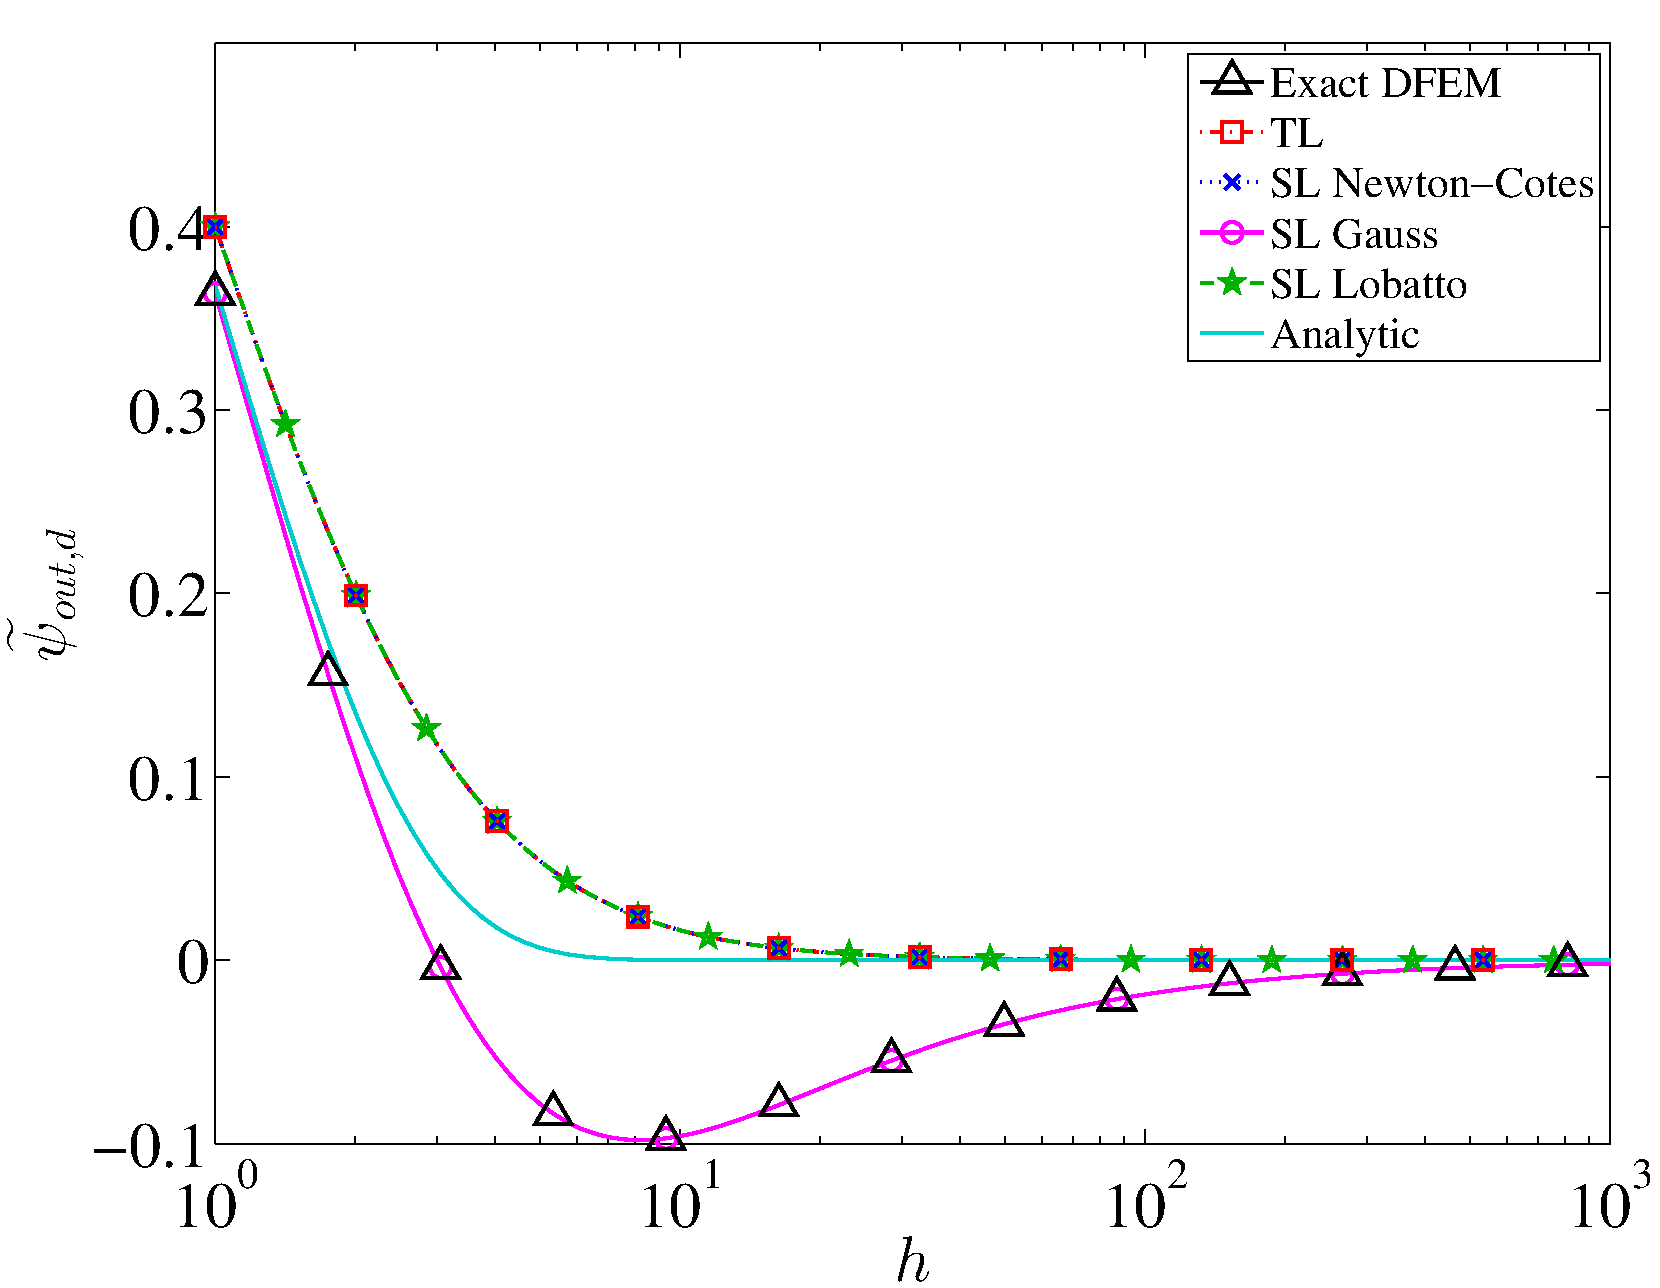
\includegraphics[width=11cm]{chapter2_constant_xs/P1_Outflow_AllMeth-eps-converted-to.pdf}
\caption{Numerical outflow values  as a function of $h$, for a single cell homogeneous absorber problem with a linear DFEM trial space.}
\label{fig:p1_outflow}
\end{figure}
\begin{figure}[!hbp]
\centering
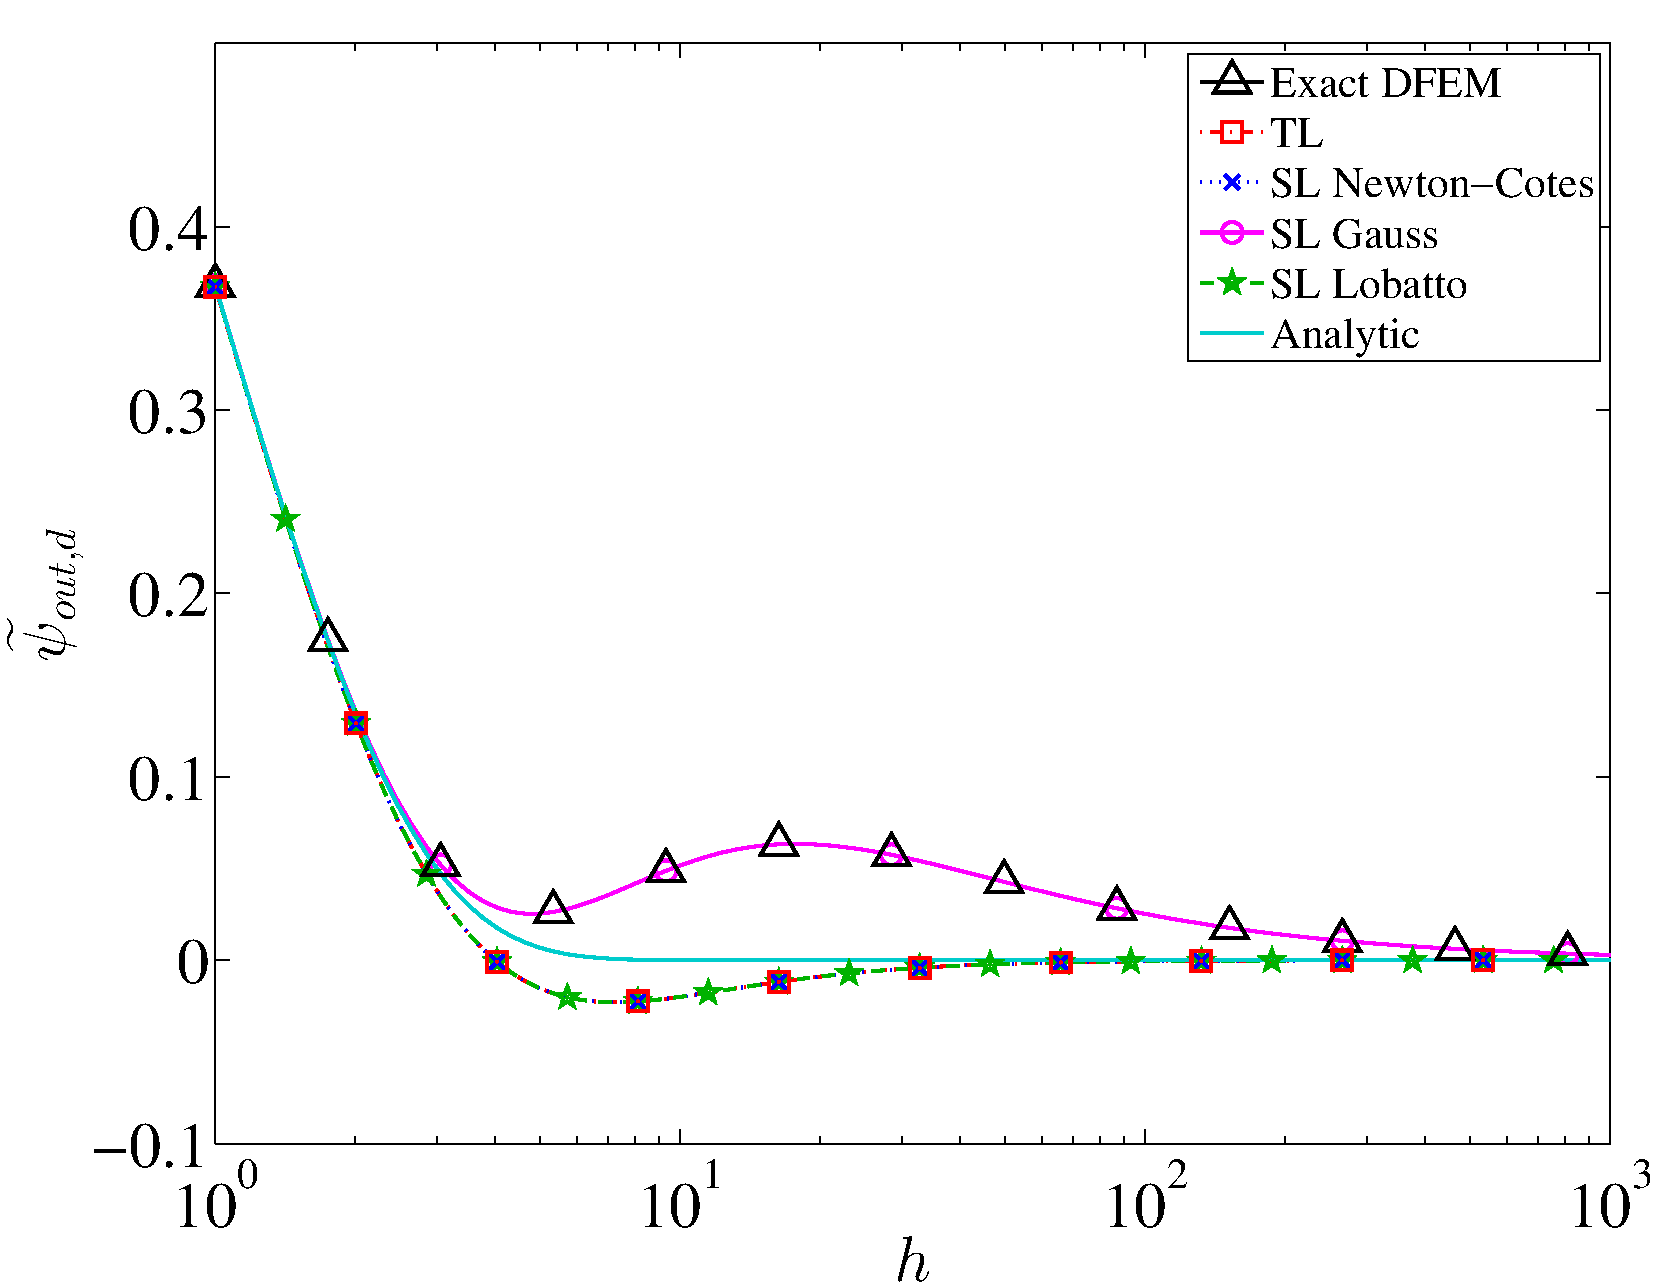
\includegraphics[width=11cm]{chapter2_constant_xs/P2_Outflow_AllMeth-eps-converted-to.pdf}
\caption{Numerical outflow values  as a function of $h$, for a single cell homogeneous absorber problem with a quadratic DFEM trial space.}
\label{fig:p2_outflow}
\end{figure}
\begin{figure}[!htp]
\centering
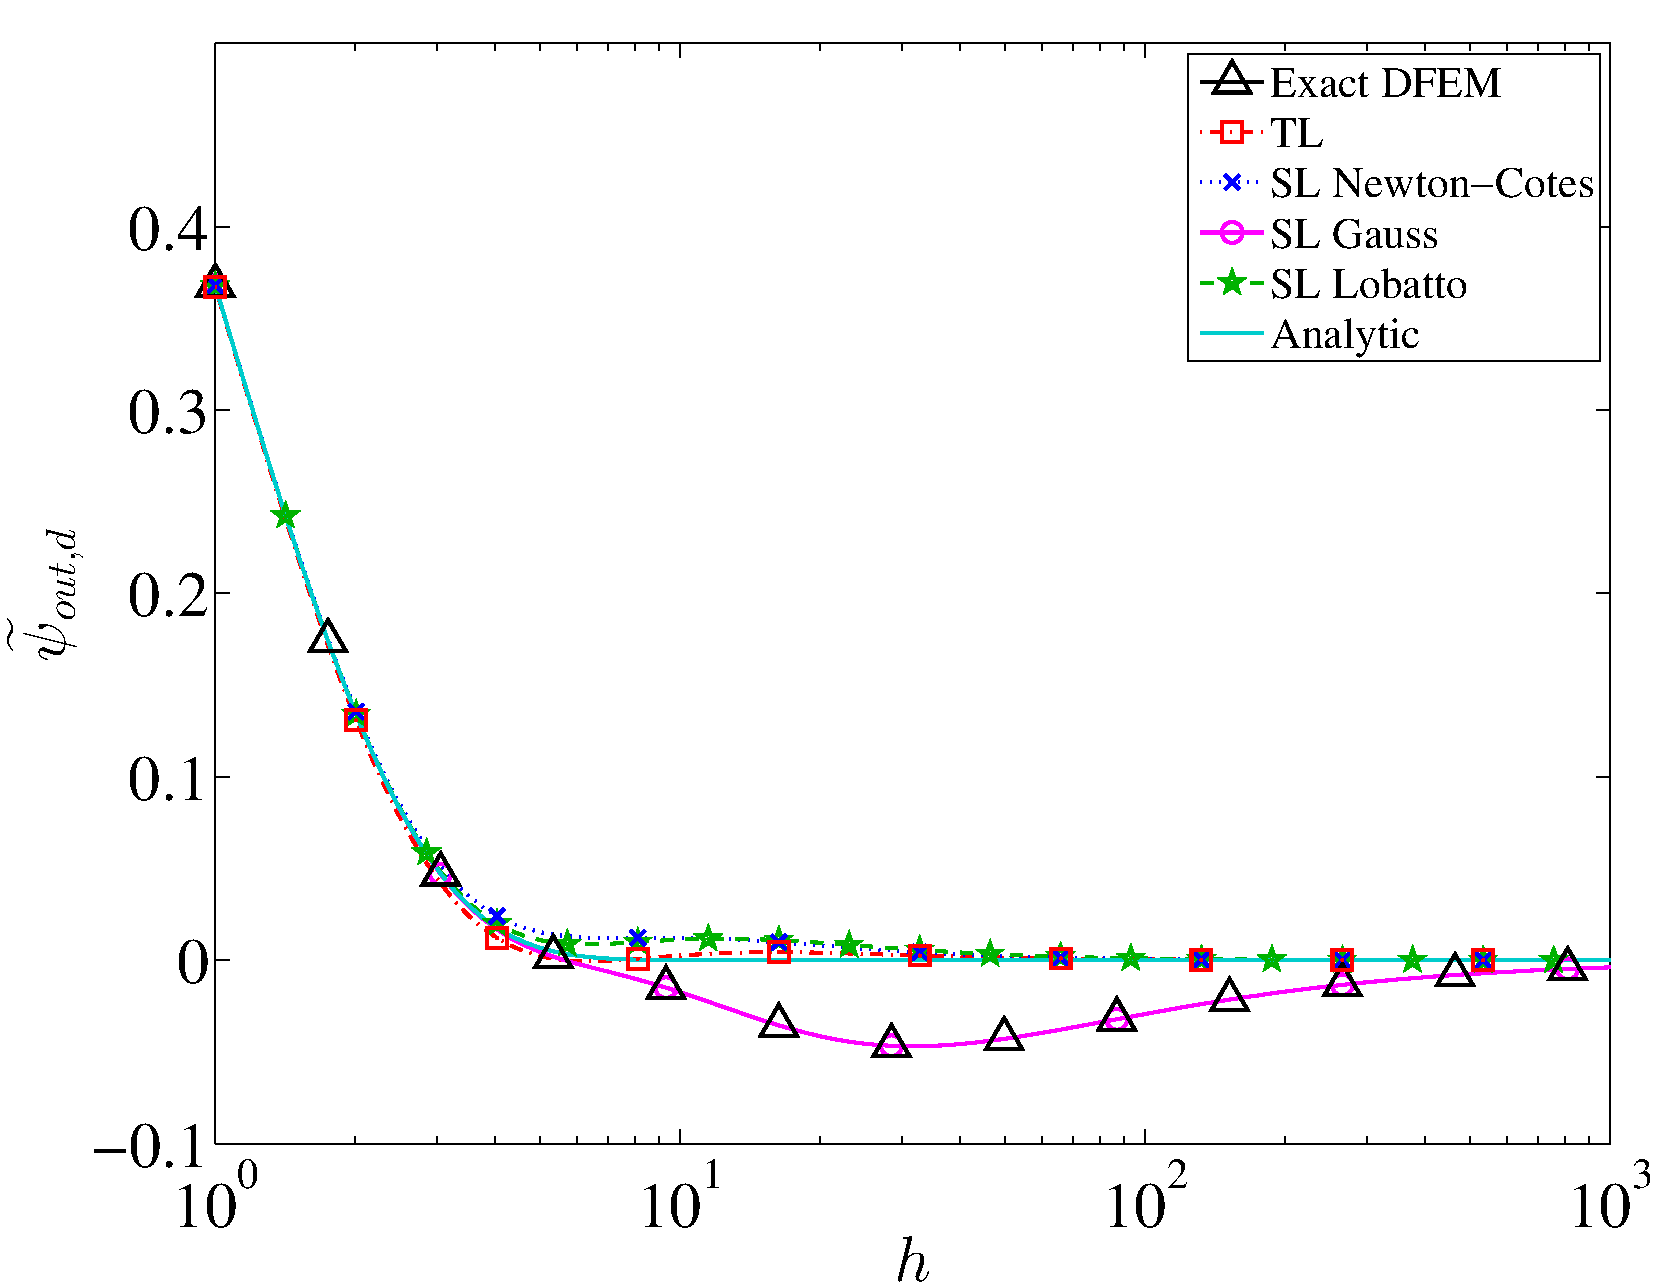
\includegraphics[width=11cm]{chapter2_constant_xs/P3_Outflow_AllMeth-eps-converted-to.pdf}
\caption{Numerical outflow values  as a function of $h$, for a single cell homogeneous absorber problem with a cubic DFEM trial space.}
\label{fig:p3_outflow}
\end{figure}
\begin{figure}[!hbp]
\centering
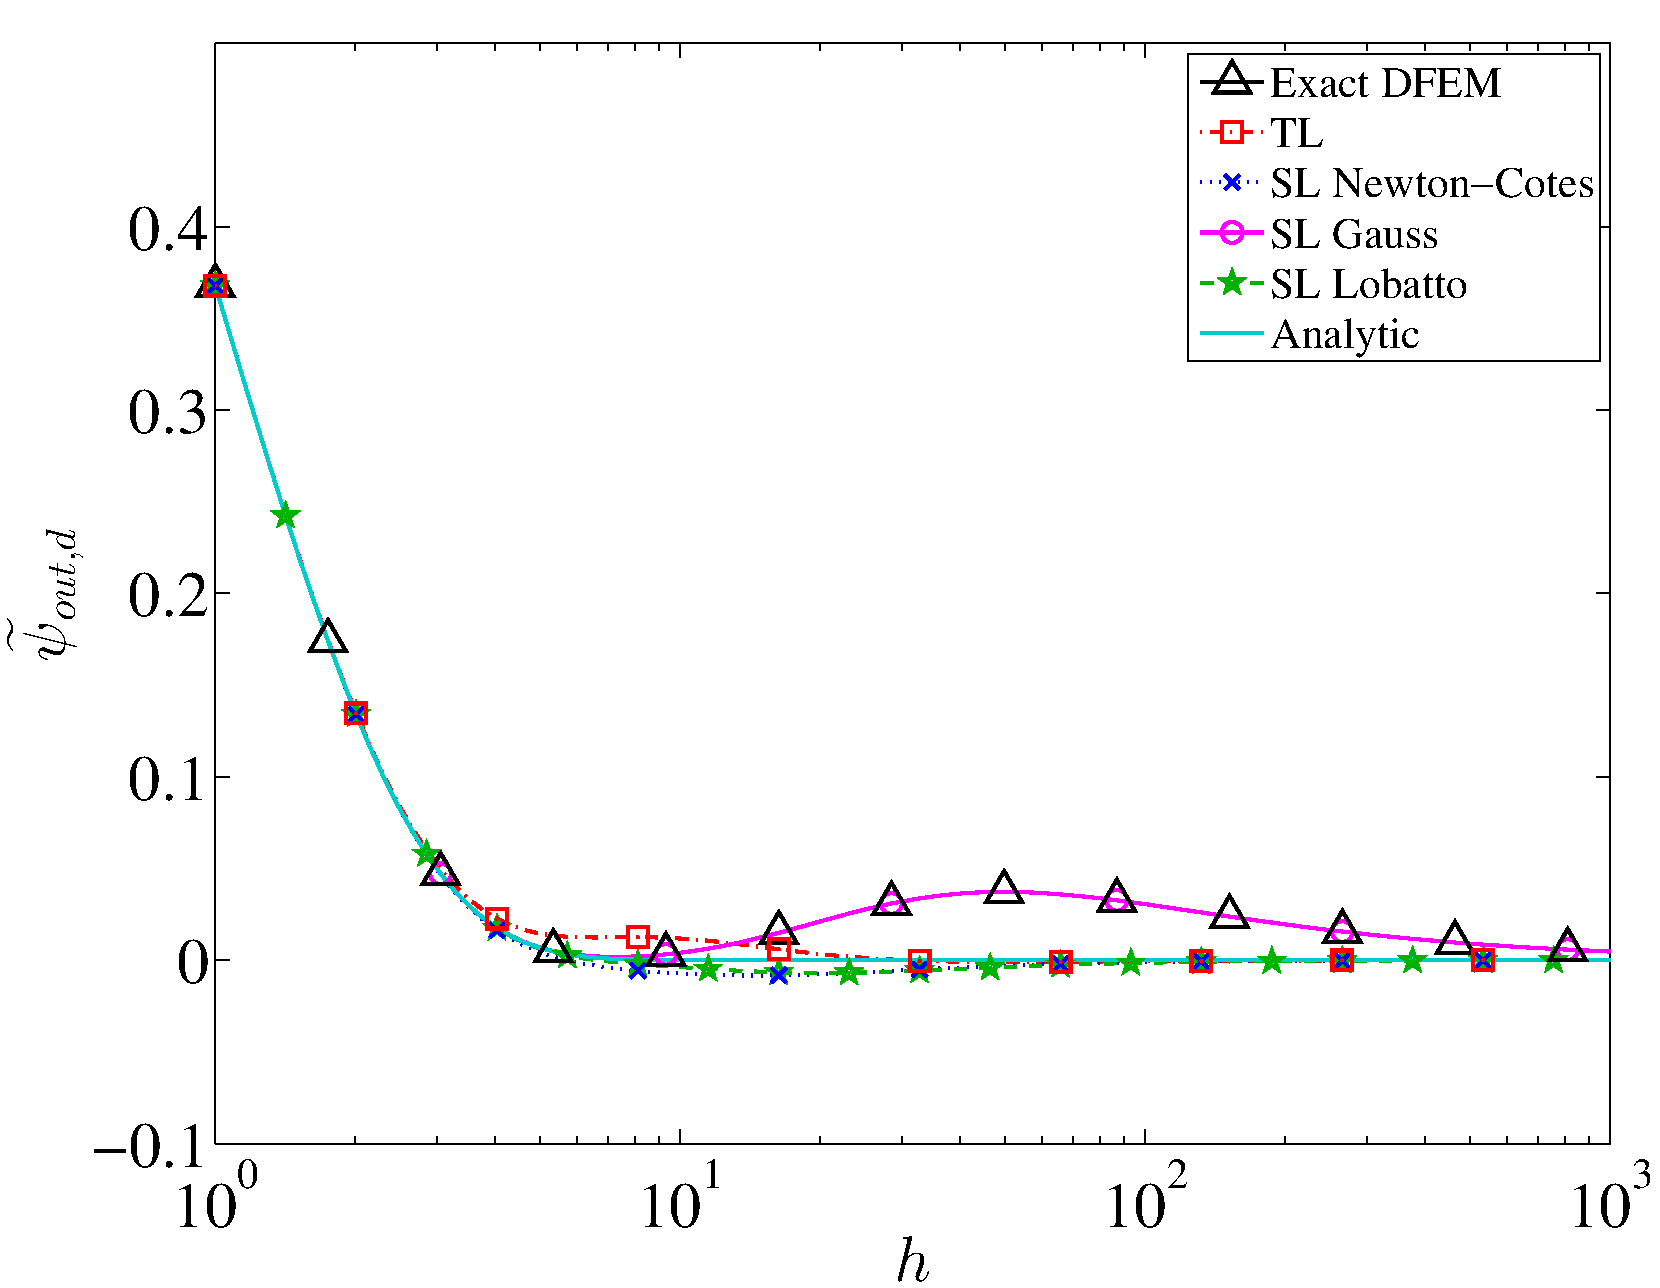
\includegraphics[width=11cm]{chapter2_constant_xs/P4_Outflow_AllMeth-eps-converted-to.pdf}
\caption{Numerical outflow values  as a function of $h$, for a single cell homogeneous absorber problem with a quartic DFEM trial space.}
\label{fig:p4_outflow}
\end{figure}
All methods converge to the analytical solution as $h\to 0$, thus we have zoomed in the range where the methods  visually differ (i.e., $h \ge 1$). 
We observe that:
\begin{itemize}
\item SL Gauss yields strictly positive outflows for even degree polynomial trial spaces,
\item SL Lobatto and SL Newton-Cotes yield strictly positive outflows for odd degree polynomial trial spaces, and
\item TL yields strictly positive outflows only for a linear trial space.
\end{itemize}
We also numerically verify the remarks made of \secref{sec:quad_select}, that is:
\begin{itemize}
\item SL Gauss is equivalent to Exact DFEM,
\item SL Lobatto, SL Newton-Cotes, and TL are equivalent for linear and quadratic trial spaces, and
\item for even degree trial spaces, the outflow value computed by SL Gauss is not monotonically decreasing as a function of $h$ for cells of intermediate optical thickness (the same was noted in \cite{warsa_prinja} for Exact DFEM).
\end{itemize}
%Finally, we note that for even degree polynomial trial spaces, 
%SL Gauss calculates a strictly positive but non-monotonically decreasing value of $\widetilde{\psi}_{out}$ for cells of intermediate optical thickness.
%In addition, Warsa and Prinja also showed that in a source-free pure absorber, a non-physical increase in angular flux outflow occurred in cells of intermediate  optical thickness when using even degree trial spaces.


%%%%%%%%%%%%%%%%%%%%%%%%%%%%%%%%%%%%%%%%%%%%%%%%%%%%%%%%%%%%%%%%%%
\subsection{Fixed Source Single-Cell Inflow Comparison}
\label{sec:inflow}
%%%%%%%%%%%%%%%%%%%%%%%%%%%%%%%%%%%%%%%%%%%%%%%%%%%%%%%%%%%%%%%%%%

As noted in \cite{csz}, it is possible for LDFEM to yield negative solutions near cell inflows for source driven problems.
In this second problem, we use a $\delta$-source:
\benum
Q_d(x) = \left\{ \begin{array}{ll} \delta(x-x_o) & \text{for} ~~ \mu_d > 0 \\ 0  &  \text{for} ~~ \mu_d < 0 \end{array} \right. \pec
\eenum  
$x\in\left[-1,1 \right]$, and $-1 \leq x_o \leq 1$.
The analytic solution to this problem for $\mu_d > 0$ is:
\benum
\psi(x,\mu_d) = \left \{ \begin{array}{ll} \exp\left[-\frac{\Sigma_t(x - x_o)}{\mu_d}  \right] & x \geq x_o \\ 0 & x < x_o \end{array} \right.  \pep
\eenum 
(For $\mu_d < 0$, $\psi(x,\mu_d) = 0$.)
%
We now examine the numerical approximation to the angular flux near the cell inflow, $\widetilde{\psi}_{in,d}$, for various integration 
schemes, trial space degrees, and as a function of the ratio of the first Legendre moment of the source, $S_1$, to the zero-th Legendre moment of the source, $S_0$.
Note that the physical range of that ratio, $\frac{S_1}{S_0}$, is $[-3,3]$, corresponding to a $\delta$-source at the left cell edge $(\frac{S_1}{S_0} = -3)$ or at the right edge $(\frac{S_1}{S_0} = 3)$.

We first consider the case of a vacuum ($\Sigma_t=0$), thus only testing the effect of quadrature accuracy in evaluating $\vec{Q}_d$ and $\mathbf{G}$.  
In \figs{fig:vac_inflow_p1}{fig:vac_inflow_p4}, we plot $\widetilde{\psi}_{in,d}$ for three schemes:
\begin{enumerate}
\item Lobatto quadrature, which is exact for $\mathbf{G}$ and approximate for the source moments, \eqt{eq:mod_source_moment} ,
\item Gauss quadrature: which is exact for both $\mathbf{G}$ and the source moments, and 
\item Newton-Cotes quadrature: which is approximate for both $\mathbf{G}$ and the source moments.
\end{enumerate}
\begin{figure}[!hbp]
\centering
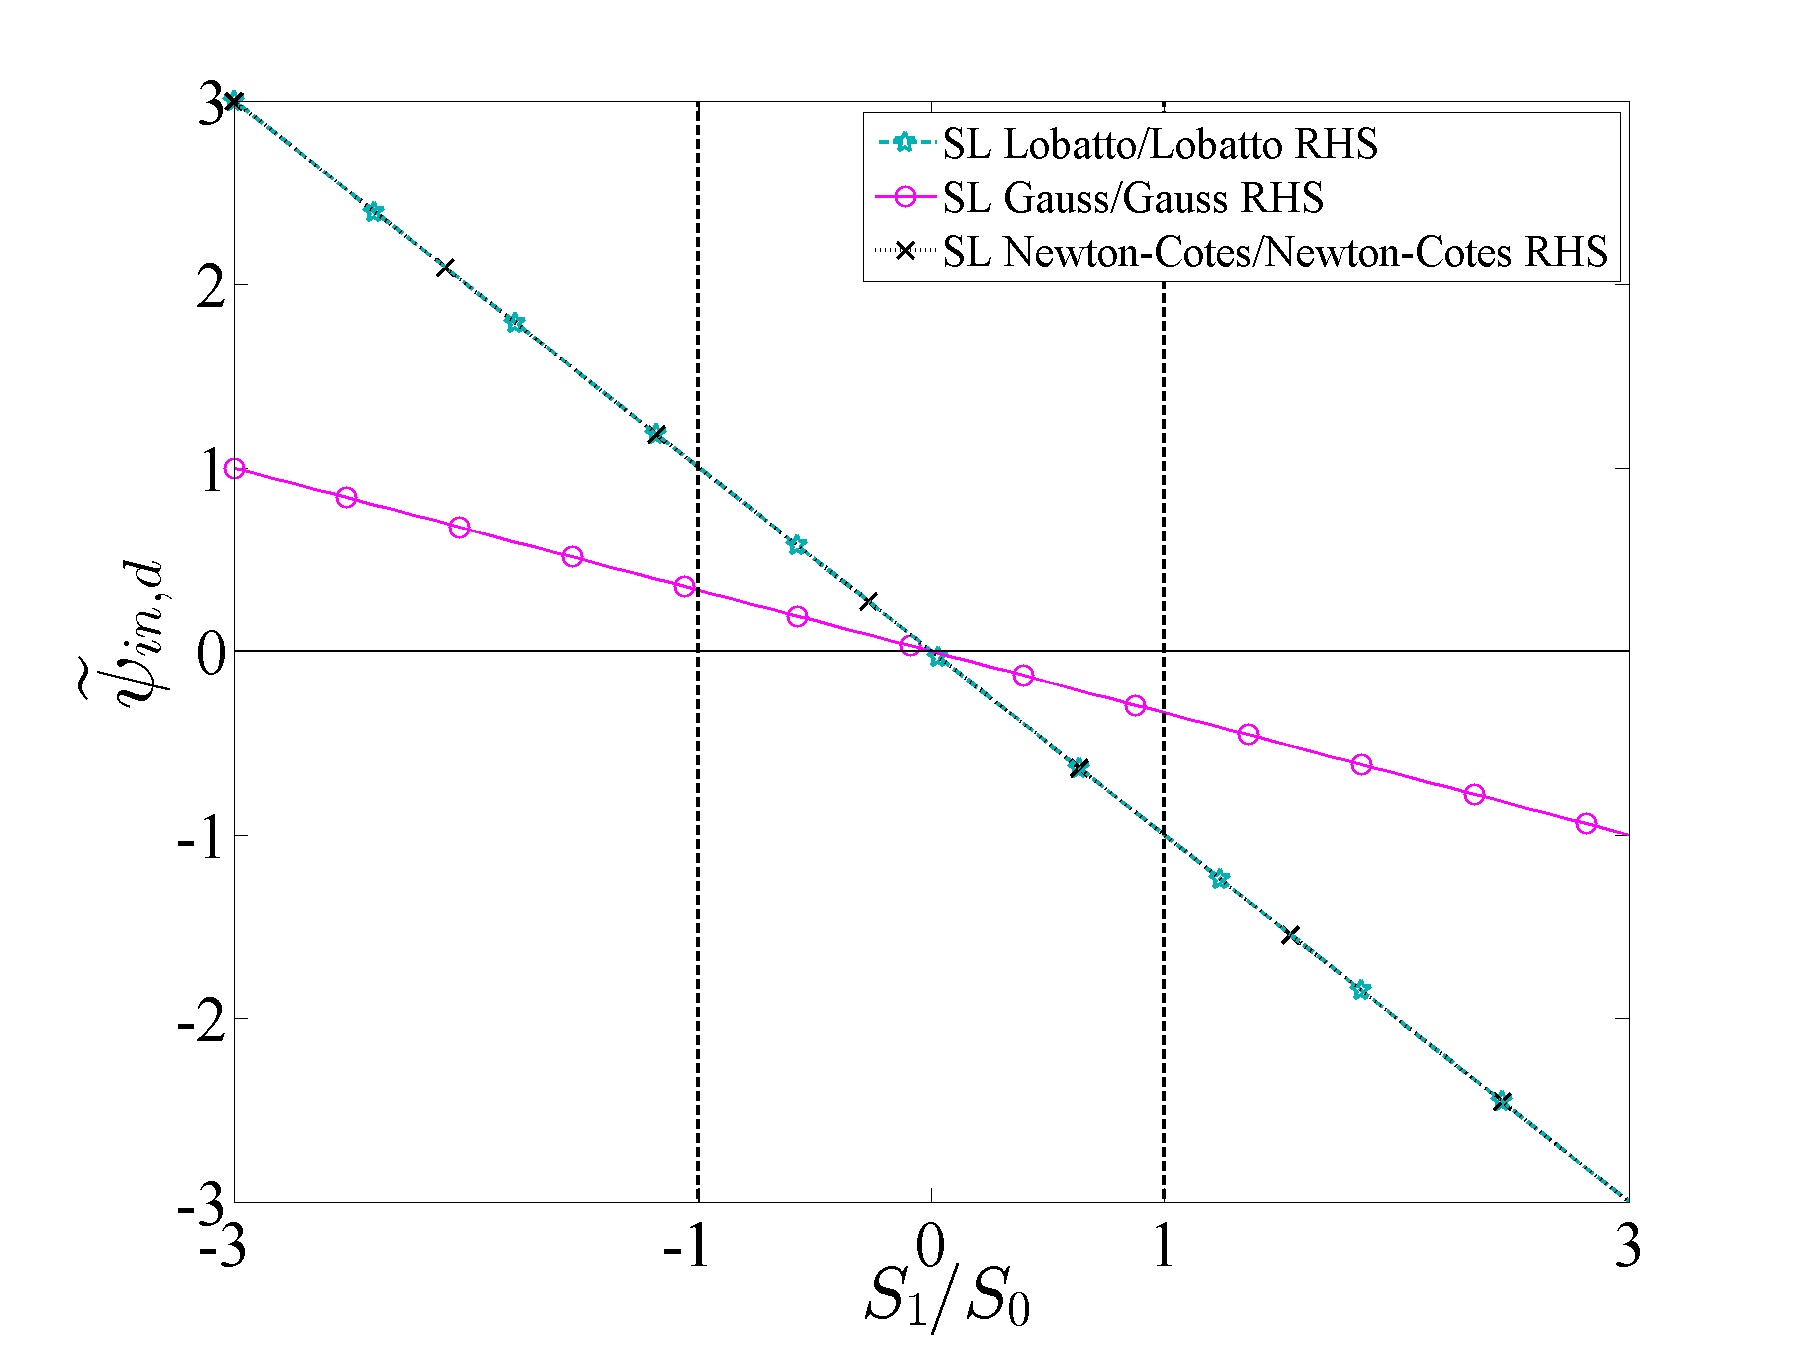
\includegraphics[width=11cm]{chapter2_constant_xs/Final_Inflow_RHS_Comparison_Source_P1_MFP_0.png}
\caption{Numerical inflow values as a function of $\frac{S_1}{S_0}$ for a single cell (vacuum case) with a $\delta$-shaped source, using linear DFEM.}
\label{fig:vac_inflow_p1}
\end{figure}
\begin{figure}[!htp]
\centering
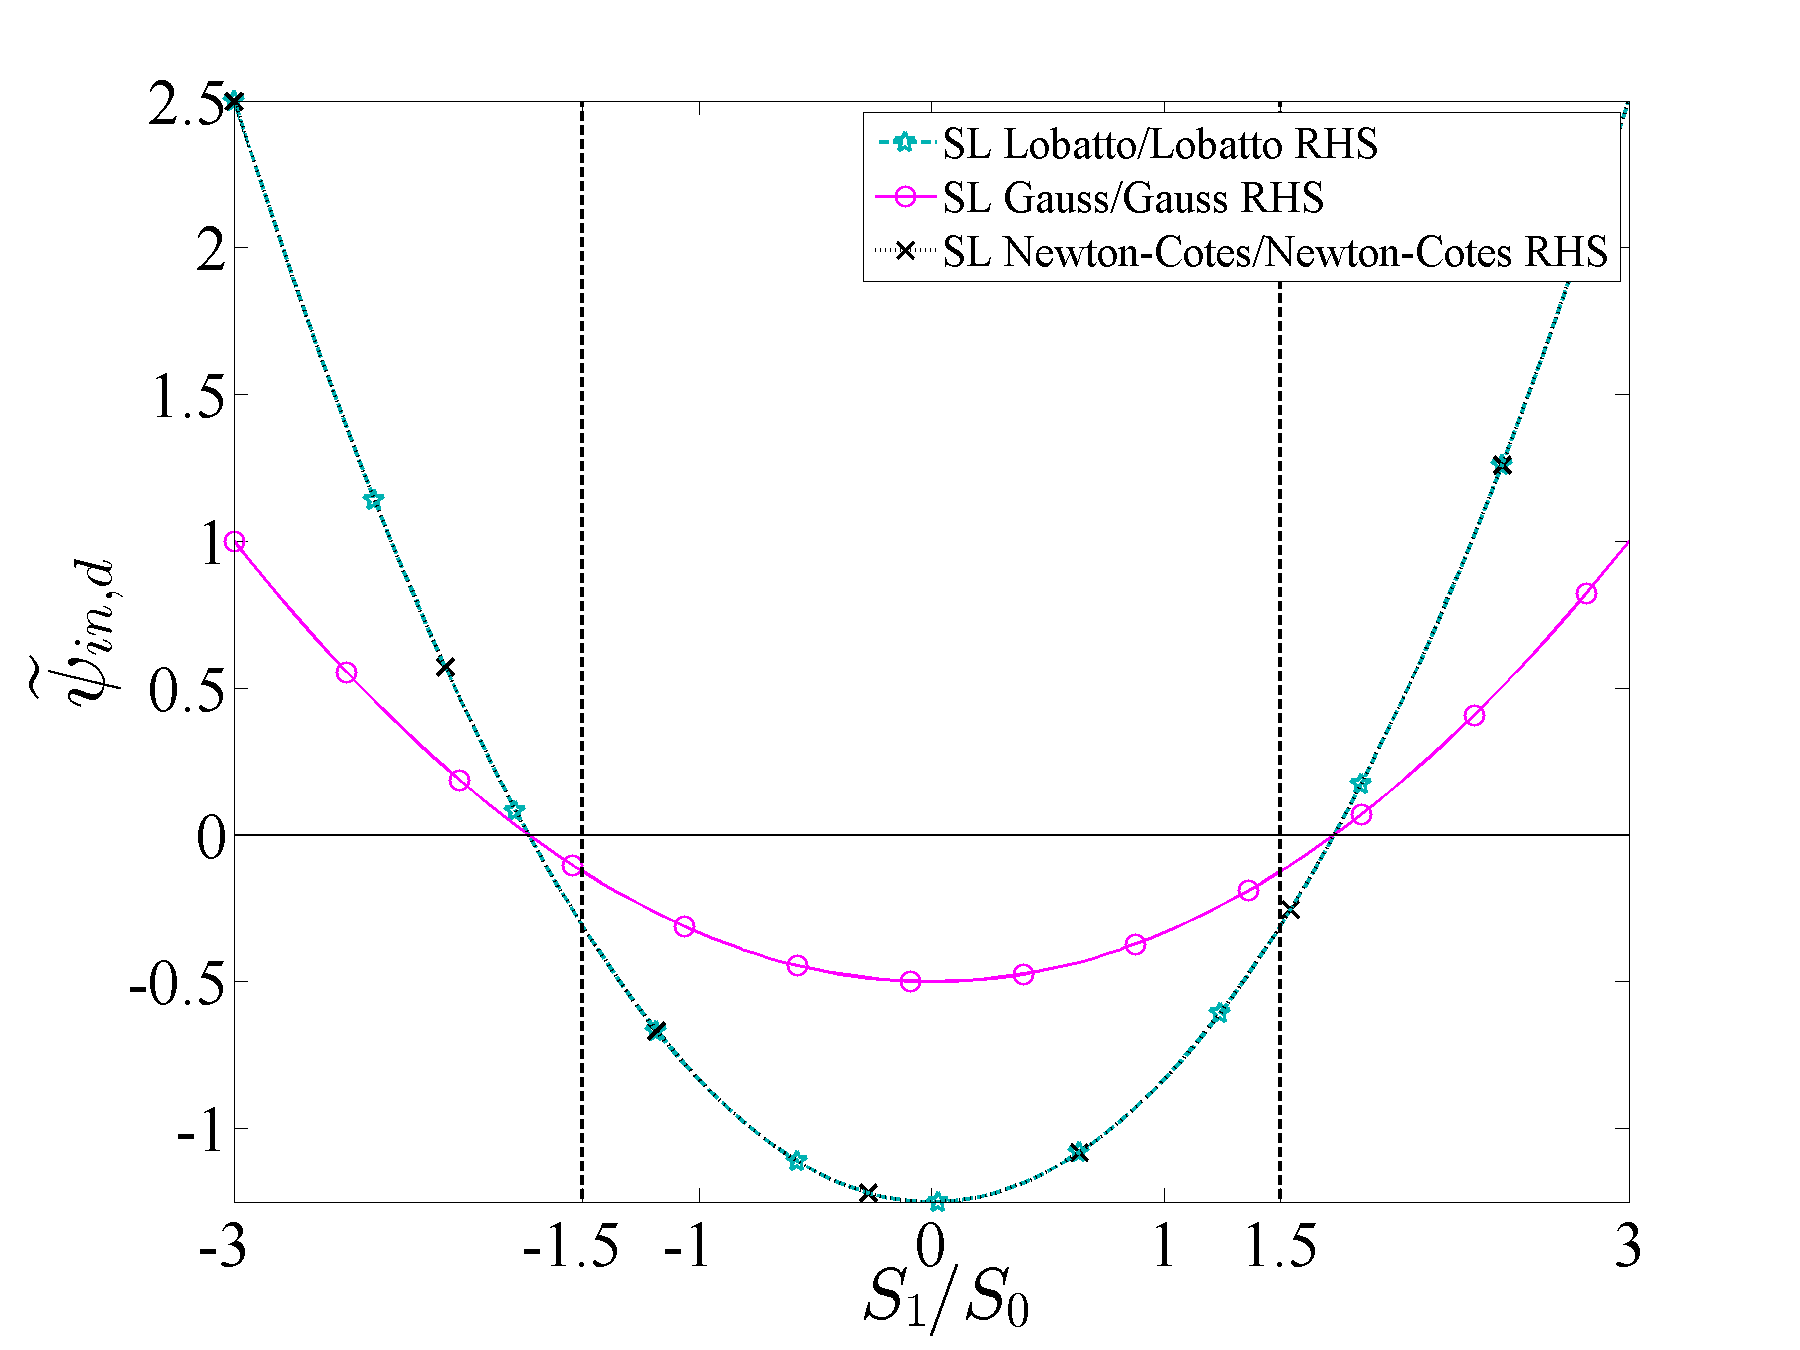
\includegraphics[width=11cm]{chapter2_constant_xs/Final_Inflow_RHS_Comparison_Source_P2_MFP_0.png}
\caption{Numerical inflow values as a function of $\frac{S_1}{S_0}$ for a single cell (vacuum case) with a $\delta$-shaped source, using quadratic DFEM.}
\label{fig:vac_inflow_p2}
\end{figure}
\begin{figure}[!hbp]
\centering
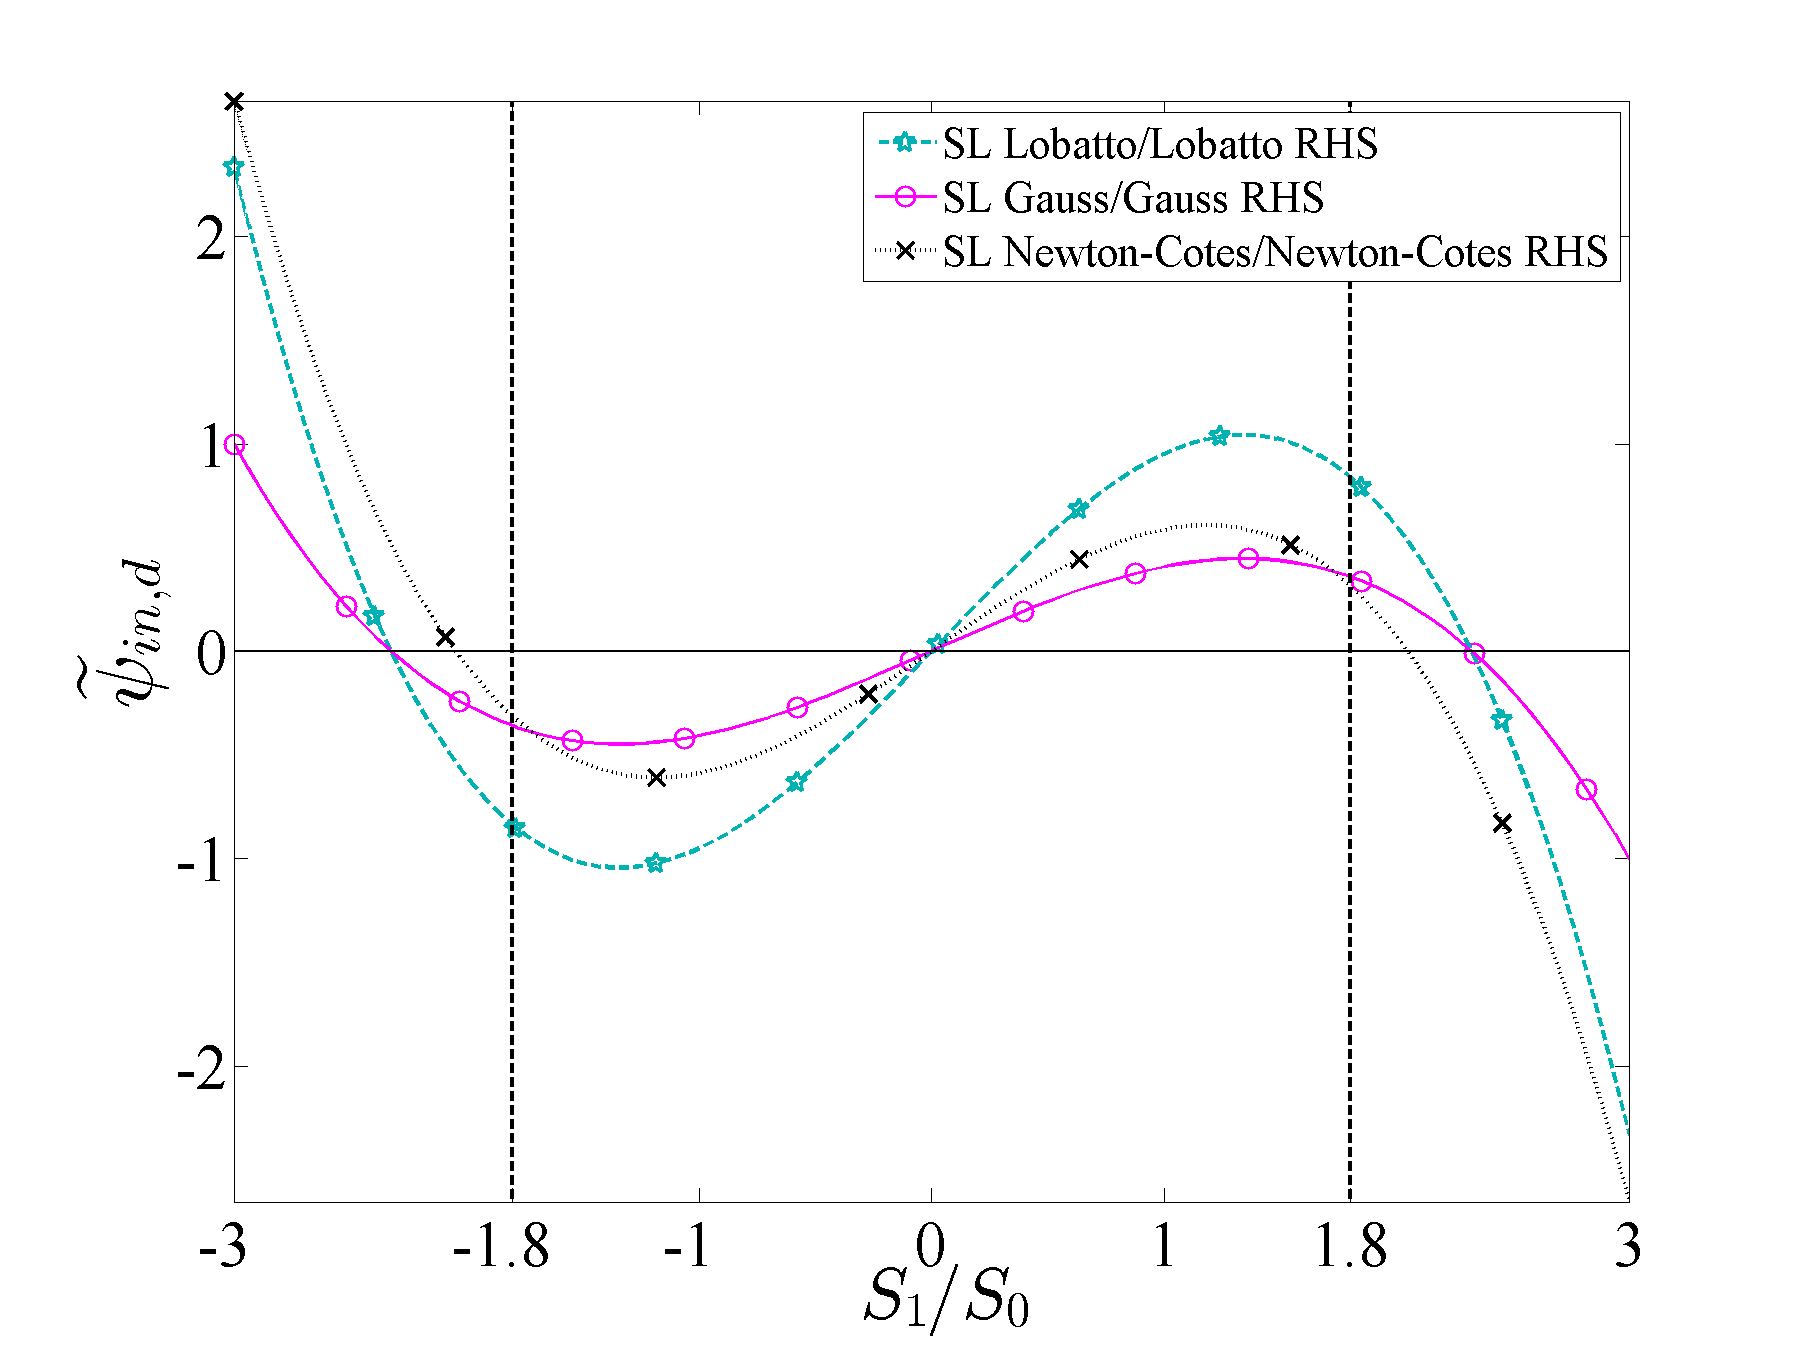
\includegraphics[width=11cm]{chapter2_constant_xs/Final_Inflow_RHS_Comparison_Source_P3_MFP_0.png}
\caption{Numerical inflow values as a function of $\frac{S_1}{S_0}$ for a single cell (vacuum case) with a $\delta$-shaped source, using cubic DFEM.}
\label{fig:vac_inflow_p3}
\end{figure}
\begin{figure}[!htp]
\centering
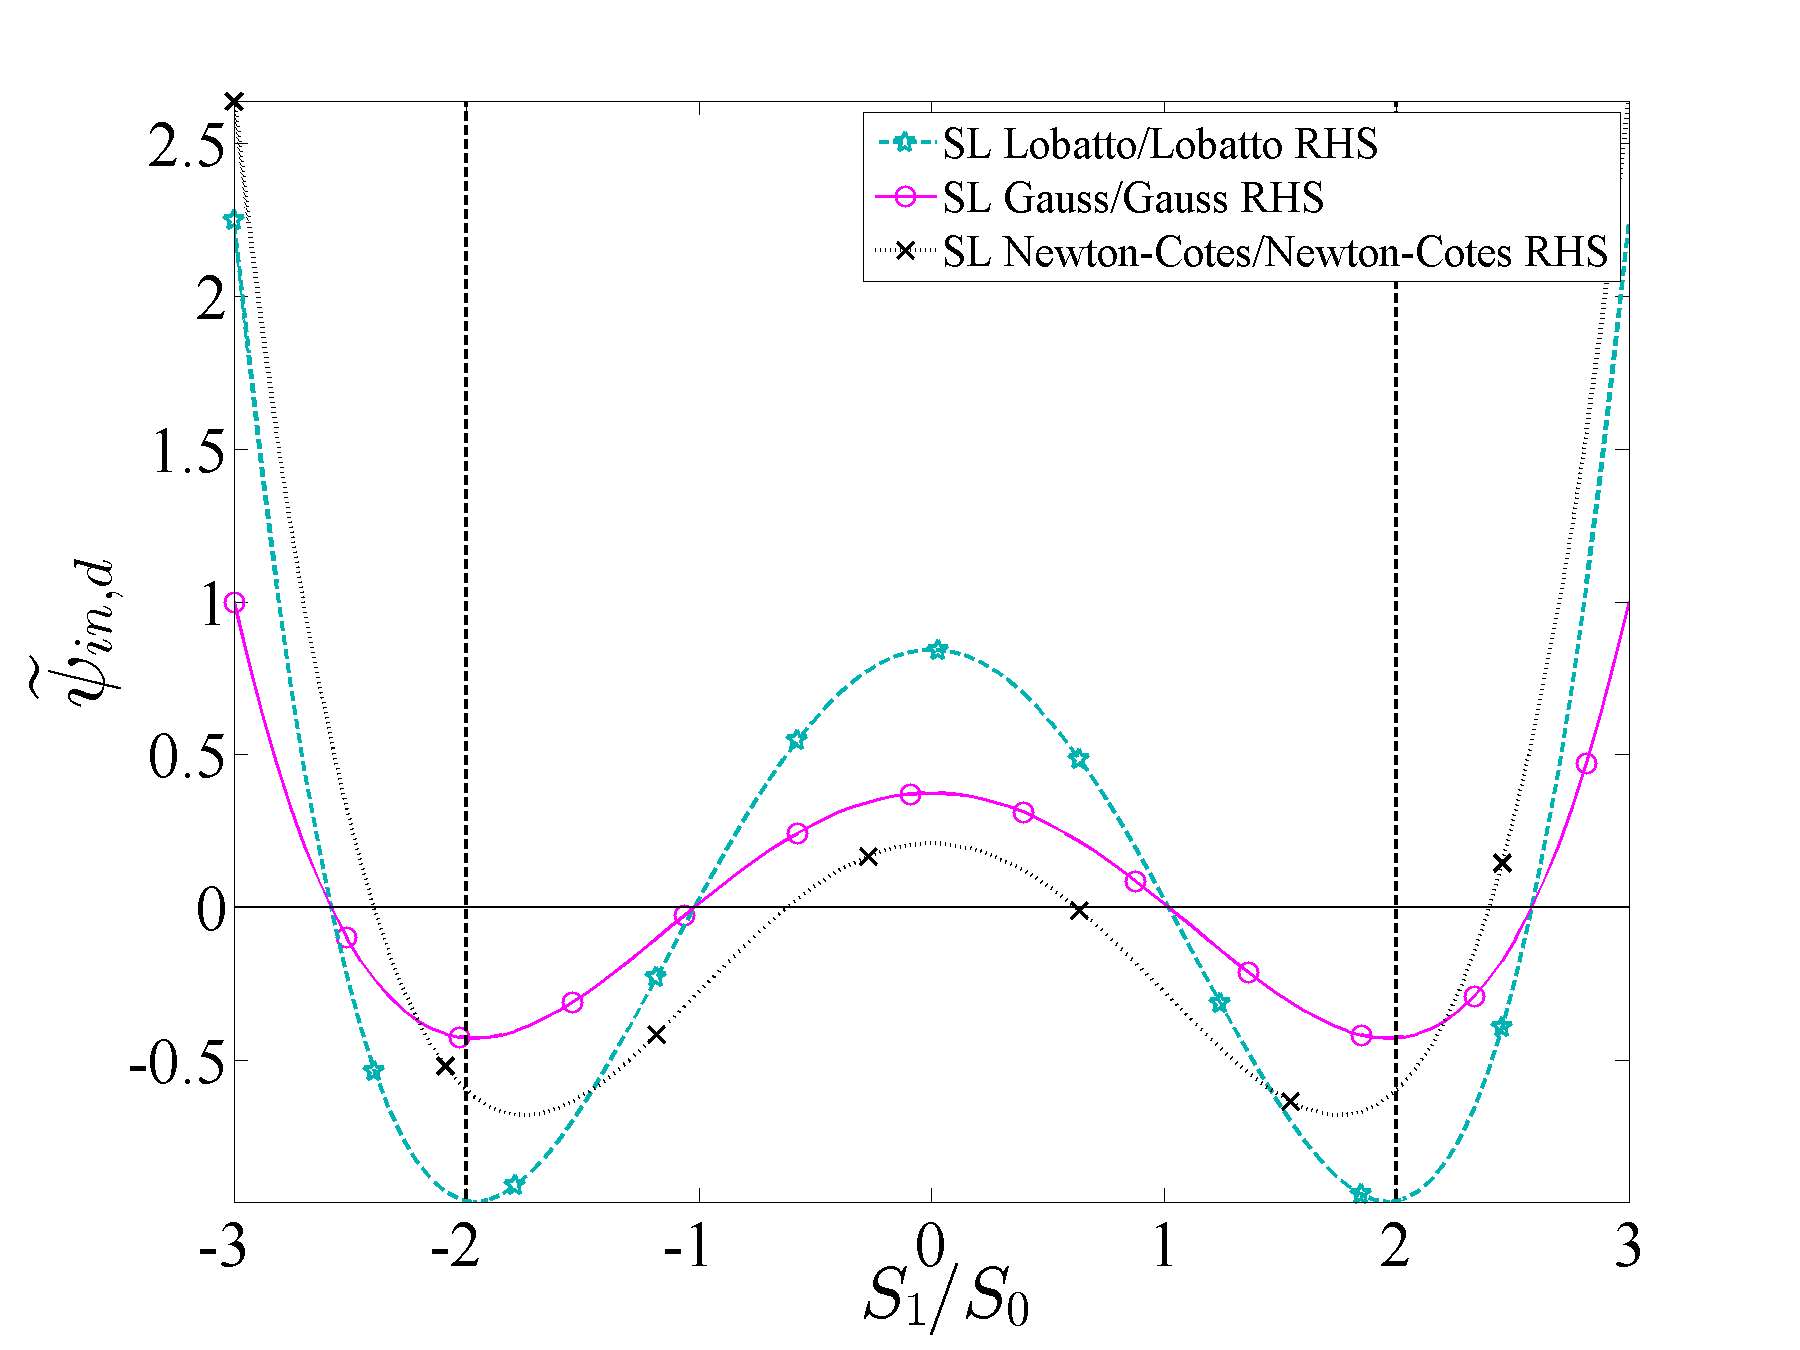
\includegraphics[width=11cm]{chapter2_constant_xs/Final_Inflow_RHS_Comparison_Source_P4_MFP_0.png}
\caption{Numerical inflow values as a function of $\frac{S_1}{S_0}$ for a single cell (vacuum case) with a $\delta$-shaped source, using quartic DFEM.}
\label{fig:vac_inflow_p4}
\end{figure}

The dotted vertical lines in \figs{fig:vac_inflow_p1}{fig:vac_inflow_p4} correspond to the extrema values of $\frac{S_1}{S_0}$ that yield a strictly positive polynomial source representation of degree $P$ 
(indeed, the degree-$P$ Legendre expansion of the $\delta$-source is not everywhere positive for a wide range of possible $\frac{S_1}{S_0}$ that are physically realizable).
For all trial space degrees, the Gauss scheme exhibits less negativity than either of the other two schemes.
The dramatic difference between the Gauss scheme and the Lobatto scheme is solely due to the quadrature formula used to evaluate $\vec{Q}_d$ since both schemes exactly integrate $\mathbf{G}$.
The Newton-Cotes scheme exhibits less severe negativities than the Lobatto scheme but is less robust than the Gauss scheme.
Given the results shown in \figs{fig:vac_inflow_p1}{fig:vac_inflow_p4}, we conclude that the most robust schemes exactly integrate the source moments, \eqt{eq:mod_source_moment}.

\begin{figure}[!htp]
\centering
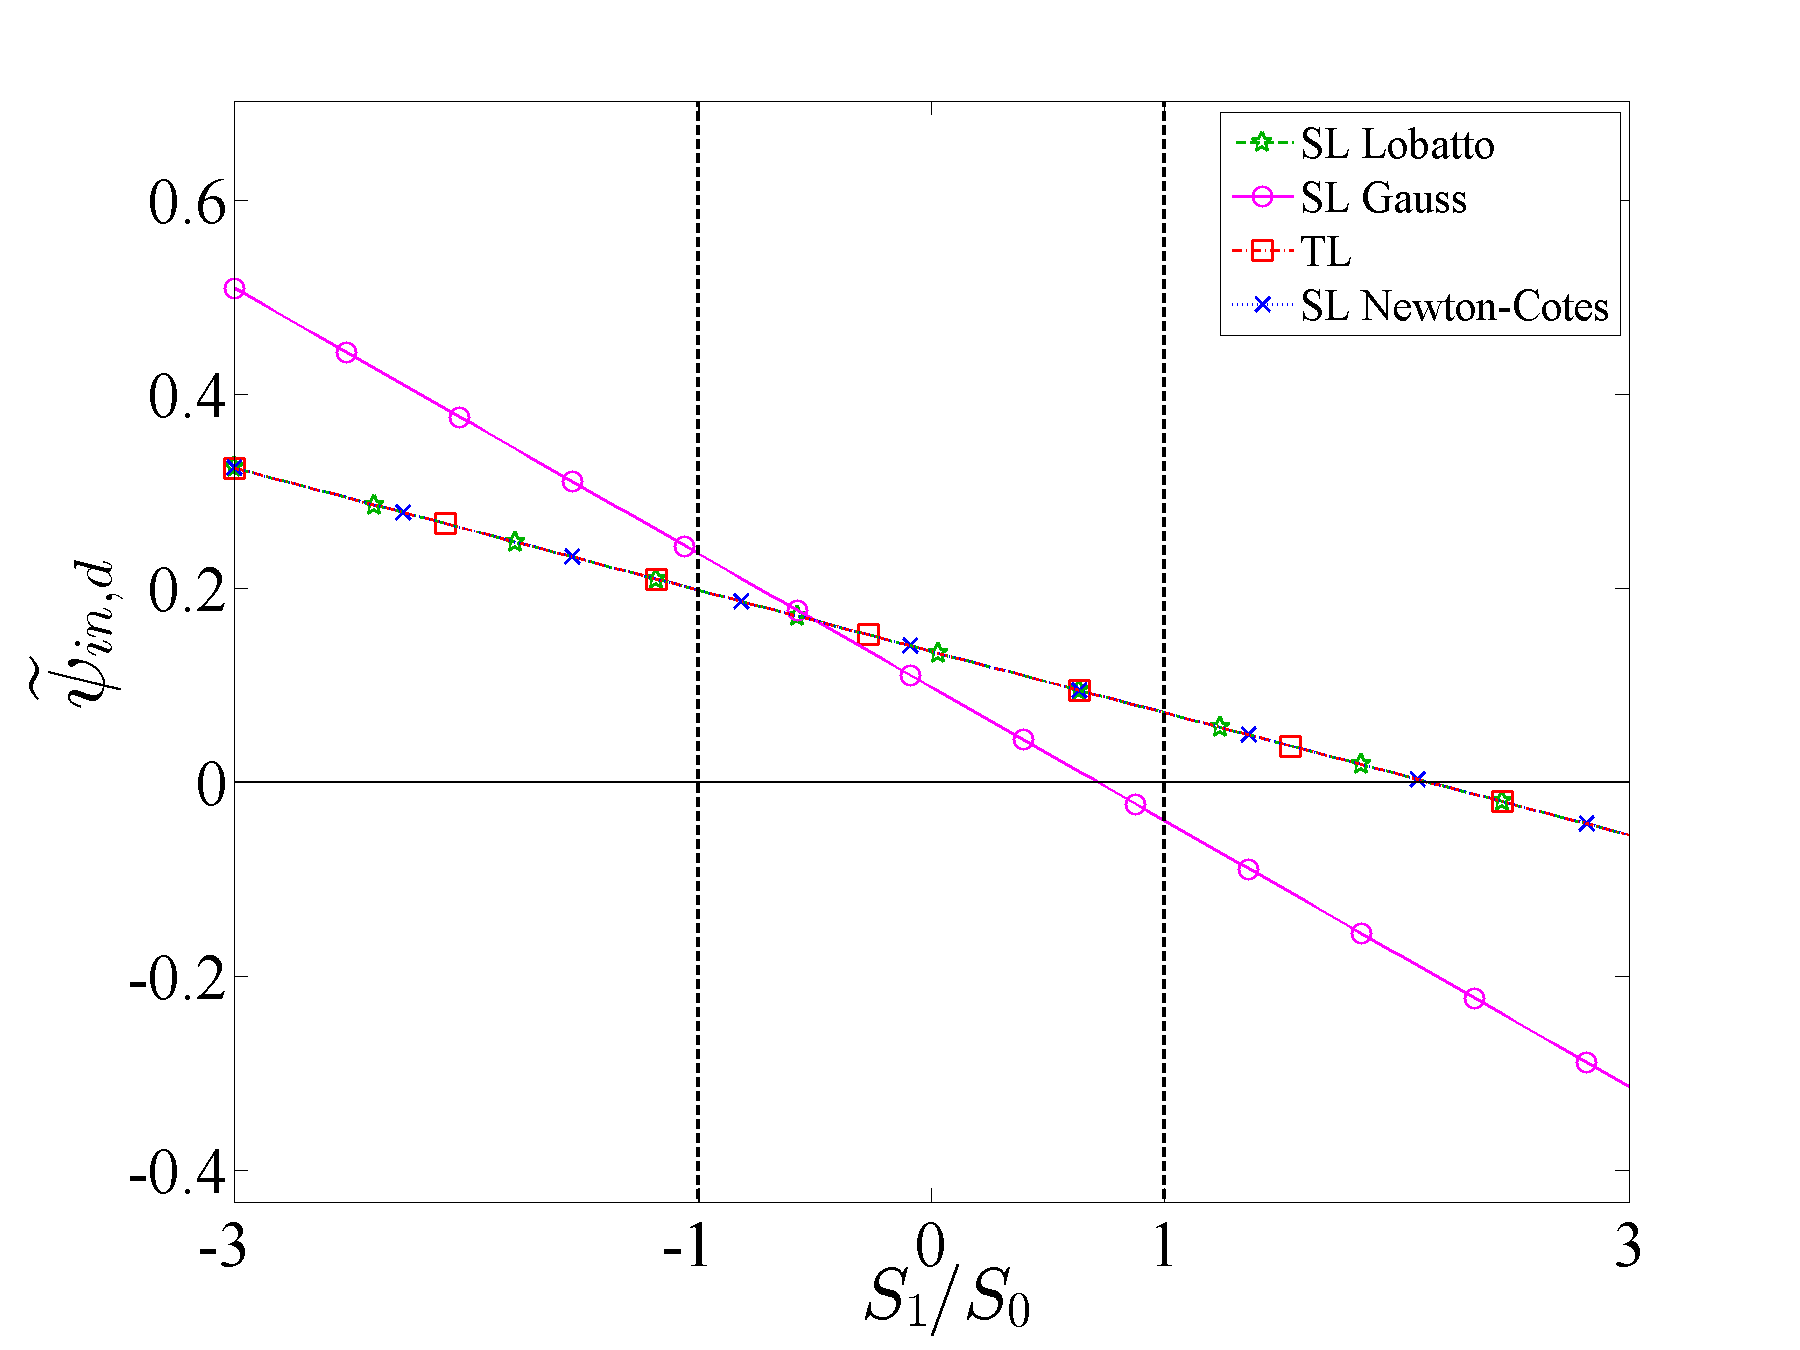
\includegraphics[width=11cm]{chapter2_constant_xs/Final_Inflow_RHS_Comparison_Source_P1_MFP_5.png}
\caption{Numerical inflow values  as a function of $\frac{S_1}{S_0}$, for a single cell (absorber case) with a $\delta$-shaped source, using linear DFEM.}
\label{fig:abs_inflow_p1}
\end{figure}
\begin{figure}[!hbp]
\centering
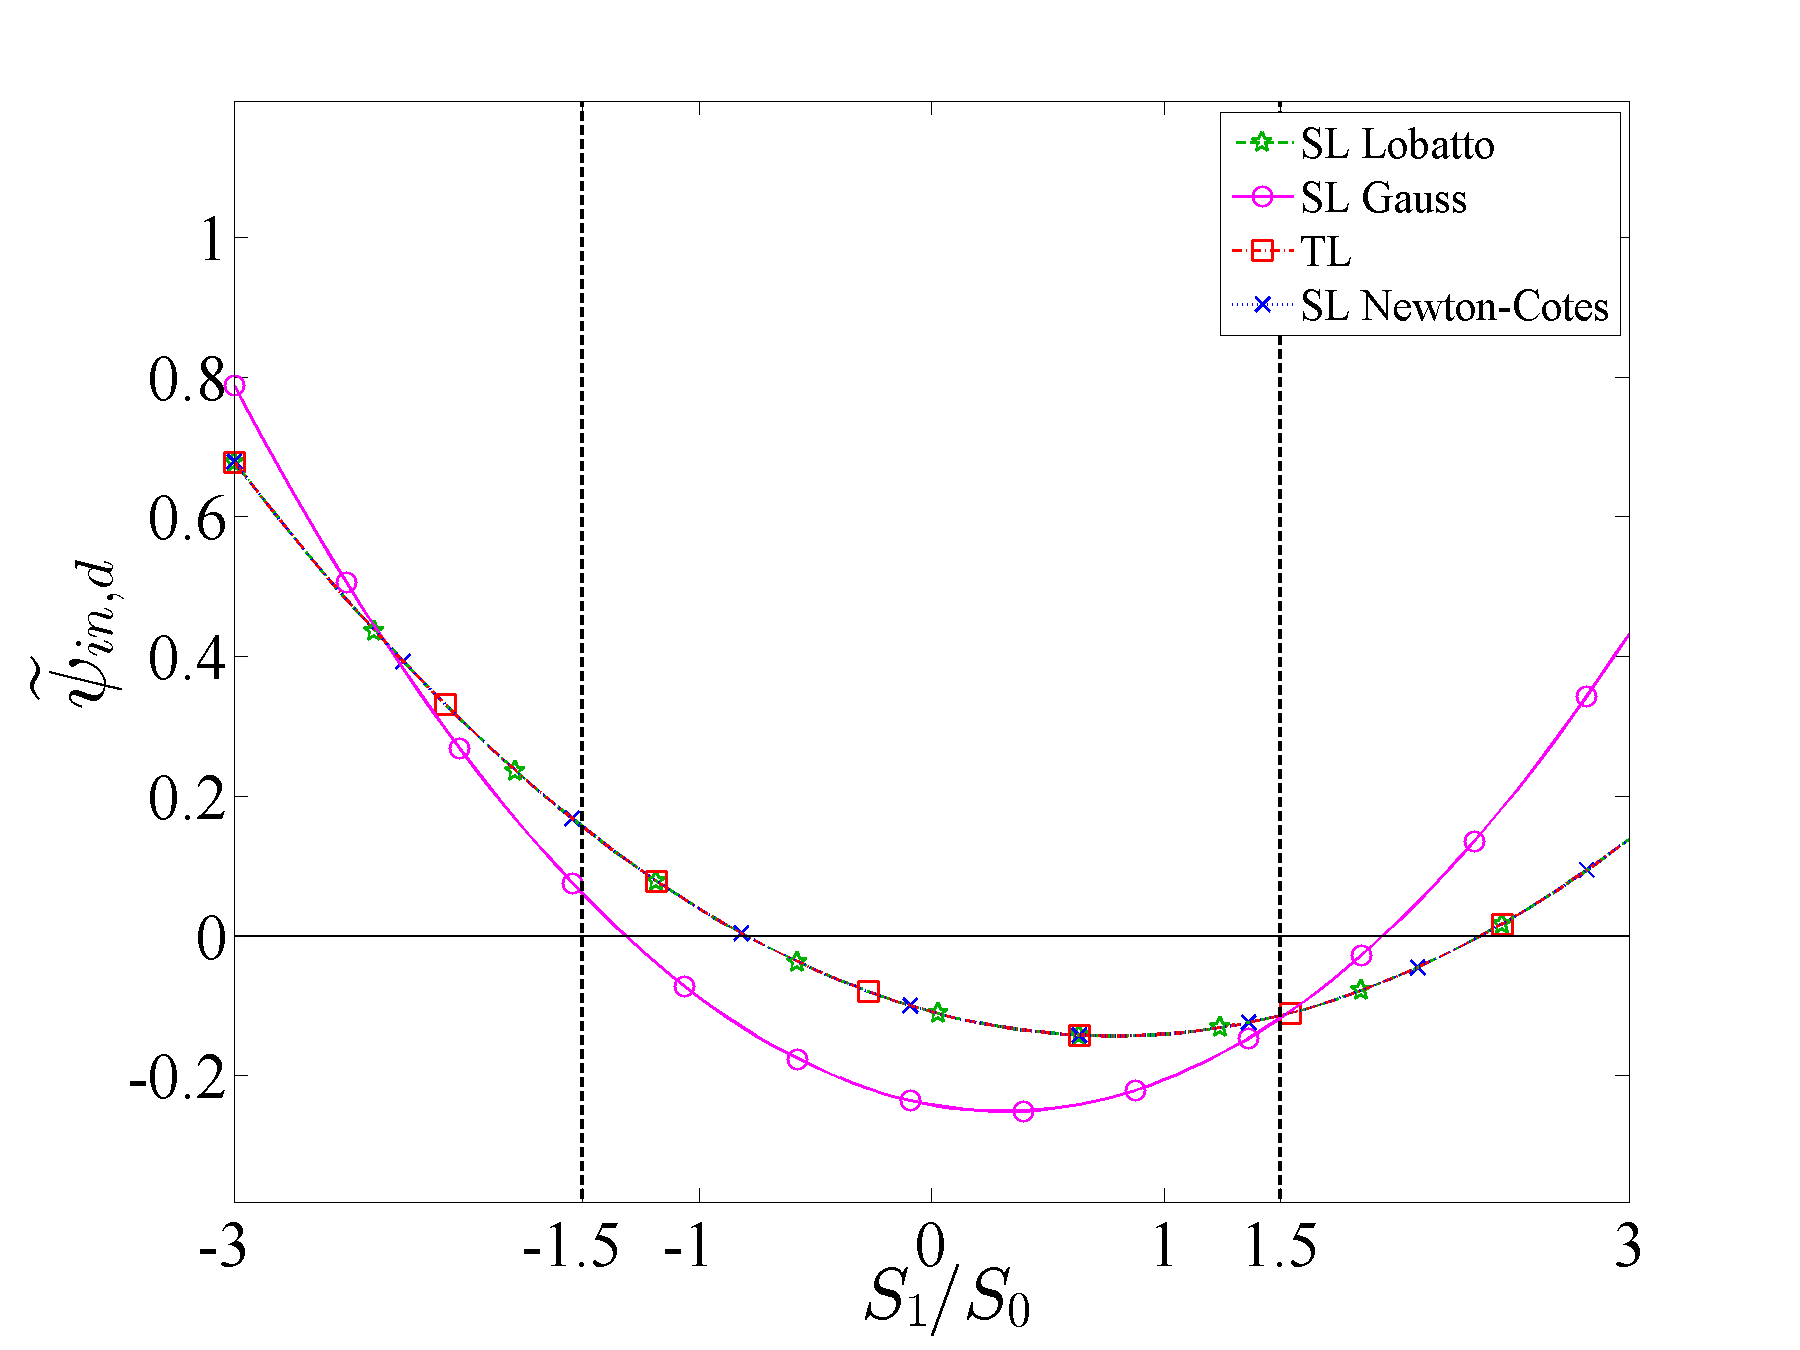
\includegraphics[width=11cm]{chapter2_constant_xs/Final_Inflow_RHS_Comparison_Source_P2_MFP_5.png}
\caption{Numerical inflow values  as a function of $\frac{S_1}{S_0}$, for a single cell (absorber case) with a $\delta$-shaped source, using quadratic DFEM.}
\label{fig:abs_inflow_p2}
\end{figure}
\begin{figure}[!hbp]
\centering
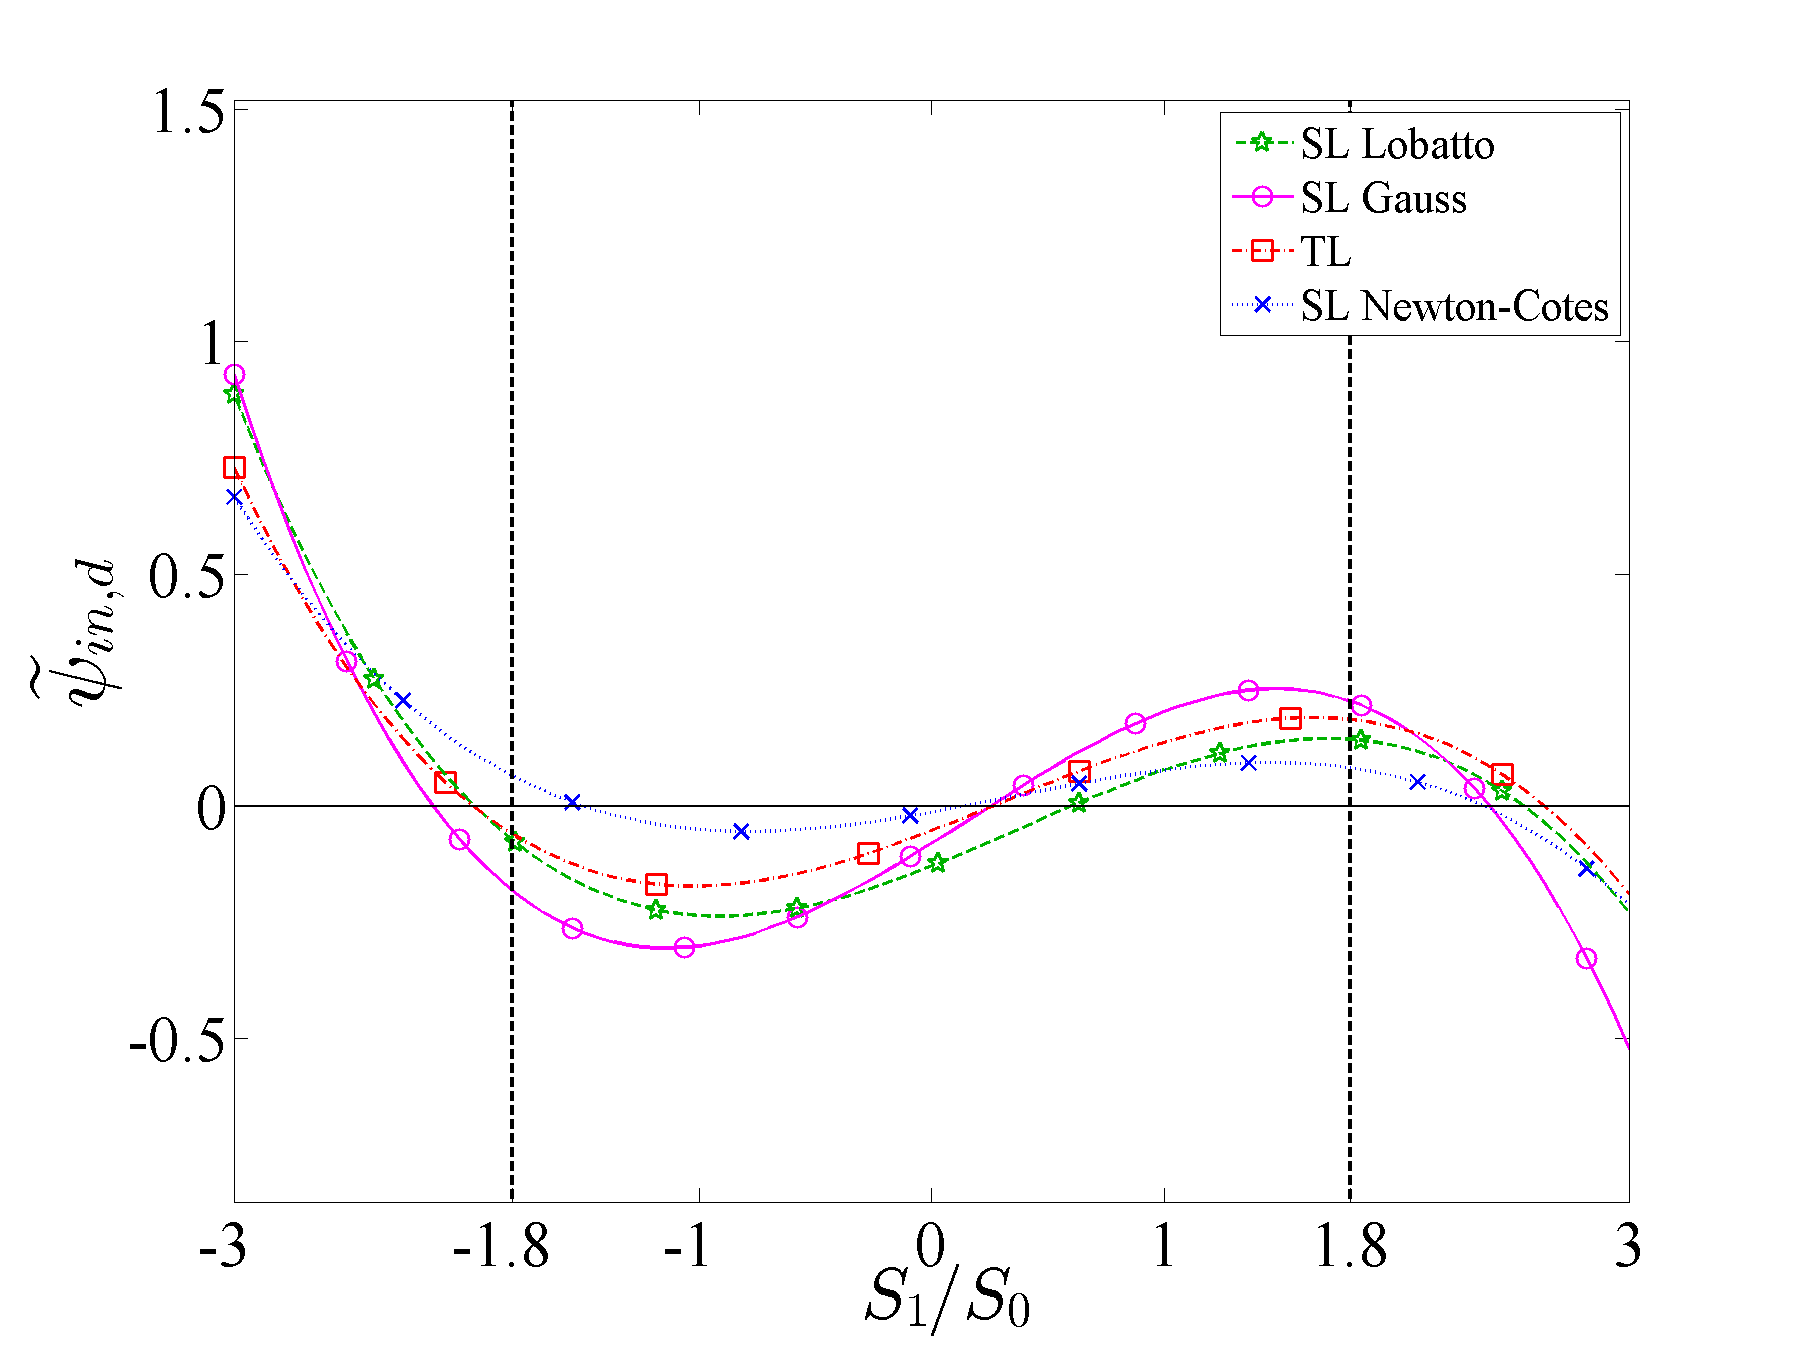
\includegraphics[width=11cm]{chapter2_constant_xs/Final_Inflow_RHS_Comparison_Source_P3_MFP_5.png}
\caption{Numerical inflow values  as a function of $\frac{S_1}{S_0}$, for a single cell (absorber case) with a $\delta$-shaped source, using cubic DFEM.}
\label{fig:abs_inflow_p3}
\end{figure}
\begin{figure}[!htp]
\centering
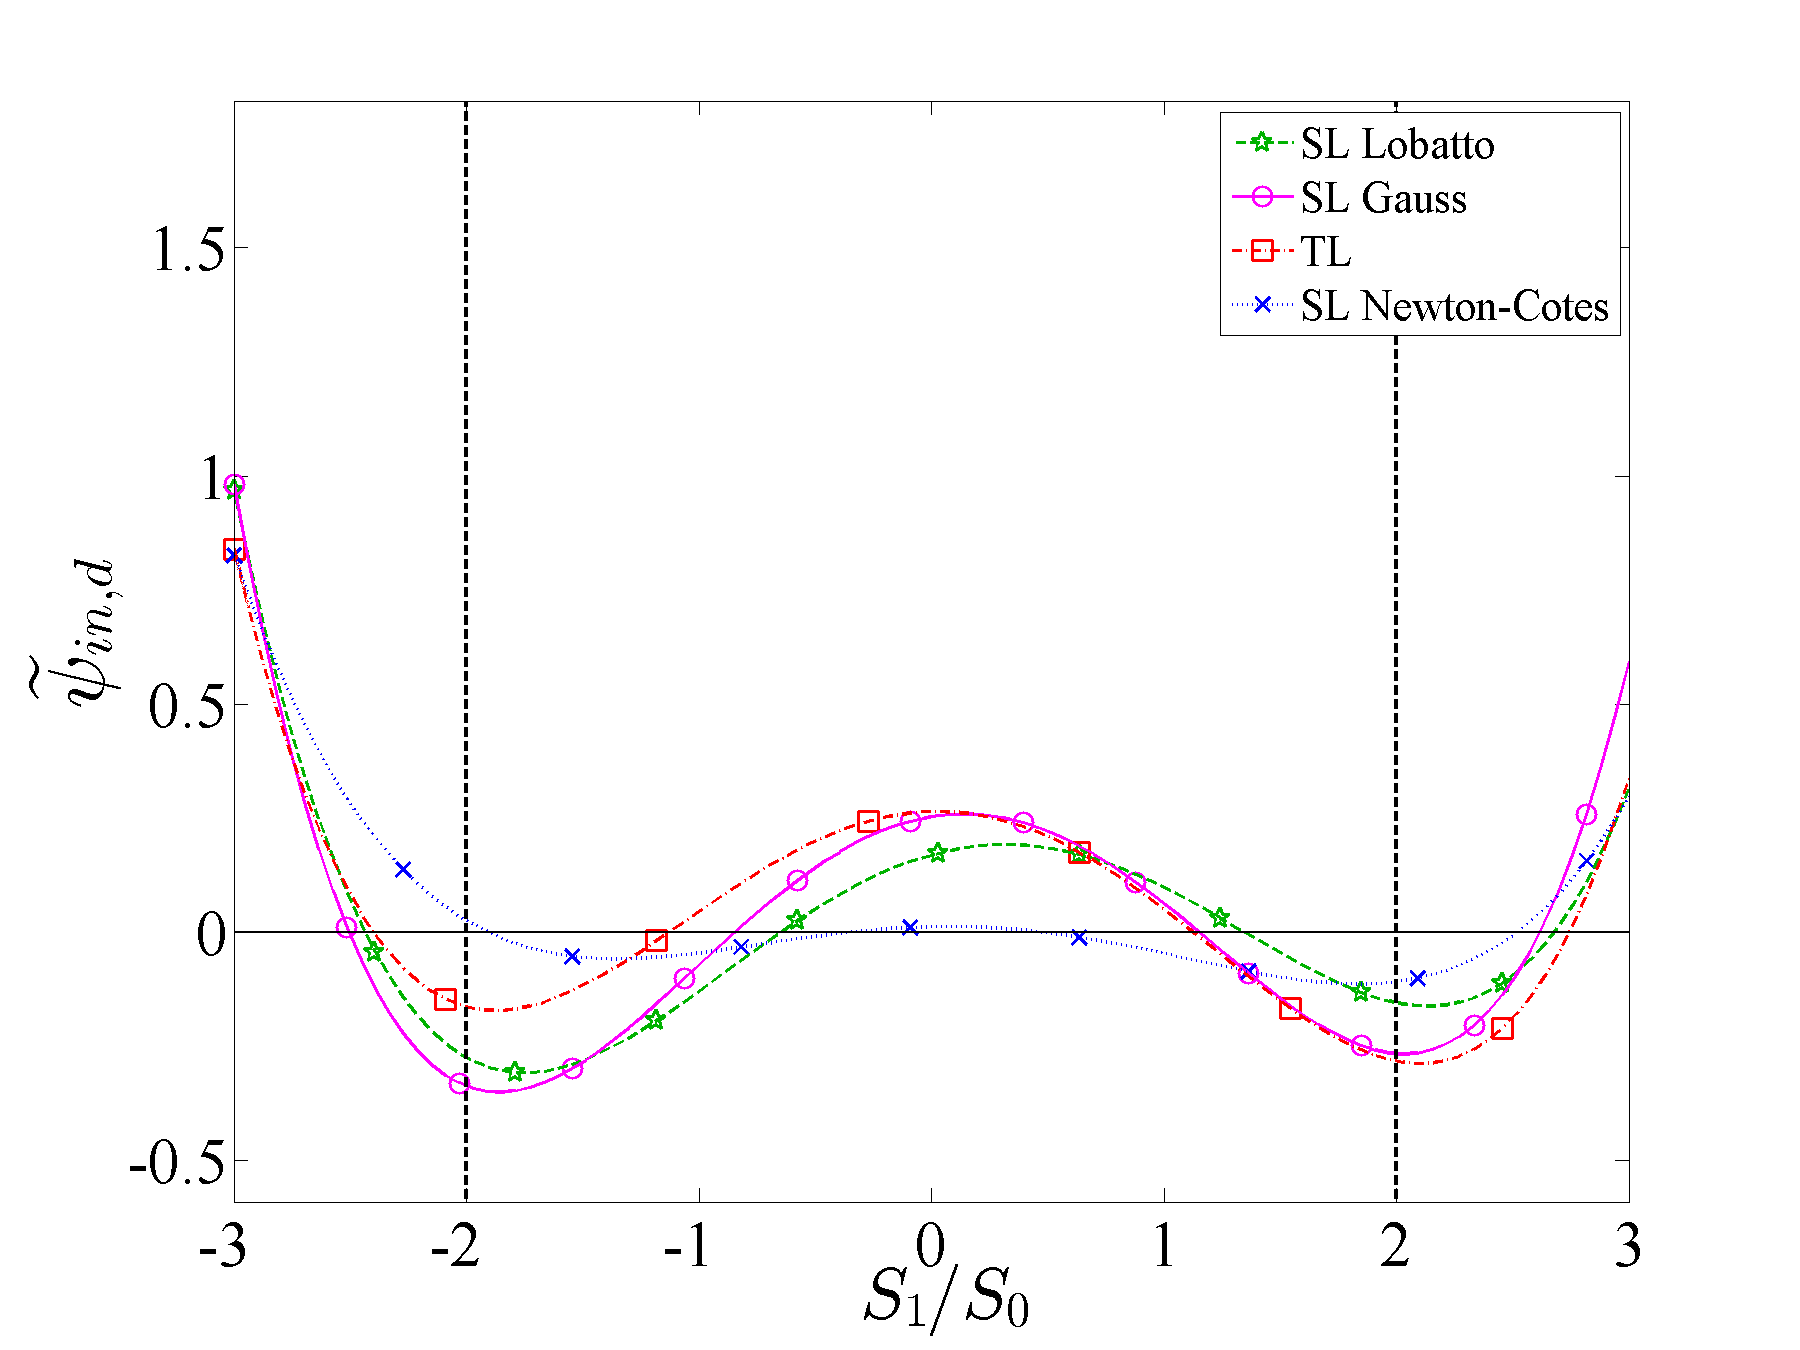
\includegraphics[width=11cm]{chapter2_constant_xs/Final_Inflow_RHS_Comparison_Source_P4_MFP_5.png}
\caption{Numerical inflow values  as a function of $\frac{S_1}{S_0}$, for a single cell (absorber case) with a $\delta$-shaped source, using quartic DFEM.}
\label{fig:abs_inflow_p4}
\end{figure}
\newpage
In \figs{fig:abs_inflow_p1}{fig:abs_inflow_p4}, we again examine the positivity of $\widetilde{\psi}_{in,d}$, but for a non-vacuum case.
Total cell optical thickness was chosen to be 5 mean free paths in \figs{fig:abs_inflow_p1}{fig:abs_inflow_p4} because this value led to the clearest plots.
The relative behaviors observed do not change with cell optical thickness, but using a thicker domain reduces the magnitude for the values of $\widetilde{\psi}_{in,d}$.
All methods in \figs{fig:abs_inflow_p1}{fig:abs_inflow_p4} exactly integrate \eqt{eq:mod_source_moment}.
%, and the scheme naming notation is consistent with \tbl{tbl:names}.
Regardless of trial space chosen,  all schemes exhibit some negativities, but the SL Gauss scheme exhibits the greatest negativities and oscillations. 
The SL Newton-Cotes scheme presents the least severe negativities.


%%%%%%%%%%%%%%%%%%%%%%%%%%%%%%%%%%%%%%%%%%%%%%%%%%%%%%%%%%%%%%%%%%
\subsection{Single-Cell Taylor Series Analysis}
%%%%%%%%%%%%%%%%%%%%%%%%%%%%%%%%%%%%%%%%%%%%%%%%%%%%%%%%%%%%%%%%%%

Next, we perform a local truncation error analysis by comparing the Taylor series expansions for the exact and 
numerical angular fluxes as a function of powers of $h$ for the source-free, incident flux pure absorber problem.  
Matlab \cite{matlab} has been employed to perform the symbolic Taylor series expansions about $h=0$. 
We denote the Taylor-expanded quantities using the subscript $T$. 
The expansions for the analytical inflow, cell average, and outflow are given below:
\begin{subequations}
\label{eq:taylor_ex}
\beanum
\psi_{in,d,T}  &=& \psi_{in,d} \\
\psi_{A,d,T}   &=& \psi_{in,d}\left(1 - \frac{h}{2} + \frac{h^2}{6} - \frac{h^3}{24} + \frac{h^4}{120} - \frac{h^5}{720} \dots     \right)    \\
\psi_{out,d,T} &=& \psi_{in,d}\left(1 - h + \frac{h^2}{2} -\frac{h^3}{6} + \frac{h^4}{24} - \frac{h^5}{120} \dots \right) \pep
\eeanum
\end{subequations}

The Taylor expansions of the numerical analogues to the quantities in \eqts{eq:taylor_ex} depend on the trial space polynomial degree, the choice of interpolatory points, and the numerical integration strategy. 
For brevity, we omit giving these numerical analogues.
Table \ref{tbl:taylor_in_part1} gives the lowest order term for the difference between  $\psi_{in,d,T}$ and the numerical analogs
for the Exact DFEM and TL schemes.  
The same information for the SL Newton-Cotes, SL Gauss, and SL Lobatto schemes is given in \tbl{tbl:taylor_in_part2}.
The differences between $\psi_{A,d,T}$ and the respective numerical analogs are given in \tbl{tbl:taylor_avg_part1} for Exact DFEM and TL,
and \tbl{tbl:taylor_avg_part2} for the SL Newton-Cotes, SL Gauss, and SL Lobatto schemes.
Differences between $\psi{out,d,T}$ and the correseponding numerical analogs are given in \tbl{tbl:taylor_out_part1} for Exact DFEM and TL  and 
\tbl{tbl:taylor_out_part2} gives the lowest order difference between the SL Newton-Cotes, SL Gauss, and SL Lobatto approximations of $\psi_{out,d,T}$.
In Tables \ref{tbl:taylor_in_part1}-\ref{tbl:taylor_out_part2} all entries are listed as
$q(C)$, to be read as ``the difference between the analytic taylor expansion and the numeric analog is $C h^q$ with $h=\Sigma_t \Delta x / \mu$''.
Entries of ``Machine Precision'' in Tables \ref{tbl:taylor_in_part1}-\ref{tbl:taylor_out_part2} are meant to indicate that the difference between
the analytic Taylor expansion and Taylor expansion of the numerical approximation was inconclusive due to all coefficients being within machine precision.
% \begin{landscape}
% \begin{table}[!hbp]
% \centering
% \caption{Local truncation error analysis in $\widetilde{\psi}_{in,d}$ for a single cell problem with constant cross section. 
% Values given as $q(C)$ are to be read as $C h^q$ with $h=\Sigma_t \Delta x / \mu$.}
% \begin{tabular}{|c|c|c|c|c|c|} 
% \hline
  % Polynomial 										  & Exact 										&	 TL  										& SL Newton-Cotes 				& SL Gauss 			 						& SL Lobatto  \\
  % Degree  of $\widetilde{\psi}$		&   DFEM										& {}											& {}		 							 		& {}   										&	 {}   \\
	% \hline
				% 1   											&  2 $(2\times 10^{-1})$		& 2 $(5\times 10^{-1})$		&	2 $(5\times 10^{-1})$		&	2 $(2\times 10^{-1})$		&	2 $(5\times 10^{-1})$	\\
		% \hline
				% 2   											&  3  $(2\times 10^{-2})$		&	3 $(4\times 10^{-2})$		& 3 $(4\times 10^{-2})$		&	3  $(2\times 10^{-2})$	&	3 $(4\times 10^{-2})$		\\
		% \hline	
				% 3   											&  4 $(1\times 10^{-3})$		& 2 $(7\times 10^{-2})$		&	2 $(1\times 10^{-1})$		& 4 $(1\times 10^{-3})$		&	4 $(3\times 10^{-3})$	\\
		% \hline
				% 4   											&  5 $(7\times 10^{-5})$		& 3 $(1\times 10^{-2})$		&	3 $(1\times 10^{-2})$		&	5 $(7\times 10^{-5})$		&	5 $(1\times 10^{-4})$	\\
		% \hline	
				% 5   											&  6 $(3\times 10^{-6})$		& 2 $(5\times 10^{-2})$		&	2 $(6\times 10^{-2})$		&	6 $(3\times 10^{-6})$		&	6 $(7\times 10^{-6})$	\\
		% \hline		
				% 6   											&  7 $(1\times 10^{-7})$		& 3 $(1\times 10^{-2})$		&	3 $(9\times 10^{-3})$		&	7 $(1\times 10^{-7})$		&	7 $(3\times 10^{-7})$	\\
		% \hline		
				% 7   											&  8 $(4\times 10^{-9})$		& 2 $(5\times 10^{-2})$		&	2 $(4\times 10^{-2})$		&	8 $(4\times 10^{-9})$		&	8 $(8\times 10^{-9})$	\\
		% \hline		
% \end{tabular}
% \label{tbl:taylor_in} 
% \end{table}
% \end{landscape}
\begin{table}[!hbp]
\centering
\caption{Local truncation error analysis in $\widetilde{\psi}_{in,d}$ for a single cell problem with constant cross section, for Exact DFEM and TL. }
\begin{tabular}{|c|c|c|} 
\hline
  Polynomial 										  & Exact 										&	 TL                   \\
  Degree  of $\widetilde{\psi}$		&   DFEM										& {}	                  \\
	\hline
				1   											&  2 $(2\times 10^{-1})$		& 2 $(5\times 10^{-1})$		\\
		\hline
				2   											&  3  $(2\times 10^{-2})$		&	3 $(4\times 10^{-2})$	\\
		\hline	
				3   											&  4 $(1\times 10^{-3})$		& 2 $(7\times 10^{-2})$	\\
		\hline
				4   											&  5 $(7\times 10^{-5})$		& 3 $(1\times 10^{-2})$	\\
		\hline	
				5   											&  6 $(3\times 10^{-6})$		& 2 $(5\times 10^{-2})$	\\
		\hline		
				6   											&  7 $(1\times 10^{-7})$		& 3 $(1\times 10^{-2})$	\\
		\hline		
				7   											&  8 $(4\times 10^{-9})$		& 2 $(5\times 10^{-2})$	\\
		\hline		
\end{tabular}
\label{tbl:taylor_in_part1} 
\end{table}
\begin{table}[!htp]
\centering
\caption{Local truncation error analysis in $\widetilde{\psi}_{in,d}$ for a single cell problem with constant cross section, for SL Newton-Cotes, SL Gauss, and SL Lobatto. }
\begin{tabular}{|c|c|c|c|} 
\hline
  Polynomial 										 & SL Newton-Cotes 				& SL Gauss 			 						& SL Lobatto  \\
  Degree  of $\widetilde{\psi}$	& {}		 							 		& {}   										&	 {}   \\
	\hline
				1   										&	2 $(5\times 10^{-1})$		&	2 $(2\times 10^{-1})$		&	2 $(5\times 10^{-1})$	\\
		\hline
				2   										& 3 $(4\times 10^{-2})$		&	3  $(2\times 10^{-2})$	&	3 $(4\times 10^{-2})$		\\
		\hline	
				3   										&	2 $(1\times 10^{-1})$		& 4 $(1\times 10^{-3})$		&	4 $(3\times 10^{-3})$	\\
		\hline
				4   										&	3 $(1\times 10^{-2})$		&	5 $(7\times 10^{-5})$		&	5 $(1\times 10^{-4})$	\\
		\hline	
				5   										&	2 $(6\times 10^{-2})$		&	6 $(3\times 10^{-6})$		&	6 $(7\times 10^{-6})$	\\
		\hline		
				6   										&	3 $(9\times 10^{-3})$		&	7 $(1\times 10^{-7})$		&	7 $(3\times 10^{-7})$	\\
		\hline		
				7   										&	2 $(4\times 10^{-2})$		&	8 $(4\times 10^{-9})$		&	8 $(8\times 10^{-9})$	\\
		\hline		
\end{tabular}
\label{tbl:taylor_in_part2} 
\end{table}
%
%
% \begin{table}[!htp]
% \centering
% \caption{Local truncation error analysis in $\widetilde{\psi}_{A,d}$ for a single cell problem with constant cross section, for Exact DFEM and TL.}
% \begin{tabular}{|c|c|c|c|c|c|} 
% \hline
  % Polynomial 										  & Exact 											& TL  										& SL Newton-Cotes 					& SL Gauss 			 						& SL Lobatto  \\
  % Degree  of $\widetilde{\psi}$		&   DFEM											& {}											& {}		 							 			& {}   											&	 {}   \\
  	% \hline
				% 1   											&  	3 $(1\times 10^{-2})$			& 2 $(2\times 10^{-1})$		&	2 $(2\times 10^{-1})$			&	3 $(1\times 10^{-2})$			&	2 $(2\times 10^{-1})$		\\
		% \hline
				% 2   											&   5 $(1\times 10^{-4})$			&  4 $(2\times 10^{-3})$	&	4 $(2\times 10^{-3})$			&	5 $(1\times 10^{-4})$			&	4 $(2\times 10^{-3})$		\\
		% \hline	
				% 3   											&   7 $(7\times 10^{-7})$			& 3 $(3\times 10^{-3})$		&	4 $(6\times 10^{-4})$			&	 7 $(7\times 10^{-7})$		&	6 $(1\times 10^{-5})$\\
		% \hline
				% 4   											&  9 $(2\times 10^{-9})$			& 5 $(8\times 10^{-5})$		&	6 $(8\times 10^{-6})$			&	9 $(2\times 10^{-9})$			&	8 $(5\times 10^{-8})$	\\
		% \hline
				% 5   											&  11 $(5\times 10^{-12})$		& 3 $(1\times 10^{-3})$		&	6 $(2\times 10^{-6})$			&	11 $(5\times 10^{-12})$		&	10 $(1\times 10^{-10})$\\
		% \hline	
				% 6   											&  13 $(7\times 10^{-15})$		& 5 $(7\times 10^{-5})$		&	8 $(2\times 10^{-8})$			&	13 $(7\times 10^{-15})$		&	12 $(2\times 10^{-13})$\\
		% \hline
				% 7   											&  Machine Precision					& 3 $(1\times 10^{-3})$		&	8 $(3\times 10^{-9})$			&	Machine Precision					&	Machine Precision   \\
		% \hline	
% \end{tabular}
% \label{tbl:taylor_avg} 
% \end{table}
% \end{landscape}
% \pagebreak
% \begin{landscape}
% \begin{table}[!hbp]
% \centering
% \caption{Local truncation error analysis in $\widetilde{\psi}_{out,d}$ for a single cell with constant cross section, for SL Newton-Cotes, SL Gauss, and SL Lobatto.}
% \begin{tabular}{|c|c|c|c|c|c|} 
% \hline
  % Polynomial 										  & Exact 										& TL  										& SL Newton-Cotes 					& SL Gauss 			 					& SL Lobatto  \\
  % Degree  of $\widetilde{\psi}$		&   DFEM										& {}											& {}		 							 			& {}   										&	 {}   \\
  	% \hline
				% 1   											&  4 $(1\times 10^{-2})$		& 3 $(2\times 10^{-1})$		&	3 $(2\times 10^{-1})$		&	4 $(1\times 10^{-2})$			&	3 $(2\times 10^{-1})$	\\
		% \hline
				% 2   											&  6 $(1\times 10^{-4})$		& 5 $(2\times 10^{-3})$		&	5 $(2\times 10^{-3})$			&	6 $(1\times 10^{-4})$		&	5 $(2\times 10^{-3})$		\\
		% \hline	
				% 3   											&  8 $(7\times 10^{-7})$		& 4 $(3\times 10^{-3})$		&	5 $(6\times 10^{-4})$		&	8 $(7\times 10^{-7})$			&	7 $(1\times 10^{-5})$	\\
		% \hline
				% 4   											&  10 $(2\times 10^{-9})$		& 6 $(1\times 10^{-2})$		&	7 $(8\times 10^{-6})$		&	10 $(2\times 10^{-9})$		&	9 $(5\times 10^{-8})$	\\
		% \hline
				% 5   											&  12 $(5\times 10^{-12})$	& 4 $(1\times 10^{-3})$		&	7 $(2\times 10^{-6})$		&	12 $(5\times 10^{-12})$		&	11 $(1\times 10^{-10})$	\\
		% \hline		
				% 6   											&  14 $(7\times 10^{-15})$	& 6 $(7\times 10^{-5})$		&	9 $(2\times 10^{-8})$		&	14 $(7\times 10^{-15})$		&	13 $(2\times 10^{-13})$\\
		% \hline
				% 7   											&  Machine Precision				& 4 $(1\times 10^{-3})$		&	9 $(3\times 10^{-9})$		& Machine Precision					&	Machine Precision  \\
		% \hline
% \end{tabular}
% \label{tbl:taylor_out} 
% \end{table}
% \end{landscape}
\begin{table}[!htp]
\centering
\caption{Local truncation error analysis in $\widetilde{\psi}_{A,d}$ for a single cell problem with constant cross section, for Exact DFEM and TL.}
\begin{tabular}{|c|c|c||} 
\hline
  Polynomial 										  & Exact 											& TL   \\
  Degree  of $\widetilde{\psi}$		&   DFEM											& {}	 \\
  	\hline
				1   											&  	3 $(1\times 10^{-2})$			& 2 $(2\times 10^{-1})$		 \\
		\hline
				2   											&   5 $(1\times 10^{-4})$			&  4 $(2\times 10^{-3})$	\\
		\hline	
				3   											&   7 $(7\times 10^{-7})$			& 3 $(3\times 10^{-3})$	\\
		\hline
				4   											&  9 $(2\times 10^{-9})$			& 5 $(8\times 10^{-5})$	\\
		\hline
				5   											&  11 $(5\times 10^{-12})$		& 3 $(1\times 10^{-3})$	\\
		\hline	
				6   											&  13 $(7\times 10^{-15})$		& 5 $(7\times 10^{-5})$	\\
		\hline
				7   											&  Machine Precision					& 3 $(1\times 10^{-3})$  \\
		\hline	
\end{tabular}
\label{tbl:taylor_avg_part1} 
\end{table}
\begin{table}[!hbp]
\centering
\caption{Local truncation error analysis in $\widetilde{\psi}_{A,d}$ for a single cell problem with constant cross section, for SL Newton-Cotes, SL Gauss, and SL Lobatto}
\begin{tabular}{|c|c|c|c|} 
\hline
  Polynomial 										 & SL Newton-Cotes 					& SL Gauss 			 						& SL Lobatto  \\
  Degree  of $\widetilde{\psi}$	  & {}		 							 			& {}   											&	 {}   \\
  	\hline
				1   									  &	2 $(2\times 10^{-1})$			&	3 $(1\times 10^{-2})$			&	2 $(2\times 10^{-1})$		\\
		\hline
				2   							     &	4 $(2\times 10^{-3})$			&	5 $(1\times 10^{-4})$			&	4 $(2\times 10^{-3})$		\\
		\hline	
				3   								  	&	4 $(6\times 10^{-4})$			&	 7 $(7\times 10^{-7})$		&	6 $(1\times 10^{-5})$\\
		\hline
				4   									  &	6 $(8\times 10^{-6})$			&	9 $(2\times 10^{-9})$			&	8 $(5\times 10^{-8})$	\\
		\hline
				5   								  	&	6 $(2\times 10^{-6})$			&	11 $(5\times 10^{-12})$		&	10 $(1\times 10^{-10})$\\
		\hline	
				6   								  	&	8 $(2\times 10^{-8})$			&	13 $(7\times 10^{-15})$		&	12 $(2\times 10^{-13})$\\
		\hline
				7   								  	&	8 $(3\times 10^{-9})$			&	Machine Precision					&	Machine Precision   \\
		\hline	
\end{tabular}
\label{tbl:taylor_avg_part2} 
\end{table}
%
\pagebreak
%
\begin{table}[!htp]
\centering
\caption{Local truncation error analysis in $\widetilde{\psi}_{out,d}$ for a single cell with constant cross section, for Exact DFEM and TL.}
\begin{tabular}{|c|c|c|} 
\hline
  Polynomial 										  & Exact 										& TL  	\\
  Degree  of $\widetilde{\psi}$		&   DFEM										& {}	\\
  	\hline
				1   											&  4 $(1\times 10^{-2})$		& 3 $(2\times 10^{-1})$	\\
		\hline
				2   											&  6 $(1\times 10^{-4})$		& 5 $(2\times 10^{-3})$	\\
		\hline	
				3   											&  8 $(7\times 10^{-7})$		& 4 $(3\times 10^{-3})$	\\
		\hline
				4   											&  10 $(2\times 10^{-9})$		& 6 $(1\times 10^{-2})$	\\
		\hline
				5   											&  12 $(5\times 10^{-12})$	& 4 $(1\times 10^{-3})$	\\
		\hline		
				6   											&  14 $(7\times 10^{-15})$	& 6 $(7\times 10^{-5})$	\\
		\hline
				7   											&  Machine Precision				& 4 $(1\times 10^{-3})$	\\
		\hline
\end{tabular}
\label{tbl:taylor_out_part1} 
\end{table}
%
%
\begin{table}[!htp]
\centering
\caption{Local truncation error analysis in $\widetilde{\psi}_{out,d}$ for a single cell with constant cross section, for SL Newton-Cotes, SL Gauss, and SL Lobatto.}
\begin{tabular}{|c|c|c|c|} 
\hline
  Polynomial 										 & SL Newton-Cotes 					& SL Gauss 			 					& SL Lobatto  \\
  Degree  of $\widetilde{\psi}$	& {}		 							 			& {}   										&	 {}   \\
  	\hline
				1   										&	3 $(2\times 10^{-1})$		&	4 $(1\times 10^{-2})$			&	3 $(2\times 10^{-1})$	\\
		\hline
				2   										&	5 $(2\times 10^{-3})$			&	6 $(1\times 10^{-4})$		&	5 $(2\times 10^{-3})$		\\
		\hline	
				3   										&	5 $(6\times 10^{-4})$		&	8 $(7\times 10^{-7})$			&	7 $(1\times 10^{-5})$	\\
		\hline
				4   										&	7 $(8\times 10^{-6})$		&	10 $(2\times 10^{-9})$		&	9 $(5\times 10^{-8})$	\\
		\hline
				5   										&	7 $(2\times 10^{-6})$		&	12 $(5\times 10^{-12})$		&	11 $(1\times 10^{-10})$	\\
		\hline		
				6   										&	9 $(2\times 10^{-8})$		&	14 $(7\times 10^{-15})$		&	13 $(2\times 10^{-13})$\\
		\hline
				7   										&	9 $(3\times 10^{-9})$		& Machine Precision					&	Machine Precision  \\
		\hline
\end{tabular}
\label{tbl:taylor_out_part2} 
\end{table}

This local truncation error analysis illustrates the following. 
\begin{enumerate}
\item Exact DFEM and SL Gauss, which are equivalent, exactly integrate the mass matrix, and are the most accurate,
\item TL does not guarantee increasing order of accuracy by using higher degree polynomial trial spaces,
\item TL converges at most third or fifth order for $\widetilde{\psi}_{A,d}$ and fourth or sixth order for $\widetilde{\psi}_{out,d}$ for odd or even polynomial trial spaces, respectively,
\item SL Newton-Cotes increases in accuracy with higher degree polynomial trial spaces, but only for $\widetilde{\psi}_{out,d}$ and $\widetilde{\psi}_{A,d}$,
\item TL and SL Newton-Cotes are at most second order or third order accurate for $\widetilde{\psi}_{in,d}$ for odd or even polynomial trial spaces, respectively, 
\item SL Gauss is order $2P+1$ accurate in calculating $\widetilde{\psi}_{A,d}$ and order $2P+2$ accurate in calculating $\widetilde{\psi}_{out,d}$,
\item SL Lobatto is order $2P$ accurate in calculating $\widetilde{\psi}_{A,d}$ and order $2P+1$ in calculating $\widetilde{\psi}_{out,d}$, 
%\item SL Gauss is up to an order of $h$ more accurate than SL Lobatto for a given $P$ in calculating $\widetilde{\psi}_A$ and $\widetilde{\psi}_{out}$, 
\item SL Gauss, SL Lobatto, and Exact DFEM are accurate to order $P+1$ in calculating $\widetilde{\psi}_{in,d}$, and
\item SL Gauss is more accurate than SL Lobatto (smaller error constant) in computing $\widetilde{\psi}_{in,d}$, but not an order of $h$ .
\end{enumerate}

%%%%%%%%%%%%%%%%%%%%%%%%%%%%%%%%%%%%%%%%%%%%%%%%%%%%%%%%%%%%%%%%%%
\subsection{Convergence Rates for Spatially Discretized 1-D Domains}
\label{sec:multi_cell}
%%%%%%%%%%%%%%%%%%%%%%%%%%%%%%%%%%%%%%%%%%%%%%%%%%%%%%%%%%%%%%%%%%

Here, we consider a homogeneous pure absorber material placed in a 1-D slab configuration and uniformly mesh the domain using $N_{cells}$ cells. 
We use: $x\in[0,10~cm]$, $\Sigma_{t}=1~[cm^{-1}]$, no external sources, vacuum conditions on the right face of the slab, and a normally incident unit beam on the left face.
%\benum
%\psi_{in,d} = \left \{ \begin{array}{ll}
%1 ~&~\mu_d=1 \\
%0 ~&~\text{otherwise}
%\end{array}
%\right. \pep
%\eenum
The analytical solution to this problem is trivial to obtain:
\benum
\psi(x,\mu_d) = \left \{ \begin{array}{ll}  \exp\left[-\Sigma_t x \right] & \mu_d =1 \\ 0 & \text{otherwise} \end{array} \right. \pep
\eenum
The $L_2$ norm of the error is:
\benum
%E_{\psi} = \sqrt{ \int_{0}^{10~[cm]}{ \left(\psi(x,\mu_d) - \widetilde{\psi}_{d,i}(x)  \right)^2~dx}}
E_{\psi} 
= \sqrt{\sum_{i=1}^{N_{cells}}{ \int_{x_{i-1/2}}^{x_{i+1/2}}{ \left(\psi(x,\mu_d) - \widetilde{\psi}_{d,i}(x)  \right)^2~dx}}} \pec
\eenum
where we recall that $\widetilde{\psi}_{d,i}(x)$ is the DFEM approximation of the angular flux in cell $i$.
To evaluate the above integral, we use a high-order Gauss quadrature set  ($x_{\textit{f,q}}, \, w_{\textit{f,q}}$) that employs a large number of quadrature points:
\benum
E_{\psi} \approx \sqrt{\sum_{i=1}^{N_{cells}}{ \frac{\Delta x_i}{2} \sum_{q=1}^{N_{\textit{qf}}}{w_{\textit{f,q}}\left(\psi(x_{\textit{f,q}},\mu_d) - \widetilde{\psi}_d(x_{\textit{f,q}})  \right)^2}}} \pep
\label{eq:l2}
\eenum
Values of $E_{\psi}$ shown here are calculated using $N_{\textit{qf}}=10$.  
In addition to the $L_2$ error, we also present the cell average angular flux error, $E_{\psi_A}$, defined as
\benum
E_{\psi_A} = \sqrt{\sum_{i=1}^{N_{cells}}{ \Delta x_i\left(\psi_{A,d,i} - \widetilde{\psi}_{A,d,i} \right)^2}} \pec
\label{eq:l2A}
\eenum
and the cell outflow error, $E_{\psi_{out}}$, given by:
\benum
E_{\psi_{out}} = \sqrt{\sum_{i=1}^{N_{cells}}{ \Delta x_i\left(\psi(x_{i+1/2},\mu_d) - \widetilde{\psi}_{out,d,i}  \right)^2}} \pep  
\label{eq:l2Out} 
\eenum
%
%
%
In \eqt{eq:l2}, \eqt{eq:l2A}, and \eqt{eq:l2Out}, $\Delta x_i$ is the cell width of cell $i$ and $\psi_{A,d,i}$ is the exact cell-averaged angular flux in cell $i$, which, for $\mu_d=1$, is simply:
\beanum
\psi_{A,d,i} =  \exp[-\Sigma_t x_{i-1/2}]\frac{1}{\Delta x_i}\left(1-\exp[-\Sigma_t \Delta x_i] \right) \pep
\eeanum
In the plots that follow, we omit plotting the errors of Exact DFEM since the Exact DFEM solution is identical to that of SL Gauss.  
For linear and quadratic polynomials, we plot only SL Lobatto and omit plotting TL and SL Newton-Cotes since these methods yield identical solutions for linear and quadratic trial spaces.  
\begin{figure}[!htp]
\centering
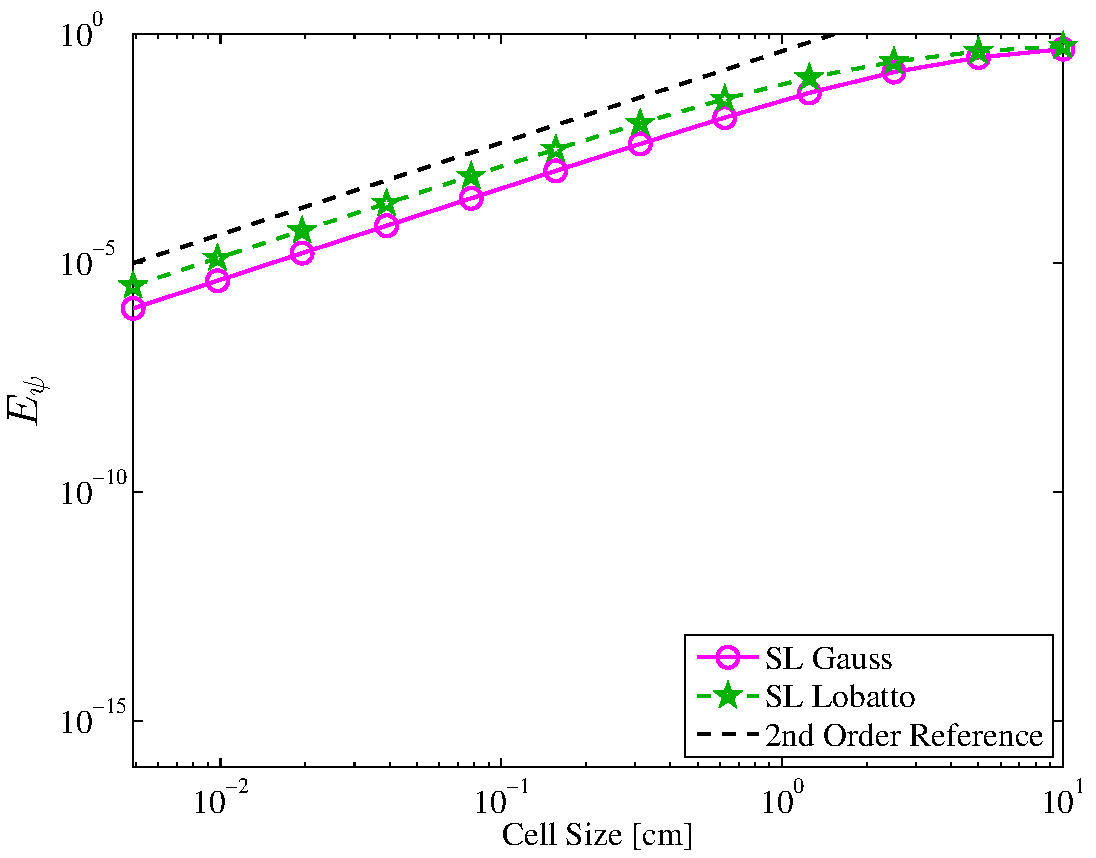
\includegraphics[width=11cm]{chapter2_constant_xs/Linear_L2_err-eps-converted-to.pdf}
\caption{Convergence rate of the $L_2$ norm of the error, $E_{\psi}$,  as a function of the mesh cell size for a pure absorber discretized with linear DFEM.}
\label{fig:multi_L2_p1}
\end{figure}
\begin{figure}[!htp]
\centering
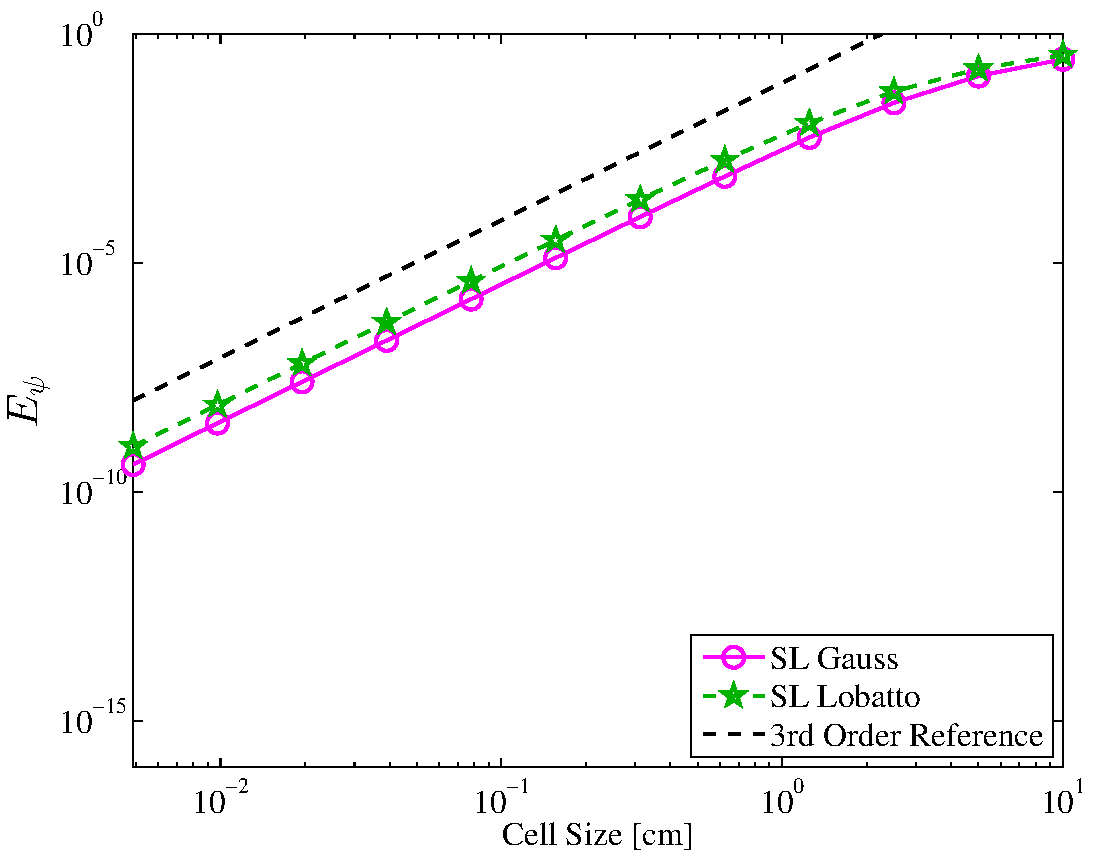
\includegraphics[width=11cm]{chapter2_constant_xs/Quadratic_L2_err-eps-converted-to.pdf}
\caption{Convergence rate of the $L_2$ norm of the error, $E_{\psi}$,  as a function of the mesh cell size for a pure absorber discretized with quadratic DFEM.}
\label{fig:multi_L2_p2}
\end{figure}
\begin{figure}[!hbp]
\centering
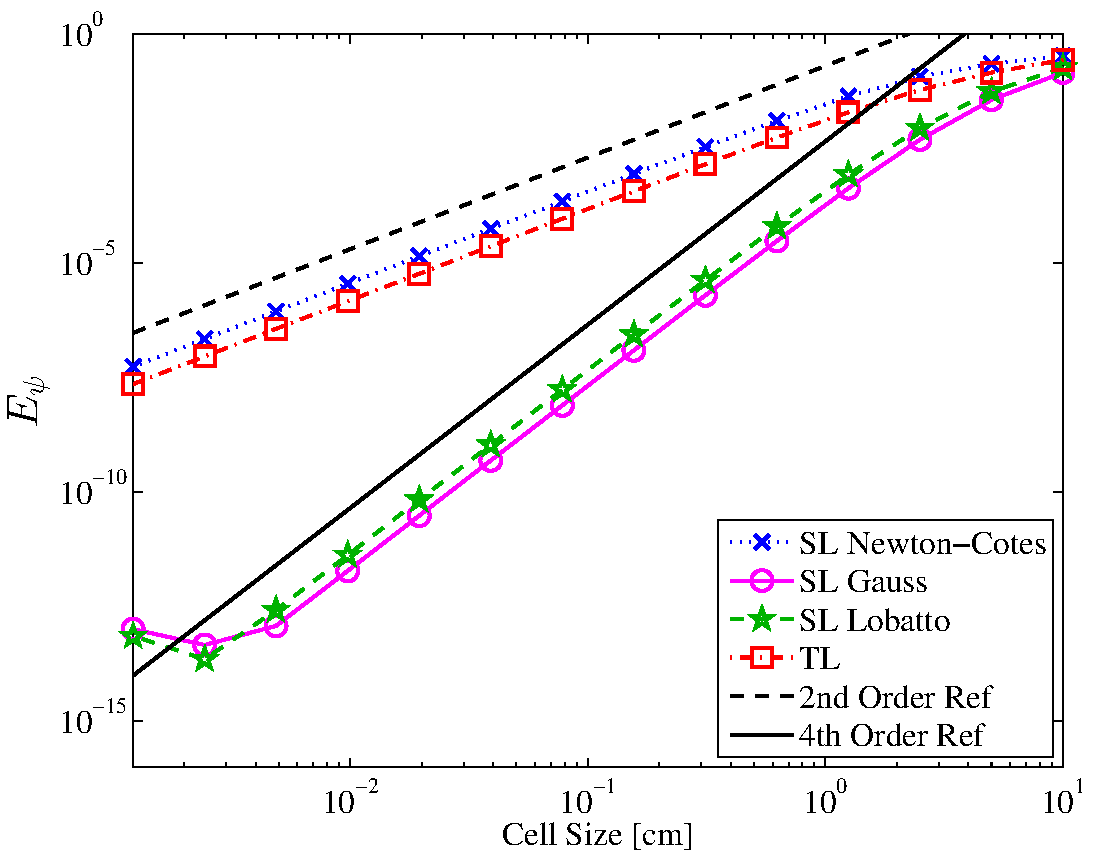
\includegraphics[width=11cm]{chapter2_constant_xs/Cubic_L2_err-eps-converted-to.pdf}
\caption{Convergence rate of the $L_2$ norm of the error, $E_{\psi}$,  as a function of the mesh cell size for a pure absorber discretized with cubic DFEM.}
\label{fig:multi_L2_p3}
\end{figure}
\begin{figure}[!htp]
\centering
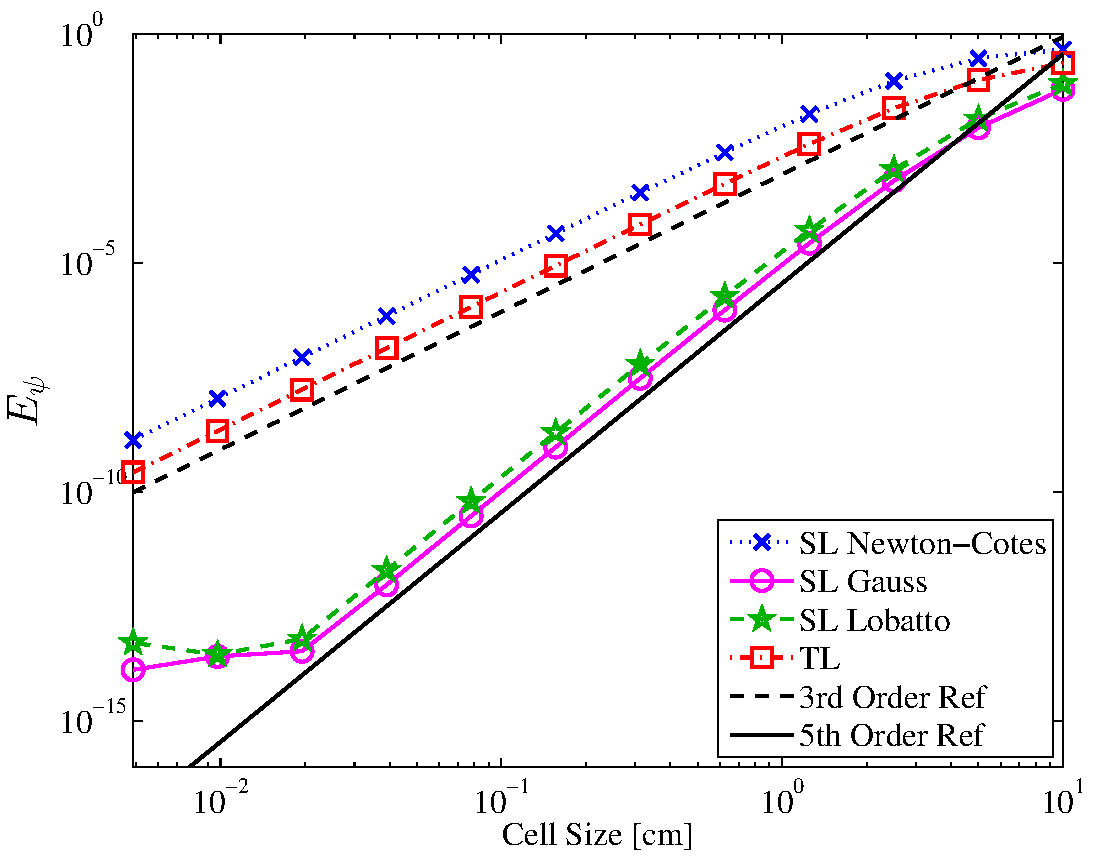
\includegraphics[width=11cm]{chapter2_constant_xs/Quartic_L2_err-eps-converted-to.pdf}
\caption{Convergence rate of the $L_2$ norm of the error, $E_{\psi}$,  as a function of the mesh cell size for a pure absorber discretized with quartic DFEM.}
\label{fig:multi_L2_p4}
\end{figure}
Figures \ref{fig:multi_L2_p1}-\ref{fig:multi_L2_p4} mirror the results of \tbl{tbl:taylor_in_part1} and \tbl{tbl:taylor_in_part2}, which is expected since the convergence rate of $E_{\psi}$ will be limited by the slowest converging local approximation which is $\widetilde{\psi}_{in,d}$.  
Similarly, \figs{fig:multi_L2A_p1}{fig:multi_L2A_p4} are the multiple-cell analogue of the local truncation error analysis of $\widetilde{\psi}_{A,d}$ given in \tbl{tbl:taylor_avg_part1} and \tbl{tbl:taylor_avg_part2}.  
\begin{figure}[!hbp]
\centering
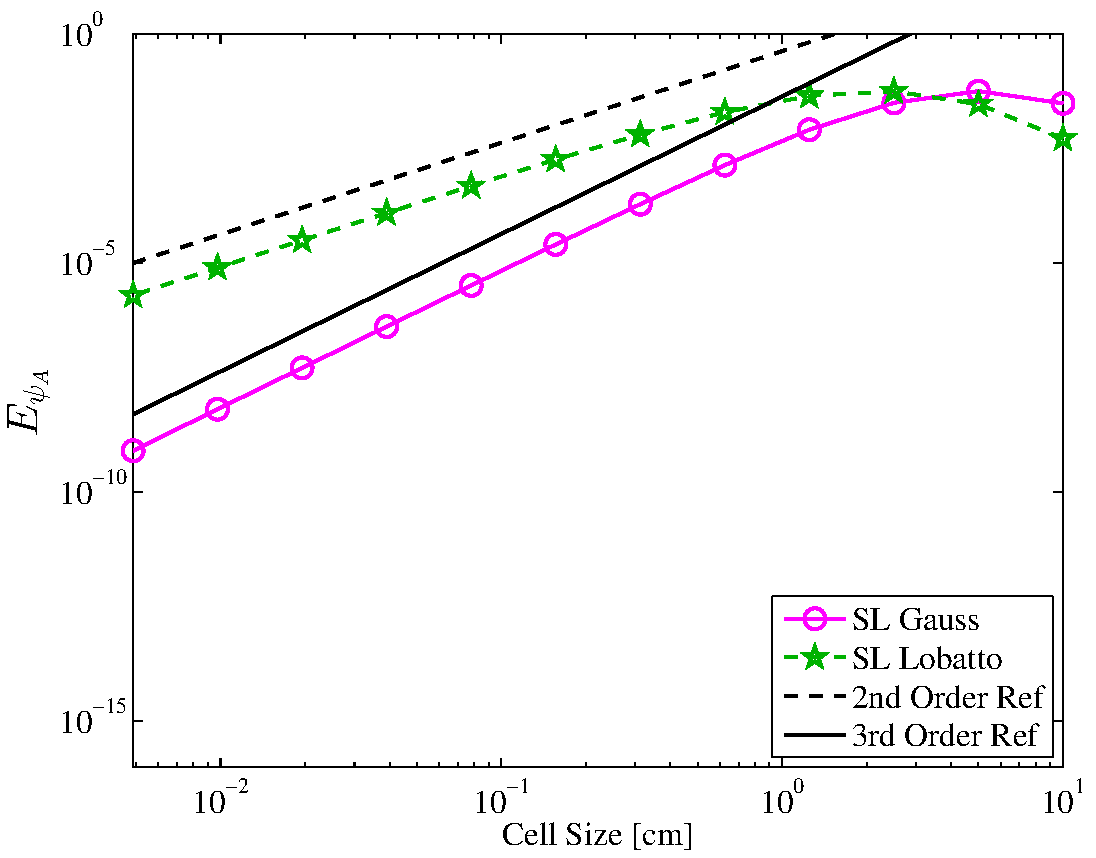
\includegraphics[width=11cm]{chapter2_constant_xs/Linear_L2A_err-eps-converted-to.pdf}
\caption{Convergence rate for $E_{\psi,A}$ as a function of the mesh cell size for a homogeneous pure absorber and linear DFEM.}
\label{fig:multi_L2A_p1}
\end{figure}
\begin{figure}[!htp]
\centering
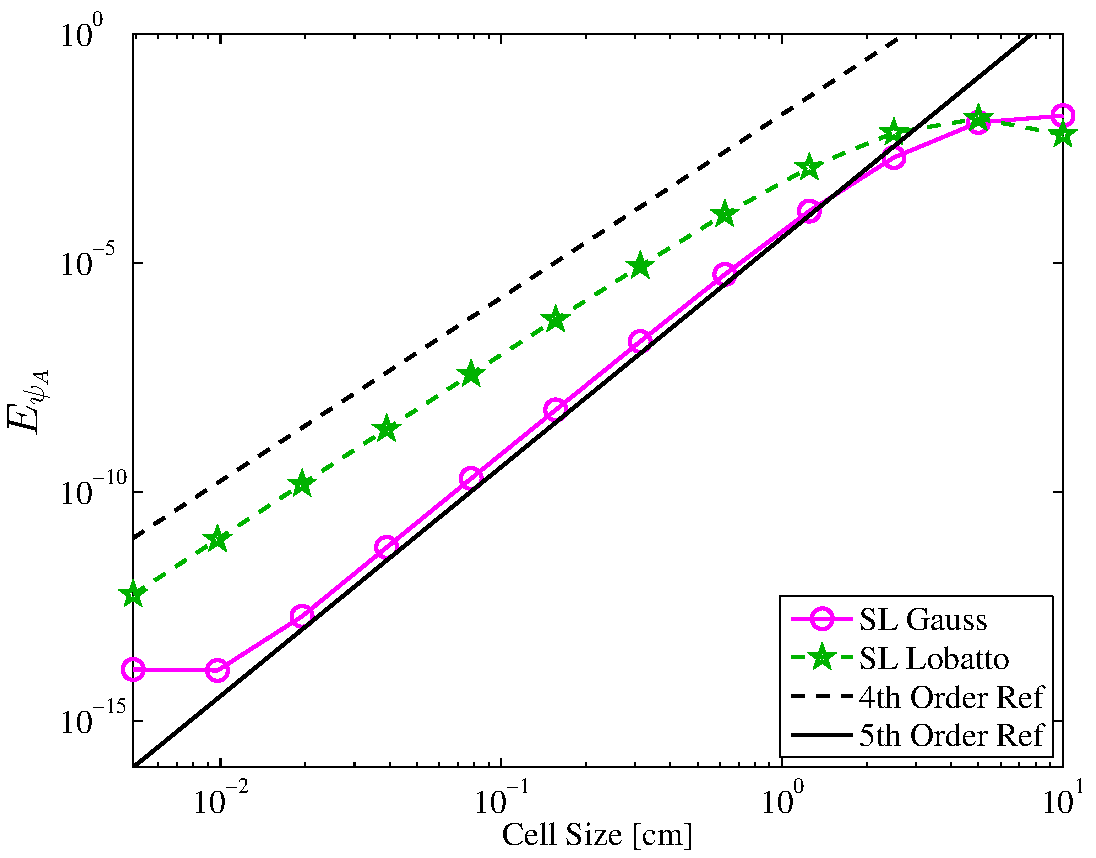
\includegraphics[width=11cm]{chapter2_constant_xs/Quadratic_L2A_err-eps-converted-to.pdf}
\caption{Convergence rate for $E_{\psi,A}$ as a function of the mesh cell size for a homogeneous pure absorber and quadratic DFEM.}
\label{fig:multi_L2A_p2}
\end{figure}
\begin{figure}[!hbp]
\centering
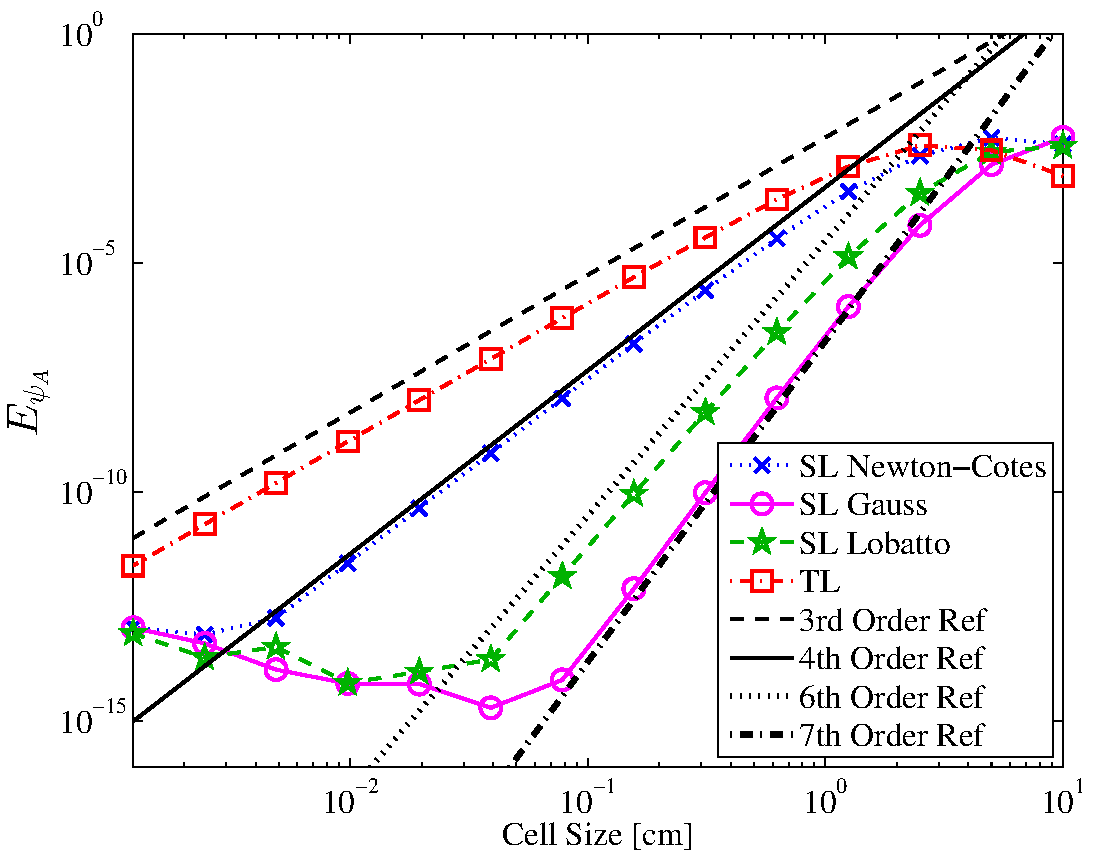
\includegraphics[width=11cm]{chapter2_constant_xs/Cubic_L2A_err-eps-converted-to.pdf}
\caption{Convergence rate for $E_{\psi,A}$ as a function of the mesh cell size for a homogeneous pure absorber and cubic DFEM.}
\label{fig:multi_L2A_p3}
\end{figure}
\begin{figure}[!htp]
\centering
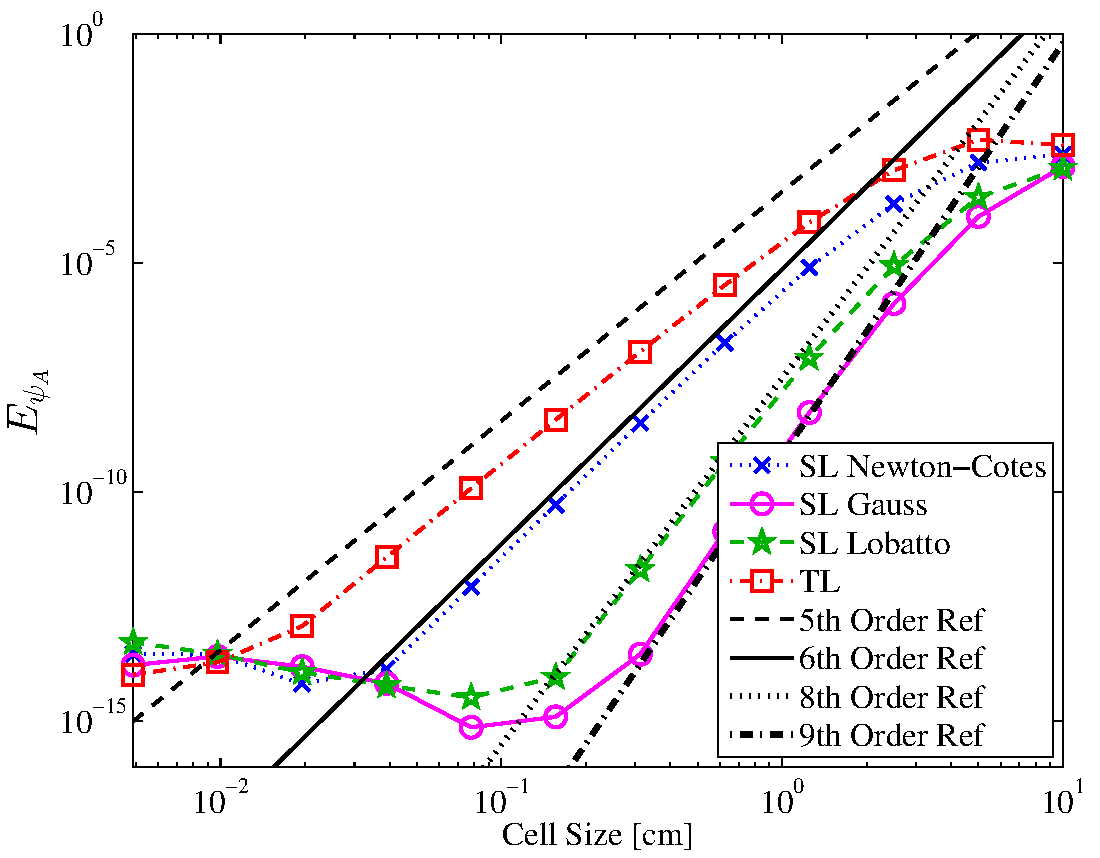
\includegraphics[width=11cm]{chapter2_constant_xs/Quartic_L2A_err-eps-converted-to.pdf}
\caption{Convergence rate for $E_{\psi,A}$ as a function of the mesh cell size for a homogeneous pure absorber and quartic DFEM.}
\label{fig:multi_L2A_p4}
\end{figure}
$E_{\psi_{out}}$, as shown in \figs{fig:multi_L2Out_p1}{fig:multi_L2Out_p4}, does not converge at the local truncation error rates of \tbl{tbl:taylor_out_part1} and \tbl{tbl:taylor_out_part2}.  
%

%
%
\begin{figure}[!hbp]
\centering
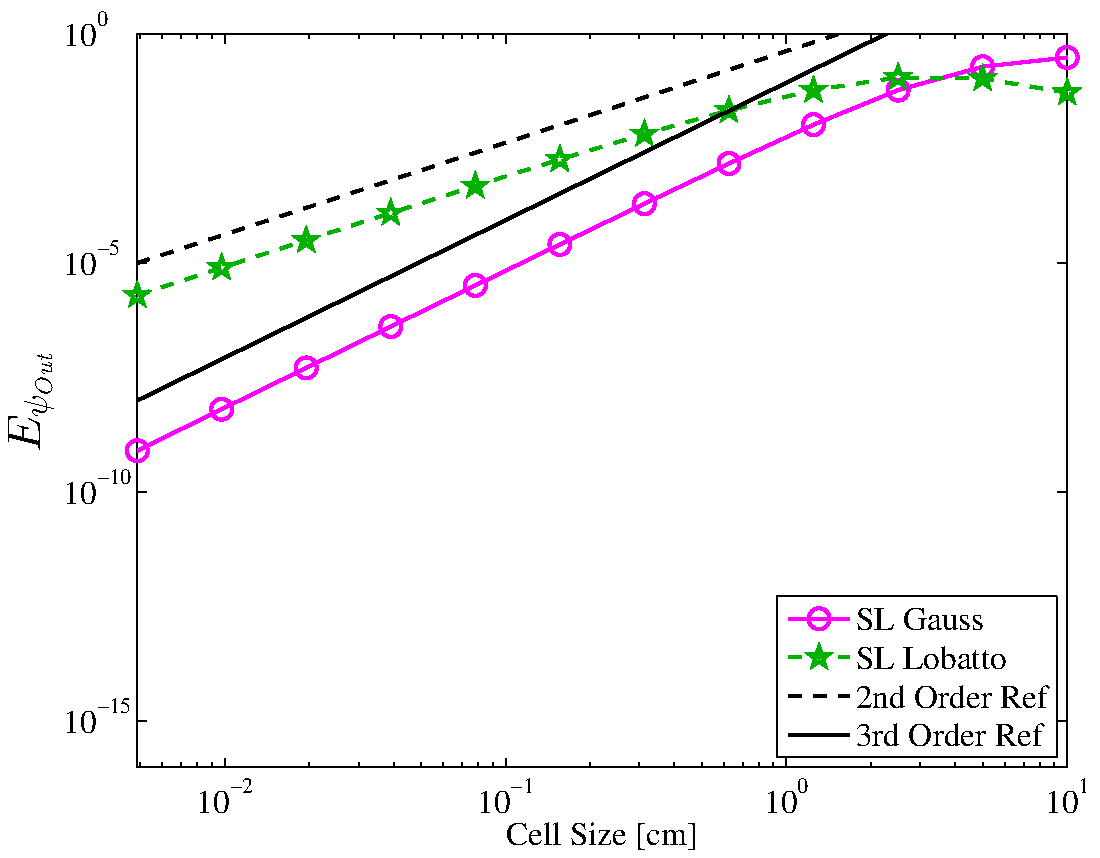
\includegraphics[width=11cm]{chapter2_constant_xs/Linear_L2Out_err-eps-converted-to.pdf}
\caption{Convergence rate of $E_{\psi,out}$ as a function of the mesh cell size for a homogeneous pure absorber for linear DFEM.}
\label{fig:multi_L2Out_p1}
\end{figure}
\begin{figure}[!htp]
\centering
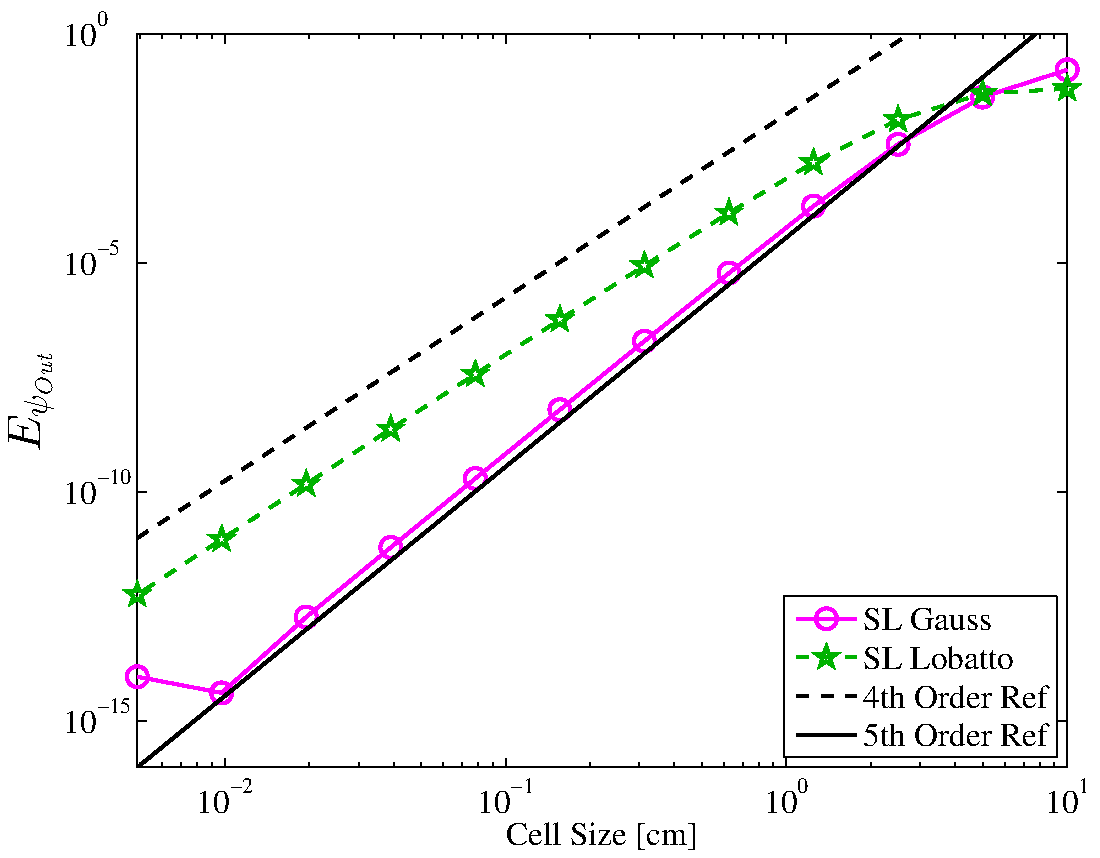
\includegraphics[width=11cm]{chapter2_constant_xs/Quadratic_L2Out_err-eps-converted-to.pdf}
\caption{Convergence rate of $E_{\psi,out}$ as a function of the mesh cell size for a homogeneous pure absorber for quadratic DFEM.}
\label{fig:multi_L2Out_p2}
\end{figure}
\begin{figure}[!hbp]
\centering
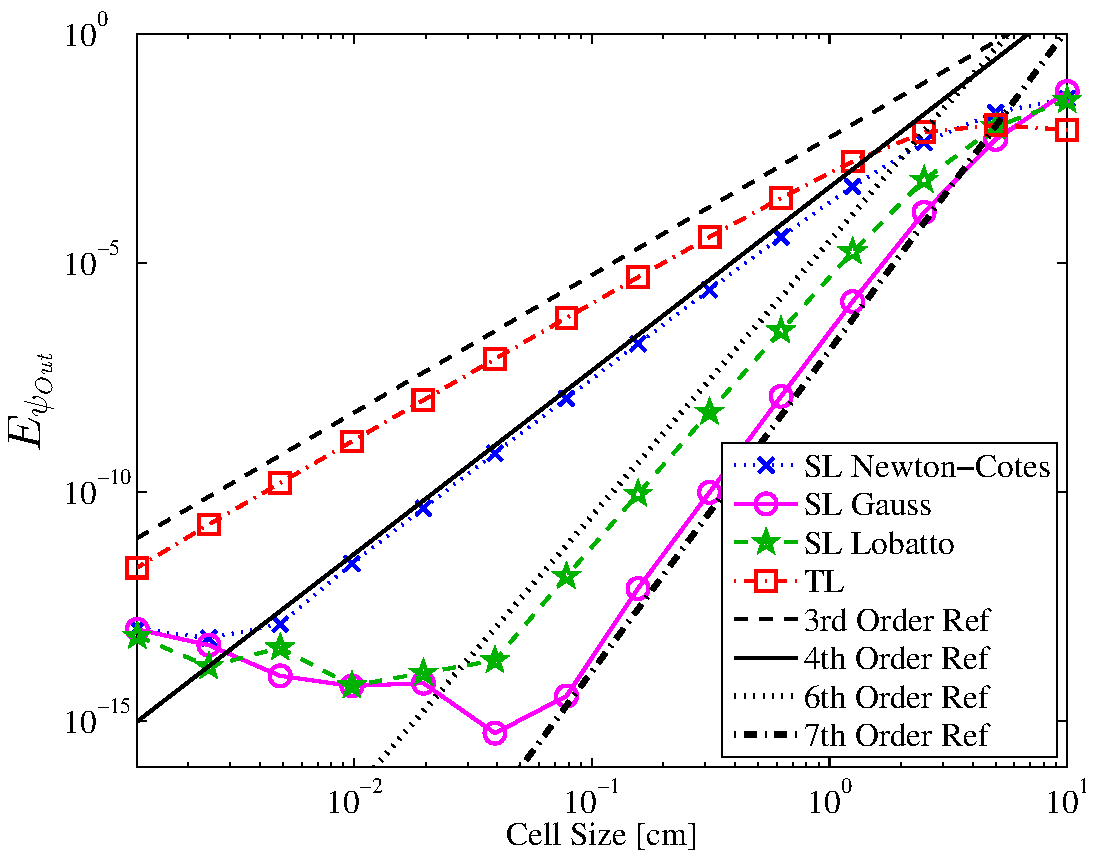
\includegraphics[width=11cm]{chapter2_constant_xs/Cubic_L2Out_err-eps-converted-to.pdf}
\caption{Convergence rate of $E_{\psi,out}$ as a function of the mesh cell size for a homogeneous pure absorber for cubic DFEM.}
\label{fig:multi_L2Out_p3}
\end{figure}
\begin{figure}[!htp]
\centering
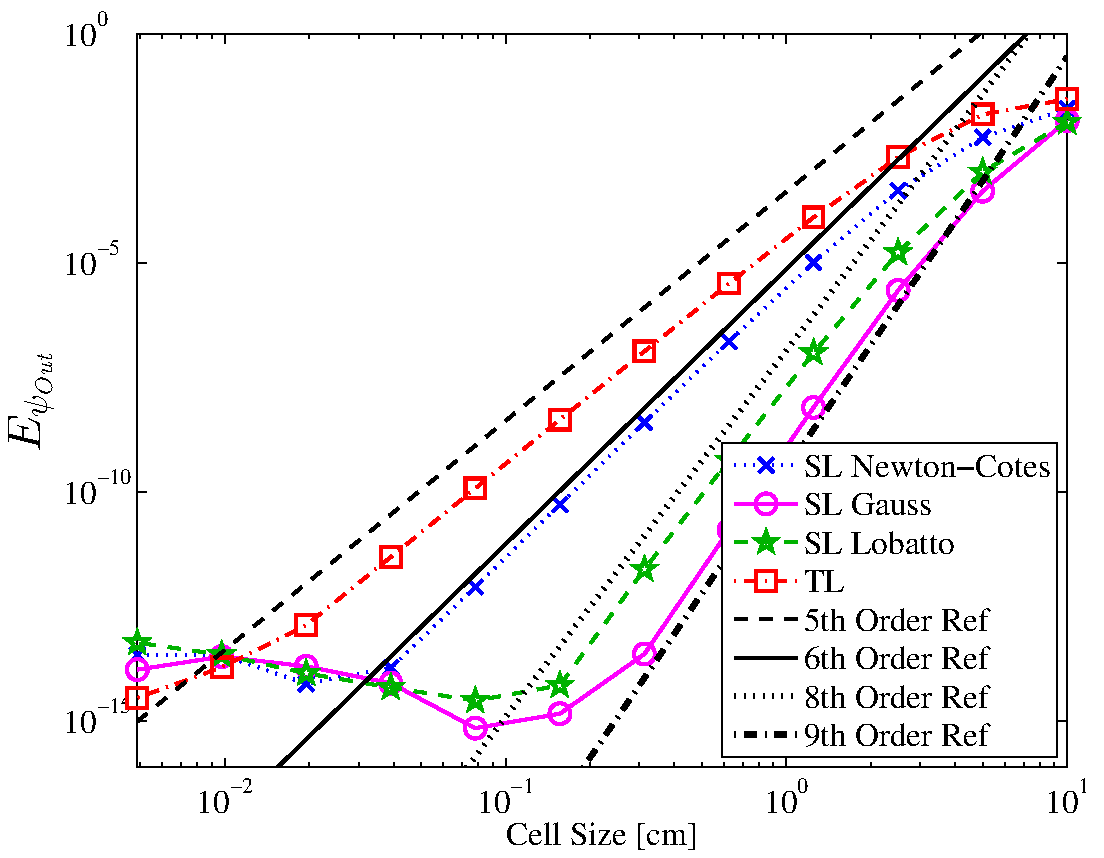
\includegraphics[width=11cm]{chapter2_constant_xs/Quartic_L2Out_err-eps-converted-to.pdf}
\caption{Convergence rate of $E_{\psi,out}$ as a function of the mesh cell size for a pure absorber for quartic DFEM.}
\label{fig:multi_L2Out_p4}
\end{figure}

\pagebreak
The accumulation of errors in multiple-cell problems causes $E_{\psi_{out}}$ to globally converge one order of accuracy lower than the local truncation orders given in \tbl{tbl:taylor_out_part1} and \tbl{tbl:taylor_out_part2}. 
It should be noted that the plateauing of errors $E_{\psi}$, $E_{\psi_A}$, and $E_{\psi_{out}}$ to values $\approx 10^{-14}$ 
in \figs{fig:multi_L2_p1}{fig:multi_L2_p4}, \figs{fig:multi_L2A_p1}{fig:multi_L2A_p4}, and \figs{fig:multi_L2Out_p1}{fig:multi_L2Out_p4}, respectively, is simply a result of our numerical solutions being limited by machine precision (double precision).

%%%%%%%%%%%%%%%%%%%%%%%%%%%%%%%%%%%%%%%%%%%%%%%%%%%%%%%%%%%%%%%%%%
%%%%%%%%%%%%%%%%%%%%%%%%%%%%%%%%%%%%%%%%%%%%%%%%%%%%%%%%%%%%%%%%%%
% \section{Conclusions}
% \label{sec:conclusions}
% %%%%%%%%%%%%%%%%%%%%%%%%%%%%%%%%%%%%%%%%%%%%%%%%%%%%%%%%%%%%%%%%%%
% %%%%%%%%%%%%%%%%%%%%%%%%%%%%%%%%%%%%%%%%%%%%%%%%%%%%%%%%%%%%%%%%%%
% %
% %\marginpar{\textcolor{red}{needs revisions}}
% %
% %\textcolor{red}{first recall what we did: sn transport, DFEM, higher order poly approx, mass lumping strategies}\\

% Lumping methods for arbitrary order DFEM spatial discretizations of the first-order form of the $S_N$ neutron transport equation have been studied in 1-D slab geometry.
% We have analyzed lumping in terms of numerical integration strategy and finite element basis function interpolation point type. Accuracy and robustness of the various
% schemes have been assessed.
% %
% %In particular, we have focused on analyzing numerical schemes (i.e., a combination of integration strategy and finite element basis function interpolation point type) that are both robust and accurate.  
% Robustness is defined in the traditionally accepted assertion in the radiation transport community, i.e., resistance to negative outflow angular flux solutions in source-free pure absorbers with incident angular flux as cell optical thickness is increased.
% Two forms of mass matrix lumping were studied in an attempt to find DFEM discretization schemes that are both robust and yield higher order accuracy with increases in the polynomial degree of the DFEM trial space.  

% The first scheme, traditional mass lumping or TL, exactly integrates the mass matrix and collapses row entries onto the main diagonal to create a diagonal mass matrix.  
% TL yields strictly positive angular flux outflows in a pure absorber with optically thick cells only when utilized with linear DFEM (LDFEM).
% The second form of mass matrix lumping considered here generates a diagonal mass matrix by restricting the DFEM interpolation points to the numerical quadrature points (this automatically generates a diagonal mass matrix).  
% This concept, termed self-lumping or SL, may be new to the radiation transport community but was already presented in \cite{raviart,thomee} in the general context of parabolic equations.
% We have extended these earlier works on self-lumping quadratures by using arbitrary degree polynomial trial spaces and studied three types of interpolation points: 
% (i) equally-spaced points, (ii) Gauss-Legendre quadrature, and (iii) Lobatto-Gauss-Legendre quadrature.  
% Using SL schemes, a strictly positive angular flux outflow can be obtained for all even degree polynomial trial spaces when employing Gauss-Legendre points (SL Gauss).  
% Positive outflow is also obtained for all odd degree polynomial trial spaces using either equally-spaced points (SL Newton-Cotes) or Lobatto-Gauss-Legendre quadratures (SL Lobatto).
% For source driven problems, regardless of mass matrix lumping scheme, it is still possible to obtain negative angular fluxes near cell inflows, for certain source distributions.
% %However, exact integration of fixed source moments will lead to a more robust scheme, regardless of mass matrix lumping strategy. % than if the source moments are approximately evaluated.


% In addition to the robustness of each scheme, we also considered the spatial convergence order of each method for a source-free purely absorbing medium with incident angular flux and constant cross section.  
% The most accurate mass matrix lumping scheme was SL Gauss, for which the average and outflow angular fluxes converged with an order $2P+1$, where $P$ is the polynomial degree of the trial space employed.  
% Since SL Gauss exactly integrates the mass matrix, its behavior is identical to employing exact DFEM, despite having a diagonal mass matrix.  TL was the least accurate of all schemes considered.  
% Increasing the degree of the finite element trial space did not guarantee increased convergence order when using the TL scheme.  
% The SL Newton-Cotes scheme performed better than TL; its order of convergence in the average and outflow angular fluxes increased with an increase in trial space polynomial degree, but in a suboptimal manner.  
% %Further, SL Newton-Cotes, like TL, was at most second order accurate for odd degree polynomial trial spaces and third order accurate for even degree trial spaces in approximating the cell inflow angular flux, respectively.  
% %This lack of local accuracy in calculating $\widetilde{\psi}_{in}$ translated to at most second order convergence for odd degree polynomial trial spaces and third order convergence for even degree polynomial trial spaces in 
% %the $L_2$-norm sense (that is, when calculating $E_{\psi}$).  
% Though not as accurate as SL Gauss for a given degree polynomial trial space, the SL Lobatto scheme only lagged SL Gauss' order of accuracy and spatial convergence by 1 for outflow and cell-averaged quantities.  
% %For all other quantities, SL Lobatto increased two orders of accuracy and spatial order of convergence for each increment in trial space degree, though was always one order less accurate than Exact DFEM and SL Gauss.

% In conclusion, we have shown that, for arbitrary degree polynomial trial space DFEM, a diagonal mass matrix does not necessarily ensure strictly positive angular flux outflow in a purely absorbing slab with spatially constant cross section.  
% Also, we have shown that by using quadrature-based lumping schemes and choosing DFEM interpolation points that are not equally spaced, robust, accurate polynomial DFEM schemes can be obtained.  
% Based on the observed robustness, accuracy, and spatial convergence order results, we conclude that, for applications requiring robust solution techniques, the SL Lobatto scheme with odd degree polynomial trial space DFEM 
% be used to discretize the angular flux .  
% If $p$-adaptivity is desired, software should be developed such that the ability to use either Lobatto (for odd trial space degrees) or Gauss (for even trial space degree) quadrature as the DFEM interpolation points is possible.  
% However, given the non-monotonic behavior of the outflow angular flux as a function of the cell optical thickness when employing the SL Gauss scheme with even degree trial spaces for under-resolved problems, using SL Lobatto 
% with an odd degree trial space would seem to be more accurate than using SL Gauss, despite SL Gauss being more accurate in the asymptotic (fine mesh) limit.

% We see additional opportunities for investigation. % before self-lumping schemes can be used in high order accuracy radiative transfer calculations.
% In particular, we plan on examining the robustness and accuracy of self-lumping DFEM schemes for situations where the cross section is not cell-wise constant.  
% In radiative transfer, the opacity (analog of a cross section) strongly depends on temperature, with temperature varying also within each mesh cell. Thus, opacity is an arbitrary, possibly rapidly, varying function of space.
% The behavior of self-lumping DFEM schemes when cross section is a continuously varying function of space will be of interest in radiative transfer calculations and, as such, should be considered as a topic of research on that subject.

% We also see opportunities to apply self-lumping quadrature to multi-dimensional geometries.  
% While we do not anticipate the multi-dimensional extensions of SL Lobatto or SL Gauss schemes to yield strictly positive angular flux outflows in multi-dimensional geometries, the mass matrix self-lumping technique we have examined here 
% in slab geometry provides a framework not only for mass matrix lumping but also for gradient matrix lumping.
% % in multidimensional geometries.  
% In multi-dimensional problems, mass matrix lumping alone has been shown to be insufficient in preventing solution oscillations. 
% To reduce these oscillations, gradient operator lumping is also required \cite{adams}.
% Though gradient lumping is straightforward on orthogonal grids, it is an open topic of research for non-orthogonal grids \cite{morel_lump}.  Self-lumping methods may provide an adequate framework 
% to carry out consistent mass and gradient lumping on non-orthogonal meshes.


%%%%%%%%%%%%%%%%%%%%%%%%%%%%%%%%%%%%%%%%%%%%%%%%%%%
%
%  New template code for TAMU Theses and Dissertations starting Fall 2012.  
%  For more info about this template or the 
%  TAMU LaTeX User's Group, see http://www.howdy.me/.
%
%  Author: Wendy Lynn Turner 
%	 Version 1.0 
%  Last updated 8/5/2012
%
%%%%%%%%%%%%%%%%%%%%%%%%%%%%%%%%%%%%%%%%%%%%%%%%%%%
%%%%%%%%%%%%%%%%%%%%%%%%%%%%%%%%%%%%%%%%%%%%%%%%%%%%%%%%%%%%%%%%%%%%%%
%%                           SECTION III
%%%%%%%%%%%%%%%%%%%%%%%%%%%%%%%%%%%%%%%%%%%%%%%%%%%%%%%%%%%%%%%%%%%%%



\chapter{\uppercase{DFEM Methods for Neutron Transport for Problems with Spatially Varying Cross Section}}
\label{sec:chapter3_variable_xs}

For many problems of interest to the nuclear science and engineering community, macroscopic cross sections in neutronics and opacities in radiative transfer calculations cannot accurately be described as piecewise constants in space.  
Cross sections and opacities are functions of continuously varying quantities such as temperature, density, burn-up history, etc. \cite{xs_are_T_dependent}.
An examples simulation that is not be adequately described with cell-wise constant cross sections includes nuclear reactor isotopic depletion calculations.
In thermal radiative transfer, interaction opacities can be rapidly varying functions of temperature.  
For example, consider Marshak wave problems and the canonical $T^{-3}$ dependence \cite{ober_shadid} of absorption opacity, 
Across cells near the heated/cold material interface, opacity variations of several orders of magnitude are easily possible.

Historically, the neutron transport and thermal radiative transfer communities assumed interaction cross section and opacities, respectively, that were cell-wise constant \cite{adams,lewis_book,morel_radtran}.
Adams first described \cite{adams_scb} and then presented computational results \cite{adams_nowak} for a ``simple'' corner balance (SCB) spatial discretization method that explicitly accounted for the spatial variation of opacity within individual spatial cells.
The SCB scheme (which can be shown to be related to a LDFEM for certain geometries) accounts for opacity spatial variation within each cell via vertex-based quadrature evaluation.  
Similar strategies have been adapted to LDFEM radiative diffusion \cite{ober_shadid} and LDFEM TRT \cite{warsa_lmfga} calculations.
For accurate TRT solutions, use of higher order DFEM will requires the development of corresponding higher order strategies  for treating the within cell spatial variation of opacities.  
However, the majority of neutron transport literature has only considered the case of cell-wise constant cross sections, see \cite{adams, lewis_book, warsa_krylov, yaqi_ragusa2}. 
The work of Kavenoky and Lautard \cite{varXS_diff} and more recently Santandrea and Bellier \cite{varXS_MOC} are notable exceptions in neutron transport. 
In \cite{varXS_diff}, continuous cubic finite element diffusion calculations that assume a linearly varying spatial cross section within each mesh cell were compared to results obtained using the same spatial discretization but with the assumption that cross sections are constant in each cell.
Similarly, \cite{varXS_MOC} compared the results of a linear characteristic scheme that assumes a linearly varying cross section in each spatial cell 
to those of a linear characteristic scheme that assumes a constant cross section in each cell.

In this chapter, we analyze the effects of cross-section spatial dependence on solution accuracy, as we did in our previously published work in \cite{part_2_paper}.
Our work differs from \cite{varXS_diff,varXS_MOC,adams_scb,adams_nowak} by considering a discontinuous finite element (DFEM) spatial discretization of the slab geometry $S_N$ transport equation using arbitrary degree polynomial finite element trial spaces.  
In addition, like \cite{adams_scb} and \cite{adams_nowak} we do not make any approximation to the particular spatial shape of the cross-section spatial variation in each cell.
We build on the quadrature integration ideas presented in Chapter \ref{sec:chapter2_constant_xs} and employ a numerical quadrature to evaluate the mass matrix integrals that involve cross sections as a function of space.
In general, the quadrature integration of the DFEM interaction term with arbitrary spatial cross section form will not be exact.
However, we showed in Chapter \ref{sec:chapter2_constant_xs} that exact computation of integrals appearing in the DFEM weak form, when cross sections are spatially constant, is not required to achieve high-order accuracy with high-order DFEM approximations.  
Building on this idea, we investigate the effects of using numerical quadratures to compute DFEM mass matrices, accounting for the spatial variation of cross section in space.
As in \secref{sec:chapter2_constant_xs} we use self-lumping numerical quadratures \cite{raviart, thomee}, restricting quadrature integration points to the DFEM polynomial interpolation points.
Results are compared as a function of DFEM polynomial trial space degree and interpolation point type.

We demonstrate that assuming a piecewise constant cross section in each cell, when the cross section is not cell-wise constant in space, has several undesirable effects.  
Considering a source-free, purely absorbing medium, we show that DFEM schemes that assume a cell-wise constant cross section are at most second-order accurate for the angular flux solution and limited to at most first-order accuracy for the interaction rate solution, regardless of the DFEM polynomial trial space degree.  
We also show that assuming a piecewise constant cross section results in a highly discontinuous, non-monotonic spatial interaction rate.  
This phenomena has likely been present in published numerical results for problems with non-piecewise constant cross section but was not observed previously due to the choice of data presentation.

We then consider schemes that explicitly account for cross-section spatial variation within individual mesh cells.
First, the positivity and robustness of different schemes are discussed using a source-free pure absorber problem.
Next, we demonstrate that self-lumping schemes that evaluate the DFEM weak form integrals involving cross section with quadrature 
result in fully accurate schemes for arbitrary degree polynomial DFEM. 
By fully accurate we mean schemes that achieve the same order of convergence for problems with spatially varying and cell-wise constant cross section, for a given DFEM approximation order

%%%%%%%%%%%%%%%%%%%%%%%%%%%%%%%%%%%%%%%%%%%%%%%%%%%%%%%%%%%%%%%%%%%%%
%%%%%%%%%%%%%%%%%%%%%%%%%%%%%%%%%%%%%%%%%%%%%%%%%%%%%%%%%%%%%%%%%%%%%
\section{Weak Form Derivation}
\label{sec:chap3_derive}
%%%%%%%%%%%%%%%%%%%%%%%%%%%%%%%%%%%%%%%%%%%%%%%%%%%%%%%%%%%%%%%%%%%%%
%%%%%%%%%%%%%%%%%%%%%%%%%%%%%%%%%%%%%%%%%%%%%%%%%%%%%%%%%%%%%%%%%%%%%

We begin by repeating the DFEM neutron transport equation derived in Chapter \ref{sec:chapter2_constant_xs}:
\benum
\left( \mu_d \mathbf{G} + \frac{\Sigma_t \Delta x}{2}\mathbf{M} \right) \vec{\psi}_d = \frac{\Delta x}{2}\vec{Q}_d + \mu_d \psi_{in,d} \vec{f} \pep
\label{eq:chap3_start}
\eenum
To account for the within cell variation of cross section, we need only make one change to \eqt{eq:chap3_start}.  We introduce the concept of a reaction matrix, $\mathbf{R}_{\Sigma}$ where $\Sigma$ is any interaction cross section or other material property:
\benum
\label{eq:chap3_mat_form}
\left( \mu_d \mathbf{G} + \frac{\Delta x}{2}\mathbf{R}_{\Sigma_t} \right) \vec{\psi}_d = \frac{\Delta x}{2}\vec{Q}_d + \mu_d \psi_{in,d} \vec{f} \pep
\eenum
The $N_P \times N_P$ reaction matrix, $\mathbf{R}_{\Sigma_t}$ is defined as:
\benum
\mathbf{R}_{\Sigma_t,ij} = \int_{-1}^1{\Sigma_t(s)\B{i}(s)\B{j}(s)~ds} \pep
\label{eq:chap3_react_mat}
\eenum
Note that if $\Sigma_t$ is indeed spatially constant within the mesh cell, there is no approximation in removing $\Sigma_t(s)$ from the integral of \eqt{eq:chap3_react_mat}, giving
\benum
\mathbf{R}_{\Sigma_t,ij} = \Sigma_t \int_{-1}^1{\B{i}(s)\B{j}(s)~ds} \pec
\eenum
which is equivalent to
\benum
\mathbf{R}_{\Sigma_t} = \Sigma_t \mathbf{M} \pep
\eenum

%%%%%%%%%%%%%%%%%%%%%%%%%%%%%%%%%%%%%%%%%%%%%%%%%%%%%%%%%%%%%%%%%%%%%
%%%%%%%%%%%%%%%%%%%%%%%%%%%%%%%%%%%%%%%%%%%%%%%%%%%%%%%%%%%%%%%%%%%%%
\section{Numerical Schemes}
\label{sec:chap3_num_schemes}
%%%%%%%%%%%%%%%%%%%%%%%%%%%%%%%%%%%%%%%%%%%%%%%%%%%%%%%%%%%%%%%%%%%%%
%%%%%%%%%%%%%%%%%%%%%%%%%%%%%%%%%%%%%%%%%%%%%%%%%%%%%%%%%%%%%%%%%%%%%

%We now discuss the different numerical methods considered in this paper.
We consider two classes of numerical methods in this paper.
%, which differ in how they evaluate the integral definitions of$ \mathbf{R}_{\Sigma_t}$, $\mathbf{M}$, and $\mathbf{L}$.  
The first class uses exact spatial integration to evaluate the integrals that define $\mathbf{R}_{\Sigma_t}$.
A second class of methods uses numerical quadrature to evaluate $\mathbf{R}_{\Sigma_t}$, $\mathbf{M}$, and $\mathbf{G}$.  
Specifically, we limit out discussion of quadrature-based integration to so called self-lumping methods \cite{part_1_paper}.  
Self-lumping methods, first discussed in \cite{raviart, thomee} for parabolic problems, use numerical quadrature restricted to the finite element interpolation points, and thus naturally yield diagonal mass matrices.  
A shorthand notation is given in \tbl{tbl:names_chap3} for all of the numerical methods considered in this chapter and described in detail in the remainder of this section.
\begin{table}[!htp]
\centering
\caption{Nomenclature of numerical schemes considered for the pure absorber problem with a spatially exponential cross section.}
\begin{tabular}{|c|c|c|} 
\hline
  Interpolation &   $\mathbf{R}_{\Sigma_t}$ Matrix				& 	Method					\\
  Point Type		&		Integration Strategy														& 	Short Hand Name \\
  \hline
  Equally-  & 		Exact	Integration																	& EXS DFEM \\
  Spaced   	&   using true $\Sigma_t(x)$											&             \\
  \hline
  Equally-  	& 	$\Sigma_t(x) \approx \widehat{\Sigma}_t $,																			& CXS DFEM \\
  Spaced   	&   $\mathbf{R}_{\Sigma_t} \approx \widehat{\Sigma}_t \mathbf{M}$	&             \\
										&		Exact	Integration	of $\mathbf{M}$   																									&							   \\
  \hline
  Equally-  				& Self-Lumping via  												& SLXS Newton-Cotes	 \\
  Spaced   				& Newton-Cotes Quadrature					&																				\\
  {}											&			{} 																							&     																 \\
  \hline
    Lobatto  			& 	Self-Lumping via 		& 	 	SLXS Lobatto \\
  Quadrature 	& Lobatto Quadrature	&	   \\
    {}														&		{}										& 	      \\
  \hline
  Gauss  					& Self-Lumping via  			 	& SLXS Gauss \\
  Quadrature 	& Gauss Quadrature			& 				\\
    {}									&	{}										 								&      \\
  \hline
\end{tabular}
\label{tbl:names_chap3} 
\end{table}

%%%%%%%%%%%%%%%%%%%%%%%%%%%%%%%%%%%%%%%%%%%%%%%%%%%%%%%%%%%%%%%%%%%%%
\subsection{Exact Spatial Integration}
%%%%%%%%%%%%%%%%%%%%%%%%%%%%%%%%%%%%%%%%%%%%%%%%%%%%%%%%%%%%%%%%%%%%%

By exact spatial integration, we mean schemes that compute the entries of  $\mathbf{M}$ and $\mathbf{G}$ exactly. 
Here, we achieve this by using equally-spaced interpolation points and employing a Gauss-Legendre quadrature rule  \cite{abramowitz} that exactly integrates the respective integrands of $\mathbf{M}$ and $\mathbf{G}$.
Two schemes use exact spatial integration.  
One approximates the spatially varying cross section as a cell-wise constant cross section.
The other uses the exact cross section when integrating the weak form DFEM quantities involving cross section.  
The scheme that assumes a cell-wise constant cross section represents the state of the practice in the neutron transport community, while the second scheme represents the ideal scenario for DFEM transport schemes in problems with spatially varying cross sections.

\subsubsection{Exact Cross Section}
%%%%%%%%%%%%%%%%%%%%%%%%%%%%%%%%%%%%%%%%%%%%%%%%%%%%%%%%%%%%%%%%%%%%%

The exact cross section, exact spatial integration scheme (EXS DFEM) attempts to analytically integrate the full definition of  $\mathbf{R}_{\Sigma_t}$.
Note that since $\Sigma_t(x)$ can be an arbitrary function, analytic integration of $\mathbf{R}_{\Sigma_t}$ is in general impossible.  Likewise, quadrature integration is unlikely to be exact.
In our testing of the EXS DFEM scheme, we use a 20-point Gauss-Legendre quadrature to approximately integrate \eqt{eq:chap3_react_mat}.  
Alternatively, adaptive quadrature, with a controllable tolerance, may be used such that the quadrature error in evaluating \eqt{eq:chap3_react_mat} could be reduced below some small tolerance.    

\subsubsection{Constant Cross Section}
%%%%%%%%%%%%%%%%%%%%%%%%%%%%%%%%%%%%%%%%%%%%%%%%%%%%%%%%%%%%%%%%%%%%%

Historically, neutronics and some radiative transfer calculations have approximated spatially varying cross sections by assuming cell-wise constant cross sections \cite{adams, lewis_book, warsa_krylov, morel_radtran}.  
That is, some evaluation of the true $\Sigma_t(s)$ within a given cell is used to determine a constant value, $\hat{\Sigma}_t$, within each cell.  Under this simplification, $\mathbf{R}_{\Sigma_t}$ is approximated as:
\begin{subequations}
\label{eq:chap3_cxs_R}
\benum
%\mathbf{R}_{\Sigma_t,ij} &=& \frac{\hat{\Sigma}_t}{2} \int_{-1}^1{ \B{i}(s) \B{j}(s)~ds} ~~\text{and}\\
\mathbf{R}_{\Sigma_t} = \hat{\Sigma}_t \mathbf{M} \pep 
\eenum
\end{subequations}
In our test problems, the constant cross section scheme (CXS DFEM) uses the volumetric average of $\Sigma_t(s)$ to generate $\hat{\Sigma}_t$:
\benum
\hat{\Sigma}_t = \frac{1}{2}\int_{-1}^1{\Sigma_t(s)~ds} \pep
\label{eq:chap3_cxs_sigma}
\eenum

%%%%%%%%%%%%%%%%%%%%%%%%%%%%%%%%%%%%%%%%%%%%%%%%%%%%%%%%%%%%%%%%%%%%%
\subsection{Self-Lumping Quadrature Integration}
\label{sec:chap3_sl_theory}
%%%%%%%%%%%%%%%%%%%%%%%%%%%%%%%%%%%%%%%%%%%%%%%%%%%%%%%%%%%%%%%%%%%%%

Schemes that are self-lumping evaluate the integrals of \eqt{eq:chap3_react_mat} using numerical quadrature.  In Chapter \ref{sec:chapter2_constant_xs} we showed that by definition, self-lumping schemes create diagonal mass matrices.
Self-lumping schemes also create diagonal reaction matrices:
\benum
\label{eq:chap3_sl_react}
\mathbf{R}_{\Sigma_t,ij} = \left \{ \begin{array}{ll}
w_i \Sigma_t(s_i) ~ & ~ i=j \\
 0 & ~\text{otherwise}
\end{array}
\right. \\
\eenum
Though the choice of interpolation points does not affect exact integration schemes, as shown in Chapter \ref{sec:chapter2_constant_xs}, the choice of interpolation points was shown to influence both the robustness and accuracy of self-lumping schemes.  
We consider equally-spaced closed Newton-Cotes, Lobatto-Gauss-Legendre, and Gauss-Legendre quadratures as interpolation points for self-lumping schemes.
We do not expect any self-lumping scheme to exactly integrate $\mathbf{R}_{\Sigma_t}$, as the integrand defining $\mathbf{R}_{\Sigma_t}$ will generally not be a polynomial.

%%%%%%%%%%%%%%%%%%%%%%%%%%%%%%%%%%%%%%%%%%%%%%%%%%%%%%%%%%%%%%%%%%%%%%
%%%%%%%%%%%%%%%%%%%%%%%%%%%%%%%%%%%%%%%%%%%%%%%%%%%%%%%%%%%%%%%%%%%%%%
\section{Pure Absorber Numerical Results}
\label{sec:chap3_absorber_results}
%%%%%%%%%%%%%%%%%%%%%%%%%%%%%%%%%%%%%%%%%%%%%%%%%%%%%%%%%%%%%%%%%%%%%
%%%%%%%%%%%%%%%%%%%%%%%%%%%%%%%%%%%%%%%%%%%%%%%%%%%%%%%%%%%%%%%%%%%%%

A beam of radiation, $\psi_{in}(\mu_d)$, is incident on the left face of the slab, the right face is a vacuum boundary, $x\in[0, x_R]$, and there are no fixed  volumetric sources in the medium.  
We consider $\Sigma_t(x)$ to be of the form, 
%
%for which the true angular flux solution, $\psi(x,\mu)$, can be calculated.
%%First, we consider $\Sigma_t(x)$ to be a polynomial in $x$:
%%\benum
%%\Sigma_t(x) = d_1 x^{d_2} + d_3 \pec
%%\label{eq:chap3_poly_xs_form}
%%\eenum
%%with constants $d_1~[cm^{-(1+d_2)}],~d_2,~\text{and}~d_3~[cm^{-1}]$.  
%%The analytic solution for a pure absorber with a polynomial total cross section is:
%%\benum
%%\psi(x,\mu) = \left \{
%%\begin{array}{ll}
%%\psi_{in}\exp\left[- \frac{x}{\mu} \left( \frac{ d_1 x^{d_2} }{d_2+1 }- d_3\right) \right] & \mu = \mu_d \\
%%0 & \text{otherwise}
%%\end{array}
%%\right. \pep
%%\label{eq:chap3_polyxs_psi}
%%\eenum
%%By definition, the angular flux outflow, $\psi(x_R,\mu_d)$, is:
%%\benum 
%%\psi_{out} = \psi_{in}\exp\left[- \frac{x_R}{\mu_d} \left( \frac{ d_1 x_R ^{d_2} }{d_2+1 }- d_3\right) \right] \pep
%%\label{eq:chap3_polyxs_psi_out}
%%\eenum
%%
%%We also consider cases where $\Sigma_t(x)$ varies as:
\benum
\Sigma_t(x) = c_1 e^{c_2 x} \pec
\label{eq:chap3_xs_form}
\eenum
with $c_1$ and $c_2$ are constants $[cm^{-1}]$, with $c_1 > 0$ and $c_2\neq 0$.  
The analytic angular flux solution for a source-free pure absorber with an exponentially varying cross section is:
\benum
\psi(x,\mu) = \left \{
\begin{array}{ll}
\psi_{in}(\mu)\exp\left[ \frac{c_1 }{\mu c_2 } \left(1- e^{c_2 x}  \right) \right] & \mu = \mu_d\\
0 & \text{otherwise}
\end{array}
\right. \pep
\label{eq:chap3_exp_psi}
\eenum
By definition, the outflow angular flux from cell $i$, $\psi_{out,i}$ is $\psi(x_{i+1/2},\mu_d)$ and the average angular flux within cell $i$, $\psi_{A,i}$ as
\benum
\label{eq:chap3_psi_a_def}
\psi_{A,i} = \frac{1}{\Delta x_i}\int_{x_{i-1/2}}^{x_{i+1/2}}{\psi(x,\mu_d)~dx} \pec
\eenum
with $\Sigma_t(x)$ defined as in \eqt{eq:chap3_xs_form}. 
The analytical average flux value is:
\benum
\psi_{A,i} = \frac{\psi_{in}(\mu_d)}{\Delta x_i}
\exp\left[\frac{c_1}{\mu_d c_2}  \right] 
\left[E_1\left(\frac{c_1 e^{c_2 x_{i+1/2}}}{\mu_d c_2} \right) - E_1\left(\frac{c_1 e^{c_2 x_{i-1/2}} }{\mu_d c_2} \right)\right] 
\pec
\label{eq:chap3_varxs_A}
\eenum
 with $E_1$ the exponential integral \cite{abramowitz}.
%\benum
%E_1(z) = \int_z^{\infty}{\frac{e^t}{t}~dt} \pep 
%\eenum

%%%%%%%%%%%%%%%%%%%%%%%%%%%%%%%%%%%%%%%%%%%%%%%%%%%%%%%%%%%%%%%%%%%%%%
%\subsection{Single Cell Outflow Comparisons}
%%%%%%%%%%%%%%%%%%%%%%%%%%%%%%%%%%%%%%%%%%%%%%%%%%%%%%%%%%%%%%%%%%%%%%
%
The only variable cross-section schemes that yields strictly positive angular outflows in a source-free pure absorber are the SLXS Lobatto and SLXS Newton-Cotes schemes using a linear trial space.
For $\mu_d > 0$, consider a source-free, purely absorbing cell with known inflow, $\psi_{in}(\mu_d)$, of width $\Delta x$, and the total cross section at each interpolation point is $\Sigma_{t,j}$.
Regardless of the actual functional form of the cross section within the cell, the linear DFEM SLXS Lobatto and SLXS Newton-Cotes schemes'
%(which are equivalent) yield the following $\mathbf{R}_{\Sigma_t}$:
%\benum
%\mathbf{R}_{\Sigma_t} = \left[ \begin{array}{cc} \Sigma_{t,1} & 0 \\ 0 & \Sigma_{t,2} \end{array}\right]\pep
%\eenum
%Solving \eqt{eq:chap3_mat_form}, 
numerical angular flux outflow, $\widetilde{\psi}_d(1)$, is:
\benum
\label{eq:chap3_NC_P1_out}
\widetilde{\psi}_d(1) =  \frac{2\mu_d^2 \psi_{in}(\mu_d)}{2\mu_d^2 + \Delta x^2 \Sigma_{t,1} \Sigma_{t,2} + \Delta x \mu_d \Sigma_{t,1} + \Delta x \mu_d \Sigma_{t,2}}\pep
\eenum
Equation \ref{eq:chap3_NC_P1_out} is strictly positive when $\Sigma_t(x) \geq 0$, suggesting that the strictly positive outflow results observed in \cite{part_1_paper} might hold for an arbitrarily varying spatial cross section.
However, the results of \cite{part_1_paper} do not hold for higher-order DFEM approximations for spatially dependent cross sections.  

%Consider the angular flux outflow of the cubic SLXS Newton-Cotes scheme, which for the case of a cell-wise constant cross section yields strictly positive angular flux outflow:
%Again, regardless of the actual spatial functional form of the cross section, the cubic SLXS Newton-Cotes scheme generates:
%\benum
%\mathbf{R}_{\Sigma_t} = \left[ \begin{array}{cccc}  
%\frac{\Sigma_{t,1}}{4} & 0 & 0 & 0 \\
%0 & \frac{ 3\Sigma_{t,2}}{4} &  0 & 0 \\
%0 & 0 & \frac{3\Sigma_{t,3}}{4} &  0 \\
%0 & 0 & 0 & \frac{\Sigma_{t,4}}{4}  
%\end{array} \right] \pec
%\eenum
%which when used to solve \eqt{eq:chap3_mat_form} yields the following expression for angular flux outflow:
%\benum
%\label{eq:chap3_P3_NC_out}
%\widetilde{\psi}(1) = \frac{32\mu_d^2\psi_{in,d}\left( 27\mu_d^2 + \Delta x^2 \Sigma_{t,2} \Sigma_{t,3} - 6 \Delta x \mu_d \Sigma_{t,2} - 3\Delta x \mu_d \Sigma_{t,3} \right)}
%{\alpha}
%\pec
%\eenum
%and 
%\begin{multline}
%\alpha = 864\mu_d^4 + 108\Delta x\mu_d^3\Sigma_{t,1} + 132\Delta x\mu_d^3\Sigma_{t,2} + 228\Delta x\mu_d^3\Sigma_{t,3} + 108\Delta x\mu_d^3\Sigma_{t,4}  \\
%+ 21\Delta x^2\mu_d^2\Sigma_{t,1}\Sigma_{t,2} + 24\Delta x^2\mu_d^2\Sigma_{t,1}\Sigma_{t,3} + 27\Delta x^2\mu_d^2\Sigma_{t,1}\Sigma_{t,4} + 59\Delta x^2\mu_d^2\Sigma_{t,2}\Sigma_{t,3} \\
%- 24\Delta x^2\mu_d^2\Sigma_{t,2}\Sigma_{t,4} + 69 \Delta x^2 \mu_d^2 \Sigma_{t,3} \Sigma_{t,4} + 10 \Delta x^3 \mu_d \Sigma_{t,1} \Sigma_{t,2} \Sigma_{t,3} - 6 \Delta x^3 \mu_d \Sigma_{t,1} \Sigma_{t,2} \Sigma_{t,4} \\
%+ 6 \Delta x^3 \mu_d \Sigma_{t,1} \Sigma_{t,3} \Sigma_{t,4} + 22 \Delta x^3 \mu_d \Sigma_{t,2} \Sigma_{t,3} \Sigma_{t,4} + 4 \Delta x^4 \Sigma_{t,1} \Sigma_{t,2} \Sigma_{t,3} \Sigma_{t,4})
%\end{multline}
%Obviously, there are combinations of $\Delta x$, $\Sigma_{t,2}$, and $\Sigma_{t,3}$ which can cause the numerator of \eqt{eq:chap3_P3_NC_out} to become negative, resulting in negative angular flux outflows.

To demonstrate that negative cell outflows are possible, we carry out the following test.
In \figs{fig:exp_outflow_p1}{fig:exp_outflow_p4}, we plot the angular flux outflow of each method as a function of trial space degree, and the parameter $c_2$.
We hold the total cell optical thickness to 20 mean-free-path (MFP), vary $c_2 \in [1,10]$, fix $x_R=1$, and $\mu_d =1$.
With an exponential cross section, the cell optical thickness in $MFP$ of a cell  with $x\in[0,x_R]$ is:
\benum
MFP = \int_{0}^{x_R}{\Sigma_t(x)~dx} = \frac{c_1}{c_2}\left( e^{c_2 x_R} - 1 \right) \pep
\label{eq:chap3_mfp_tot} 
\eenum
To maintain a constant optical thickness in \figs{fig:exp_outflow_p1}{fig:exp_outflow_p4}, $c_1$ is required to be:
\benum
c_1 = \frac{c_2~MFP}{e^{c_2 x_R} - 1}\pep
\eenum

\pagebreak
\begin{figure}[!htp]
\centering
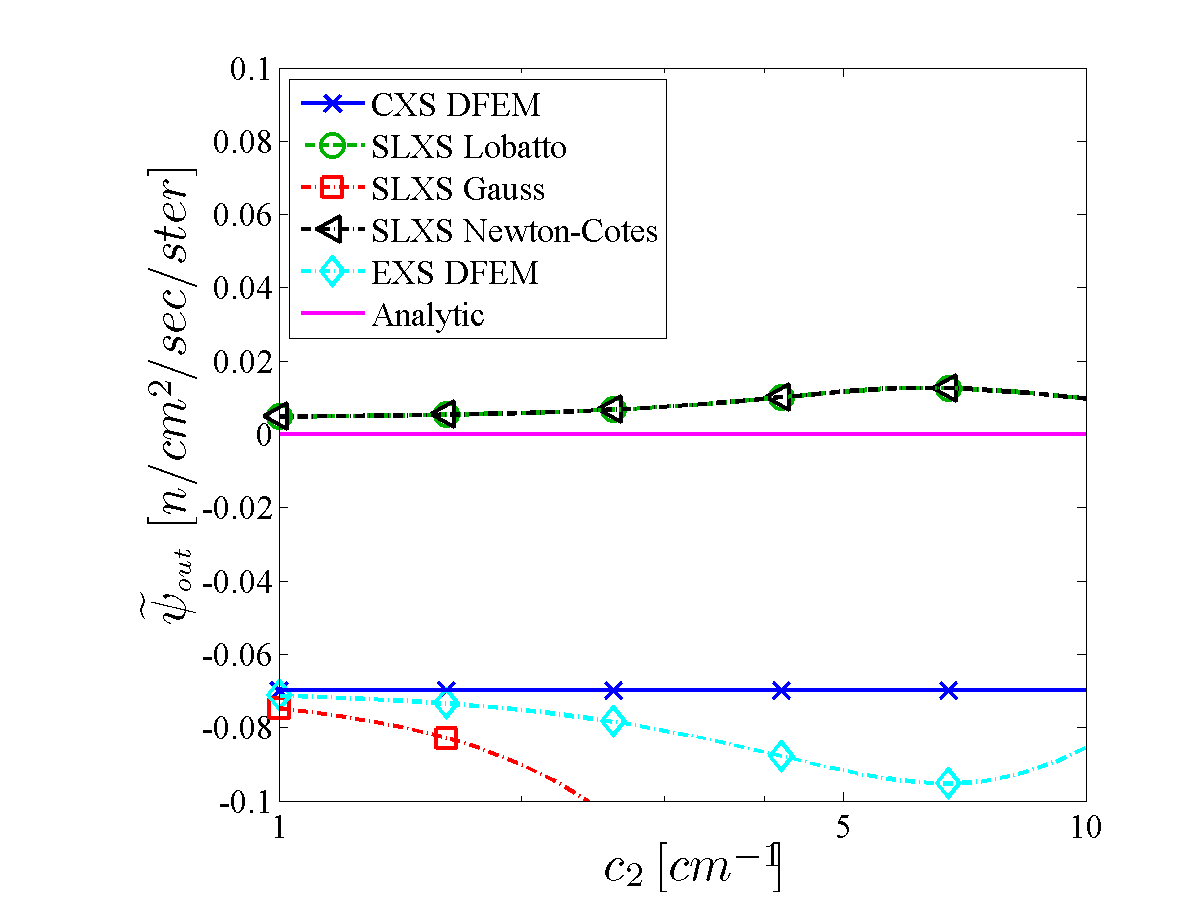
\includegraphics[width=11cm]{chapter3_variable_xs/Exp_outflow_p1.png}
\caption{Numerical outflow from single cell pure absorber with $\Sigma_t(x) = c_1e^{c_2 x}$, as a function of $c_2$ with constant optical thickness of twenty MFP, for a linear trial space.}
\label{fig:exp_outflow_p1}
\end{figure}
%
%
\begin{figure}[!hbp]
\centering
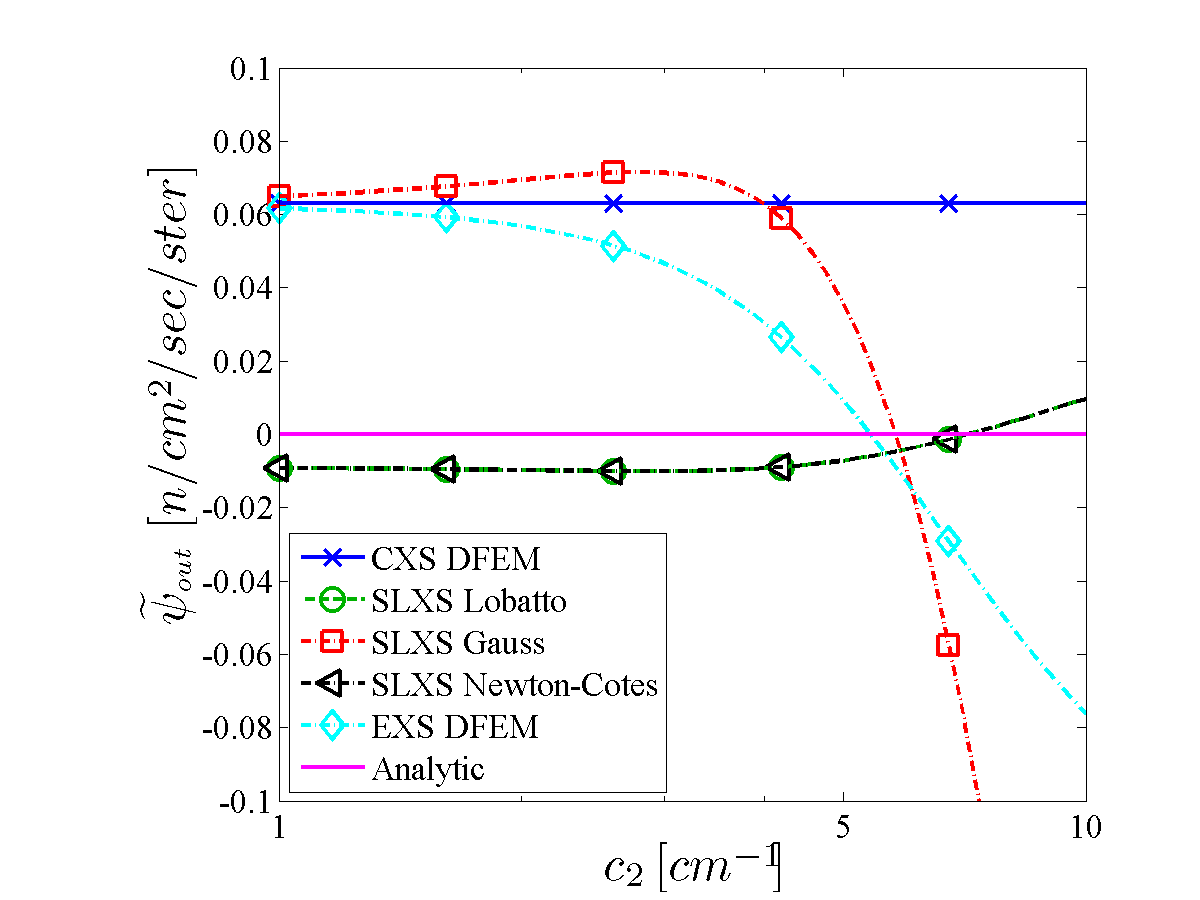
\includegraphics[width=11cm]{chapter3_variable_xs/Exp_outflow_p2.png}
\caption{Numerical outflow from single cell pure absorber with $\Sigma_t(x) = c_1e^{c_2 x}$, as a function of $c_2$ with constant optical thickness of twenty MFP, for a quadratic trial space.}
\label{fig:exp_outflow_p2}
\end{figure}
%
\pagebreak
%
\begin{figure}[!htp]
\centering
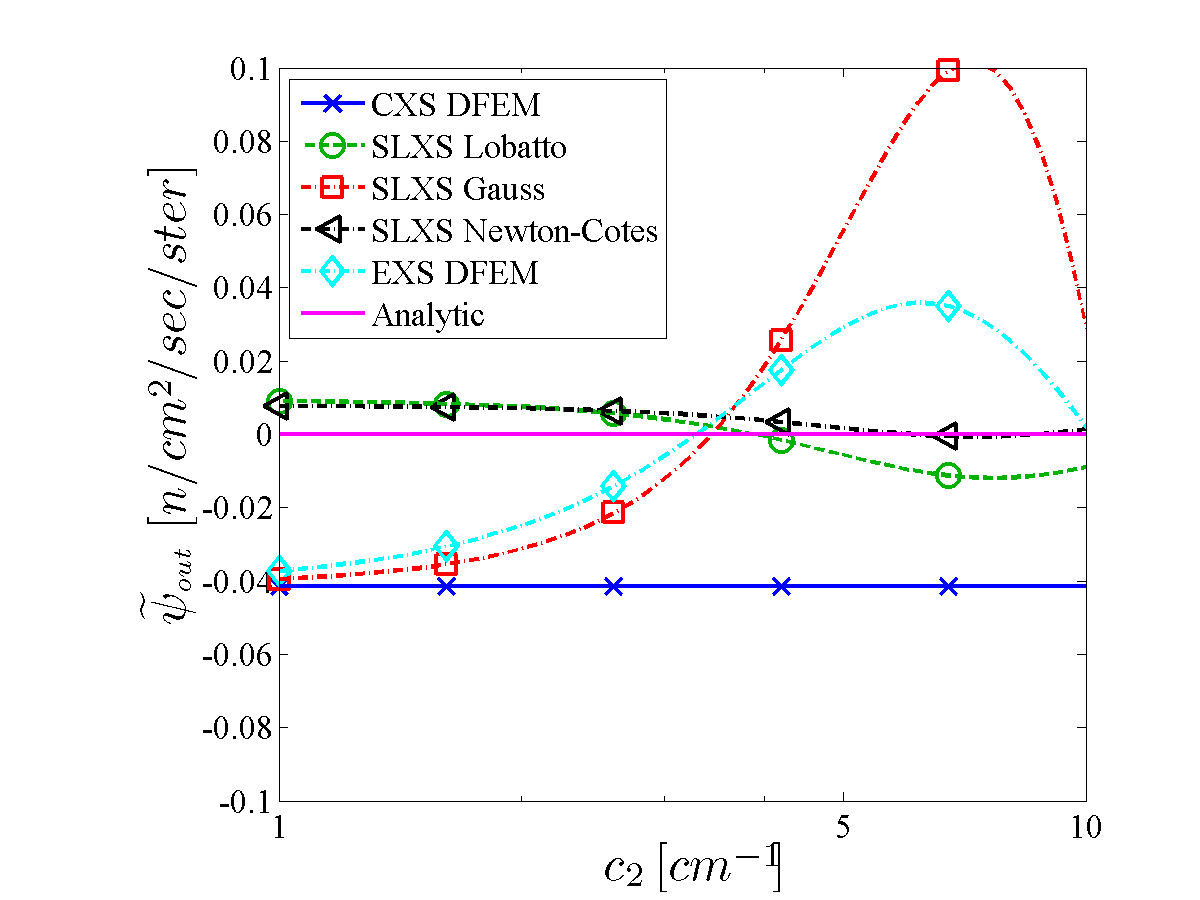
\includegraphics[width=11cm]{chapter3_variable_xs/Exp_outflow_p3.png}
\caption{Numerical outflow from single cell pure absorber with $\Sigma_t(x) = c_1e^{c_2 x}$, as a function of $c_2$ with constant optical thickness of twenty MFP, for different degree polynomial trial spaces.}
\label{fig:exp_outflow_p3}
\end{figure}
%
%
\begin{figure}[!hbp]
\centering
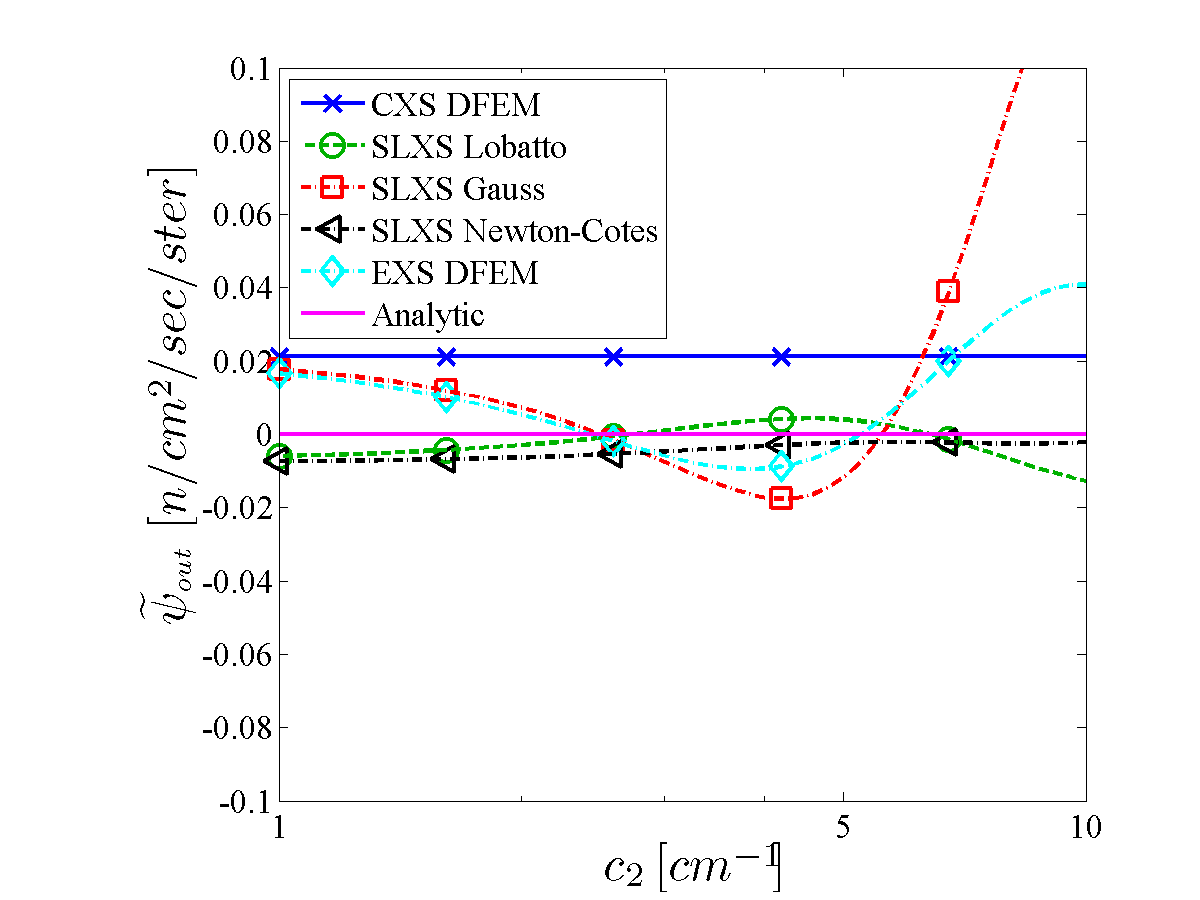
\includegraphics[width=11cm]{chapter3_variable_xs/Exp_outflow_p4.png}
\caption{Numerical outflow from single cell pure absorber with $\Sigma_t(x) = c_1e^{c_2 x}$, as a function of $c_2$ with constant optical thickness of twenty MFP, for different degree polynomial trial spaces.}
\label{fig:exp_outflow_p4}
\end{figure}
\pagebreak

%%In the results that follow, $x_R = 1$, $d_3 = \frac{MFP}{10 x_R}$, and $d_2$ is varied from $[0,10]$.  Results for a cell 1 MFP thick are given in \fig{fig:poly_xs_mfp_1}, for a cell 5 MFP thick in \fig{fig:poly_xs_mfp_5}, and for a cell 10 MFP thick in \fig{fig:poly_xs_mfp_10}.
%%$d_1$ is adjusted to maintain the same number of MFP in each given plot.
%%%  Arranging \eqt{eq:chap3_mfp_tot} $d_1$ will be defined as:
%%%\benum
%%%d_1 = \left(MFP - d_3 x_R \right)\frac{d_2+1}{x_R^{d_2+1}} \pep
%%%\eenum
%%Figures \ref{fig:poly_xs_mfp_1}-\ref{fig:poly_xs_mfp_10} show angular flux outflows as a function of trial space polynomial degree and $d_2$.  As $d_2$ is increased, the spatial variation of $\Sigma_t(x)$ increases.
%%From Figs. \ref{fig:poly_xs_mfp_1}-\ref{fig:poly_xs_mfp_10} it is clear that total cell optical thickness alone does not regulate the positivity of angular flux outflow in a pure absorber with a spatially varying cross section.  
%%
%%
%%The only methods that yield strictly positive angular flux outflow in our testing are CXS DFEM for even degree polynomial trial spaces, and 
%%SLXS Lobatto and SLXS Newton-Cotes for the linear angular flux trial space.  
%%
%%
Figures \ref{fig:exp_outflow_p1}-\ref{fig:exp_outflow_p4} confirms that  SLXS Lobatto (and the equivalent SLXS Newton-Cotes scheme) with a linear trial space is the only scheme that explicitly accounts for the spatial variation of cross and maintains a strictly positive angular flux outflow regardless of the shape of $\Sigma_t(x)$.
From \figs{fig:exp_outflow_p1}{fig:exp_outflow_p4} we also observe that $\widetilde{\psi}_{out}$ varies for every method as a function of the shape of $\Sigma_t(x)$, with the obvious exception of CXS DFEM.
Considering that the analytic angular flux outflow is only a function of total cell MFP:
\benum
\label{eq:chap3_outflow_truth}
\psi_{out,i} = \psi_{in}(\mu_d) \exp\left[-\int_0^{x_{i+1/2}}{\Sigma_t(x)~dx}/ \mu_d \right] = \psi_{in}(\mu_d) \exp\left[-MFP~/\mu_d\right] \pec
\eenum
it is unphysical and undesirable that $\widetilde{\psi}_{out}$, for the SLXS Gauss, SLXS Lobatto, SLXS Newton-Cotes, and EXS DFEM schemes, depends on the spatial shape of $\Sigma_t(x)$.
\clearpage
%%%%%%%%%%%%%%%%%%%%%%%%%%%%%%%%%%%%%%%%%%%%%%%%%%%%%%%%%%%%%%%%%%%%%
\subsection{Multiple Cell Spatial Convergence Rates}
%%%%%%%%%%%%%%%%%%%%%%%%%%%%%%%%%%%%%%%%%%%%%%%%%%%%%%%%%%%%%%%%%%%%%

We now consider the order of spatial convergence for the following schemes: CXS DFEM, SLXS Gauss, SLXS Lobatto, and SLXS Newton-Cotes.  
Since exact integration of $\mathbf{R}_{\Sigma_t}$ is generally not feasible, we no longer consider the EXS DFEM scheme.  
Convergence results of the following angular flux errors as a function of the polynomial approximation order are presented:
\begin{subequations}
\beanum
E_{\psi} &=& \sqrt{\sum_{i=1}^{N_{cells}}{\int_{x_{i-1/2}}^{x_{i+1/2}}{ \left(\widetilde{\psi}_d(x) - \psi(x,\mu_d)  \right)^2  ~dx }}} \\
%E_{\psi_{in}} &=& \sqrt{\sum_{i=1}^{N_{cells}}{\Delta x_i\left(\widetilde{\psi}_{in,i} - \psi(x_{i-1/2})  \right)^2   }}  \\
E_{\psi_A} &=& \sqrt{\sum_{i=1}^{N_{cells}}{\Delta x_i\left(\widetilde{\psi}_{A,i} - \psi_{A,i}  \right)^2   }}  \\
E_{\psi_{out}} &=& \sqrt{\sum_{i=1}^{N_{cells}}{\Delta x_i\left(\widetilde{\psi}_{out,i} - \psi(x_{i+1/2},\mu_d)  \right)^2   }}  \pep
\eeanum
\label{eq:chap3_err_defs}
\end{subequations}
In \eqts{eq:chap3_err_defs}, $\Delta x_i$ is the width of cell $i$, cell $i$ spans $[x_{i-1/2},x_{i+1/2}]$, $\widetilde{\psi}_d(x)$ is the DFEM numerical approximation, $\psi(x,\mu_d)$ is the analytic solution (see \eqt{eq:chap3_exp_psi}).  The problem is spatially discretized using $N_{cells}$ spatial cells of equal width. 
We approximate the integrals defining the $L^2$ norm of the angular flux error, $E_{\psi}$, using a high-order Gauss quadrature set, $(w_{f,q},s_{f,q})$, with $N_{qf}$ points, such that:
\benum
\int_{x_{i-1/2}}^{x_{i+1/2}}{ \left(\widetilde{\psi}(x) - \psi(x,\mu_d)  \right)^2 ~dx}\approx 
\frac{\Delta x_i}{2}\sum_{q=1}^{N_{qf}}{ w_{f,q}\left( \widetilde{\psi}(s_{f,q}) - \psi(s_{f,q},\mu_d)\right)^2 }\pep
\eenum
For the results that follow, $N_{qf} = 10$.
We recall the definitions for the numerical approximations of the cell average angular flux, $\widetilde{\psi}_{A,i}$, and the outflow angular flux, $\widetilde{\psi}_{out,i}$:
\begin{subequations}
\beanum
%\widetilde{\psi}_{in,i} &=& \sum_{j=1}^{N_P}{\psi_{i,j} \B{j}(-1) } \\
\widetilde{\psi}_{A,i} &=& \frac{1}{2}\sum_{j=1}^{N_P}{w_j\psi_{i,j}  } \\
\widetilde{\psi}_{out,i} &=& \sum_{j=1}^{N_P}{\psi_{i,j} \B{j}(1) } \pep
\eeanum
\label{eq:chap3_num_defs}
\end{subequations}

We also consider the convergence of the numerical interaction rate, $\widetilde{IR}(x)$ to the true interaction rate $IR(x)$.  First, we define the analytic reaction rate for our beam problem:
\benum
IR(x) = \Sigma_t(x)\psi(x,\mu_d) \pep
\eenum
Similarly, we define a cell average interaction rate as:
\benum
IR_{A,i} = \frac{1}{\Delta x_i}\int_{x_{i-1/2}}^{x_{i+1/2}}{\Sigma_t(x)\psi(x,\mu_d)~dx} \pep
\eenum
%The numerical approximation to $IR(x)$ depends on the numerical scheme considered.  CXS DFEM is the simplest to consider.  Within cell $i$, CXS DFEM approximates $IR(x)$ as:
%\benum
%\widetilde{IR}(x) = \hat{\Sigma}_{t,i} \widetilde{\psi}(x,\mu_d) \pec
%\label{eq:chap3_cxs_I}
%\eenum
%with a cell average interaction rate approximated as:
%\benum
%\widetilde{IR}_{A,i} = \frac{\hat{\Sigma}_{t,i}}{2} \int_{-1}^1{ \widetilde{\psi}(s,\mu_d)~ds} = \hat{\Sigma}_{t,i} \widetilde{\psi}_{A,i}
%\eenum
Defining a point-wise numerical approximation, $\widetilde{IR}(x)$, to the analytic interaction rate for the self-lumping schemes presents a unique problem, since only a
a numerical quadrature is used to approximate the integrand of $\mathbf{R}$.  
Quadrature integration only requires point evaluations of $\Sigma_t(x)$, not knowledge of $\Sigma_t(x)$ in between quadrature points.
However, for the purpose of plotting the SLXS schemes, we define:
\benum
\widetilde{IR}(s) = \sum_{j=1}^{N_P}{\B{j}(s) \psi_{j,d} \Sigma_t(s_j) } \pep
\label{eq:chap3_sl_lump_inter}
\eenum
%
%It must be emphasized that \eqt{eq:chap3_sl_lump_inter} is only used for plotting purposes.  
%%For other purposes, such as calculating particle conservation, $L^2$ error estimates, etc., using the $\widetilde{IR}(s)$ given in \eqt{eq:chap3_sl_lump_inter} is either invalid or necessitates additional assumptions.
%%such as assuming that $\Sigma_t(x)$ can be approximated as $\widetilde{\Sigma}_t(x)$:
%%\benum
%%\widetilde{\Sigma}_t(s) = \sum_{j=1}^{N_P}{\Sigma_t(s_j) \B{j}(s) } \pep
%%%\eenum
%%With respect to particle conservation, conservation statements must be evaluated with the same integration strategy used in forming the DFEM equations.  
%%An easy way to show this is to consider the CXS DFEM scheme.
%%Calculating the total absorption rate as:
%%\benum
%%\text{Total Absorptions}= \sum_{i=1}^{N_{cells}}{\frac{\Delta x_i}{2}\int_{-1}^1{\Sigma_t(s)\widetilde{\psi}(s,\mu_d) ~ds}} \pec
%%\label{eq:chap3_abs_fake}
%%\eenum
%%using the true, spatially varying $\Sigma_t(s)$, will yield a different total absorption rate than using the cell average cross section method that was used to form the equations:
%%\benum
%%\text{Total Absorptions}= \sum_{i=1}^{N_{cells}}{\frac{\Delta x_i \hat{\Sigma}_{t,i}}{2}\int_{-1}^1{\widetilde{\psi}(s,\mu_d)~ds}} \pep
%%\label{eq:chap3_conserve_cxs}
%%\eenum
%%%Results in a value of $\text{Total Absorption Rates}$ calculated by \eqt{eq:chap3_abs_fake} and \eqt{eq:chap3_conserve_cxs} are different.
%%For \eqt{eq:chap3_abs_fake} and \eqt{eq:chap3_conserve_cxs} to be equivalent, $\Sigma_t(s)$ must be a constant, or $\hat{\Sigma}_{t,i}$ must calculated as in \eqt{eq:chap3_special}:
%%\benum
%%\label{eq:chap3_special}
%%\hat{\Sigma}_{t,i} = \frac{\int_{-1}^1{ \Sigma_t(s) \widetilde{\psi}(s,\mu_d)~ds }}{\int_{-1}^1{\widetilde{\psi}(s,\mu_d)~ds}} \pep
%%\eenum
%%However, calculating $\hat{\Sigma}_{t,i}$ as in \eqt{eq:chap3_special} requires the transport solution to be known first, or requires a non-linear solution process.
We approximate the cell average interaction rate in cell $i$ as:
\benum
\label{eq:chap3_ia_calc}
\widetilde{IR}_{A,i} = \frac{1}{2}\sum_{j=1}^{N_P}{w_j \Sigma_t(s_j) \psi_{j,d} }\pep
\eenum
In \eqt{eq:chap3_ia_calc}, $\Sigma_t(s_j) = \hat{\Sigma}_t$ for the CXS DFEM scheme, and $\Sigma_t(s_j)$ is the point evaluation of the true cross section for all other schemes.

We consider two measures to assess the error of the DFEM schemes' approximation of the true interaction rate, $IR(x)$.  The first, $E_{IR}$ is an approximation of the $L^2$ norm of interaction rate error:
\benum
E_{IR} = \sqrt{
\sum_{i=1}^{N_{cells}}{\frac{\Delta x_i}{2} \sum_{q=1}^{N_P}{w_q \left( IR(s_q) - \Sigma_t(s_q)\widetilde{\psi}(s_q,\mu_d) \right)^2}}
} \pep
\label{eq:chap3_EIR}
\eenum
We reiterate that, for the self-lumping schemes, $\widetilde{IR}(s)$ is only truly defined at the DFEM interpolation points.
%Although less accurate than using a fine quadrature, we evaluate \eqt{eq:chap3_EIR} with quadrature restricted to the DFEM interpolation points, since the self-lumping schemes only conserve particles if $\widetilde{IR}(s)$ is evaluated at the angular flux DFEM interpolation points.
$E_{IR_A}$ measures the convergence of the average interaction rate:
\benum
E_{IR_A} = \sqrt{\sum_{i=1}^{N_{cells}}{\Delta x_i (IR_{A,i} - \widetilde{IR}_{A,i})^2}} \pep
\eenum

For our convergence study, we consider a source-free purely absorbing slab with a cross section that varies exponentially in space as in \eqt{eq:chap3_xs_form} with $c_1 = 0.1$ and $c_2 = 2\ln(10)$.  
A beam of radiation is incident on the left face in the direction of $\mu_d=1$, vacuum boundary conditions exist on the right face of the slab, and $x\in[0, 1]$.  
The convergence of the $E_{\psi}$,  $E_{\psi_A}$, and $E_{\psi_{out}}$ as a function of the choice of numerical scheme for linear through quartic trial space polynomial degree are given in 
\figs{fig:varxs_psi_L2_p1}{fig:varxs_psi_L2_p4},  \figs{fig:varxs_psi_A_p1}{fig:varxs_psi_A_p4}, and \figs{fig:varxs_psi_out_p1}{fig:varxs_psi_out_p4}, respectively.  
\begin{figure}[!htp]
\centering
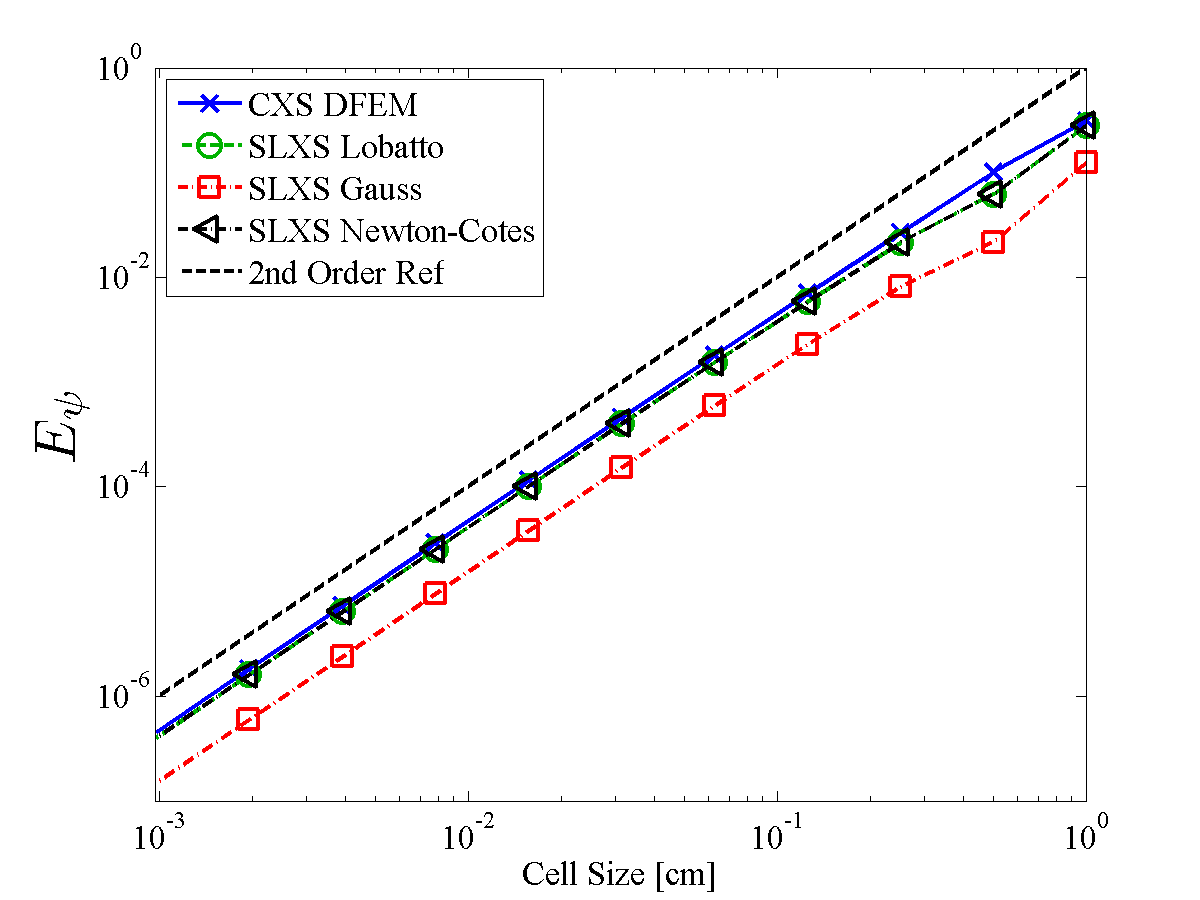
\includegraphics[width=10cm]{chapter3_variable_xs/P1_VarXS_E_psi_L2.png}
\caption{Convergence of $E_{\psi}$ for a pure absorber with exponentially varying cross section discretized with linear DFEM.}
\label{fig:varxs_psi_L2_p1}
\end{figure}
%
%
%
\begin{figure}[!hbp]
\centering
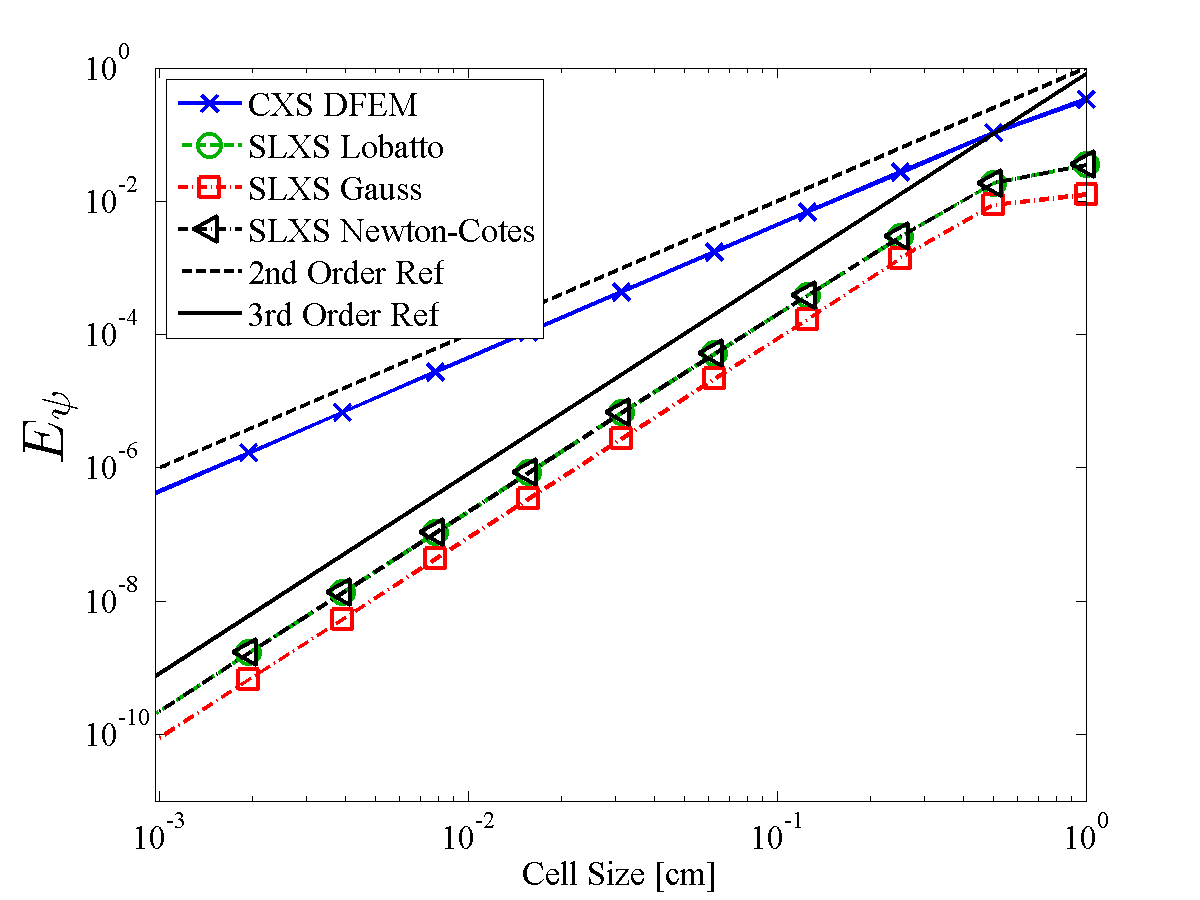
\includegraphics[width=10cm]{chapter3_variable_xs/P2_VarXS_E_psi_L2.png}
\caption{Convergence of $E_{\psi}$ for a pure absorber with exponentially varying cross section discretized with quadratic DFEM.}
\label{fig:varxs_psi_L2_p2}
\end{figure}


\begin{figure}[!htp]
\centering
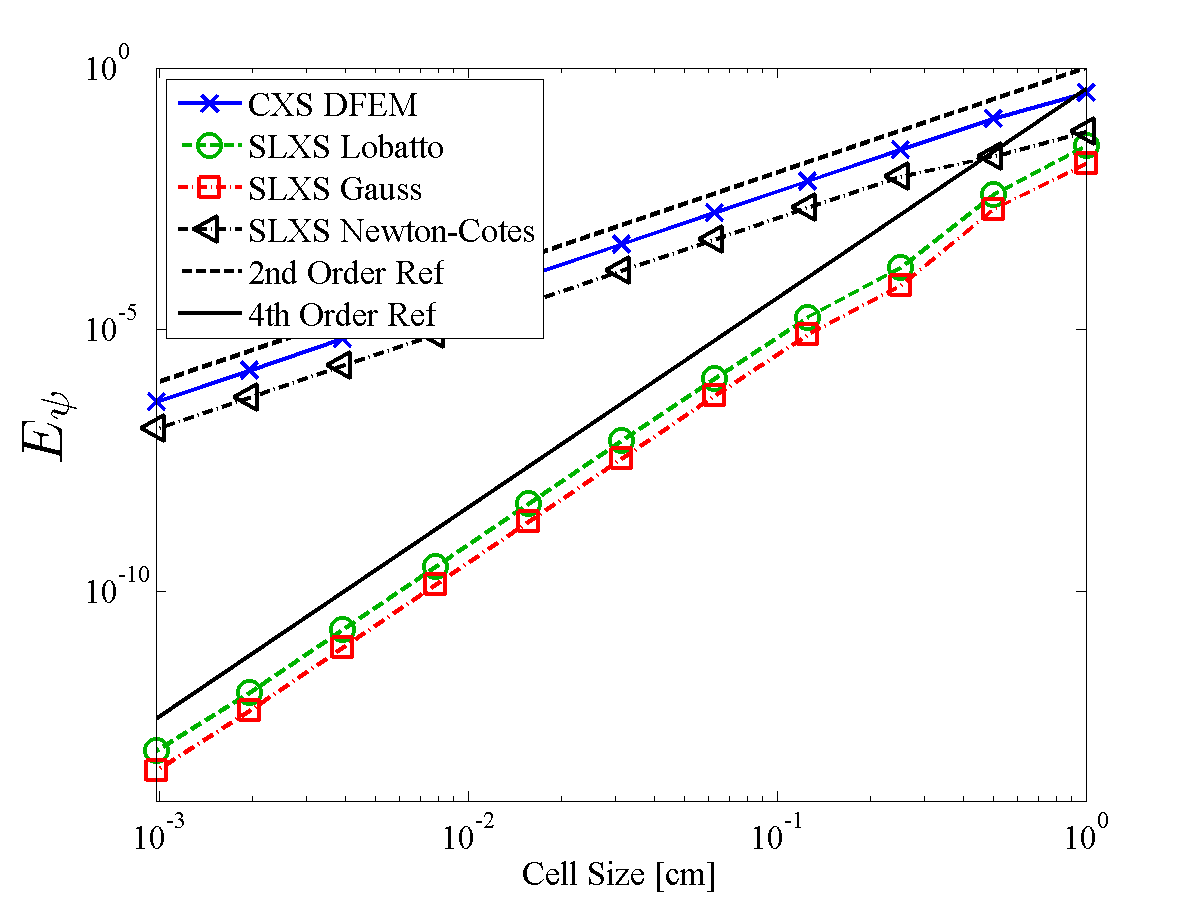
\includegraphics[width=10cm]{chapter3_variable_xs/P3_VarXS_E_psi_L2.png}
\caption{Convergence of $E_{\psi}$ for a pure absorber with exponentially varying cross section discretized with cubic DFEM.}
\label{fig:varxs_psi_L2_p3}
\end{figure}
%
\begin{figure}[!hbp]
\centering
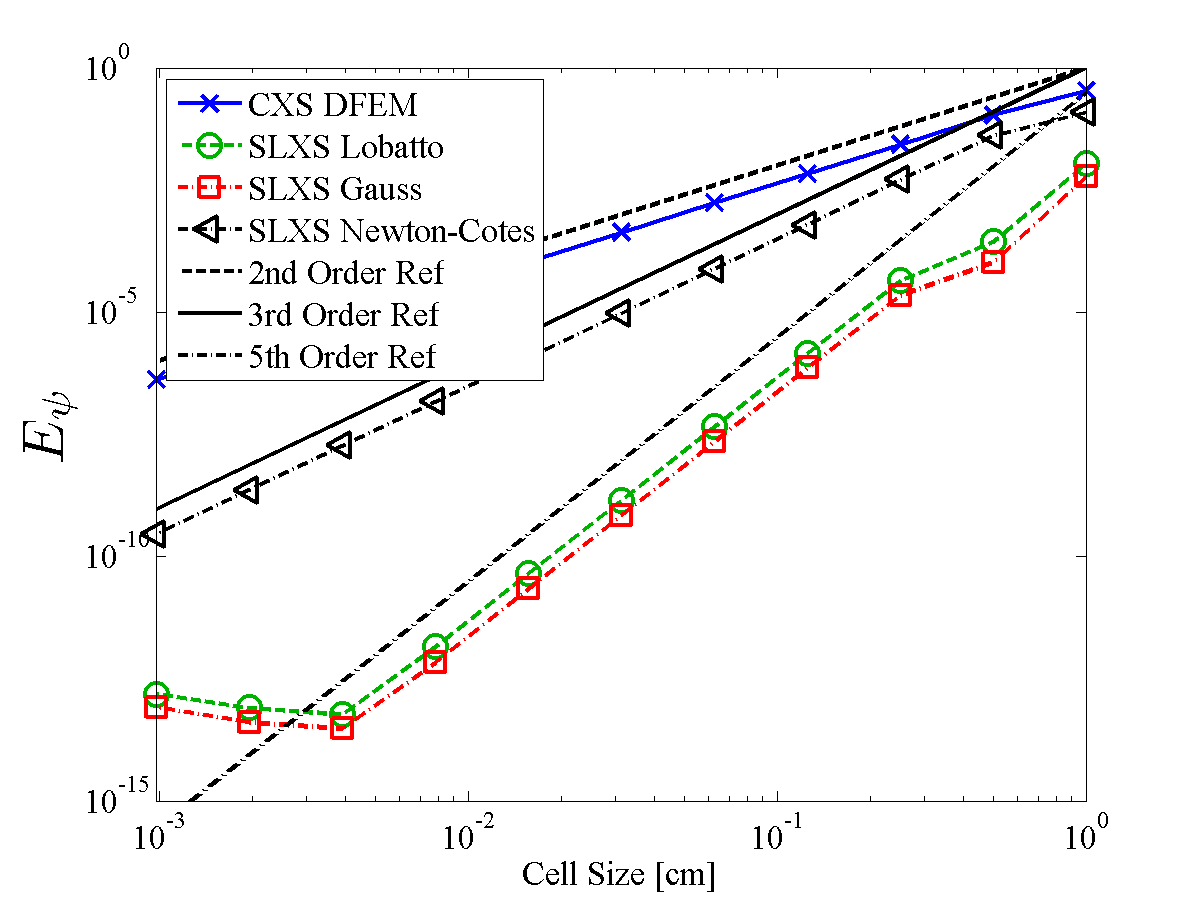
\includegraphics[width=10cm]{chapter3_variable_xs/P4_VarXS_E_psi_L2.png}
\caption{Convergence of $E_{\psi}$ for a pure absorber with exponentially varying cross section discretized with quartic DFEM.}
\label{fig:varxs_psi_L2_p4}
\end{figure}


%
%%
%%
%\begin{figure}[!htp]
%\centering
%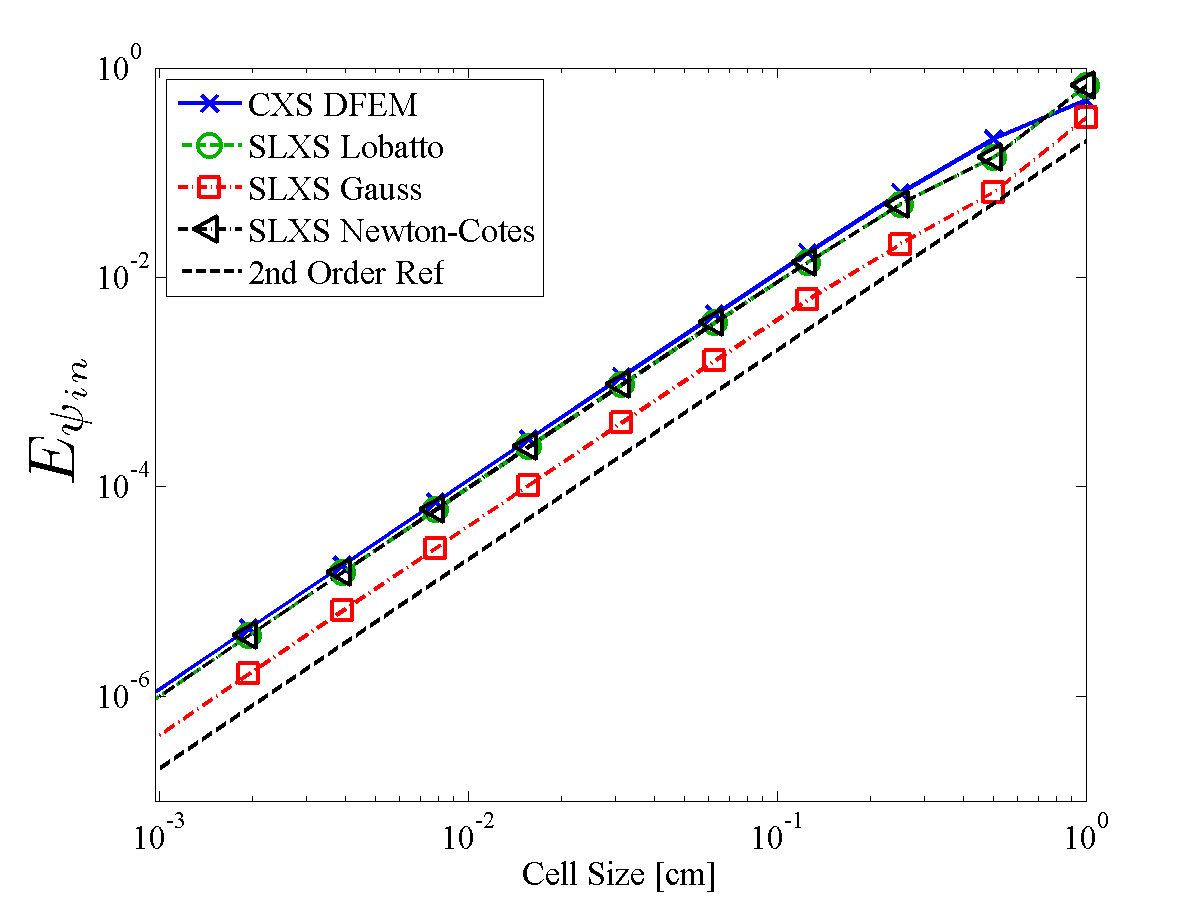
\includegraphics[width=11cm]{chapter3_variable_xs/P1_VarXS_E_psi_in.png}
%\caption{Convergence of $E_{\psi_{in}}$ for a multiple cell problem as a function of cell size for a pure absorber with exponentially varying cross section, $c_3=10$, $c_1 = 0.1~[cm^{-1}]$, $c_2 = 2~[cm^{-1}]$, and $x\in \left[0,1~[cm] \right]$.}
%\label{fig:varxs_psi_in_p1}
%\end{figure}
%%
%%
%\begin{figure}[!htp]
%\centering
%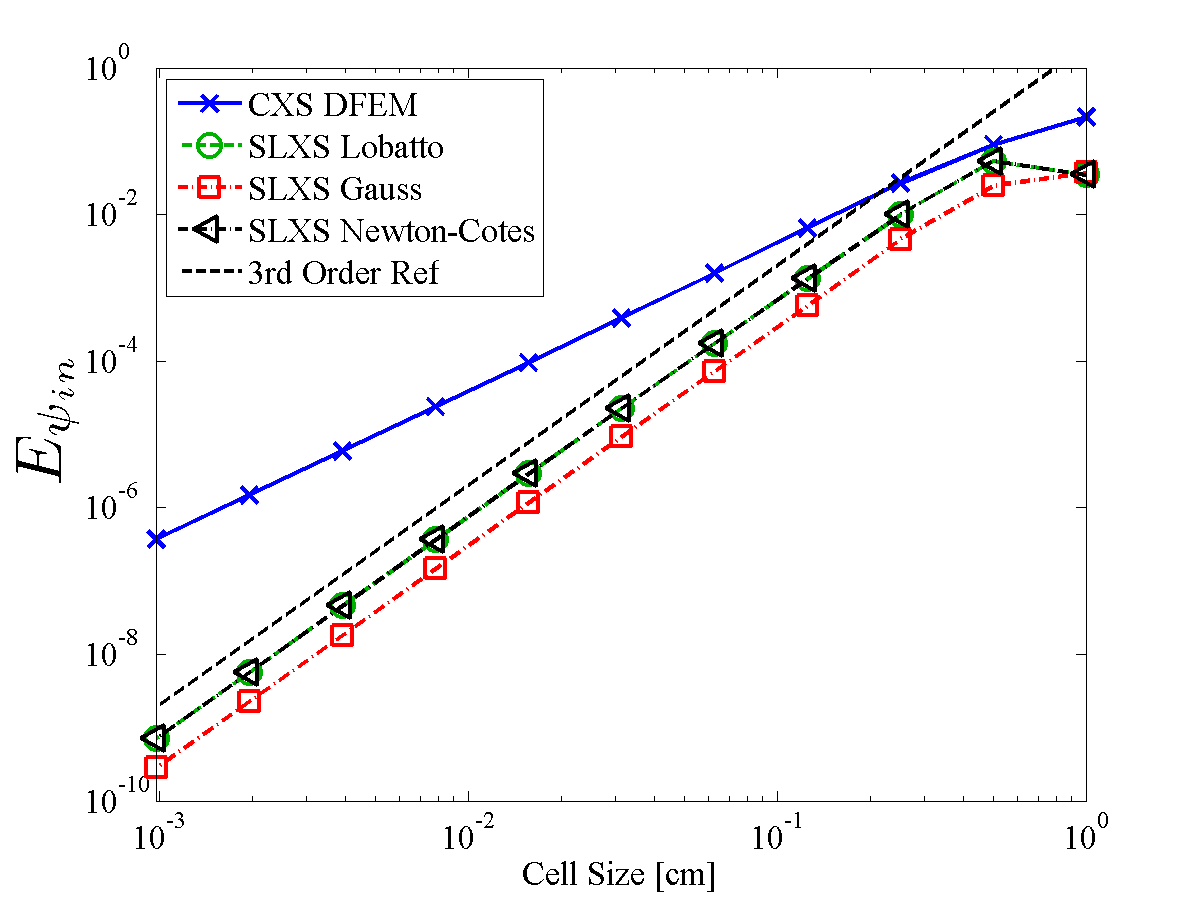
\includegraphics[width=11cm]{chapter3_variable_xs/P2_VarXS_E_psi_in.png}
%\caption{Convergence of $E_{\psi_{in}}$ for a multiple cell problem as a function of cell size for a pure absorber with exponentially varying cross section, $c_3=10$, $c_1 = 0.1~[cm^{-1}]$, $c_2 = 2~[cm^{-1}]$, and $x\in \left[0,1~[cm] \right]$.}
%\label{fig:varxs_psi_in_p2}
%\end{figure}
%%
%%
%\begin{figure}[!htp]
%\centering
%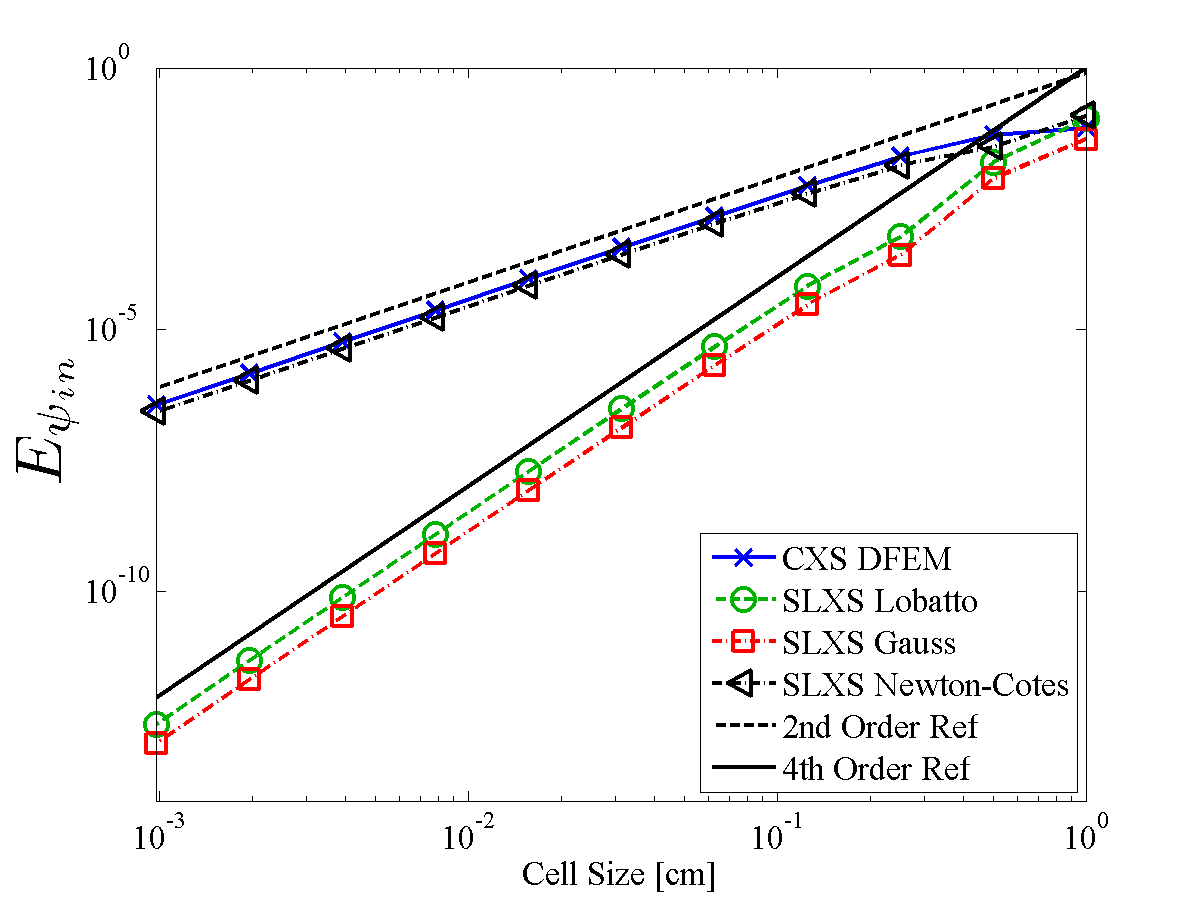
\includegraphics[width=11cm]{chapter3_variable_xs/P3_VarXS_E_psi_in.png}
%\caption{Convergence of $E_{\psi_{in}}$ for a multiple cell problem as a function of cell size for a pure absorber with exponentially varying cross section, $c_3=10$, $c_1 = 0.1~[cm^{-1}]$, $c_2 = 2~[cm^{-1}]$, and $x\in \left[0,1~[cm] \right]$.}
%\label{fig:varxs_psi_in_p3}
%\end{figure}
%%
%%
%\begin{figure}[!htp]
%\centering
%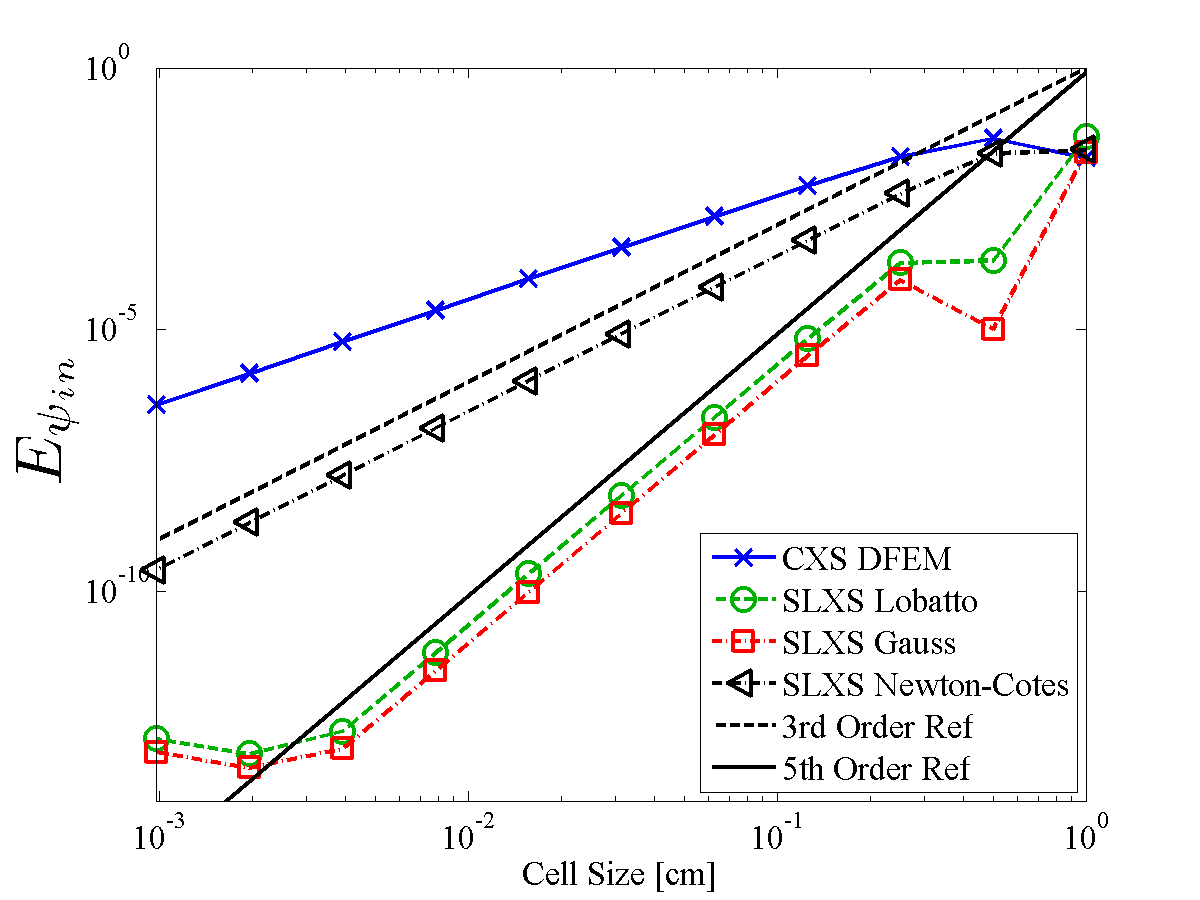
\includegraphics[width=11cm]{chapter3_variable_xs/P4_VarXS_E_psi_in.png}
%\caption{Convergence of $E_{\psi_{in}}$ for a multiple cell problem as a function of cell size for a pure absorber with exponentially varying cross section, $c_3=10$, $c_1 = 0.1~[cm^{-1}]$, $c_2 = 2~[cm^{-1}]$, and $x\in \left[0,1~[cm] \right]$.}
%\label{fig:varxs_psi_in_p4}
%\end{figure}
%%
%%
%%

\begin{figure}[!htp]
\centering
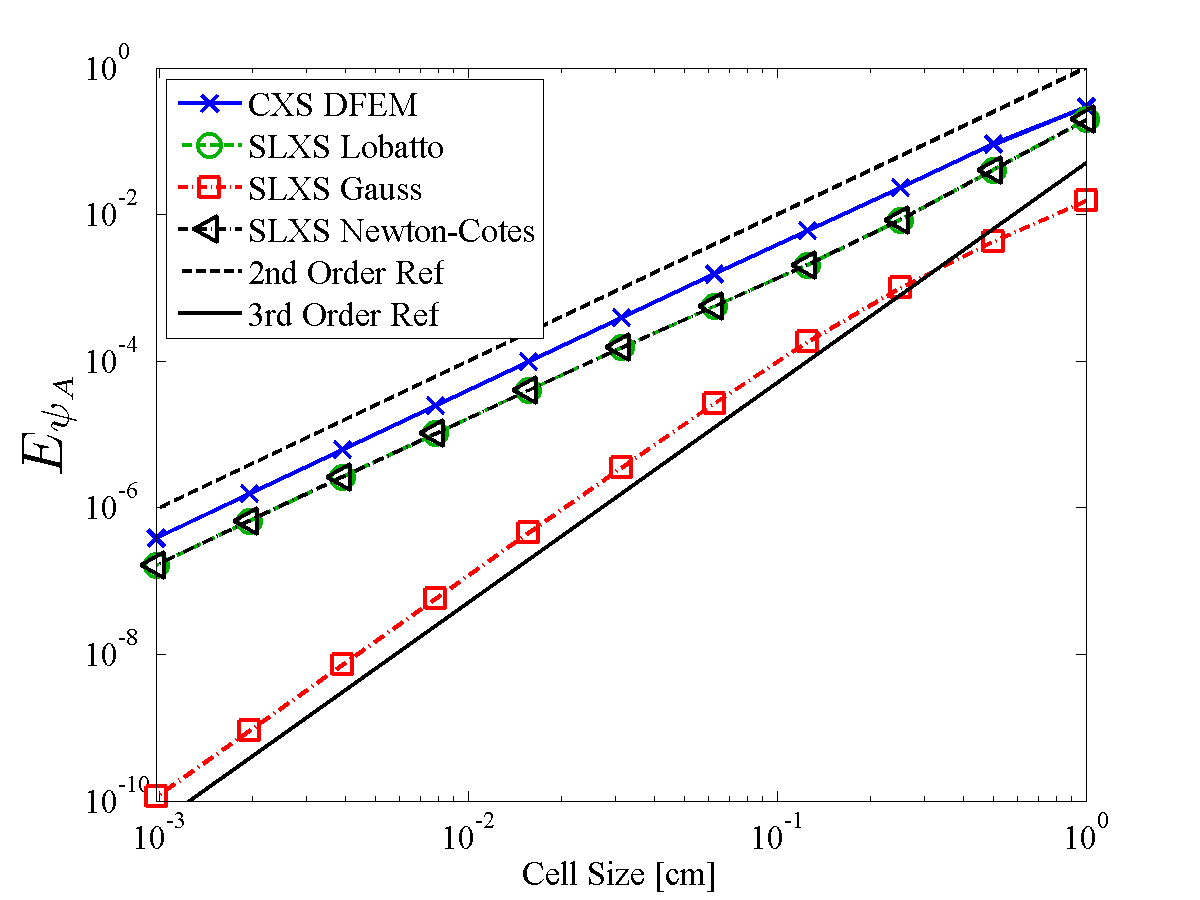
\includegraphics[width=10cm]{chapter3_variable_xs/P1_VarXS_E_psi_A.png}
\caption{Convergence of $E_{\psi_A}$  for a pure absorber with exponentially varying cross section discretized with linear DFEM.}
\label{fig:varxs_psi_A_p1}
\end{figure}
%
\begin{figure}[!hbp]
\centering
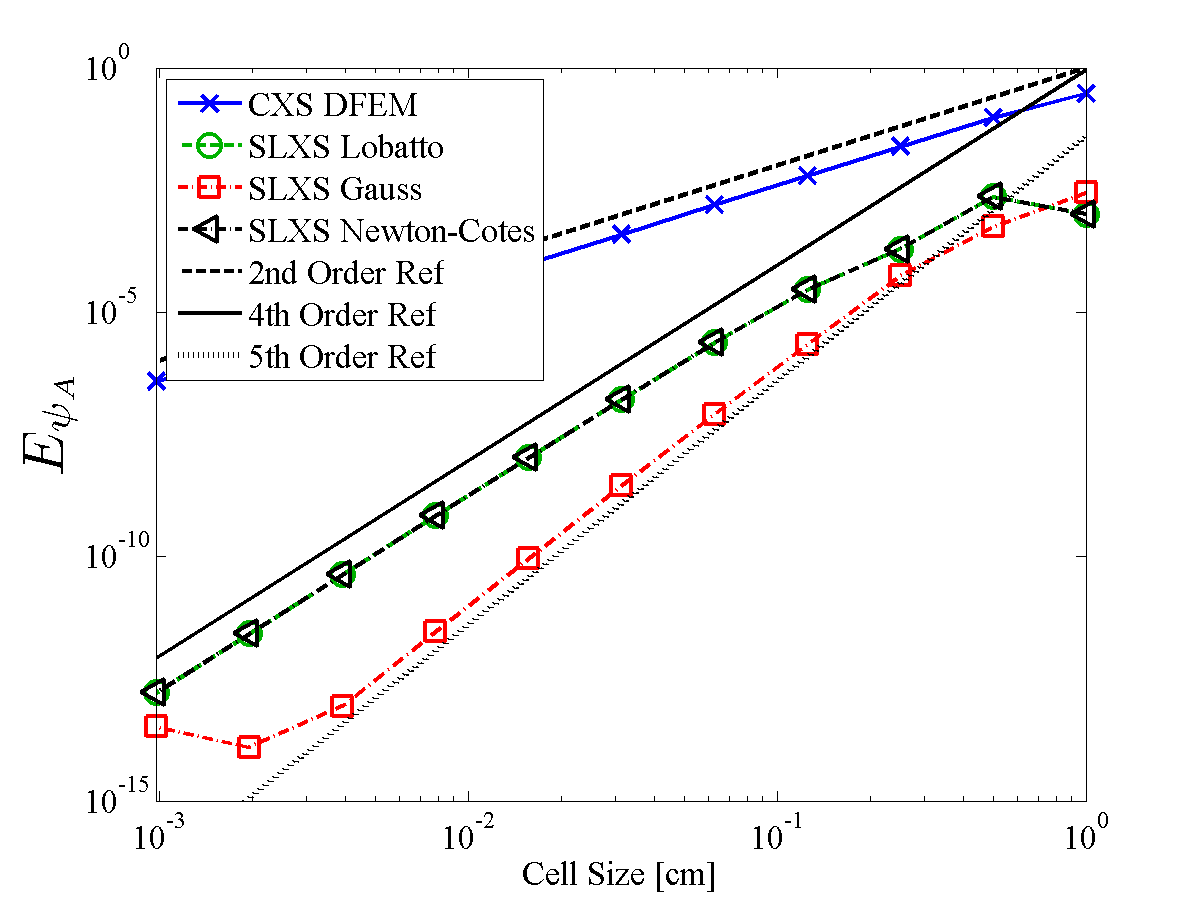
\includegraphics[width=10cm]{chapter3_variable_xs/P2_VarXS_E_psi_A.png}
\caption{Convergence of $E_{\psi_A}$ for a pure absorber with exponentially varying cross section discretized with quadratic DFEM.}
\label{fig:varxs_psi_A_p2}
\end{figure}
%


%
\begin{figure}[!htp]
\centering
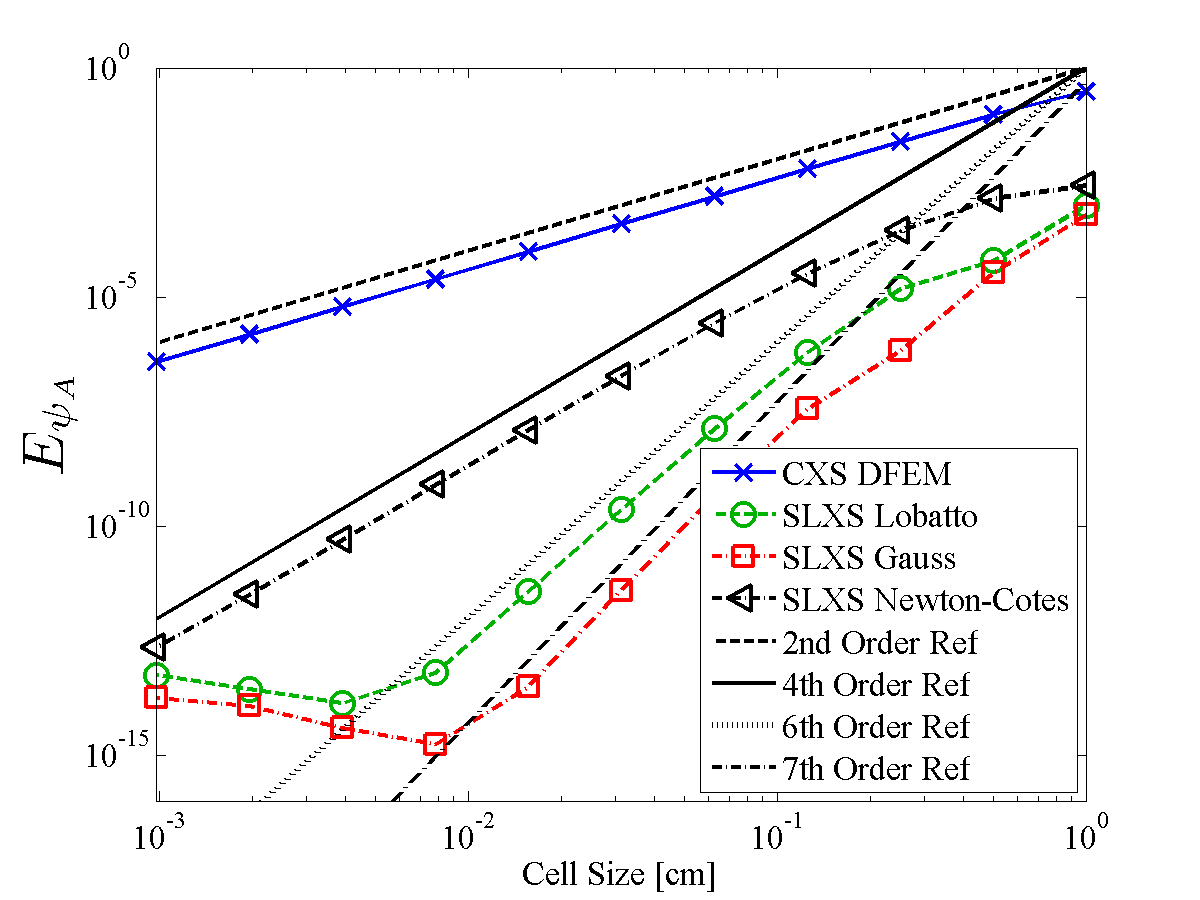
\includegraphics[width=10cm]{chapter3_variable_xs/P3_VarXS_E_psi_A.png}
\caption{Convergence of $E_{\psi_A}$  for a pure absorber with exponentially varying cross section discretized with cubic DFEM.}
\label{fig:varxs_psi_A_p3}
\end{figure}
%
%
\begin{figure}[!hbp]
\centering
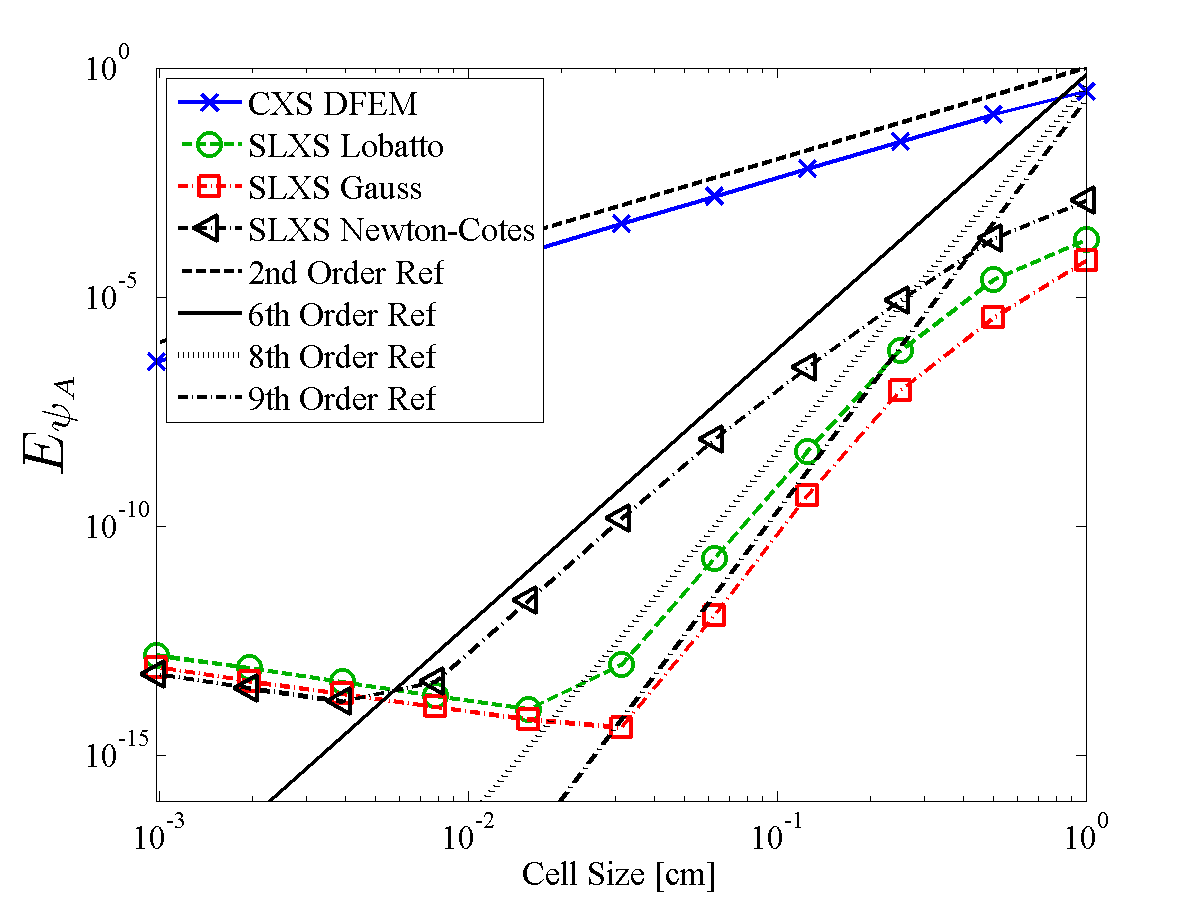
\includegraphics[width=10cm]{chapter3_variable_xs/P4_VarXS_E_psi_A.png}
\caption{Convergence of $E_{\psi_A}$  for a pure absorber with exponentially varying cross section discretized with quartic DFEM.}
\label{fig:varxs_psi_A_p4}
\end{figure}
%


%
\begin{figure}[!htp]
\centering
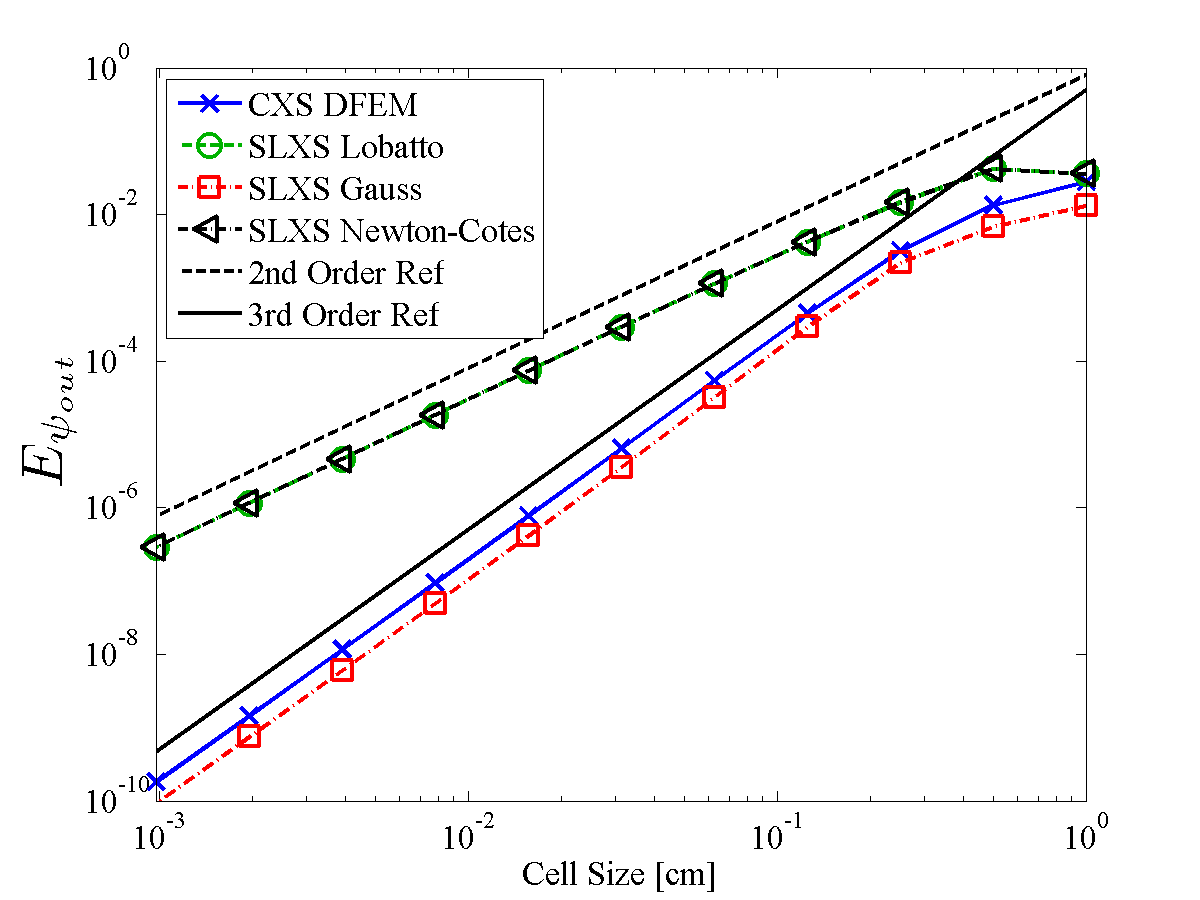
\includegraphics[width=10cm]{chapter3_variable_xs/P1_VarXS_E_psi_out.png}
\caption{Convergence of $E_{\psi_{out}}$  for a pure absorber with exponentially varying cross section discretized with linear DFEM.}
\label{fig:varxs_psi_out_p1}
\end{figure}
%
%
\begin{figure}[!hbp]
\centering
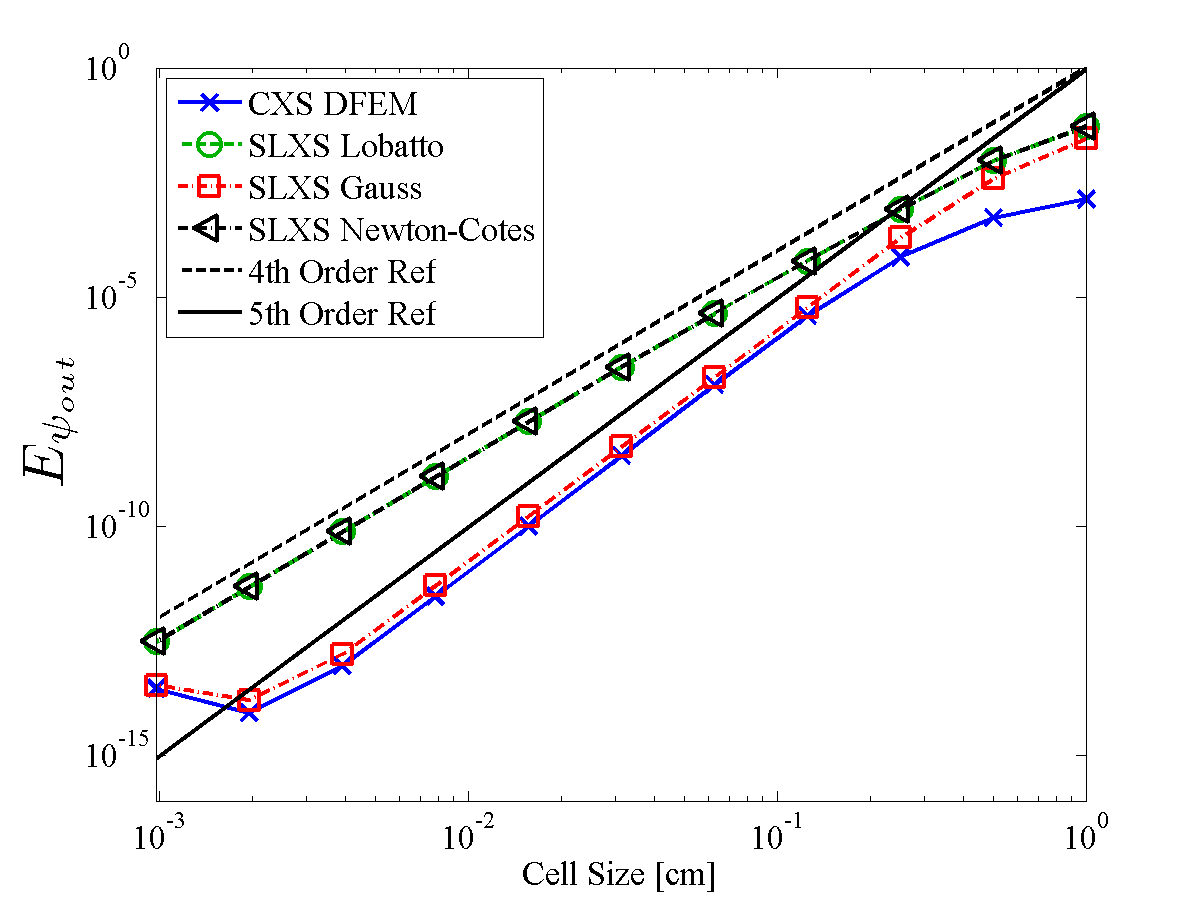
\includegraphics[width=10cm]{chapter3_variable_xs/P2_VarXS_E_psi_out.png}
\caption{Convergence of $E_{\psi_{out}}$  for a pure absorber with exponentially varying cross section discretized with quadratic DFEM.}
\label{fig:varxs_psi_out_p2}
\end{figure}
%



%
\begin{figure}[!htp]
\centering
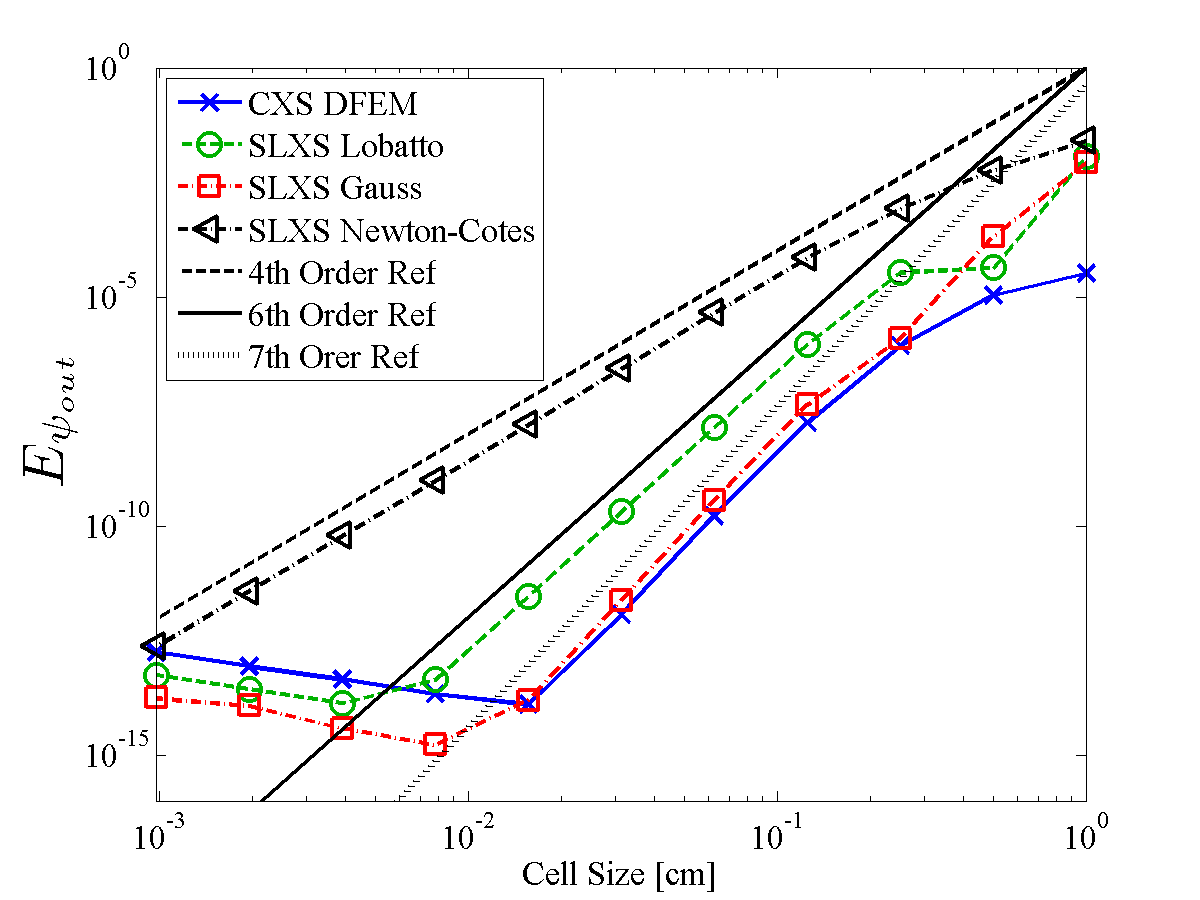
\includegraphics[width=10cm]{chapter3_variable_xs/P3_VarXS_E_psi_out.png}
\caption{Convergence of $E_{\psi_{out}}$  for a pure absorber with exponentially varying cross section discretized with cubic DFEM.}
\label{fig:varxs_psi_out_p3}
\end{figure}
%
\begin{figure}[!hbp]
\centering
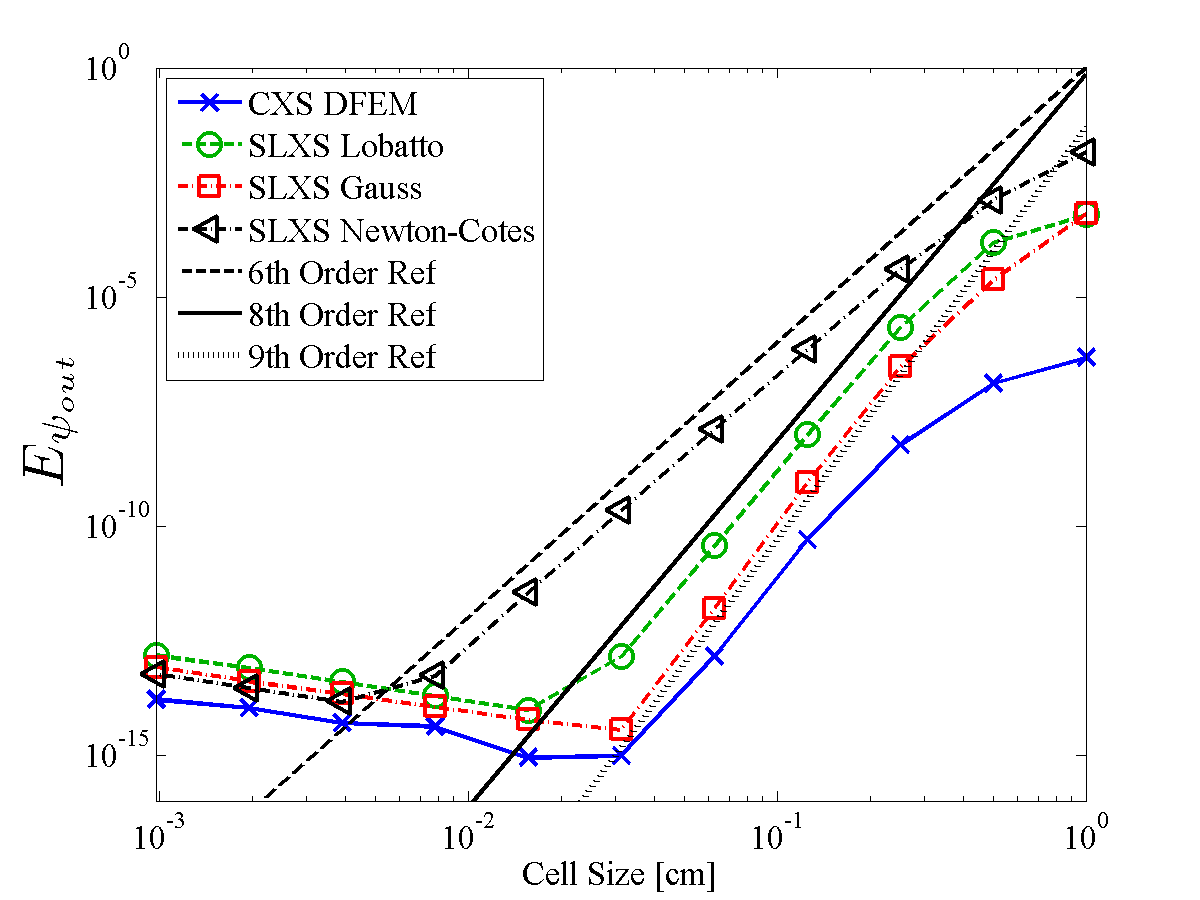
\includegraphics[width=10cm]{chapter3_variable_xs/P4_VarXS_E_psi_out.png}
\caption{Convergence of $E_{\psi_{out}}$  for a pure absorber with exponentially varying cross section discretized with quartic DFEM.}
\label{fig:varxs_psi_out_p4}
\end{figure}
%%
\clearpage
%%
The plateauing of numerical errors for various high-order methods using very small cell sizes in Figs. \ref{fig:varxs_psi_L2_p1}-\ref{fig:varxs_psi_out_p4} is a consequence of having  reached machine precision.
The lines in Figs. \ref{fig:varxs_psi_L2_p1}-\ref{fig:varxs_psi_out_p4} that extend to values smaller than machine precision are reference lines.

Figures \ref{fig:varxs_psi_L2_p1}-\ref{fig:varxs_psi_out_p4} show that, for a linear angular flux trial space, CXS DFEM achieves the same orders of spatial convergence as observed with Exact DFEM in \cite{part_1_paper}.
However, as the degree of the DFEM trial space is increased, the CXS DFEM scheme does not show an increase in the order of the spatial convergence rate of  $E_{\psi}$ and $E_{\psi_A}$; the convergence rate of CXS DFEM is limited to at most second order for both $E_{\psi}$ and $E_{\psi_A}$, regardless of the trial space polynomial degree.  
The increase in order of convergence of CXS DFEM for $E_{\psi_{out}}$ as trial space is increased is a result of angular flux outflow in the
CXS DFEM discretization being only a function of the cell optical thickness, which is preserved exactly by our definition of $\hat{\Sigma}_t$; see \eqt{eq:chap3_cxs_sigma}.

Of the self-lumping schemes, SLXS Newton-Cotes is the least accurate.  SLXS Newton-Cotes convergence of $E_{\psi}$ is limited to at most second order for odd degree polynomial trial spaces and third order for even degree trial spaces.  
Convergence of $E_{\psi_A}$ and $E_{\psi_{out}}$ for the SLXS Newton-Cotes scheme generally increases with an increase in the DFEM polynomial trial space degree, but is only proportional to $P$.
Both SLXS Lobatto and SLXS Gauss converge $E_{\psi}$, $E_{\psi_A}$, and $E_{\psi_{out}}$ similarly to the study carried out in \cite{part_1_paper} with a spatially constant cross section.

The spatial convergence of $E_{\psi}$ for SLXS Lobatto and SLXS Gauss is order $P+1$.
Though SLXS Lobatto and SLXS Gauss converge with the same order of spatial convergence for $E_{\psi}$, SLXS Gauss is more accurate than SLXS Lobatto by a constant.  
SLXS Gauss converges $E_{\psi_A}$ and $E_{\psi_{out}}$ $\propto 2P+1$, whereas SLXS Lobatto converges both $\propto 2P$.
SLXS Gauss and SLXS Lobatto converge angular flux error quantities for the case of a spatially varying cross section with the same rates of convergence as their constant cross-section analogs did in \cite{part_1_paper}.
This suggests that exactly integrating the interaction term in the DFEM moment equations is not essential for developing arbitrarily high-order accuracy DFEM schemes for radiation transport.

Convergence of $E_{IR}$ as function of numerical scheme for linear - quartic trial spaces is given in \figs{fig:varxs_I_L2_p1}{fig:varxs_I_L2_p4}.
%
%
\begin{figure}[!hbp]
\centering
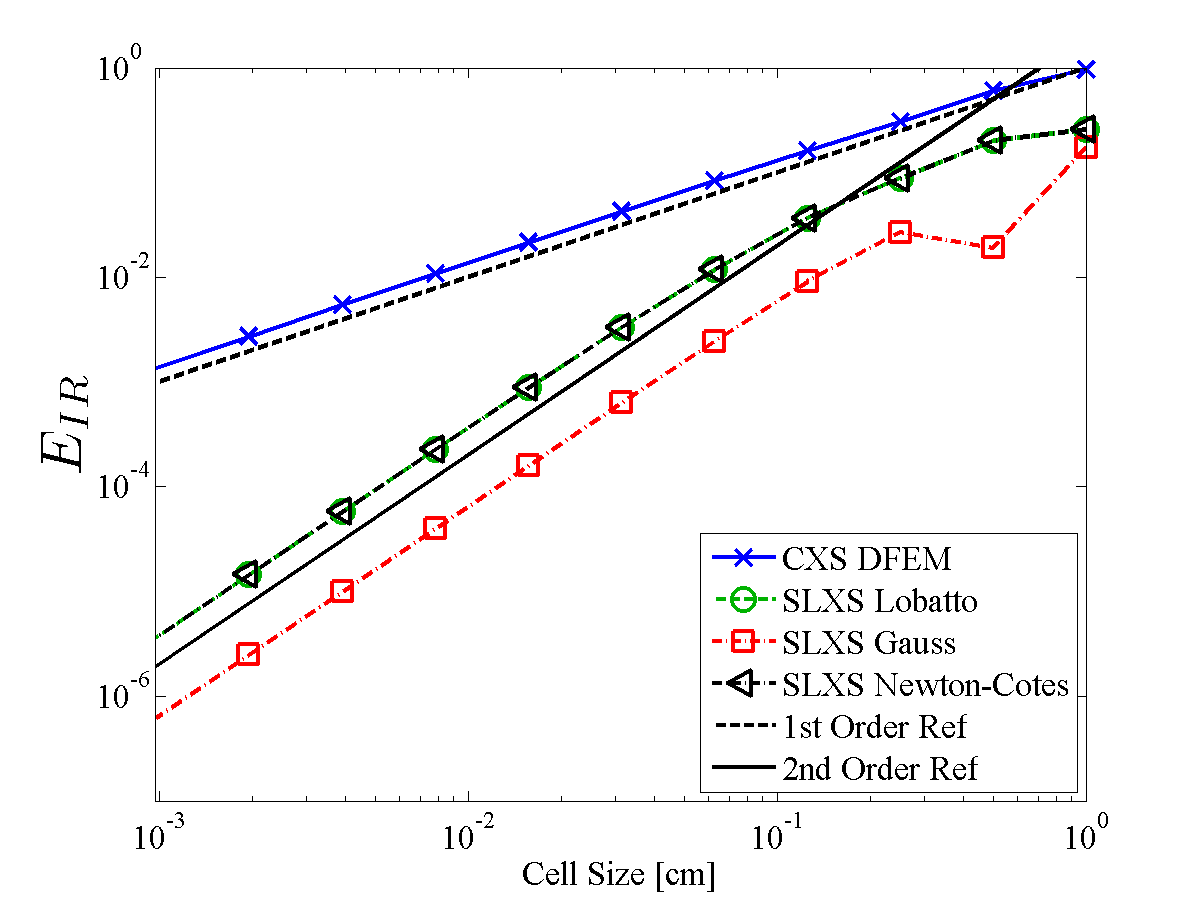
\includegraphics[width=10cm]{chapter3_variable_xs/P1_VarXS_E_I_L2.png}
\caption{Convergence of $E_{IR}$ for a pure absorber with exponentially varying cross section discretized with linear DFEM.}
\label{fig:varxs_I_L2_p1}
\end{figure}
%
%
\begin{figure}[!htp]
\centering
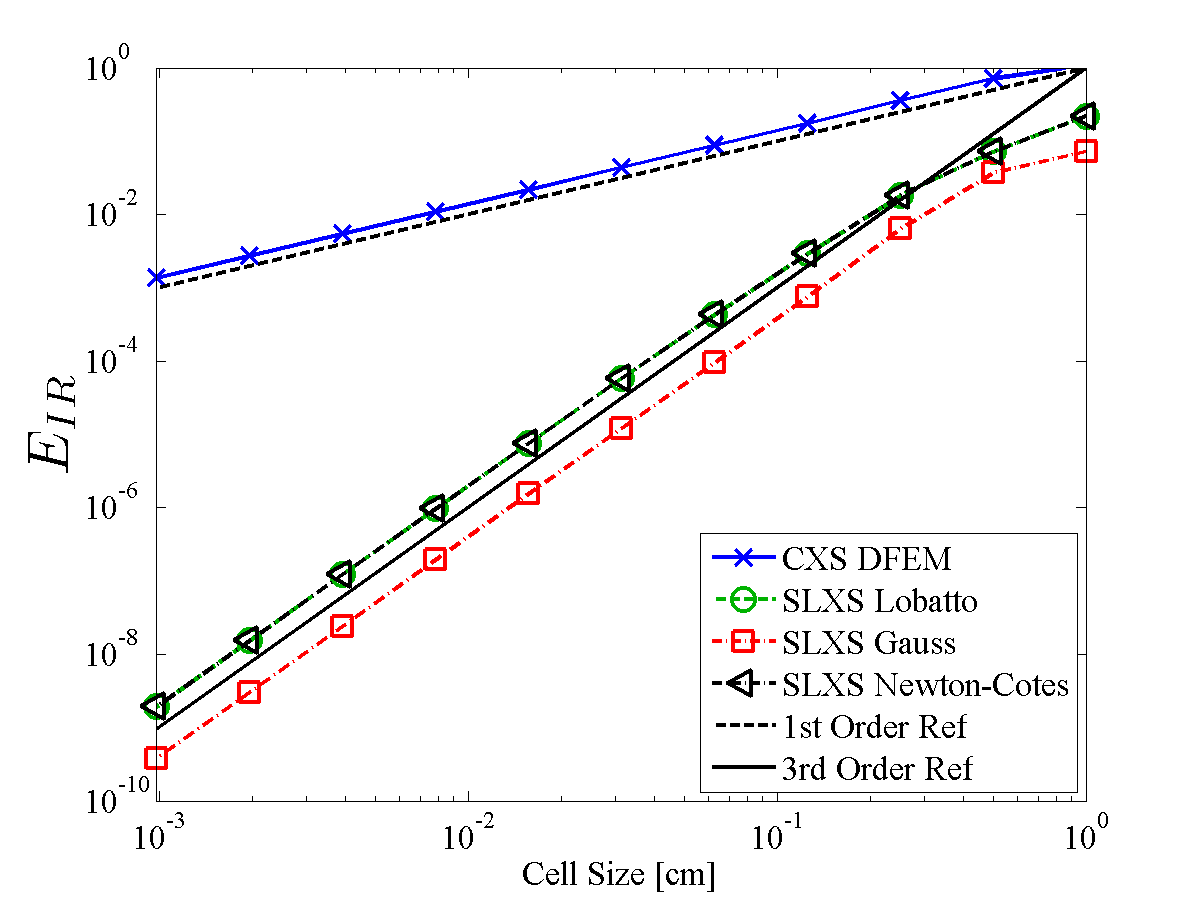
\includegraphics[width=10cm]{chapter3_variable_xs/P2_VarXS_E_I_L2.png}
\caption{Convergence of $E_{IR}$ for a pure absorber with exponentially varying cross section discretized with quadratic DFEM.}
\label{fig:varxs_I_L2_p2}
\end{figure}
%
%
\begin{figure}[!hbp]
\centering
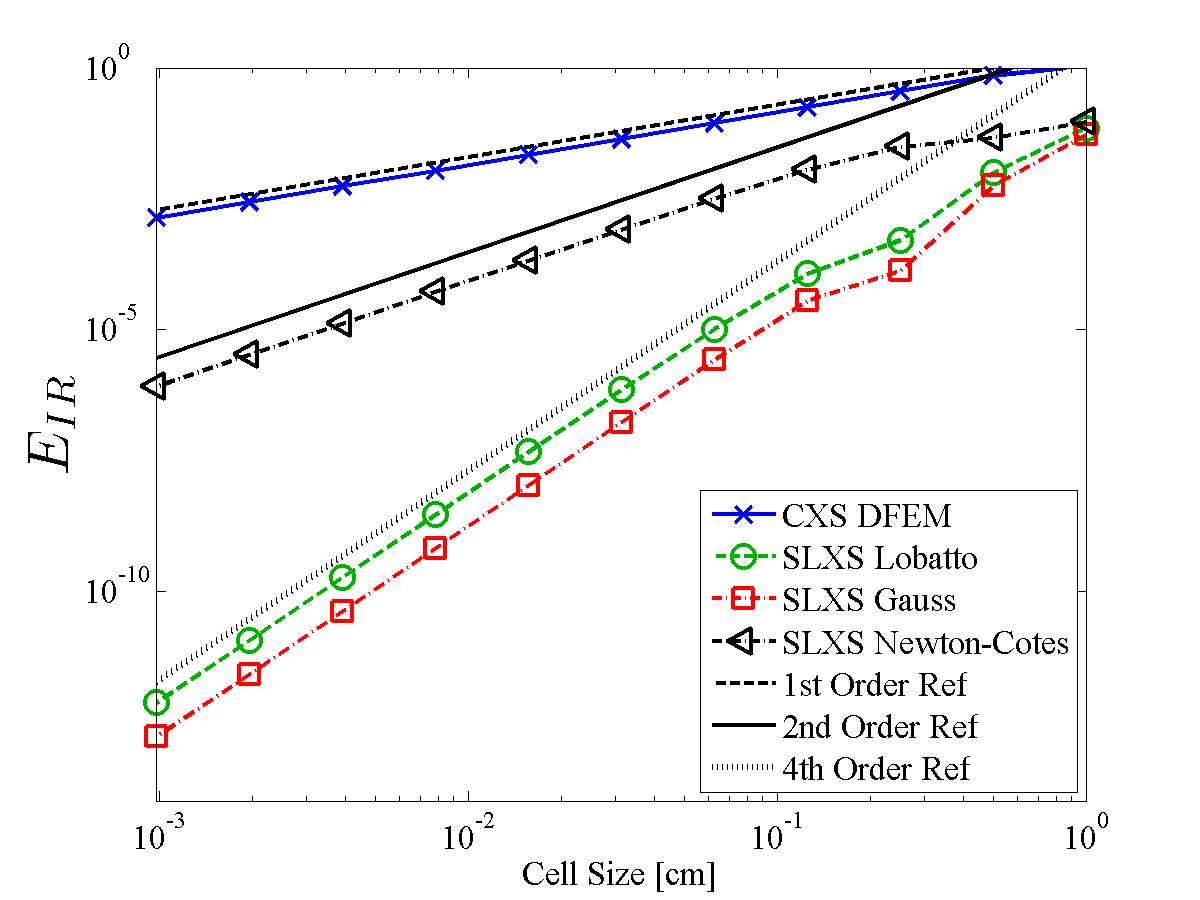
\includegraphics[width=10cm]{chapter3_variable_xs/P3_VarXS_E_I_L2.png}
\caption{Convergence of $E_{IR}$  for a pure absorber with exponentially varying cross section discretized with cubic DFEM.}
\label{fig:varxs_I_L2_p3}
\end{figure}
%
%
\begin{figure}[!htp]
\centering
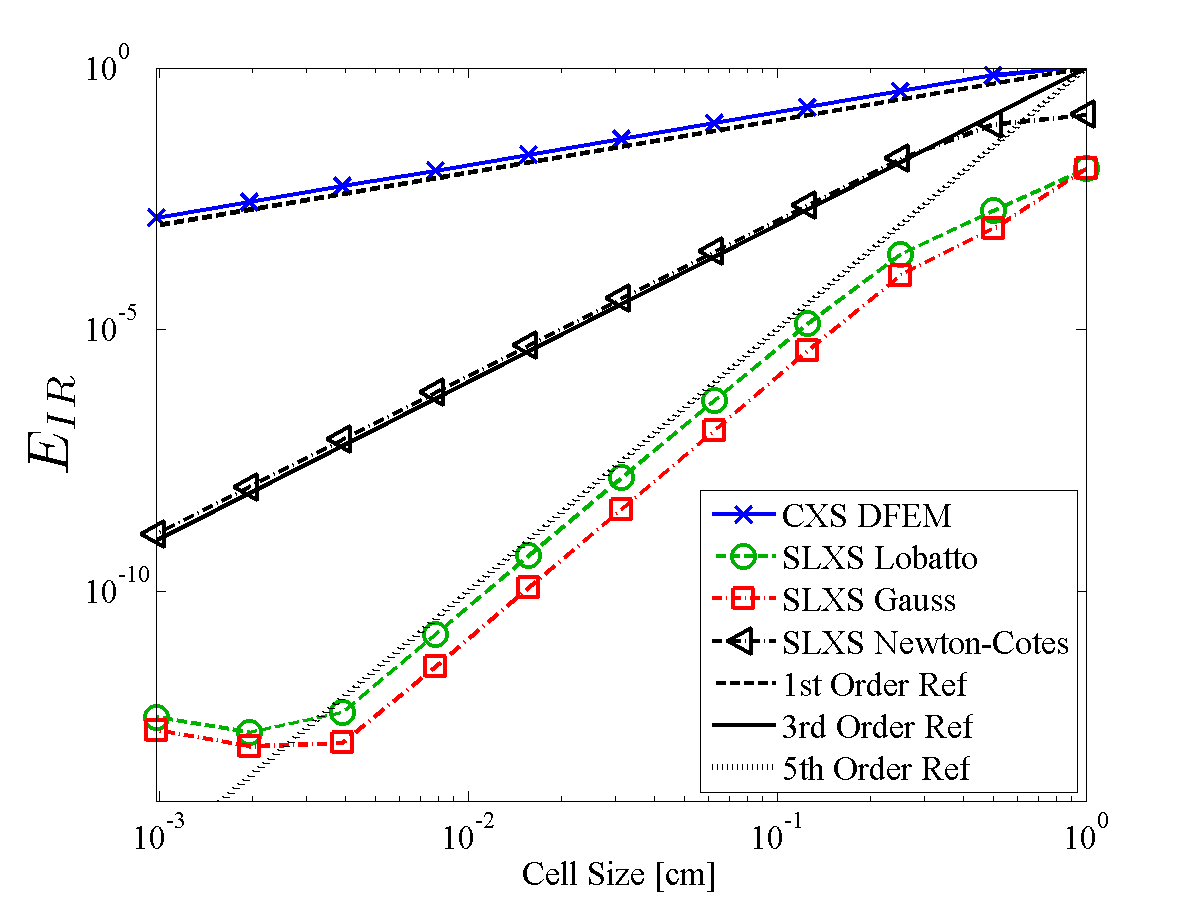
\includegraphics[width=10cm]{chapter3_variable_xs/P4_VarXS_E_I_L2.png}
\caption{Convergence of $E_{IR}$  for a pure absorber with exponentially varying cross section discretized with quartic DFEM.}
\label{fig:varxs_I_L2_p4}
\end{figure}
%%
%%
We observe the detrimental effect of approximating a spatially varying cross section with a constant in each spatial cell when we examine the $L_2$ convergence results for the interaction rate, $E_{IR}$, for the CXS DFEM scheme.
Regardless of angular flux trial space polynomial degree, CXS DFEM converges $E_{IR}$ to only first order in space.
However, the self-lumping schemes exhibit the same trends in converging $E_{IR}$ (in the $L^2$-norm sense) as exhibited in converging $E_{\psi}$:
\begin{itemize}
\item SLXS Lobatto and SLXS Gauss converge $E_{IR}$ with order $P+1$,
\item SLXS Gauss is more accurate than SLXS Lobatto by a constant, and
\item SLXS Newton-Cotes converges $E_{IR}$ second order in space for odd degree trial spaces and third order in space for even degree trial spaces.
\end{itemize}  

Convergence data for $E_{IR_A}$ as function of cell size for linear - quartic trial spaces is given in \figs{fig:varxs_I_A_p1}{fig:varxs_I_A_p4}.
%
%%%
\begin{figure}[!htp]
\centering
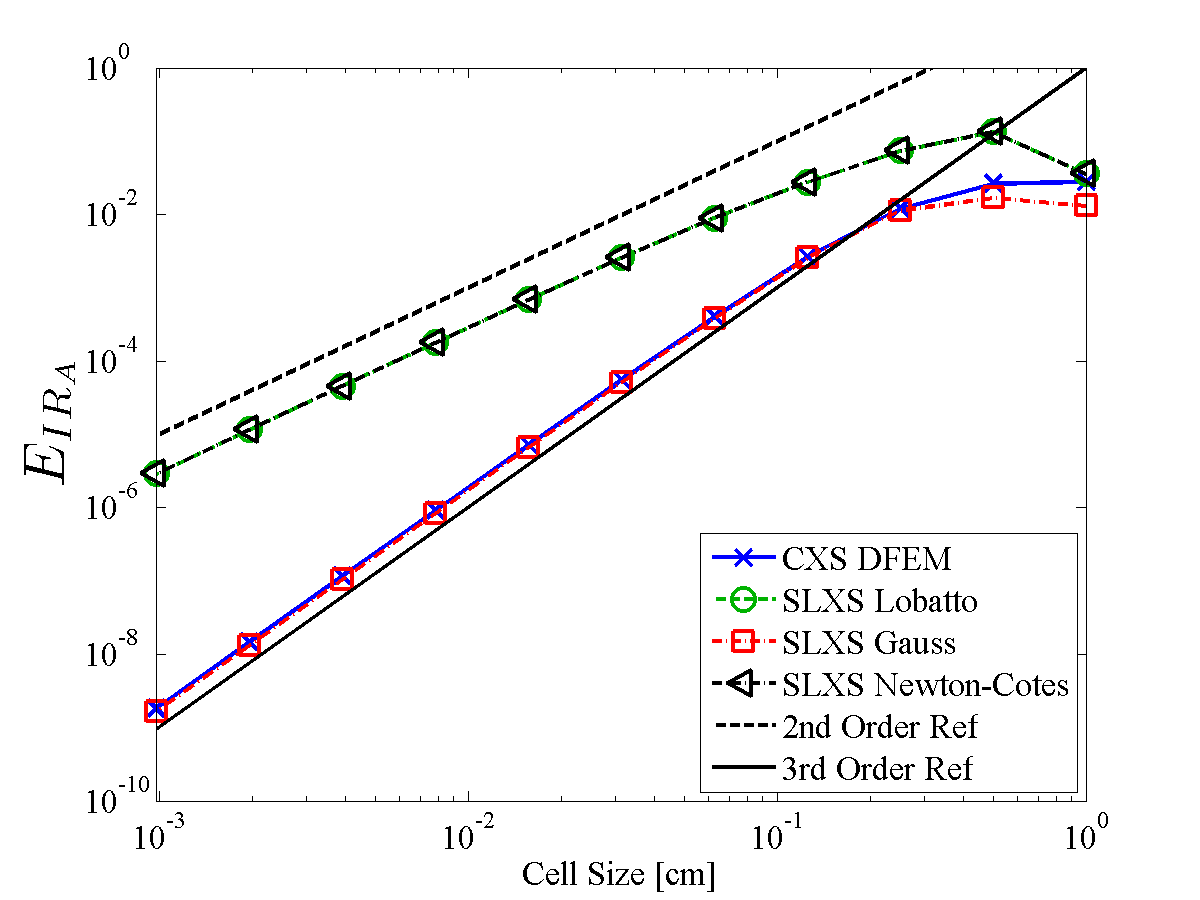
\includegraphics[width=10cm]{chapter3_variable_xs/P1_VarXS_E_I_A.png}
\caption{Convergence of $E_{IR_A}$ for a pure absorber with exponentially varying cross section discretized with linear DFEM.}
\label{fig:varxs_I_A_p1}
\end{figure}
%
%
\begin{figure}[!hbp]
\centering
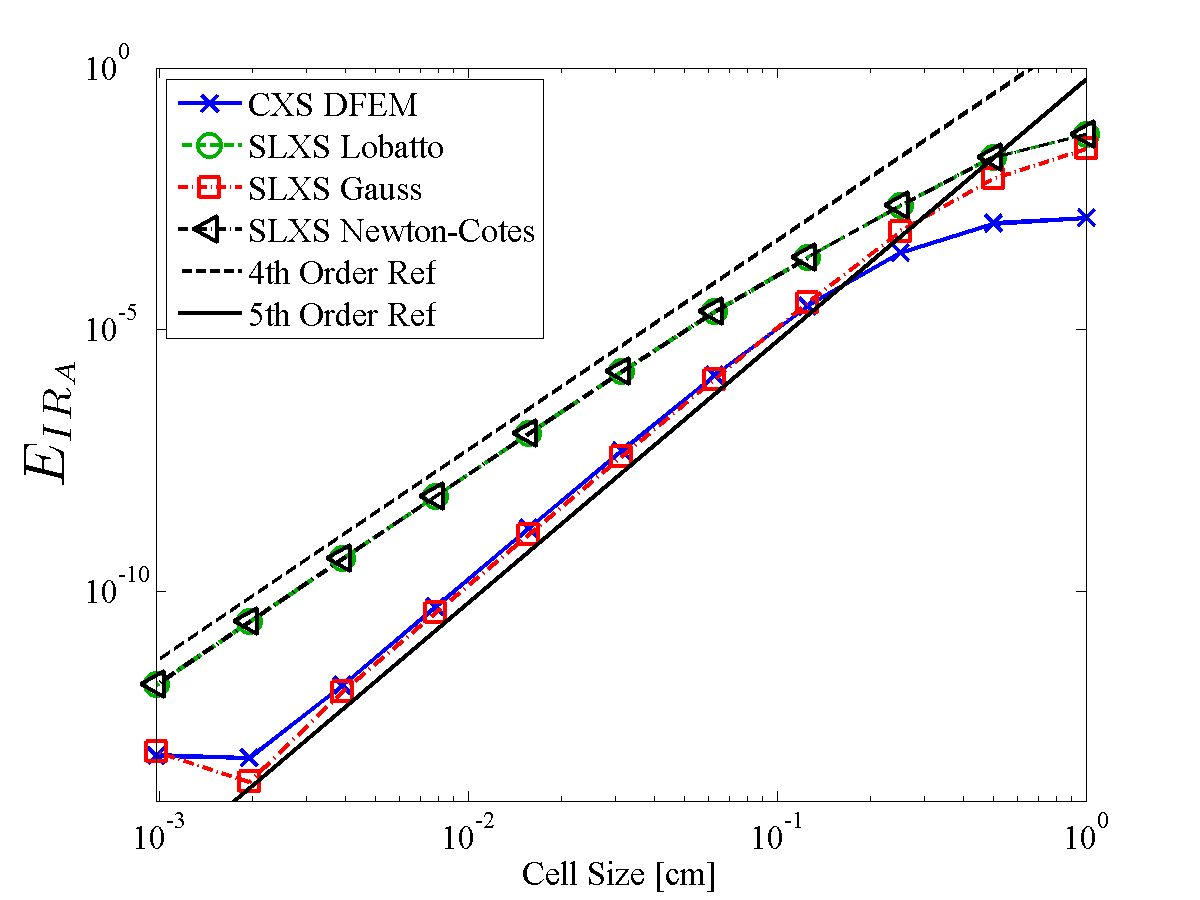
\includegraphics[width=10cm]{chapter3_variable_xs/P2_VarXS_E_I_A.png}
\caption{Convergence of $E_{IR_A}$ for a pure absorber with exponentially varying cross section discretized with quadratic DFEM.}
\label{fig:varxs_I_A_p2}
\end{figure}
%
%%
\begin{figure}[!htp]
\centering
\includegraphics[width=10cm]{chapter3_variable_xs/P3_VarXS_E_I_A.png}
\caption{Convergence of $E_{IR_A}$ for a pure absorber with exponentially varying cross section discretized with cubic DFEM.}
\label{fig:varxs_I_A_p3}
\end{figure}
\begin{figure}[!hbp]
\centering
\includegraphics[width=10cm]{chapter3_variable_xs/P4_VarXS_E_I_A.png}
\caption{Convergence of $E_{IR_A}$ for a pure absorber with exponentially varying cross section discretized with quartic DFEM.}
\label{fig:varxs_I_A_p4}
\end{figure}
The convergence results for the error in cell average interaction rate, $E_{IR_A}$, shown in \figs{fig:varxs_I_A_p1}{fig:varxs_I_A_p4}, do not behave as intuitively as the convergence rates for $E_{IR}$ observed in \figs{fig:varxs_I_L2_p1}{fig:varxs_I_L2_p4}.  
Given the poor performance of CXS DFEM in converging $E_{IR}$, one would expect that CXS DFEM would converge $E_{IR_A}$ poorly as well.  
However, this is not the case and CXS DFEM converges $E_{IR_A}$ with the same order of convergence as the best performing self-lumping scheme considered.

CXS DFEM converges $E_{IR_A}$ with a high-order of accuracy because of the locally conservative properties of DFEM approximations, that is:
\benum
\text{Particles Into Cell} - \text{Particles Out of Cell} =  \text{Total Interactions in Cell} \pep
\label{eq:chap3_balance}
\eenum
As shown in \figs{fig:varxs_psi_out_p1}{fig:varxs_psi_out_p4}, CXS DFEM converges the quantities on the left hand side of \eqt{eq:chap3_balance} with the same order of accuracy as any self-lumping scheme considered; CXS DFEM is at least as accurate in calculating the particles into a cell (outflow from the previous cell) and out of the cell (outflow from the current cell) as any other scheme considered.
Since \eqt{eq:chap3_balance} holds regardless of the numerical scheme considered, it follows that CXS DFEM converges $E_{IR_A}$, the term in the right hand side of \eqt{eq:chap3_balance} summed over all cells, with the maximum order of convergence displayed by any of the DFEM schemes we consider here.
Figures \ref{fig:varxs_I_A_p1}-\ref{fig:varxs_I_A_p4} validate this conclusion.
CXS DFEM and SLXS Gauss exhibit the highest order of spatial convergence, converging $E_{IR_A}$ with order $\propto 2P + 1$.  
SLXS Newton-Cotes and SLXS Lobatto converge $E_{IR_A}$ with the same orders of convergence each method exhibits in converging $E_{\psi_A}$.
For this problem SLXS Lobatto converges $E_{IR_A} \propto 2P$ and SLXS Newton-Cotes converged $E_{IR_A} \propto P$.

%%%%%%%%%%%%%%%%%%%%%%%%%%%%%%%%%%%%%%%%%%%%%%%%%%%%%%%%%%%%%%%%%%%%%
\subsection{Consequences of Assuming a Cell-Wise Constant Cross Section}
%%%%%%%%%%%%%%%%%%%%%%%%%%%%%%%%%%%%%%%%%%%%%%%%%%%%%%%%%%%%%%%%%%%%%

To more fully understand the poor convergence of point-wise error in angular flux and interaction rate, $E_{\psi}$ and $E_{IR}$, associated with CXS DFEM  we now examine more closely the CXS DFEM spatial approximations to $\psi(x,\mu_d)$ and $IR(x)$. 
We again consider a pure absorber with total absorption cross section that varies exponentially in space with $c_1 = 0.1$, and $c_2 = 2\ln(10)$.  
A beam of radiation is incident on the left face in the direction of $\mu_d=1$, vacuum boundary conditions are applied on the right face of the slab, and $x\in[0, 1]$.    

In \fig{fig:cxs_blades_psi}, we plot the exact $\psi(x)$ and in \fig{fig:cxs_blades_ir}, we plot $IR(x)$.  
Additionally we plot the respective CXS DFEM numerical approximations, $\widetilde{\psi}(x)$ and $\widetilde{IR}(x)$, using $N_{cells}=5$, and $\hat{\Sigma}_{t,i}$ as defined in \eqt{eq:chap3_cxs_sigma}. 
Also plotted in \fig{fig:cxs_blades_psi} and \fig{fig:cxs_blades_ir}, we plot the analytic angular flux and reaction rate, respectively, one would obtain if the cell average cross section, $\hat{\Sigma}_{t,i}$, had been used instead of the true $\Sigma_t(x)$.
We refer to these analytic solutions as $\psi_C(x)$ and $IR_C(x)$.
\begin{figure}[!hbp]
\centering
\includegraphics[width=12cm]{chapter3_variable_xs/Psi_Blades.png}
\caption{Plots of the analytic $\psi(x)$, CXS DFEM $\widetilde{\psi}(x)$, and $\psi_C(x)$ for the pure absorber with exponential cross section.}
\label{fig:cxs_blades_psi}
\end{figure}

\begin{figure}[!htp]
\centering
\includegraphics[width=12cm]{chapter3_variable_xs/I_Blades.png}
\caption{Plots of the analytic $IR(x)$, CXS DFEM $\widetilde{IR}(x)$, and  $IR_C(x)$ for the pure absorber with exponential cross section.}
\label{fig:cxs_blades_ir}
\end{figure}
%%%
%%%if instead of being the exponentially varying $\Sigma_t(x)$, total macroscopic cross section, was a piecewise constant function, $\Sigma_{t,C}(x)$, equal to $\hat{\Sigma}_{t,i}$, such that:
%%%\benum
%%%\Sigma_{t,C}(x) = \frac{1}{\Delta x_i}\int_{x_{i-1/2}}^{x_{i+1/2}}{\Sigma_1 A^{\Sigma_2 x}~dx},~~x\in[x_{i-1/2},x_{i+1/2}] \pec
%%%\eenum
%%%where $x_{i\pm1/2}$ are the boundaries of cell $i$ used in by the CXS DFEM scheme.
%%%We refer to the analytic angular flux and interaction rate solutions of the problem where total macroscopic cross section is $\Sigma_{t,C}(x)$ as $\psi_C(x)$ and $I_C(x)$, respectively.

Since CXS DFEM is a discontinuous scheme, some discontinuity is expected in the plot of $\widetilde{\psi}$ in \fig{fig:cxs_blades_psi} and of $\widetilde{IR}$ in \fig{fig:cxs_blades_ir}. 
However, the discontinuities present in \fig{fig:cxs_blades_ir} are highly disconcerting.
The analytic $IR(x)$ is smooth and does not vary rapidly within individual mesh cells, yet there are significant, non-monotonic discontinuities in the CXS DFEM interaction rate solution to the pure absorber problem with exponentially varying cross section.
The noticeably poor behavior of $\widetilde{IR}(x)$ in \fig{fig:cxs_blades_ir} is inherent to the assumption of a cell-wise constant cross section.
This inherent error of approximating a continuously varying cross section with cell-wise constants is clearly visible when comparing the plots of $IR_C(x)$ to $IR(x)$ in \fig{fig:cxs_blades_ir}.
The only difference and source of error in $IR_C(x)$ is the assumption of a cell-wise constant cross section.
%The only difference between these two sets of results is the approximation of $\Sigma_t(x) \approx \hat{\Sigma}_{t,i}$.
Figure \ref{fig:cxs_blades_psi} and \fig{fig:cxs_blades_ir} does not suggest that linear DFEM is unsuitable for use in problems with spatially varying cross sections. 
Rather, comparing the CXS DFEM $\widetilde{\psi}(x)$to $\psi_C(x)$ in \fig{fig:cxs_blades_psi} and $\widetilde{IR}(x)$ to $IR_C(x)$ in \fig{fig:cxs_blades_ir}, we see that CXS DFEM  is very accurate when compared to the analytic solution of the problem CXS DFEM is solving, a pure absorber with cell-wise constant cross section.
%
Given the poor accuracy of CXS DFEM in approximating the true $\psi(x)$ and $IR(x)$, we wish to see how a scheme that does not assume a cell-wise constant cross section behaves.
Consider $\widetilde{\psi}(x)$ and $\widetilde{IR}(x)$ obtained with SLXS Lobatto using a linear DFEM trial space and five spatial cells, shown in \fig{fig:lobatto_blades_psi} amd \fig{fig:lobatto_blades_ir}, for the same problem.  
In \fig{fig:lobatto_blades_psi}, the differences between the angular flux solutions obtained using (1) a cell-wise constant cross section (CXS DFEM) and (2) evaluating cross section values at quadrature points (SLXS Lobatto) are small.
\begin{figure}[!htp]
\centering
\includegraphics[width=12cm]{chapter3_variable_xs/SLXS_Psi_Profile.png}
\caption{Plot of the linear trial space SLXS Lobatto and CXS DFEM approximations of $\widetilde{\psi}(x)$ for the pure absorber problem with exponentially varying cross section.}
\label{fig:lobatto_blades_psi}
\end{figure}
%
\\
This is not the case when comparing the different approximations to the interaction rate, $\widetilde{IR}(x)$, in \fig{fig:lobatto_blades_ir}.  
Though there are discontinuities in the SLXS Lobatto $\widetilde{IR}(x)$, the discontinuities are smaller and the SLXS Lobatto $\widetilde{IR}(x)$ is monotonic unlike the CXS DFEM $\widetilde{IR}(x)$.   
The SLXS Lobatto $\widetilde{IR}(x)$ is clearly more accurate than the CXS DFEM $\widetilde{IR}(x)$.
%
\begin{figure}[!htp]
\centering
\includegraphics[width=12cm]{chapter3_variable_xs/SLXS_I_Profile.png}
\caption{Plot of the linear trial space SLXS Lobatto and CXS DFEM approximations of $\widetilde{IR}(x)$ for the pure absorber problem with exponentially varying cross section.}
\label{fig:lobatto_blades_ir}
\end{figure}
%
%
\\
In this problem, there are two possible sources of error that could cause a DFEM to be inaccurate: inexact matrix evaluation and not incorporating cross-section spatial variation into the scheme.
By definition, CXS DFEM exactly integrates the mass matrix, and we showed in \secref{sec:chapter2_constant_xs} that schemes that exactly integrate the mass matrix are more accurate than schemes that only approximately integrate the mass matrix, like SLXS Lobatto.
Thus, the poor accuracy of CXS DFEM relative to SLXS Lobatto is entirely caused by the approximation of a spatially varying cross section with a cell-wise constant value.

The ``blading'' in $\widetilde{IR}(x)$ has not previously been reported in neutron transport or thermal radiative transport community literature.
We are likely not the first to have generated these large, non-monotonic discontinuities. 
In fact, we believe that blading has frequently been present in DFEM both neutron transport and thermal radiatve transfer simulations but has likely gone unnoticed due to the prevalence of linear DFEM and simplified data visualization using cell midpoint values.

To demonstrate that a minor choice in data presentation can obscure the existence of blading, consider \fig{fig:cxs_avg_psi} and \fig{fig:cxs_avg_ir} that linearly interpolate between $\widetilde{\psi}_{A,i}$ and  $\widetilde{IR}_{A,i}$ plotted at cell centers.
Though \fig{fig:cxs_avg_psi} is visually indistinguishable from \fig{fig:cxs_blades_psi}, the blading of $\widetilde{IR}(x)$ present in \fig{fig:cxs_blades_ir} is not at all visually present in \fig{fig:cxs_avg_ir}.
Interaction rate terms are present in other radiation transport physics.
In particular, we think of the radiative transfer analog to the neutronics interaction rate, absorption rate density.
We hypothesize here, and will show in \secref{sec:chapter6_grey_radtran} that assuming cell-wise constants opacities for problems with temperature dependent opacities introduces blading in thermal radiative transfer temperature solutions, via the material energy equation's absorption rate density term.
\vfill{}

\begin{figure}[!htp]
\centering
\includegraphics[width=11cm]{chapter3_variable_xs/CXS_Psi_A_Profile.png}
\caption{Plot of the CXS DFEM cell average angular flux at cell centers with linear interpolation for a pure absorber with exponentially varying spatial cross section.}
\label{fig:cxs_avg_psi}
\end{figure}
%
\begin{figure}[!hbp]
\centering
\includegraphics[width=11cm]{chapter3_variable_xs/CXS_I_A_Profile.png}
\caption{Plot of the CXS DFEM cell average interaction rate at cell centers with linear interpolation for a pure absorber with exponentially varying spatial cross section.}
\label{fig:cxs_avg_ir}
\end{figure}


%%%%%%%%%%%%%%%%%%%%%%%%%%%%%%%%%
%
\subsection{Flux-Weighting versus Volume-Averaged Cross Sections}

In our results thus far, we have only considered volume-averaged cell-wise cross sections(the CXS DFEM scheme).
However, in reactor physics problems, a flux-weighted cross section is often used to generate spatially averaged cross sections \cite{bell_glasstone}.
We now introduce the flux-weighted cell-wise constant cross section scheme (FW CXS), which differs from the CXS DFEM scheme only by how $\hat{\Sigma}$ is defined in each cell.  
For the FW CXS scheme, we define $\hat{\Sigma}_i$ as
\benum
\hat{\Sigma}_i = \frac{\int_{x_{i-1/2}}^{x_{i+1/2}}{ \Sigma(x) \psi(x,\mu_d)~dx}}{\int_{x_{i-1/2}}^{x_{i+1/2}}{ \psi(x,\mu_d)~dx}} \pep
\label{eq:chap3_fw_cxs}
\eenum
In practice, flux-weighting is often done using the scalar flux in order not to have angle-dependent total cross section.  
However for the beam problem we consider here, $\psi(x,\mu_d)$ is proportional to the scalar flux.

We first compare the accuracy of FW CXS versus  volume-averaged CXS DFEM for a cubic DFEM trial space, as shown in \figs{fig:fw_accuracy_psi}{fig:fw_accuracy_ir_a}.  
In \figs{fig:fw_accuracy_psi}{fig:fw_accuracy_ir_a}, we omit a plot of $E_{\psi_{out}}$ as we have already demonstrated that the accuracy of any method in calculating $E_{\psi_{out}}$ determines the method's accuracy in calculating $E_{IR_A}$.  
That is, if $E_{IR_A}$ converges at a given rate, $E_{\psi_{out}}$ converges at the same rate.  

Figures \ref{fig:fw_accuracy_psi}-\ref{fig:fw_accuracy_ir} show that FW CXS scheme is more accurate than CXS DFEM when comparing $E_{\psi}$, $E_{\psi_A}$ and, at low resolutions, $E_{IR}$.
However, though designed to preserve cell average interaction rates, FW CXS scheme is not only less accurate than  CXS DFEM in calculating cell average interaction rates, it converges $E_{IR_A}$ at most second order in space, whereas a volume-averaged cross section converges $E_{IR_A}$ $\propto 2P+1$ for the pure absorber problem.
\vfill{}
%
%
\begin{figure}[!htp]
\centering
\includegraphics[width=11cm]{chapter3_variable_xs/FW_XS_P3_VarXS_E_psi_L2.png}
\caption{Accuracy comparison of flux weighted constant cross section scheme (FW CXS) to volume averaged cross section  scheme (CXS DFEM) with a cubic angular flux trial space.}
\label{fig:fw_accuracy_psi}
\end{figure}
%
%
\begin{figure}[!hbp]
\centering
\includegraphics[width=11cm]{chapter3_variable_xs/FW_XS_P3_VarXS_E_psi_A.png}
\caption{Accuracy comparison of flux weighted constant cross section scheme (FW CXS) to volume averaged cross section  scheme (CXS DFEM) with a cubic angular flux trial space.}
\label{fig:fw_accuracy_psi_a}
\end{figure}
%
%
\begin{figure}[!htp]
\centering
\includegraphics[width=11cm]{chapter3_variable_xs/FW_XS_P3_VarXS_E_I_L2.png}
\caption{Accuracy comparison of flux weighted constant cross section scheme (FW CXS) to volume averaged cross section  scheme (CXS DFEM) with a cubic angular flux trial space.}
\label{fig:fw_accuracy_ir}
\end{figure}
%
%
\begin{figure}[!hbp]
\centering
\includegraphics[width=11cm]{chapter3_variable_xs/FW_XS_P3_VarXS_E_I_A.png}
\caption{Accuracy comparison of flux weighted constant cross section scheme (FW CXS) to volume averaged cross section  scheme (CXS DFEM) with a cubic angular flux trial space.}
\label{fig:fw_accuracy_ir_a}
\end{figure}

Finally, we consider the FW CXS scheme's $\widetilde{\psi}(x)$ in \fig{fig:fw_blading_psi} and $\widetilde{IR}(x)$ in \fig{fig:fw_blading_ir}.  
In \fig{fig:fw_blading_psi} and \fig{fig:fw_blading_ir} the FW CXS and CXS DFEM schemes calculate slightly different solution representations.
However, the FW CXS scheme  exhibits the same interaction rate blading phenomena as the CXS DFEM scheme, reiterating that blading is a result of approximating a spatially varying cross section as a cell-wise constant.
The choice of cell-wise cross section does not eliminate blading.
\begin{figure}[!hbp]
\centering
\includegraphics[width=12cm]{chapter3_variable_xs/FW_Psi_Blades.png}
\caption{Plot of the linear trial space FW CXS and CXS DFEM approximations to $\widetilde{\psi}(x)$ for the pure absorber problem with exponentially varying spatial cross section.}
\label{fig:fw_blading_psi}
\end{figure}
%
%
\begin{figure}[!htp]
\centering
\includegraphics[width=12cm]{chapter3_variable_xs/FW_I_Blades.png}
\caption{Plot of the linear trial space FW CXS and CXS DFEM approximations to $\widetilde{IR}(x)$ for the pure absorber problem with exponentially varying spatial cross section.}
\label{fig:fw_blading_ir}
\end{figure}
%
%%%%%%%%%%%%%%%%%%%%%%%%%%%%%%%%%
%
%%%%%%%%%%%%%%%%%%%%%%%%%%%%%%%%%
%
%\subsection{Effects of Mesh Spacing}
%%%%%%%%%%%%%%%%%%%%%%%%%%%%%%%%%
%
In practice, computational domains are not necessarily discretized with uniform grids; rather cells are concentrated in regions where the solution is known or assumed to vary rapidly.  
For the pure absorber problem, we compare two alternative methods of mesh spacing (logarithmic grids and equal optical thickness grids, see \tbl{tbl:spacing_labels}),
to the results obtained with equally-spaced mesh cells.
\begin{table}
\centering
\caption{Shorthand notation of different cell spacing schemes.}
\begin{tabular}{|c|c|}
\hline
Spacing Label & Spacing Type \\
\hline
EQUAL & Equally-spaced cells \\
\hline
MFP & Constant optical thickness cells \\
\hline
LOG & Logarithmically spaced cells \\
\hline
\end{tabular}
\label{tbl:spacing_labels}
\end{table}

We derive how to generate these meshes in \secref{sec:mesh_gen} and give results in \secref{sec:mesh_results}

\subsubsection{Generating Improved Spatial Meshes}  
\label{sec:mesh_gen}

Two alternative meshing strategies are compared to equally-spaced meshed.
In the following, we will use a shorthand notation, given in \tbl{tbl:spacing_labels}.
With the MFP meshing strategy, we find each cell width by determining the width of each cell from $i=1$ (leftmost cell) to $i=N_{cell}$ as outlined by \eqt{eq:chap3_mfp_spacing}:
\begin{subequations}
First, we determine the average cell optical thickness:
\label{eq:chap3_mfp_spacing}
\benum
\bar{h} = \frac{  \int_{x_{1/2}}^{x_{N_{cell}+1/2}}{ \Sigma_t(x)~dx} }{ N_{cell} } \pep
\eenum
Then, we solve the following equation for $x_{i+1/2}$:
\benum
\int_{x_{i-1/2}}^{x_{i+1/2}}{\Sigma_t(x)~dx} - \bar{h}  = 0 \pec
\eenum
yielding
\benum
x_{i+1/2} = \frac{1}{c_2} \log\left[ \frac{c_2( \bar{h} + \Sigma_t(x_{i-1/2}) }{c_1} \right] \pep
\eenum
\end{subequations}

There are several ways to specify LOG spacing, but we elected to set a ratio, $0.6$, between adjacent cell sizes with the caveat that we would set a minimum cell size, $\Delta x_{min}$.
In our convergence testing, at the first refinement when $\Delta x_{N_cell} < \Delta x_{min}$, the grid is ``fixed'' and all further refinements uniformly refine the ''fixed'' grid.  $\Delta x_{N_{cell}}$ is the cell width for the right most cell where, for $R < 1$,
\benum
\Delta x_i =\Delta x_1 R^{i-1}, ~i\in[1,N_{cell}] \pep
\eenum
$\Delta x_1$ is determined by requiring that the geometric series of cell widths completely fill the space:
\benum
\Delta x_1 = \left( x_{N_{cell}+1/2} - x_{1/2} \right) \frac{1-R}{1-R^{N_{cell} }}
\eenum
The grid is ``fixed'' by resetting the width of every cell whose width, if set to the value required for a purely logarithmically spaced grid with $R$ would be below  $\Delta x_{min}$, to $\Delta x_{min}$. 
After imposing this, cell widths are determined by requiring the cells that were not reset to fill the problem space logarithmically using $R$.
If there is no minimum cell width, at high mesh refinements, most cells will be infinitesimally small and the large cells will never be refined, causing error to stagnate. 
Logarithmic spacing represents the ``smart'' meshing strategy most likely to be employed in engineering practice as it requires the least amount of solution information prior to problem execution.  
For all of our calculations, we set $R=0.6$ and $\Delta x_{min} = 10^{-3}~[cm]$.

\subsubsection{Mesh Spacing Results}
\label{sec:mesh_results}

We begin our discussion of alternate mesh spacing by first noting that the choice of mesh spacing method does not alter asymptotic convergence rates, as shown in
\figs{fig:lobatto_spacing_psi}{fig:lobatto_spacing_ir_A}.  
The convergence of the SLXS Lobatto scheme using a quadratic trial space for 
$E_{\psi}$ is shown in \fig{fig:lobatto_spacing_psi}, 
for $E_{\psi_A}$ in \fig{fig:lobatto_spacing_psi_A}, for $E_{IR}$ in \fig{fig:lobatto_spacing_ir}, and for $E_{IR_A}$ 
in \fig{fig:lobatto_spacing_ir_A}.
Regardless of the choice of mesh spacing, all error quantities of interest converge at the same asymptotic rate. 
Plots showing other trial space degrees and DFEM schemes are omitted for brevity.  
We also omit showing the convergence of $E_{\psi_{out}}$ as we have already demonstrated that the convergence rate of $E_{\psi_{out}}$ and $E_{IR_A}$are related and identical.
\begin{figure}[!htp]
\centering
\includegraphics[width=11cm]{chapter3_variable_xs/P2_LOBATTO_E_PSI.png}
\caption{Asymptotic convergence of the SLXS Lobatto scheme using a quadratic trial space, for different mesh spacing methodologies.}
\label{fig:lobatto_spacing_psi}
\end{figure}
%
%
\begin{figure}[!hbp]
\centering
\includegraphics[width=11cm]{chapter3_variable_xs/P2_LOBATTO_E_PSI_A.png}
\caption{Asymptotic convergence of the SLXS Lobatto scheme using a quadratic trial space, for different mesh spacing methodologies.}
\label{fig:lobatto_spacing_psi_A}
\end{figure}
%
%
\begin{figure}[!htp]
\centering
\includegraphics[width=11cm]{chapter3_variable_xs/P2_LOBATTO_E_IR.png}
\caption{Asymptotic convergence of the SLXS Lobatto scheme using a quadratic trial space, for different mesh spacing methodologies.}
\label{fig:lobatto_spacing_ir}
\end{figure}
%
%
\begin{figure}[!hbp]
\centering
\includegraphics[width=11cm]{chapter3_variable_xs/P2_LOBATTO_E_IR_A.png}
\caption{Asymptotic convergence of the SLXS Lobatto scheme using a quadratic trial space, for different mesh spacing methodologies.}
\label{fig:lobatto_spacing_ir_A}
\end{figure}
%
%

At mesh refinements that are not in the asymptotic convergence regime, the intelligent meshing can result in a significant reduction in error.  
Consider the difference smart meshing has in reducing $E_{\psi}$, $E_{\psi_A}$, $E_{IR}$, and $E_{IR_A}$ for the SLXS Lobatto scheme in
\figs{fig:low_res_lobatto_psi}{fig:low_res_lobatto_ir_A}, for the SLXS Gauss scheme in \figs{fig:low_res_gauss_psi}{fig:low_res_gauss_ir_A}, 
and for CXS DFEM in \figs{fig:low_res_cxs_psi}{fig:low_res_cxs_ir_A} when using a quadratic DFEM trial space at low cell resolutions.
\begin{figure}[!hbp]
\centering
\includegraphics[width=11cm]{chapter3_variable_xs/LOW_RES_P2_LOBATTO_E_PSI.png}
\caption{Errors associated with the SLXS Lobatto using a quadratic trial space scheme for different mesh spacing methodologies, at low resolutions.}
\label{fig:low_res_lobatto_psi}
\end{figure}
\vfill{}
\pagebreak

%
\begin{figure}[!htp]
\centering
\includegraphics[width=11cm]{chapter3_variable_xs/LOW_RES_P2_LOBATTO_E_PSI_A.png}
\caption{Errors associated with the SLXS Lobatto using a quadratic trial space scheme for different mesh spacing methodologies, at low resolutions.}
\label{fig:low_res_lobatto_psi_A}
\end{figure}
%
%
\begin{figure}[!hbp]
\centering
\includegraphics[width=11cm]{chapter3_variable_xs/LOW_RES_P2_LOBATTO_E_IR.png}
\caption{Errors associated with the SLXS Lobatto using a quadratic trial space scheme for different mesh spacing methodologies, at low resolutions.}
\label{fig:low_res_lobatto_ir}
\end{figure}

\pagebreak
%
\begin{figure}[!htp]
\centering
\includegraphics[width=11cm]{chapter3_variable_xs/LOW_RES_P2_LOBATTO_E_IR_A.png}
\caption{Errors associated with the SLXS Lobatto using a quadratic trial space scheme for different mesh spacing methodologies, at low resolutions.}
\label{fig:low_res_lobatto_ir_A}
\end{figure}
%%
%%
\begin{figure}[!hbp]
\centering
\includegraphics[width=11cm]{chapter3_variable_xs/LOW_RES_P2_GAUSS_E_PSI.png}
\caption{Errors associated with the SLXS Gauss using a quadratic trial space for different mesh spacing methodologies, at low resolutions.}
\label{fig:low_res_gauss_psi}
\end{figure}
%
\begin{figure}[!htp]
\centering
\includegraphics[width=11cm]{chapter3_variable_xs/LOW_RES_P2_GAUSS_E_PSI_A.png}
\caption{Errors associated with the SLXS Gauss using a quadratic trial space for different mesh spacing methodologies, at low resolutions.}
\label{fig:low_res_gauss_psi_A}
\end{figure}
%
\begin{figure}[!hbp]
\centering
\includegraphics[width=11cm]{chapter3_variable_xs/LOW_RES_P2_GAUSS_E_IR.png}
\caption{Errors associated with the SLXS Gauss using a quadratic trial space for different mesh spacing methodologies, at low resolutions.}
\label{fig:low_res_gauss_ir}
\end{figure}
%
\begin{figure}[!htp]
\centering
\includegraphics[width=11cm]{chapter3_variable_xs/LOW_RES_P2_GAUSS_E_IR_A.png}
\caption{Errors associated with the SLXS Gauss using a quadratic trial space for different mesh spacing methodologies, at low resolutions.}
\label{fig:low_res_gauss_ir_A}
\end{figure}
%
%
\begin{figure}[!hbp]
\centering
\includegraphics[width=11cm]{chapter3_variable_xs/LOW_RES_P2_CXS_E_PSI.png}
\caption{Errors associated with CXS DFEM using a quadratic trial space  for different mesh spacing methodologies, at low resolutions.}
\label{fig:low_res_cxs_psi}
\end{figure}
%
\begin{figure}[!htp]
\centering
\includegraphics[width=11cm]{chapter3_variable_xs/LOW_RES_P2_CXS_E_PSI_A.png}
\caption{Errors associated with CXS DFEM using a quadratic trial space  for different mesh spacing methodologies, at low resolutions.}
\label{fig:low_res_cxs_psi_A}
\end{figure}
%
\begin{figure}[!hbp]
\centering
\includegraphics[width=11cm]{chapter3_variable_xs/LOW_RES_P2_CXS_E_IR.png}
\caption{Errors associated with CXS DFEM using a quadratic trial space  for different mesh spacing methodologies, at low resolutions.}
\label{fig:low_res_cxs_ir}
\end{figure}
%
\begin{figure}[!htp]
\centering
\includegraphics[width=11cm]{chapter3_variable_xs/LOW_RES_P2_CXS_E_IR_A.png}
\caption{Errors associated with CXS DFEM using a quadratic trial space  for different mesh spacing methodologies, at low resolutions.}
\label{fig:low_res_cxs_ir_A}
\end{figure}
First, we note that any particular mesh spacing methodology results in solutions that are more accurate for certain quantities, but not for all quantities.  
For example, with the self-lumping schemes, $E_{\psi}$ is generally smaller when using an equally spaced mesh, but using the LOG mesh results in orders of magnitude improvement in $E_{IR}$ and $E_{IR_A}$ on coarse meshes.
Figures \ref{fig:low_res_cxs_psi}-\ref{fig:low_res_cxs_ir_A}, CXS DFEM again illustrates that LOG spacing is more accurate in calculating interaction rate quantities than an equally-spaced mesh and equally-spaced meshes are generally more accurate than other meshing strategies for calculating angular flux quantities.
However, CXS DFEM shows a two order of magnitude reduction in calculating $E_{IR_A}$ when using a mesh that has a uniform optical thickness in each cell.  This is a direct result of CXS DFEM converging as $\hat{\sigma} \Delta x \to 0$.
\vfill{}

%
%

%\label{sec:chap3_mesh_results}
%The important results from Figs. \ref{fig:lobatto_spacing}-\ref{fig:low_res_cxs} are summarized here:
%\begin{enumerate}
%\item mesh spacing does not affect asymptotic order of convergence,
%\item accuracy in calculating certain quantities of interest (point-wise and cell averaged reaction rates) is improved with alternative meshing strategies at low resolution.
%%\item accuracy in calculating the angular flux, is sacrificed.
%\end{enumerate}

%%%%%%%%%%%%%%%%%%%%%%%%%%%%%%%%%%%%%%%%%%%%%%%%%%%
%
%  New template code for TAMU Theses and Dissertations starting Fall 2012.  
%  For more info about this template or the 
%  TAMU LaTeX User's Group, see http://www.howdy.me/.
%
%  Author: Wendy Lynn Turner 
%	 Version 1.0 
%  Last updated 8/5/2012
%
%%%%%%%%%%%%%%%%%%%%%%%%%%%%%%%%%%%%%%%%%%%%%%%%%%%
%%%%%%%%%%%%%%%%%%%%%%%%%%%%%%%%%%%%%%%%%%%%%%%%%%%%%%%%%%%%%%%%%%%%%%



\chapter{\uppercase{Iterative Acceleration for the $S_N$ Neutron Transport Equations}}
\label{sec:chapter4_acceleration}

Thus far, we have failed to discuss how the global system of angular flux unknowns is solved, 
focusing instead on the solution of a single system of equations that describes the unknowns of a single spatial cell, for a single discrete direction.
We have implicitly assumed the existence and knowledge of a transport sweep \cite{lewis_book}, or single, un-accelerated Richardson iteration.
In \secref{sec:dsa_basis}, we explain the fundamental iterative techniques used to solve the neutron transport equation for scatter media.
In \secref{sec:synthetics} we discuss the choices available for synthetic acclerators.
Finally  we two different synthetic acceleration techniques compatible with our chose spatial discretizations of the transport equation.
In \secref{sec:s2sa} we derive the $S_2$ synethetic acceleration (S2SA) technique\cite{s2sa} and in \secref{sec:dsa} we derive a modified interior penalty (MIP) diffusion synthetic accleration\cite{mip_dsa} (DSA) operator.  Finally, in \secref{sec:accel_results}, we compare verify the implementation of each for a set of test problems with spatially constant and and spatially varying interaction cross sections.


\section{Iterative Solution of the Neutron Transport $S_N$ Equations}
\label{sec:dsa_basis}

To describe the the iterative process by which the discrete ordinates neutron transport equations are solved, we re-visit the spatially analytic,
steady-state, mono-energetic discrete ordinates neutron transport equation, but do not have a monolithic right hand side source.
Rather, we treat the right hand side as having both an isotropic scattering component, and a fixed source component, as given in \eqt{eq:chap4_transport}.
\benum
\mu \frac{d \psi_d}{d x} + \Sigma_t \psi_d = \frac{\Sigma_s}{4\pi}\phi + S_d \pep
\label{eq:chap4_transport}
\eenum
The traditional practice is to solve \eqt{eq:chap4_transport} iteratively with Richardson iteration.  
Each Richardson iteration is referred to as a transport sweep, where for a fixed right hand side, $\psi_d$ is update direction by direction, cell be cell, sweeping 
from each direction's incident boundary through the entire mesh with upwinding at cell interfaces.
Introducing iteration index $\ell$, this process can be written as:
\benum
\mu \frac{d \psi_d^{(\ell+1)} }{d x} + \Sigma_t \psi_d^{(\ell+1)} = \frac{\Sigma_s}{4\pi}\phi^{(\ell)} + S_d \pep
\label{eq:chap4_iter}
\eenum
After we find, $\psi_d^{(\ell+1)}$, we update $\phi^{(\ell+1)}$ using the discrete ordinates definition:
\benum
\phi^{(\ell+1)} = 2\pi \sum_{d=1}^{N_{dir}}{w_d \psi_d^{(\ell+1)}} \pep
\eenum
Though convergent, the source iteration process can converge arbitrarily slow, as shown by Larsen\cite{larsen_dsa}, when $\frac{\Sigma_s}{\Sigma_t} \to 1$.
To accelerate the convergence of source iteration, the diffusion synthetic acceleration (DSA) technique was developed \cite{old_dsa}.
DSA is best explained through example.  

To start, we consider to a single source iteration:
\benum
\label{eq:chap4_iter1}
\mu \frac{d \psi_d^{(\ell+1/2)} }{d x} + \Sigma_t \psi_d^{(\ell+1/2)} = \frac{\Sigma_s}{4\pi}\phi^{(\ell)} + S_d \pep
\eenum
Subtracting \eqt{eq:chap4_transport} from \eqt{eq:chap4_iter1} yields:
\benum
\label{eq:chap4_err}
\mu \frac{d \delta \psi_d^{(\ell+1/2)} }{d x} + \Sigma_t \delta \psi_d^{(\ell+1/2)} = \frac{\Sigma_s}{4\pi} \delta \phi^{(\ell)} \pec
\eenum
where we have defined the iterative error of the angular flux, $\delta \psi_d^{(\ell+1)}$,
\benum
\psi_d = \psi_d^{(\ell+1)} + \delta \psi_d^{(\ell+1)} \pec
\eenum
and scalar flux iterative error, $\delta \phi^{(\ell)}$
\benum
\label{eq:chap4_phi_err}
\phi = \phi^{(\ell)} + \delta \phi_d^{(\ell)} \pep
\eenum
Subtracting $\frac{\Sigma_s}{4\pi} \delta \phi^{(\ell)}$ from both sides of \eqt{eq:chap4_err}, we see arrive at:
\benum
\mu \frac{d \delta \psi_d^{(\ell+1/2)} }{d x} + \Sigma_t \delta \psi_d^{(\ell+1/2)} - \frac{\Sigma_s}{4\pi} \delta \phi^{(\ell+1/2)}
= \frac{\Sigma_s}{4\pi} \delta \phi^{(\ell)} - \frac{\Sigma_s}{4\pi} \delta \phi^{(\ell+1/2)} \pep
\label{eq:chap4_intermediate}
\eenum
Recognizing:
\begin{subequations}
\beanum
\phi &=& \phi^{(\ell+1/2)} + \delta \phi^{(\ell+1/2)} \pec\\
\phi &=& \phi^{(\ell)} + \delta \phi^{(\ell)} \pec \\
\phi^{(\ell+1/2)} - \phi^{(\ell)} &=& \left( \phi - \delta \phi^{(\ell+1/2)}  \right) - \left( \phi -  \delta \phi^{(\ell)} \right) \pec \text{ and} \\
 \delta  \phi^{(\ell)} - \delta \phi^{(\ell+1)} &=& \phi^{(\ell+1/2)} - \phi^{(\ell)} \pec
\eeanum
\end{subequations}
\eqt{eq:chap4_intermediate} becomes:
\benum
\label{eq:dsa_idea}
\mu \frac{d \delta \psi_d^{(\ell+1/2)} }{d x} + \Sigma_t \delta \psi_d^{(\ell+1/2)} 
= \frac{\Sigma_s}{4\pi} \delta \phi^{(\ell+1/2)} + \frac{\Sigma_s}{4\pi} \left( \phi^{(\ell+1/2)} -  \phi^{(\ell)} \right) \pep
\eenum
Equation \ref{eq:dsa_idea} indicates that if we could solve a transport problem with a driving source equal to the difference between two scattering iterates,
\benum
\frac{\Sigma_s}{4\pi} \left( \phi^{(\ell+1/2)} - \phi^{(\ell)}  \right)\pec
\eenum
then we could get the iterative error of iteration $\delta \phi^{(\ell+1/2)}$, add to the $\phi^{(\ell+1/2)}$ we already have, and then have the exact solution, $\phi$. 
However, solving \eqt{eq:dsa_idea} is as difficult as solving the original problem in \eqt{eq:chap4_transport}.
Alternatively, if we could solve an approximation to \eqt{eq:dsa_idea}, perhaps the result would satisfy:
\benum
\label{eq:chap4_delta_phi}
\phi \approx \Delta \phi^{(\ell+1/2)} + \phi^{(\ell+1/2)} \pec
\eenum
where $\Delta \phi^{(\ell+1/2)}$ comes from the lower order approximation to \eqt{eq:dsa_idea}.
The idea of a using lower order approximation to approximately solve \eqt{eq:dsa_idea} is central to synthetic acceleration.


\section{Qualitative Comparison of Different Synthetic Acceleration Techniques}
\label{sec:synthetics}

Three types of synthetic acceleration have received significant attention in the neutron transport and thermal radiative transfer literature,
$S_2$ synthetic acceleration (S2SA)\cite{s2sa}, diffusion synthetic acceleration (DSA)\cite{old_dsa}, and transport synthetic acceleration (TSA)\cite{tsa}.
Each method of synthetic acceleration has both advantages and disadvantages relating to the computational efficiency and iterative effectiveness of each method.  

The S2SA method was shown to be iteratively effective in both slab and 1-D spherical geometries. 
Additionally, it is easily compatible with any DFEM spatial discretization of the $S_N$ neutron transport equations.  
S2SA solves for $\psi_+$ and $\psi_-$ using a single global matrix solve, rather than a direction by direction solve for the full transport $\psi_d$ unknowns.
The full transport scalar flux iterative update is then defined as,
\benum
\Delta \phi^{(\ell+1/2)} \approx 2\pi \left[ w_+ \psi_+ + w_- \psi_- \right] \pec
\eenum
where $w_+,~w_-$ correspond to the weights of a direction quadrature (typically Gauss) set with corresponding discrete direction $\mu_+ and \mu_-$, and $\psi_+,~\psi_-$ are the fundamental unknowns of the $S_2$ discretization.
Thus, S2SA uses the same local matrices of \eqt{eq:chap3_mat_form} as the full transport operator.
However, the S2SA global matrix that must be inverted to solve for $\psi_+$ and $\psi_-$ is extremely difficult to invert for multiple spatial dimensions.
This makes S2SA iteratively effective, but computationally expensive, limiting the extensibility of any techniques that require S2SA.
But since our initial focus is on solving slab geometry neutron transport problems, we will continue to consider S2SA as it is readily adaptable to our new spatial discretization schemes. \cite{s2sa}

Gelbard and Hageman first showed in \cite{old_dsa} that diffusion synthetic acceleration (DSA) could be used to accelerate the convergence of source iteration in neutron transport since the diffusion operator effectively attenuates the slowly varying error modes that hinder the convergence of source iteration.
To be unconditionally effective, Larsen showed that DSA needed to be derived in a method consistent with the spatial and angular discretization of the transport equation \cite{larsen_dsa}.
Adams and Martin first showed that partially consistent diffusion discretizations could be used to effectively accelerate DFEM spatial discretizations of the neutron transport equation \cite{adams_dsa}.
Though shown to be unconditionally stable for certain geometries the M4S DSA proposed in \cite{adams_dsa} has been shown to be unstable for unstructured multi-dimensional geometries \cite{wwm_dsa}.
To allow more general applicability, we wish to consider a more advanced DSA discretization.
Alternative DSA discretizations that have been applied successfully to unstructured multi-dimensional geometries include: the partially consistent WLA DSA proposed in \cite{wla_dsa}, the fully consistent DSA (FCDSA) proposed in \cite{wwm_dsa}, and the partially consistent MIP DSA proposed in \cite{mip_dsa}.
WLA DSA produces a symmetric positive definite (SPD) diffusion matrix and is unconditionally stable, but the spectral radius of the WLA DSA scheme increases on distorted mesh cells and for optically thick cells with scattering ratios very close to unity \cite{wla_dsa,wwm_dsa}.
While the FCDSA scheme remains effective in optically thick cells, it creates a diffusion operator that is very difficult and costly to invert\cite{wwm_dsa}. 
The MIP DSA discretization \cite{mip_dsa} of Wang and Ragusa generates a SPD diffusion operator, remains effective for all cell optical thicknesses, has been successfully applied to high order DFEM $S_N$ transport, and can be used with adaptive mesh refinement.
Further, it was shown in \cite{mip_mc} that the MIP DSA diffusion operator can be inverted very quickly using advanced preconditioners such as algebraic multi-grid.
Thus, it we can ideally define a MIP discretization that is iteratively effective for neutron transport problems discretized with our higher order DFEM methods that account for the spatial variation of cross section within each cell, we will have found a scheme that is most likely to prove useful in more meaningful (multiple spatial dimension) thermal radiative transfer simulations.

 TSA differs from S2SA and DSA in that it does not attempt to invert a single matrix that describes a lower order operator approximation to the full discrete ordinates neutron transport equation.
The main advantage of TSA over DSA is that using TSA allows for re-use of much of the software already developed for transport sweeps, greatly lowering software development overhead as compared to using DSA.
However, TSA is in general not as effective as DSA, and finding the most efficient set of parameters that complete the description of the TSA scheme is problem dependent.  \cite{tsa}

We will derive an S2SA operator in \secref{sec:s2sa} and MIP DSA operator in \secref{sec:dsa}.  
We elect not to derive a TSA operator as it occupies a middle ground between, a S2SA operator that re-uses a lot of the transport sweep capability we have already developed with our high order DFEM of Chapter \ref{sec:chapter3_variable_xs}, but is computationally challenging to invert (in multiple spatial dimensions), and the MIP DSA operator we define in \secref{sec:dsa} that requires significant derivation independent of the DFEM neutron transport methodology we have already derived, but that is computationally efficient to invert.

\section{$S_2$ Synthetic Acceleration}
\label{sec:s2sa}

We begin our derivation by repeating the $S_2$, spatially analytic angular flux update equations from Morel\cite{s2sa} (Eqs. (12a) and (12b)), noting that we have elected to use $\psi^+$ and $\psi^-$ instead of $c^+$ and $c^-$, $\Sigma$ represents macroscopic interaction cross sections rather than $\sigma$,  and we define $\phi = 2\pi \sum_d{w_d \psi_d}$:
\begin{subequations}
\label{eq:chap4_raw}
\benum
\mu_+ \frac{d \psi^+}{dx} + \Sigma_t \psi^+ = \frac{\Sigma_s}{4\pi} \Delta \phi + \frac{\Sigma_s}{4\pi} \left( \phi^{(\ell+1/2)} - \phi^{(\ell)} \right) 
\eenum
\benum
\mu_- \frac{d \psi^-}{dx} + \Sigma_t \psi^- = \frac{\Sigma_s}{4\pi}{\Delta \phi} + \frac{\Sigma_s}{4\pi} \left( \phi^{(\ell+1/2)} - \phi^{(\ell)} \right) \pep
\eenum
\end{subequations}
In \eqts{eq:chap4_raw} we are assuming scattering is isotropic only.
Spatially discretizing with a $P$ degree DFEM as in Chapter \ref{sec:chapter3_variable_xs}, for an interior cell, $c$, we  have:
\begin{subequations}
\label{eq:chap4_first_disc}
\benum
\left( \mu_+ \mathbf{G}_+ + \frac{\Delta x_c}{2}\mathbf{R}_{\Sigma_t}\right) \vec{\psi}^+_c = \frac{\Delta x_c}{8\pi} \mathbf{R}_{\Sigma_s} \vec{\Delta \phi}_c
+ \frac{\Delta x_c}{8\pi} \mathbf{R}_{\Sigma_s} \left( \vec{\phi}_c^{(\ell+1/2)} - \vec{\phi}_c^{(\ell)} \right) + \mu_+ \psi_{in,+} \vec{f}_+ 
\eenum
\benum
\left( \mu_- \mathbf{G}_- + \frac{\Delta x_c}{2}\mathbf{R}_{\Sigma_t}\right) \vec{\psi}^-_c = \frac{\Delta x_c}{8\pi} \mathbf{R}_{\Sigma_s} \vec{\Delta \phi}_c 
+ \frac{\Delta x_c}{8\pi} \mathbf{R}_{\Sigma_s} \left( \vec{\phi}_c^{(\ell+1/2)} - \vec{\phi}_c^{(\ell)} \right) + \mu_- \psi_{in,-} \vec{f}_-  \pep
\eenum
\end{subequations}
In \eqts{eq:chap4_first_disc}, we note that $\mu_+ > 0$ and $\mu_- < 0$, and as such use the $\pm$ subscripts to define the appropriate $\mathbf{G}$ and $\vec{f}$, defined in \eqts{eq:chap4_g} and \eqts{eq:chap4_f}, respectively:
\begin{subequations}
\label{eq:chap4_g}
\benum
\mathbf{G}_{+,i~j} = \B{i}(1)\B{j}(1) - \int_{-1}^1{\frac{ d \B{i}}{d s} \B{j}(s) ~ds}
\eenum
\benum
\mathbf{G}_{-,i~j} = -\B{i}(-1)\B{j}(-1) - \int_{-1}^1{\frac{ d \B{i}}{d s} \B{j}(s) ~ds} \pec
\eenum
\end{subequations}
\begin{subequations}
\label{eq:chap4_f}
\benum
\vec{f}_{+,i} = \B{i}(-1)
\eenum
\benum
\vec{f}_{-,i} = -\B{i}(1) \pep
\eenum
\end{subequations}
Noting that the inflow to cells on the interior is the outflow from the appropriate cell, for and using the definitions of \eqts{eq:mu_in_p} and \eqts{eq:mu_in_n}, we define $\psi_{in,+} \vec{f}_+$ and $\psi_{in,-} \vec{f}_-$ entirely in terms of   $\vec{\psi}^+_{c-1}$ and $\vec{\psi}^-_{c+1}$, 
\begin{subequations}
\beanum
 \psi_{in,+} \vec{f}_+ &=& \mathbf{U}_+ \vec{\psi}^+_{c-1} \\
 \psi_{in,-} \vec{f}_- &=& \mathbf{U}_- \vec{\psi}^-_{c+1} \pec
\eeanum
\end{subequations}
where
\begin{subequations}
\label{eq:u_def}
\beanum
\mathbf{U}_+ &=& \left[ \begin{array}{c} \B{1}(-1) \\ \vdots \\ \B{N_P}(-1) \end{array} \right]  \left[ \B{1}(1) \dots \B{N_P}(1) \right] \\
\mathbf{U}_- &=& \left[ \begin{array}{c} \B{1}(1) \\ \vdots \\ \B{N_P}(1) \end{array} \right]  \left[ \B{1}(-1) \dots \B{N_P}(-1) \right] \pep
\eeanum
\end{subequations}
Finally, assuming a symmetric quadrature,
\benum
\frac{\Delta x_c}{8\pi} \mathbf{R}_{\Sigma_s}\vec{\Delta \phi}_c = \frac{\Delta x_c}{4}\mathbf{R}_{\Sigma_s} \left( \vec{\psi}_c^+ + \vec{\psi}_c^- \right) \pec
\label{eq:s2_quad}
\eenum
we may write \eqts{eq:chap4_first_disc} as:
\begin{subequations}
\benum
\left( \mu_+ \mathbf{G}_+ + \frac{\Delta x_c}{2}\mathbf{R}_{\Sigma_t}\right) \vec{\psi}^+_c  - \frac{\Delta x_c}{4} \mathbf{R}_{\Sigma_s} \left( \vec{\psi}_c^+ + \vec{\psi}_c^- \right) - \mu_+ \mathbf{U}_+ \vec{\psi}_{c-1}^+
= \frac{\Delta x_c}{8\pi} \mathbf{R}_{\Sigma_s} \left( \vec{\phi}_c^{(\ell+1/2)} - \vec{\phi}_c^{(\ell)} \right) 
\eenum
\benum
\left( \mu_- \mathbf{G}_- + \frac{\Delta x_c}{2}\mathbf{R}_{\Sigma_t} \right) \vec{\psi}^-_c  - \frac{\Delta x_c}{4} \mathbf{R}_{\Sigma_s} \left( \vec{\psi}_c^+  + \vec{\psi}_c^- \right) 
- \mu_- \mathbf{U}_- \vec{\psi}_{c+1}^- =  \frac{\Delta x_c}{8\pi} \mathbf{R}_{\Sigma_s} \left( \vec{\phi}_c^{(\ell+1/2)} - \vec{\phi}^{(\ell)} \right)  \pep
\eenum
\end{subequations}
Thus, the S2SA scheme uses all of the same matrices, in particular we think of $\mathbf{R}_{\Sigma_t}$ and $\mathbf{R}_{\Sigma_s}$, that we have already defined in our higher fidelity transport model.
To find $\psi^+$ and $\psi^-$, we must then solve a system of $2\times N_P \times N_{cell}$ linear equations with $2\times N_P \times N_{cell}$ unknowns.
It important to note that S2SA can accelerate not only the scalar flux, but also the first angular moment, $J$ of the $S_N$ neutron transport equations

To complete our derivation of the S2SA scheme, we must now define appropriate boundary conditions.
We will focus only on the leftmost boundary, though similar equations for the right boundary can be defined analogously.
It is sufficient for our purposes to consider problems only with specified incident flux boundary conditions and reflective boundaries.
With incident flux conditions, we wish for the accelerated iterate to maintain the same inflow current as the specified boundary condition.
Allowing for non-isotropic incident fluxes, the incident current, $J^+$ specified by our problem is:
\benum
\sum_{d=N_{dir}/2+1}^{N_{dir}}{ w_d \mu_d \psi_{in,d} } \pep
\eenum
Given the S2SA equations were derived via the assumption of a $P_1$ angular flux, the additive angular flux correction for direction $d$ is:
\begin{subequations}
\label{eq:s2_def}
\beanum
\Delta \phi &=& 2\pi\left( \psi^+ + \psi^-  \right) \\
\Delta J &=& 2\pi \left( \mu_+\psi^+ + \mu_-\psi^-  \right) \\
\Delta \psi_d &=& \frac{\Delta \phi}{4\pi} + \mu_d \frac{3 \Delta J}{4\pi} \pep
\eeanum
\end{subequations}
Wishing to maintain $J^+$, we have:
\benum
J^+ = 2\pi\sum_{d=N_{dir}/2+1}^{N_{dir}}{ w_d \mu_d \left[ \psi_{in,d} + \frac{\Delta \phi}{4\pi} + \mu_d \frac{3 \Delta J}{4\pi} \right] } \pec 
\eenum
which implies
\benum
0 =  \sum_{d=N_{dir}/2+1}^{N_{dir}}{ w_d \mu_d \left[ \frac{\Delta \phi}{4\pi} + \mu_d \frac{3 \Delta J}{4\pi} \mu_d \right]}\pep
\eenum
Inserting the definitions of \eqts{eq:s2_def}, and allowing for DFEM interpolation points that do not exist at the left boundary:
\benum
0 = \sum_{d=N_{dir}/2+1}^{N_{dir}}{ w_d \mu_d \left[ \frac{1}{2} \left( \psi^+_{in}  + \vec{L}\vec{\psi}^-_1 \right) +  \frac{3 \mu_d}{2} \left( \mu_+ \psi^+_{in}  + \mu_-\vec{L} \vec{\psi}^-_1   \right) \right] } \pec
\label{eq:boundary}
\eenum
where
\benum
\vec{L} = \left[\B{1}(-1) \dots \B{N_P}(-1)  \right] \pep
\eenum
Defining constants dependent on the $S_N$ quadrature used,
\begin{subequations}
\beanum
\langle \mu^+ \rangle &=& \sum_{ \mu_d > 0}{ w_d \mu_d} \\
\langle \mu^+ \rangle_2 &=& \sum_{ \mu_d > 0}{ w_d \mu_d^2} \pec
\eeanum
\end{subequations}
\eqt{eq:boundary} becomes
\benum
\label{eq:chap4_almost}
0 = \frac{\langle \mu^+ \rangle}{2} \psi^+_{in} + \frac{\langle \mu^+ \rangle}{2}\vec{L}\vec{\psi}^-_1  + \frac{3}{2}\langle \mu^+ \rangle_2 \left( \mu_+ \psi^+_{in} + \mu_-\vec{L} \vec{\psi}^-_1 \right) \pep
\eenum
Solving \eqt{eq:chap4_almost} for $\psi^+_{in}$,
\benum
\psi^+_{in} = -\left(\frac{\langle \mu^+ \rangle}{2}  + \frac{3}{2}\langle \mu^+ \rangle_2 \mu_+  \right)^{-1} \left( \frac{\langle \mu^+ \rangle}{2} + \frac{3}{2}\langle \mu^+ \rangle_2 \mu_-\right) \vec{L}\vec{\psi}^-_1 \pep
\eenum
Defining a constant, $C_{inc}$,
\benum
C_{inc} = -\left(\frac{\langle \mu^+ \rangle}{2}  + \frac{3}{2}\langle \mu^+ \rangle_2 \mu_+  \right)^{-1} \left( \frac{\langle \mu^+ \rangle}{2} + \frac{3}{2}\langle \mu^+ \rangle_2 \mu_-\right) \pec
\eenum
and substituting into \eqts{eq:chap4_first_disc}, we have
\begin{subequations}
\benum
\left( \mu_+ \mathbf{G}_+ + \frac{\Delta x_1}{2}\mathbf{R}_{\Sigma_t}\right) \vec{\psi}^+_1 = \frac{\Delta x_1}{8\pi} \mathbf{R}_{\Sigma_s} \vec{\Delta \phi}_1
+ \frac{\Delta x_c}{8\pi} \mathbf{R}_{\Sigma_s} \left( \vec{\phi}_c^{(\ell+1/2)} - \vec{\phi}_c^{(\ell)} \right) + \mu_+ C_{inc} \vec{f}_+  \vec{L} \vec{\psi}^-_1
\eenum
\benum
\left( \mu_- \mathbf{G}_- + \frac{\Delta x_1}{2}\mathbf{R}_{\Sigma_t}\right) \vec{\psi}^-_1 = \frac{\Delta x_1}{8\pi} \mathbf{R}_{\Sigma_s} \vec{\Delta \phi}_1 
+ \frac{\Delta x_c}{8\pi} \mathbf{R}_{\Sigma_s} \left( \vec{\phi}_1^{(\ell+1/2)} - \vec{\phi}_c^{(\ell)} \right) + \mu_- \psi_{in,-} \vec{f}_-  \pep
\eenum
\end{subequations}
Noting that $\vec{f}_+ \vec{L}$ creates an $N_P \times N_P$ matrix, and inserting all of our other definitions, we have the equations for cell $1$ for incident angular flux boundary conditions
\begin{subequations}
\benum
\left( \mu_+ \mathbf{G}_+ + \frac{\Delta x_1}{2}\mathbf{R}_{\Sigma_t}\right) \vec{\psi}^+_1  - \frac{\Delta x_1}{4} \mathbf{R}_{\Sigma_s} \left( \vec{\psi}_1^+ + \vec{\psi}_1^- \right) - \mu_+ C_{inc} \vec{f}_+  \vec{L} \vec{\psi}^-_1
= \frac{\Delta x_1}{8\pi} \mathbf{R}_{\Sigma_s} \left( \vec{\phi}_1^{(\ell+1/2)} - \vec{\phi}_1^{(\ell)} \right) 
\eenum
\benum
\left( \mu_- \mathbf{G}_- + \frac{\Delta x_1}{2}\mathbf{R}_{\Sigma_t} \right) \vec{\psi}^-_1  - \frac{\Delta x_1}{4} \mathbf{R}_{\Sigma_s} \left( \vec{\psi}_1^+  + \vec{\psi}_1^- \right) 
- \mu_- \mathbf{U}_- \vec{\psi}_{2}^- =  \frac{\Delta x_1}{8\pi} \mathbf{R}_{\Sigma_s} \left( \vec{\phi}_1^{(\ell+1/2)} - \vec{\phi}^{(\ell)} \right)  \pep
\eenum
\end{subequations}

For reflective conditions, we have a zero current on the left edge:
\benum
\label{eq:chap4_reflect1}
0 = 2\pi \sum_d{w_d \mu_d \psi_d^{(\ell+1/2)} }
\eenum
\benum
0 = 2\pi \sum_{d}{ w_d \mu_d \left[ \psi_d^{(\ell+1/2)} + \frac{\Delta \phi}{4\pi} + \mu_d \frac{3 \Delta J}{2} \right] } \pep
\eenum
Equation \ref{eq:chap4_reflect1} implies
\benum
0 = \sum_{d}{ w_d \mu_d \left[\frac{1}{2}\left( \psi_{in,+} + \vec{L} \vec{\psi}_1^- \right) + \frac{3\mu_d}{2} \left(\mu_+ \psi_{in,+}  + \mu_-\vec{L} \vec{\psi}_1^-  \right)  \right]} \pep
\eenum
Expanding our earlier quadrature definitions,
\begin{subequations}
\beanum
\langle \mu \rangle &=& \sum_d{w_d \mu_d} \\
\langle \mu^2 \rangle &=& \sum_d{w_d \mu_d^2 } 
\eeanum
\end{subequations}
we now solve for $\psi_{in,+}$ as a function of $\vec{\psi}_1^-$:
\benum
\psi_{in,+} = -\left( \frac{ \langle \mu \rangle}{2} + \frac{3 \mu_+ }{2}\langle \mu^2 \rangle \right)^{-1} \left(  \frac{\langle \mu \rangle}{2} + \frac{3 \mu_- }{2}\langle \mu^2 \rangle \right)\vec{L} \vec{\psi}_1^- \pep
\eenum
Defining another constant, $C_{ref}$,
\benum
C_{ref} = -\left( \frac{ \langle \mu \rangle}{2} + \frac{3 \mu_+ }{2}\langle \mu^2 \rangle \right)^{-1} \left(  \frac{\langle \mu \rangle}{2} + \frac{3 \mu_- }{2}\langle \mu^2 \rangle \right)
\eenum,
the leftmost cell equations with a reflective boundary condition are:
\begin{subequations}
\benum
\left( \mu_+ \mathbf{G}_+ + \frac{\Delta x_1}{2}\mathbf{R}_{\Sigma_t}\right) \vec{\psi}^+_1  - \frac{\Delta x_1}{4} \mathbf{R}_{\Sigma_s} \left( \vec{\psi}_1^+ + \vec{\psi}_1^- \right) - \mu_+ C_{ref} \vec{f}_+  \vec{L} \vec{\psi}^-_1
= \frac{\Delta x_1}{8\pi} \mathbf{R}_{\Sigma_s} \left( \vec{\phi}_1^{(\ell+1/2)} - \vec{\phi}_1^{(\ell)} \right) 
\eenum
\benum
\left( \mu_- \mathbf{G}_- + \frac{\Delta x_1}{2}\mathbf{R}_{\Sigma_t} \right) \vec{\psi}^-_1  - \frac{\Delta x_1}{4} \mathbf{R}_{\Sigma_s} \left( \vec{\psi}_1^+  + \vec{\psi}_1^- \right) 
- \mu_- \mathbf{U}_- \vec{\psi}_{2}^- =  \frac{\Delta x_1}{8\pi} \mathbf{R}_{\Sigma_s} \left( \vec{\phi}_1^{(\ell+1/2)} - \vec{\phi}^{(\ell)} \right)  \pep
\eenum
\end{subequations}

\section{Modified Interior Penalty Diffusion Synthetic Acceleration}
\label{sec:dsa}
 We now derive the modified interior penalty diffusion synthetic acceleration (MIP DSA) operator introduced by Ragusa and Wang \cite{mip_dsa}, but also considered by Turcksin and Ragusa \cite{mip_mc}.
To accelerate the convergence of $N_P \times N_{cell}$ spatial unknowns of the scalar flux, we will need to solve a system of $N_P \times N_{cell}$ linear equations with $N_P \times N_{cell}$ unknowns.  
Adapted from \cite{mip_dsa}, the MIP DSA update will attempt to solve the diffusion approximation of \eqt{eq:dsa_idea},
\benum
-\nabla \cdot D\nabla \Delta \phi + \Sigma_a \Delta \phi = \Sigma_s\left( \phi^{(\ell+1/2)} - \phi^{(\ell)} \right) \pec
\eenum
where we use the standard definitions \cite{bell_glasstone},
\beanum
D &=& \frac{1}{3\Sigma_t} \\
\Sigma_A &=& = \Sigma_t - \Sigma_s \pep
\eeanum
MIP DSA is presented in the standard finite element bilinear form 
\benum
b_{MIP}( \Delta \phi , \B{*} ) = l_{MIP}(\B{*} ) \pec
\label{eq:mip_bilinear}
\eenum 
with 
\benum
\begin{split}
\label{eq:mip_b}
b_{MIP}( \Delta \phi , \B{*} ) = &\left( \Sigma_a \Delta \phi, \B{*} \right)_{\cal D} + \left( D\del \Delta \phi,\del \B{*} \right)_{\cal D} \\
&+\left( \kappa_e \jmp{\Delta \phi},\jmp{\B{*}}\right)_{E_h^i} \\
&+\left(  \jmp{\Delta \phi}, \avg{ D\partial_n \B{*}}\right)_{E_h^i} \\
&+\left( \avg{D\partial_n \Delta \phi}, \jmp{\B{*}} \right)_{E_h^i} \\
 &+\left( \kappa_e \Delta \phi, \B{*}\right)_{\partial {\cal D}^d} - \frac{1}{2}\left( \Delta \phi, D\partial_n \B{*} \right)_{\partial {\cal D}^d} \\
& -\frac{1}{2}\left( D \partial_n \Delta \phi , \B{*} \right)_{\partial {\cal D}^d}\pec
\end{split}
\eenum
and
\benum
\label{eq:mip_rhs}
l_{MIP}(\B{*} ) = \left( \Sigma_s( \phi^{(\ell+1/2)} - \phi^{(\ell)} ) , \B{*} \right)\pep
\eenum
In Eqs. (\ref{eq:mip_bilinear})-(\ref{eq:mip_rhs}), \B{*} is any/every basis function (also referred to as test functions), the $\left( f,g \right)_{E^i_h}$ operator acting on quantities $f$ and $g$ is a sum over all cell interior edges:
\benum
 \left( f,g \right)_{E^i_h} = \sum_{c=1}^{N_{cell-1}}{ (f,g)_{c+1/2} } \pec
\eenum 
the jump operator, $\jmp{f}_{c+1/2}$, is defined as
\benum
\label{eq:jump_def}
\jmp{f}_{c+1/2} = f(x^+_{c+1/2}) - f(x^-_{c+1/2}) \pec
\eenum
where $x_{c+1/2}$ is the position of cell edge $c+1/2$, the average operator, $\avg{f}_{c+1/2}$, is
\benum
\avg{f}_{c+1/2} = \frac{1}{2}\left[  f(x^+_{c+1/2})  +  f(x^-_{c+1/2})   \right] \pec
\eenum
and $\partial_n$ is the edge directed normal dotted into the gradient operator.
We we assume the edge nomral always pointing from left to right, thus $\partial_n = \frac{d}{dx}$.
Also in Eqs (\ref{eq:mip_b})-(\ref{eq:mip_rhs}), the $(f,g)_{\mathcal D}$ operator is an integration of quantities $f$ and $g$ over the entire domain $\mathcal D$:
\beanum
(f,g)_{\mathcal D} &=& \sum_{c=1}^{N_{cell}}{ \left( f,g \right)_c} \\
(f,g)_c &=& \int_{x_{c-1/2}}^{x_{c+1/2}}{ f ~g  ~dx} \pep
\eeanum
Finally, $\kappa_e$ is defined on edge $c+1/2$ as
\benum
\kappa_e = \kappa_{c-1/2} =  \max\left(\frac{1}{4}, \kappa^{IP}_{c-1/2}  \right) \pec
\eenum
and $\kappa^{IP}_{c-1/2}$ is defined as:
\benum
\kappa_{c-1/2}^{IP} = p_c (p_c+1)\frac{D_c}{\Delta x_c} \bigg \lvert_{x_{c-1/2}^+} +  p_{c-1} (p_{c-1} + 1)\frac{D_{c-1}}{\Delta x_{c-1}} \bigg \lvert_{x_{c-1/2}^-} \pep
\eenum

Focusing now on an interior mesh cell, $c$, and the $N_P$ \B{i} that are non-zero in that cell, we now go about defining all of the terms of \eqt{eq:mip_b}.  First, we consider the volumetric integration terms, defining
\benum
( \Sigma_a \Delta \phi, \B{*} )  = \frac{\Delta x_c}{2} \R{\Sigma_a} \vec{\Delta \phi}_c \pec
\label{eq:mip_sigma_a}
\eenum
and
\benum
( D\del \Delta \phi,\del \B{*} ) = \frac{2}{\Delta x_c} \mathbf{S} \pep
\label{eq:s_d_definition}
\eenum
In \eqt{eq:s_d_definition}, we have defined:
\benum
\mathbf{S}_{ij} = \int_{-1}^1{ \frac{1}{3\Sigma_t(s)} \frac{\p \B{i}}{\p s} \frac{\p \B{j}}{\p s}~ds} \pep
\eenum
Now we treat the edge terms.  We begin by defining $\jmp{ \Delta \phi}$ on each edge,
\begin{subequations}
\label{eq:soln_jmp}
\beanum
\jmp{\Delta \phi}_{c-1/2} &=& \vec{L} \vec{\Delta \phi}_c - \vec{R} \vec{\Delta \phi}_{c-1}\pec \\
\jmp{\Delta \phi}_{c+1/2} &=& \vec{L} \vec{\Delta \phi}_{c+1} - \vec{R} \vec{\Delta \phi}_{c}\pec
\eeanum
\end{subequations}
where we've defined
\begin{subequations}
\beanum
\vec{L} &=& \left[ \B{1}(-1) \dots \B{N_P}(-1) \right] \\
\vec{R} &=& \left[ \B{1}(1) \dots \B{N_P}(1) \right]  \pep
\eeanum
\end{subequations}
Treating all test functions for cell $c$ at once, we now define $\jmp{\B{*}}$:
\begin{subequations}
\beanum
\jmp{\B{*}}_{c-1/2} &=& \vec{L}^T - \vec{0} \\
\jmp{\B{*}}_{c+1/2} &=& \vec{0} - \vec{R}^T \pec
\eeanum
\label{eq:test_jmp}
\end{subequations}
where $\vec{0}$ is a length $N_P$ column vector whose entries are all identically zero.
Now we define the average operator on the edges $\avg{D\partial_n \Delta \phi}$ and $\avg{D\partial_n \B{*}}$.  
On edges $c-1/2$ and $c+1/2$, 
\begin{subequations}
\beanum
\avg{D\partial_n \Delta \phi }_{c-1/2}  &=& \frac{D(x_{c-1/2}^+)}{\Delta x_c }  \vec{L}_s \vec{\Delta \phi}_c +  \frac{D(x_{c-1/2}^-)}{\Delta x_{c-1} }  \vec{R}_s \vec{\Delta \phi}_{c-1} \\
\avg{D\partial_n \Delta \phi}_{c+1/2} &=&  \frac{D(x_{c+1/2}^+)}{\Delta x_{c+1} }  \vec{L}_s \vec{\Delta \phi}_{c+1} +  \frac{D(x_{c+1/2}^-)}{\Delta x_c}  \vec{R}_s \vec{\Delta \phi}_{c} \pec
\eeanum
\label{eq:soln_grad_avg}
\end{subequations}
where
\begin{subequations}
\beanum
\vec{L}_s &=& \left[ \frac{\p \B{1}}{\p s} \bigg \lvert_{s=-1} ~\dots  ~\frac{\p \B{N_P}}{\p s} \bigg \lvert_{s=-1}  \right] \\
\vec{R}_s &=& \left[ \frac{\p \B{1}}{\p s} \bigg \lvert_{s=1} ~\dots ~ \frac{\p \B{N_P}}{\p s} \bigg \lvert_{s=1}  \right] \pep
\eeanum
\end{subequations}
On edges $c-1/2$ and $c+1/2$, 
\begin{subequations}
\beanum
\avg{D\partial_n \B{*}}_{c-1/2}  &=& \frac{D(x_{c-1/2}^+) }{\Delta x_c} \vec{L}^T_s \\ 
\avg{D\partial_n \B{*}}_{c+1/2} &=& \frac{D(x_{c-1/2}^+) }{\Delta x_c} \vec{R}^T_s \pep
\eeanum
\label{eq:test_grad_avg}
\end{subequations}
Combining \eqt{eq:mip_sigma_a}, \eqt{eq:s_d_definition}, \eqts{eq:soln_jmp}, \eqts{eq:test_jmp}, \eqts{eq:soln_grad_avg}, and \eqts{eq:test_grad_avg}, we have the left hand side of the cell $c$ MIP DSA equations:
\begin{multline}
\frac{\Delta x_c}{2} \R{\Sigma_a} \vec{\Delta \phi}_c + \frac{2}{\Delta x_c} \mathbf{S} \vec{\Delta \phi}_c \\
+ \left \{ \left[ \kappa_{c-1/2} \vec{L}^T \left( \vec{L} \vec{\Delta \phi}_c - \vec{R} \vec{\Delta \phi}_{c-1}  \right) \right]  -  \left[\kappa_{c+1/2} \vec{R}^T\left( \vec{L} \vec{\Delta \phi}_{c+1} - \vec{R} \vec{\Delta \phi}_{c}  \right)  \right] \right \} \\
+ \left \{  \frac{D(x_{c-1/2}^+) }{\Delta x_c} \vec{L}^T_s \left( \vec{L} \vec{\Delta \phi}_c - \vec{R} \vec{\Delta \phi}_{c-1}  \right)  +
					\frac{D(x_{c-1/2}^+) }{\Delta x_c} \vec{R}^T_s \left( \vec{L} \vec{\Delta \phi}_{c+1} - \vec{R} \vec{\Delta \phi}_{c}  \right)\right\} \\
	+ \left\{  \vec{L}^T \left(\frac{D(x_{c-1/2}^+)}{\Delta x_c }  \vec{L}_s \vec{\Delta \phi}_c +  \frac{D(x_{c-1/2}^-)}{\Delta x_{c-1} }  \vec{R}_s \vec{\Delta \phi}_{c-1}\right) \dots \right.\\
	- \left. \vec{R}^T \left( \frac{D(x_{c+1/2}^+)}{\Delta x_{c+1} }  \vec{L}_s \vec{\Delta \phi}_{c+1} +  \frac{D(x_{c+1/2}^-)}{\Delta x_c}  \vec{R}_s \vec{\Delta \phi}_{c} \right) \right\}			\pep
\end{multline}
The right hand side on the interior is obviously 
\benum
\frac{\Delta x_c}{2} \R{\Sigma_s}\left(  \vec{\phi}^{(\ell+1/2)} _c - \vec{\phi}^{(\ell)}_c \right) \pep
\eenum

We now consider the leftmost cell.  We will derive equations for reflective and incident current boundary conditions.  
Analogous equations can be derived for the rightmost cell.
Starting with incident flux boundary conditions, we must define the $\left( \kappa_{1/2}\Delta \phi , \B{*} \right)$, $\left( \Delta \phi , D \partial_n \B{*} \right)$ , and $\left( D \partial_n \Delta \phi , \B{*} \right)$ operators.
They are:
\begin{subequations}
\beanum
 \left( \kappa_{1/2}\Delta \phi , \B{*} \right) &=& \kappa_{1/2} \vec{L}^T \vec{L} \vec{\Delta \phi}_1 \\
\left( \Delta \phi , D \partial_n \B{*} \right) &=& \frac{2 D(x_{1/2}^+}{\Delta x_1} \vec{L}_s^T \vec{L} \vec{\Delta \phi}_1 \\
\left( D \partial_n \Delta \phi , \B{*} \right) &=& \frac{2 D(x_{1/2}) }{\Delta x_1} \vec{L}^T \vec{L}_s \vec{\Delta \phi}_1 \pep
\eeanum
\end{subequations}
Combing with the cell integral quantities, for problems with an incident flux boundary condition, the leftmost cell equation is
\begin{multline}
 \frac{\Delta x_1}{2} \R{\Sigma_a} \vec{\Delta \phi}_1 + \frac{2}{\Delta x_1} \mathbf{S}\vec{\Delta \phi}_1 \\
\kappa_{1/2} \vec{L}^T \vec{L} \vec{\Delta \phi}_1 - \frac{D(x_{1/2}^+}{\Delta x_1} \vec{L}_s^T \vec{L} \vec{\Delta \phi}_1 - \frac{D(x_{1/2}) }{\Delta x_1} \vec{L}^T \vec{L}_s \vec{\Delta \phi}_1 \\
= \frac{\Delta x_1}{2} \R{\Sigma_s}\left(  \vec{\phi}^{(\ell+1/2)}_1 - \vec{\phi}^{(\ell)}_1 \right) \pep
\end{multline}

If the left edge satisfies a reflective condition, the leftmost cell equations are:
\benum
 \frac{\Delta x_1}{2} \R{\Sigma_a} \vec{\Delta \phi}_1 + \frac{2}{\Delta x_1} \mathbf{S}\vec{\Delta \phi}_1 =  \frac{\Delta x_1}{2} \R{\Sigma_s}\left(  \vec{\phi}^{(\ell+1/2)}_1 - \vec{\phi}^{(\ell)}_1 \right) + C_{MIP} \vec{L}^T\pec
\eenum
where $C_{MIP}$ is the incident partial current,
\benum
C_{MIP} = 2\pi \sum_{\mu_d >0}{w_d \mu_d \psi_d^{(\ell+1/2)} } \pep
\eenum

\section{Numerical Results Verifying Implementation and Performance of S2SA and MIP DSA}
\label{sec:accel_results}

We will consider two test problems to compare the effectiveness of S2SA and MIP DSA compared against source iteration, abbreviated as SI in the following results.
To measure effectiveness, we will  numerically compare the spectral radius, $\rho$ of each scheme.
The spectral radius of an iterative technique is the largest magnitude eigenvalue of the iterative operator.
For an iteration scheme to be convergent, it must be true $\p < 1$.
After sufficiently many iterations, the following is true:
\benum
\norm{ \delta \phi^{(\ell+1)} } \leq \rho \norm{\delta \phi^{(ell)}} \pec
\eenum
where $\norm{\cdot}$ is a valid norm and $\delta \phi^{(\ell)}$ is the error as defined in \eqt{eq:chap4_phi_err}.
We will numerically test our methods by considering a trivial solution problem.  
That is to say we will solve a problem with vacuum boundary conditions on all edges and no volumetric solutions.  
However, rather than initialize with a zero solution, we set the values of $\phi^{(0)}$ to be random numbers $\in[0,1]$.
We then use 150 iterations to estimate $\rho$, taking the last value to be the converged estimate of $\rho$.
In \secref{sec:chap4_constant_xs} we present results for a scattering medium with a spatially constant cross section and in \secref{sec:chap4_variable_xs}, we consider a scattering medium with spatially varying interaction cross section.

In the plots of \secref{sec:chap4_constant_xs} and \secref{sec:chap4_variable_xs} we will examine $\rho$ as a function of scattering ratio, $c$, $S_N$ order, DFEM trial space degree, iterative technique, DFEM interpolation point type, and cell optical thickness, $\Sigma_t \Delta x$.

\subsection{Spatially Constant Cross Section Scattering Problem}
\label{sec:chap4_constant_xs}

Our first test problem with is a $20~[cm]$ slab with spatially homogeneous cross section.  
We use at least 10 cells in all simulations in \figs{fig:p1_gauss}{fig:s2sa_lobatto}.
For $\Sigma_t \Delta x >= 2$, we increase $\Sigma_t$ to the necessary value to obtain the desired $\Sigma_t \Delta x$, while holding $\Delta x = 2[cm]$ constant.
For $\Sigma_t \Delta x < 2$, we hold $\Sigma_t = 1[cm^{-1}]$ constant, while increasing the number of cells to achieve the desired $\Sigma_t \Delta x$.

The purpose of the following section is to 
\begin{enumerate}
\item verify that results from our S2SA implementation for linear SL Gauss are qualitatively similar to those presented in \cite{s2sa},
\item determine whether S2SA is an effective iterative acceleration technique, for SL Gauss and SL Lobatto DFEM with $P \in[1,4]$,
\item verify that results from our MIP DSA implementation used in conjunction with SL Gauss, gives results similar to those presented in \cite{mip_dsa} for $P\in[1,4]$, and 
\item  determine whether MIP DSA is an effective iterative acceleration technique for SL Lobatto DFEM.
\end{enumerate}

In \fig{fig:p1_gauss}, we compare SI, S2SA, and MIP DSA for quartic SL Gauss, with $S_8$ angular quadrature, and $c=0.999$.
We see that as expected\cite{larsen_dsa}, $\rho$ for source iteration $\approx c$.  
Additionally, we see that MIP DSA achieves a $\rho$ similar to that given in Figs. 6 and 7 of \cite{mip_dsa}.
Likewise, our S2SA implementation estimates $\rho \leq \approx 0.2$, which agrees well with the Fourier analysis of \cite{s2sa} a true spectral radius of $0.2127c$.  Since the analysis of \cite{s2sa} is for an infinite medium, we expect our estimate of $\rho$ to be less.
\begin{figure}[!hbp]
\centering
\includegraphics[width=10cm]{chapter4_acceleration/Constant_XS_SN8_P1_Gauss_Solvers.png}
\caption{Estimates of $\rho$ for different iterative techniques for $S_8$, $c=0.999$, linear SL Gauss.}
\label{fig:p1_gauss}
\end{figure}
In \fig{fig:p1_lobatto}, we compare the $\rho$ estimates of SI, S2SA, and MIP DSA for linear SL Lobatto differencing.  Results indicate that both S2SA and MIP DSA are compatible with SL Lobatto neutron transport.
MIP DSA for linear SL Lobatto exhibits the same peaking as observed with linear SL Gauss, though the peak is slightly smoother. 
\begin{figure}[!htp]
\centering
\includegraphics[width=10cm]{chapter4_acceleration/Constant_XS_SN8_P1_Lobatto_Solvers.png}
\caption{Estimates of $\rho$ for different iterative techniques for $S_8$, $c=0.999$, linear SL Lobatto.}
\label{fig:p1_lobatto}
\end{figure}
We now attempt to find a value of $c$ and the $S_N$ order that result in the worst (largest) value of $\rho$ for S2SA and MIP DSA. 
From \fig{fig:p1_gauss} and \fig{fig:p1_lobatto}, we expect that the choice of DFEM interpolation point will have nearly negligible effect on $\rho$, but continue to compare SL Lobatto and SL Gauss solutions to one another for completeness.

In \fig{fig:mip_gauss_as_fun_sn} and \fig{fig:mip_lobatto_as_fun_sn} we compare $\rho$ as a function of $S_N$ order, for linear SL Gauss and linear SL  Lobatto, respectively, with $c=0.999$.
\begin{figure}[!htp]
\centering
\includegraphics[width=10cm]{chapter4_acceleration/Constant_XS_sn_comparions_MIP_Gauss.png}
\caption{Estimates of $\rho$ for MIP DSA as a function of  $S_N$ order for $c=0.999$ cubic SL Lobatto.}
\label{fig:mip_gauss_as_fun_sn}
\end{figure}
%
%
\begin{figure}[!hbp]
\centering
\includegraphics[width=10cm]{chapter4_acceleration/Constant_XS_sn_comparions_MIP_Lobatto.png}
\caption{Estimates of $\rho$ for MIP DSA as a function of  $S_N$ order for $c=0.999$ cubic SL Lobatto.}
\label{fig:mip_lobatto_as_fun_sn}
\end{figure}
%
%
Likewise, in \fig{fig:s2sa_gauss_as_fun_sn} and \fig{fig:s2sa_lobatto_as_fun_sn}, we compute $\rho$ for S2SA as a function of $S_N$ order for linear SL Gauss and linear SL Lobatto, respectively.
\begin{figure}[!htp]
\centering
\includegraphics[width=10cm]{chapter4_acceleration/Constant_XS_sn_comparions_S2SA_Gauss.png}
\caption{Estimate of $\rho$ for S2SA as a function of $S_N$ order for $c=0.999$ for  cubic SL Lobatto.}
\label{fig:s2sa_gauss_as_fun_sn}
\end{figure}
%
%
\begin{figure}[!hbp]
\centering
\includegraphics[width=10cm]{chapter4_acceleration/Constant_XS_sn_comparions_S2SA_Lobatto.png}
\caption{Estimate of $\rho$ for S2SA as a function of $S_N$ order for $c=0.999$ for  cubic SL Lobatto.}
\label{fig:s2sa_lobatto_as_fun_sn}
\end{figure}
Every figure in \figs{fig:mip_gauss_as_fun_sn}{fig:s2sa_lobatto_as_fun_sn}, indicates that the higher the $S_N$ order, the larger $\rho$. 
However, the value of $\rho$ obtained with $S_8$ is only slightly smaller than the $\rho$ of $S_{16}$, and as such we prefer the reduced computational work of $S_8$ simulations to $S_{16}$ in examining the iterative effectiveness of S2SA and MIP DSA for higher order DFEM.

Figure \ref{fig:mip_gauss_as_fun_c} and \fig{fig:mip_lobatto_as_fun_c} examine the effect of $c$ on $\rho$ for MIP DSA with the linear SL Gauss and SL Lobatto schemes.
The close $c$ is to unity, the larger the estimate of $\rho$, but we observe little increase in $\rho$ in moving from $c=0.999$ to $c=0.9999$, so we find that assuming $c=0.999$ is suficient for our purposes of determining the effectiveness of MIP DSA for higher order SL Lobatto.  Comparing our estimates of $\rho$ of S2SA, as a function of $c$, for linear SL Gauss and SL Lobatto in \fig{fig:s2sa_gauss_as_fun_c} and \fig{fig:s2sa_lobatto_as_fun_c}, respectively, we also conclude that the closer $c$ is to unity, the larger, $\rho$, but there is negligible increase from $c=0.999$ to $c=0.9999$.
\begin{figure}[!hbp]
\centering
\includegraphics[width=10cm]{chapter4_acceleration/Constant_XS_c_comparions_MIP_Gauss.png}
\caption{Estimates of $\rho$ for MIP DSA as a function of $c$  for  $S_8$  cubic SL Lobatto.}
\label{fig:mip_gauss_as_fun_c}
\end{figure}
\vfill{}
\pagebreak
\begin{figure}[!htp]
\centering
\includegraphics[width=10cm]{chapter4_acceleration/Constant_XS_c_comparions_MIP_Lobatto.png}
\caption{Estimates of $\rho$ for MIP DSA as a function of $c$  for  $S_8$  cubic SL Lobatto.}
\label{fig:mip_lobatto_as_fun_c}
\end{figure}
\begin{figure}[!hbp]
\centering
\includegraphics[width=10cm]{chapter4_acceleration/Constant_XS_c_comparions_S2SA_Gauss.png}
\caption{Estimates of $\rho$ for MIP DSA as a function of $c$  for  $S_8$  cubic SL Lobatto.}
\label{fig:s2sa_gauss_as_fun_c}
\end{figure}

%
%
\begin{figure}[!htp]
\centering
\includegraphics[width=10cm]{chapter4_acceleration/Constant_XS_c_comparions_S2SA_Lobatto.png}
\caption{Estimates of $\rho$ for MIP DSA as a function of $c$  for  $S_8$  cubic SL Lobatto.}
\label{fig:s2sa_lobatto_as_fun_c}
\end{figure}

Having determined that for linear DFEM, $c=0.999$ and $S_8$ will yield nearly maximal $\rho$, we calculate $\rho$ as a function of $P$ for MIP DSA acceleration of SL Gauss and SL Lobatto transport spatial discretizations in \fig{fig:mip_gauss} and \fig{fig:mip_lobatto}, respectively.  Figure \fig{fig:mip_gauss} confirms the results of \cite{mip_dsa}, and \fig{fig:mip_lobatto} indicates that so long as the MIP DSA operator is defined using the same numerical scheme (lumping technique and DFEM trial space) as the neutron transport spatial discretization, MIP DSA is an effective iterative acceleration technique.
Similarly, \fig{fig:s2sa_gauss} and \fig{fig:s2sa_lobatto} indicate that S2SA is an effective iterative acceleration technique for self-lumping higher order DFEM neutron transport spatial discretizations.
\vfill{}
\begin{figure}[!htp]
\centering
\includegraphics[width=10cm]{chapter4_acceleration/Constant_XS_SN8_MIP_Gauss.png}
\caption{Estimates of $\rho$ for MIP as a function of $S_8$, $c=0.999$, SL Gauss as a function of trial space degree.}
\label{fig:mip_gauss}
\end{figure}
%
%
\begin{figure}[!hbp]
\centering
\includegraphics[width=10cm]{chapter4_acceleration/Constant_XS_SN8_MIP_Lobatto.png}
\caption{Estimates of $\rho$ for MIP DSA as a function of $S_8$, $c=0.999$, SL Lobatto as a function of trial space degree.}
\label{fig:mip_lobatto}
\end{figure}
%
%
\begin{figure}[!htp]
\centering
\includegraphics[width=10cm]{chapter4_acceleration/Constant_XS_SN8_S2SA_Gauss.png}
\caption{Estimates of $\rho$ for S2SA as a function of $S_8$, $c=0.999$, SL Gauss as a function of trial space degree.}
\label{fig:s2sa_gauss}
\end{figure}
%
%
\begin{figure}[!hbp]
\centering
\includegraphics[width=10cm]{chapter4_acceleration/Constant_XS_SN8_S2SA_Lobatto.png}
\caption{Estimates of $\rho$ for S2SA as a function of $S_8$, $c=0.999$, SL Lobatto as a function of trial space degree.}
\label{fig:s2sa_lobatto}
\end{figure}
\pagebreak

\subsection{Spatially Varying Cross Section Scattering Problem}
\label{sec:chap4_variable_xs}

To test the effectiveness of MIP DSA and S2SA for a problem with a spatially varying cross section, we again consider a slab $x\in\left[0,20[cm] \right]$.
We impose 
\benum
\Sigma_t(x) = \Sigma_{t,0} \exp\left[ \frac{\abs{\left(10 -x  \right)}  }{2} \right] \pep
\eenum
We hold $c$ constant in space.
We will estimate $\rho$ as a function of $\overline{\Sigma_t \Delta x}$, the average optical thickness of each mesh cell.
For values of $\overline{\Sigma_t \Delta x} > 2$, we will use 10 mesh cells, and adjust $\Sigma_{t,0}$ to achieve the desired optical thickness.
For values of $\overline{\Sigma_t \Delta x} < 2$, we will hold $\Sigma_{t,0}$ constant, and increase the number of mesh cells.
We wish to maintain a total slab optical thickness of at least 20 mean free paths.  Since,
\begin{subequations}
\beanum
\text{Total Mean Free Path} &=& 2 \int_0^{10~cm}{\Sigma_{t,0} \exp\left[ \frac{10-x}{2} \right]~dx} \\
\text{Total Mean Free Path} &=& 4\Sigma_{t,0} \left( \exp[5] - 1 \right) \pec
\eeanum
the minimum value of $\Sigma_{t,0}$ is:
\benum
\Sigma_{t,0} = \frac{5}{  \exp[5] - 1  }\pep
\eenum
For values of $\overline{\Sigma_t \Delta x} > 2$,
\beanum
10 \overline{\Sigma_t \Delta x} &=& 4\Sigma_{t,0} \left( \exp[5] - 1 \right) \\
\Sigma_{t,0} &=& \frac{5\overline{\Sigma_t \Delta x}}{2 \left( \exp[5] - 1 \right) } \pep
\eeanum
\end{subequations}

In \fig{fig:varxs_s2sa_gauss} and \fig{fig:varxs_s2sa_lobatto}, we plot the estimate of $\rho$ for the variable cross section problem S2SA for the SL Gauss and SL Lobatto schemes, respectively, as a function of trial space degree.
Similar plots for MIP DSA are given in \fig{fig:varxs_mip_gauss} and \fig{fig:varxs_lobatto_gauss} for the SLXS Gauss and SLXS Lobatto schemes using linear-quartic DFEM. 
We assume that the same trends for $S_N$ order and $c$ established with the constant cross section testing of \secref{sec:chap4_constant_xs}.
\begin{figure}[!htp]
\centering
\includegraphics[width=10cm]{chapter4/Variable_XS_S2SA_Gauss_spr.png}
\caption{Estimate of $\rho$ as a function of $\overline{\Sigma_t \Delta x}$ as a function of DFEM trial space degree for S2SA and SLXS Gauss.}
\label{fig:varxs_s2sa_gauss}
\end{figure}
%
%
\begin{figure}[!htp]
\centering
\includegraphics[width=10cm]{chapter4/Variable_XS_S2SA_Lobatto_spr.png}
\caption{Estimate of $\rho$ as a function of $\overline{\Sigma_t \Delta x}$ as a function of DFEM trial space degree for S2SA and SLXS Lobatto.}
\label{fig:varxs_s2sa_lobatto}
\end{figure}
%
%
\begin{figure}[!htp]
\centering
\includegraphics[width=10cm]{chapter4/Variable_XS_MIP_Gauss_spr.png}
\caption{Estimate of $\rho$ as a function of $\overline{\Sigma_t \Delta x}$ as a function of DFEM trial space degree for MIP and SLXS Gauss.}
\label{fig:varxs_mip_gauss}
\end{figure}
%
%
\begin{figure}[!htp]
\centering
\includegraphics[width=10cm]{chapter4/Variable_XS_MIP_Lobatto_spr.png}
\caption{Estimate of $\rho$ as a function of $\overline{\Sigma_t \Delta x}$ as a function of DFEM trial space degree for MIP and SLXS Lobatto.}
\label{fig:varxs_mip_lobatto}
\end{figure}
From \figs{fig:varxs_s2sa_gauss}{fig:varxs_mip_lobatto}, we see that both S2SA and MIP DSA are effective iterative acceleration techniques for solve the $S_N$ neutron transport equations.
This comes with the caveat that the S2SA and MIP DSA operators must be differenced using the same trial space degree and quadrature as the underlying neutron transport discretization, be it SLXS Gauss or SLXS Lobatto.


%%%%%%%%%%%%%%%%%%%%%%%%%%%%%%%%%%%%%%%%%%%%%%%%%%%
%
%  New template code for TAMU Theses and Dissertations starting Fall 2012.  
%  For more info about this template or the 
%  TAMU LaTeX User's Group, see http://www.howdy.me/.
%
%  Author: Wendy Lynn Turner 
%	 Version 1.0 
%  Last updated 8/5/2012
%
%%%%%%%%%%%%%%%%%%%%%%%%%%%%%%%%%%%%%%%%%%%%%%%%%%%
%%%%%%%%%%%%%%%%%%%%%%%%%%%%%%%%%%%%%%%%%%%%%%%%%%%%%%%%%%%%%%%%%%%%%%
%%                           SECTION III
%%%%%%%%%%%%%%%%%%%%%%%%%%%%%%%%%%%%%%%%%%%%%%%%%%%%%%%%%%%%%%%%%%%%%



\chapter{\uppercase{Fuel Depletion Problem}}
\label{sec:chapter5_depletion}

We now consider a fuel depletion problem to illustrate that self-lumping DFEM schemes remain accurate for more complex physics than simply a purely absorbing medium.
The depletion method we use [time stepping scheme, time step size, etc.] is chosen for its simplicity, not for its fidelity relative to state-of-the art depletion methodologies.  
Our goal is to assess the accuracy of {\emph spatial discretization} methods for problems with spatially varying cross sections, not to propose a new depletion method.  
However, we stress that self-lumping methods can be implemented with any time depletion method or time stepping scheme since implementation of self-lumping  only requires changes pertaining to the spatial discretization. 

\section{Problem Physical Description}

We will consider a 1-D slab fuel depletion problem.
The dimensions and layout of the fuel and moderator layers lattice is shown in \fig{fig:lattice}.  
\begin{figure}[!htp]
\begin{center}
\includegraphics[width=8cm]{chapter5_depletion/article_grid.pdf}
\end{center}
\caption{Depletion problem fuel/moderator lattice.}
\label{fig:lattice}
\end{figure}

Initially, each fuel region is a homogeneous mixture containing only fissile $^{235}U$ and fertile $^{238}U$ nuclei, with compositions given in \tbl{tbl:fuel_atom_density}.
\begin{table}[!htp]
\centering
\caption{Fuel atom density data.}
\begin{tabular}{|c|c|}
\hline
Fuel Density $[g/cm^3]$  & 10.97 \\
\hline
Atom Fraction $^{235}\text{U}$	& 0.05 \\
\hline
Atom Fraction $^{238}\text{U}$ & 0.95 \\
\hline
Fuel Molecular Weight $[amu]$ & 270.03\\
\hline
\end{tabular}
\label{tbl:fuel_atom_density}
\end{table}
%
As fuel depletion progresses, the isotopic composition of fuel changes.
The moderator is light water and its composition, given in \tbl{tbl:water_atom_density}, does not change with irradiation.
\begin{table}[!htp]
\centering
\caption{Water atom density data.}
\begin{tabular}{|c|c|}
\hline
Water Density $[g/cm^3]$  & 1 \\
\hline
Atom Fraction $^1\text{H}$	& $\frac{2}{3}$ \\
\hline
Atom Fraction $^{16}\text{O}$ & $\frac{1}{3}$ \\
\hline
Water Molecular Weight $[amu]$ & 18.02\\
\hline
\end{tabular}
\label{tbl:water_atom_density}
\end{table}
We track five nuclide types in the fuel during the fuel depletion problem: fissile, fertile, parasitic absorber fission product, scattering fission product, and inert, whose spatial nuclide densities, $[atom/cm^{3}]$, are respectively denoted as $N_{FS}$, $N_{FT}$, $N_{FP-A}$, $N_{FP-S}$, and $N_I$.

We use a two-energy-group approximation with the standard numbering convention- the lower the group number, the faster the neutron.  
All neutrons are born fast, there is no thermal upscattering, and we assume all scattering and fission is isotropic in angle.
We also assume that if neutron absorption leads to isotopic transmutation, the transmutation occurs at the time of absorption, there are no radioactive decay chains.
All possible transmutation paths are shown in \fig{fig:transmutation}.
\begin{figure}[!htp]
\begin{center}
\includegraphics[width=10cm]{chapter5_depletion/article_transmutation.pdf}
\end{center}
\caption{Depletion problem possible transmutation paths and mechanisms.}
\label{fig:transmutation}
\end{figure}

Under these assumptions, and given the transmutation paths given in \fig{fig:transmutation}, the fully analytic, nonlinear depletion equations are:
\begin{subequations}
\label{eq:analytic_depletion}
\benum
\mu \frac{\partial  \psi_1}{\partial  x} + \Sigma_{t,1} \psi_1 = \frac{\Sigma_{s,1\to 1}}{2}\phi_1 + \frac{1}{k}\left( \frac{\nu\Sigma_{f,1}}{2}\phi_1 + \frac{\nu\Sigma_{f,2}}{2}\phi_2 \right)
\eenum
\benum
\mu \frac{\partial  \psi_2}{\partial  x} + \Sigma_{t,2} \psi_2 = \frac{\Sigma_{s,2\to 2}}{2}\phi_2 +
\frac{\Sigma_{s,1\to 2}}{2}\phi_1 
\eenum
\begin{multline}
\frac{\partial N_{FS}}{\partial t} = -N_{FS}\left[(1-\gamma_{FS,1})\sigma_{a,FS,1}\phi_1 + (1-\gamma_{FS,2})\sigma_{a,FS,2}\phi_2 \right] \\  + N_{FT}[\gamma_{FT,1}\sigma_{a,FT,1} \phi_1 + \gamma_{FT,2}\sigma_{a,FT,2}\phi_2  ] 
\end{multline}
%
%
\benum
\frac{\partial N_{FT}}{\partial t} = -N_{FT}[\sigma_{a,FT,1}\phi_1 + \sigma_{a,FT,2}\phi_2] 
\eenum
%
%
\begin{multline}
\frac{\partial N_{FP-S}}{\partial t} = N_{FS} \left[ (1-p_{FS,1})y_{FS,1}\sigma_{a,FS,1}\phi_1 +  (1-p_{FS,2})y_{FS,2}\sigma_{a,FS,2}\phi_2 \right] \\
+ N_{FT}\left[ (1-p_{FT,1})y_{FT}\sigma_{a,FT,1}\phi_1 \right] 
- N_{FS}\left[\sigma_{a,FP-S,1}\phi_1 + \sigma_{a,FP-S,2}\phi_2  \right]
\end{multline}
%
%
%N_{fs}\int_0^{\inFTy}{\left[dE~(1-p_{fs})y_{fs}\sigma_{a,fs} \phi\right]} + 
%N_{FT}\int_0^{\inFTy}{\left[dE~ (1-p_{FT}) y_{FT} \sigma_{a,FT} \phi \right]} \\
%
%

\begin{multline}
\frac{\partial N_{FP-A}}{\partial t} = N_{FS}\left[ p_{FS,1} y_{FS,1} \sigma_{a,FS,1}\phi_1 + p_{FS,2} y_{FS,2} \sigma_{a,FS,2}\phi_2  \right] \\
+ N_{FT} p_{FT,1} y_{FT,1}\sigma_{a,FT,1}\phi_1  \\
- N_{FP-A}\left[ (1-\xi_{FP-A,1})\sigma_{a,FP-A,1}\phi_1 + (1-\xi_{FP-A,2})\sigma_{a,FP-A,2}\phi_2  \right] 
\end{multline}
%N_{fs}\int_0^{\inFTy}{\left[dE~p_{fs} y_{fs} \sigma_{a,fs} \phi \right]} + 
%N_{FT} \int_0^{\inFTy}{\left[dE~p_{FT} y_FT\sigma_{a,FT} \phi\right]} - 
%N_{FP-A}\int_0^{\inFTy}{\left[ dE~ (1-\xi_{FP-A})\sigma_{a,FP-A}  \phi \right]}   \\
%
%
\begin{multline}
\frac{\partial N_I}{\partial t} = 
%N_{FT}\left( (1-\gamma_{FT,1})(1-y_{FT,1})\sigma_{a,FT,1} \phi_1 + (1-\gamma_{FT,2})(1-y_{FT,2})\sigma_{a,FT,2}\phi_2  \right) \\
%+ N_{fs}\left( (1-\gamma_{fs,1})(1-y_{fs,1})\sigma_{a,fs,1}\phi_1 + (1-\gamma_{fs,2})(1-y_{fs,2})\sigma_{a,fs,2}\phi_2 \right) \\
N_{FP-A} \left[  \xi_{FP-A,1}\sigma_{a,FP-A,1}\phi_1 + \xi_{FP-A,2}\sigma_{a,FP-A,2}\phi_2 \right] \\
+ N_{FP-S}\left[ \sigma_{a,FP-S,1}\phi_1 + \sigma_{a,FP-S,2}\phi_2  \right]\pep
\end{multline}
\end{subequations}

In Eq. (\ref{eq:analytic_depletion}a) and Eq. (\ref{eq:analytic_depletion}b) 
$\phi_g$ is the group $g$ scalar flux $[n/cm^2/sec]$, 
$\Sigma_{t,g}$ is the total macroscopic cross section $[cm^{-1}]$ of group $g$, 
$\Sigma_{s,g \to g'}$ $[cm^{-1}]$ is the macroscopic cross section for neutrons scattering from group $g$ to group $g'$, 
$k$ is the system multiplication factor, and
$\nu \Sigma_{f,g}$ is the average number of neutrons released per fission ($\nu$) for a fission induced by a neutron in group $g$, multiplied by the group $g$ macroscopic fission cross section.
The nuclide production destruction equations, Eqs. (\ref{eq:analytic_depletion}c) - (\ref{eq:analytic_depletion}g), use the following notation:
$\gamma_{m,g}$ is the probability that a neutron absorption in nuclide $m$ results in the production of a fissile isotope, 
% \benum
% y_{m,g} = \frac{\sigma_{m,f,g}}{\sigma_{m,t,g}} \pec
% \eenum
$y_{m,g}$ is the  ratio of nuclide $m$'s fission cross section to total cross section for group $g$,
%
% $\sigma_{f,m,g}$ $[b]$, to its group $g$ total microscopic absorption cross 
%section, $\sigma_{a,m,g}~[b]$, 
$p_{m,g}$ is the probability that the fission of nuclide $m$ yields a parasitic absorber fission produce,
and $\xi_g$ is the probability that when a parasitic absorber fission production absorbs a neutron, another parasitic absorber fission product is produced.
% absorbs a group $g$ neutron that it remains a parasitic absorber fission product.
Though not explicitly noted in \eqts{eq:analytic_depletion}, all scalar fluxes $\phi_g$, macroscopic cross sections $\Sigma_g$, and nuclide densities $N$, are functions of position.  We use Gauss-Legendre $S_2$ angular quadrature, with weights that sum to 2, to approximate the scalar fluxes.

Macroscopic cross sections are generated from nuclide density and microscopic cross section data.
As an example, $\Sigma_{t,g}$ is calculated as  shown in \eqt{eq:sigt_macro}:
\begin{multline}
\Sigma_{t,g,i} = N_{FS}\sigma_{t,FS,g} + N_{FT}\sigma_{t,FT,g} + N_{FP-A}\sigma_{t,FP-A,g} 
\\ + N_{FP-S}\sigma_{t,FP-S,g} + N_{I}\sigma_{t,I,g} \pep
\label{eq:sigt_macro}
\end{multline}
Macroscopic fission cross section and average neutrons per fission products are found in a similar fashion, but we can limit our consideration to the fissile and fertile nuclide densities as shown in \eqt{eq:nu_sigf_macro},
\benum
\label{eq:nu_sigf_macro}
\nu\Sigma_{f,g,i} = N_{FS}\nu_{FS,g}\sigma_{f,FS,g} +  N_{FT}\nu_{FT,g}\sigma_{f,FT,g}  \pep
\eenum

%%%%%%%%%%%%%%%%%%%%%%%%%%%%%%%%%%%%%%%%%%%%%%%%%%%%%%%%%%%%%%%%%%%%%
\subsection{Microscopic Cross Section and Yield Data}
%%%%%%%%%%%%%%%%%%%%%%%%%%%%%%%%%%%%%%%%%%%%%%%%%%%%%%%%%%%%%%%%%%%%%

We complete the specification of the depletion problem  by giving the physical data used to solve the problem.  
Microscopic cross section data for the water is given in \tbl{tbl:water}.  
Absorption and scattering cross sections for the fertile and fissile nuclides are given in \tbl{tbl:fresh-fuel},  
and fission cross sections and average neutrons per fission are given in \tbl{tbl:fission_data}.  
Radiative capture fractions and probability of an absorbed neutron inducing fission are given in \tbl{tbl:fission_data_2}.   
Cross-section data for the fission products and inert nuclides are given in \tbl{tbl:fp-data}.
Fission product yields and the parasitic absorber fission product regeneration fraction, $\xi$, are given in \tbl{tbl:fp_misc}.
\begin{table}[!htp]
\centering
\caption{Water microscopic cross section, in barns [$10^{-24}~cm^2$].  Moderator is composed only of $H_{2} O$.}
\begin{tabular}{|c|c|c|c|c|c|}
\hline
Nuclide &		$\sigma_{a,1}$ & $\sigma_{a,2} $& $\sigma_{s,1\to1} $& $\sigma_{s,2\to2}$ & $\sigma_{s,1\to2}$ \\
\hline
$^1\text{H}$   & 0  &  0.332 & 0 & 20.47 & 3.926 \\
\hline
$^{16}\text{O}$&  0 & 0 &  2.739 & 3.780 & 0 \\
\hline
\end{tabular}	
\label{tbl:water}
\end{table}
%
%
\begin{table}[!htp]
\centering
\caption{Fuel microscopic cross sections, in barns [$10^{-24}~cm^2$].}
\begin{tabular}{|c|c|c|c|c|c|}
\hline
Nuclide &		$\sigma_{a,1}$ & $\sigma_{a,2} $& $\sigma_{s,1\to1} $& $\sigma_{s,2\to2}$ & $\sigma_{s,1\to2}$ \\
\hline
$^{235} _{~92} \text{U}$   & 1.325 &  683.21 & 4.566 & 15.04 & 0\\
\hline
$^{238} _{~92} \text{U}$   & 0.374 &  2.717 & 4.804 & 9.36 & 0 \\
\hline
\end{tabular}	
\label{tbl:fresh-fuel}
\end{table}
%
%
\begin{table}[!hbp]
\centering
\caption{Average neutron yield per fission, and fission microscopic cross section [$10^{-24}~cm^2$]. }
\begin{tabular}{|c|c|c|c|c|}
\hline
Nuclide &	  $\nu_1$ &	$\nu_2$ & $\sigma_{f,1}$ & $\sigma_{f,2} $ \\
\hline
$^{235} _{~92} \text{U}$   & 2.6 & 2.4 & 1.235  &  584.4 \\
\hline
$^{238} _{~92} \text{U}$   & 2.8 & N/A & 0.308 &  0   \\
\hline
\end{tabular}	
\label{tbl:fission_data}
\end{table}
%
%
%
\begin{table}[!hbp]
\centering
\caption{Radiative capture fraction, and fission probability for fissile and fertile nuclides.}
\begin{tabular}{|c|c|c|c|c|}
\hline
Nuclide &	 $\gamma_1$ & $\gamma_2$ &  $y_1$ & $y_2$ \\
\hline
$^{235} _{~92} \text{U}$   & $\frac{0.09}{1.325}=0.068$ & $\frac{98.81}{683.21}=0.145$ & $\frac{1.235}{1.325}=0.932$ & $\frac{584.4}{683.21}=0.855$ \\
\hline
$^{238} _{~92} \text{U}$   &  $\frac{0.066}{0.374}=0.177 $  & 1 &  $\frac{0.308}{0.374}=0.823$ & 0 \\
\hline
\end{tabular}	
\label{tbl:fission_data_2}
\end{table}
%
%
\begin{table}[!htp]
\centering
\caption{Parasitic absorber fission product, scattering fission product, and inert nuclide microscopic cross section data in barns [$10^{-24}~cm^2$].}
\begin{tabular}{|c|c|c|c|c|c|}
\hline
Nuclide  & $\sigma_{a,1}$ & $\sigma_{a,2}$	& $\sigma_{s,1}$	& $\sigma_{s,2}$ & $\sigma_{s,1\to2} $\\
\hline
FP-A & 15  & 1000  & 0.5  & 5 & 0 \\
\hline
FP-S  & 0.5  & 5  & 15  & 100 & 0 \\
\hline
Inert & 1 & 5  & 1 & 5 & 0 \\
\hline
\end{tabular}
\label{tbl:fp-data}
\end{table}
%
%
\begin{table}[!htp]
\centering
\caption{Fission product branch ratios and parasitic absorber fission product regeneration fraction.}
\begin{tabular}{|c|c|}
\hline
$p_{FS,1} $& 0.3\\
\hline
$p_{FS,2} $& 0.3\\
\hline
$p_{FT,1} $& 0.3\\
\hline
$p_{FT,2}$ & 0.3\\
\hline
$\xi_{FP-A,1}$ & 0.3 \\
\hline
$\xi_{FP-A,2}$ & 0.5\\
\hline
\end{tabular}
\label{tbl:fp_misc}
\end{table}
\newpage
\subsection{Reactor Power Levels and Normalization}

Vacuum boundary conditions are imposed on both sides of the slab.  
We normalize reactor scalar flux values so that the reactor produces a constant fission power level of $2000~[W]$ for the duration of the burn-up cycle.
The burn-up cycle length consists of 600 full-power days and we use a time step of 10 days to update the scalar fluxes.
A typical beginning-of-cycle flux profile is shown in \fig{fig:ex_boc_cycle} and an end-of-cycle scalar flux profile is shown in \fig{fig:ex_eoc_cycle}.  
\begin{figure}[!htp]
\centering
\includegraphics[width=11cm]{chapter5_depletion/P1_Lobatto_full_80_cells_t_steps60_End_600_Power_2000__BOC_Flux.pdf}
\caption{Example normalized scalar flux profiles at beginning and end of fuel burn-up cycle.}
\label{fig:ex_boc_cycle}
\end{figure}
%
\begin{figure}[!htp]
\centering
\includegraphics[width=11cm]{chapter5_depletion/P1_Lobatto_full_80_cells_t_steps60_End_600_Power_2000__EOC_Flux.pdf}
\caption{Example normalized scalar flux profiles at beginning and end of fuel burn-up cycle.}
\label{fig:ex_eoc_cycle}
\end{figure}

\section{Spatial Discretization}

We solve \eqts{eq:analytic_depletion} using a semi-static approach \cite{bell_glasstone} assuming the flux distribution at the start of the time step remains constant throughout the time step.
Nuclide densities are advanced in time using explicit Euler time differencing, then a corresponding radiation solution is found.  
We will consider three DFEM schemes to spatially discretize \eqts{eq:analytic_depletion}.
\begin{enumerate}
\item AD DFEM: expands the angular flux in a $P$ degree polynomial trial space using equally-spaced interpolation points, uses exact spatial integration, assumes  cell-wise constant cross sections for solving the radiation equations, and tracks only cell average nuclide densities.
\item SL Collapse: expands both the angular flux and nuclide densities in a $P$ degree polynomial trial space, uses self-lumping quadrature to approximate integrals, and assumes cell-wise constant cross sections for solving the radiation equations.
Lobatto quadrature is used as the DFEM interpolation points for odd degree trial spaces and Gauss quadrature as the DFEM interpolation points for even degree trial spaces.
\item SL Full: expands both the angular flux and nuclide densities in a $P$ degree polynomial trial space, uses self-lumping quadrature to approximate integrals, and explicitly accounts for the variation of macroscopic cross section within each spatial cell.
Lobatto quadrature is used as the DFEM interpolation points for odd degree trial spaces and Gauss quadrature as the DFEM interpolation points for even degree trial spaces.
\end{enumerate}

\subsection{Radiation Solution}

Using the nomenclature developed in Chapter \ref{sec:chapter2_constant_xs} and Chapter \ref{sec:chapter3_variable_xs}, the spatially discretized radiation equations are:
%The left hand sides of Eq. (\ref{eq:ss_depletion}a) and Eq. (\ref{eq:ss_depletion}b) are identical to the left hand side derived in \eqt{eq:mat_form} of \secref{sec:derive}.
%Noting that \eqt{eq:sn_def} holds not only for the analytic quantities, but also for numerical quantities, we introduce the numerical approximation to the group $g$ scalar flux, $\widetilde{\phi}_g(x)$:
%\benum
%\widetilde{\phi}_g(x) = \sum_{j=1}^{N_P}{\phi_{g,j} \B{j}(s)}
%\eenum 
\begin{multline}
\mu_d \mathbf{G} \vec{\psi}_{d,1} - \mu_d \psi_{in,d,1} \vec{f} + \frac{\Delta x}{2}\mathbf{R}_{\Sigma_{t,1}} \vec{\psi}_{d,1} = 
\frac{\Delta x}{4}\mathbf{R}_{\Sigma_{s,1\to1}}\vec{\phi}_1  \\
+ \frac{1}{k_{\tau}} \frac{\Delta x}{4}\left( \mathbf{R}_{\nu\Sigma_{f,1}} \vec{\phi}_1 +\mathbf{R}_{\nu\Sigma_{f,2}} \vec{\phi}_2 \right)\pec 
\label{eq:fast_DFEM}
\end{multline}
%
and
%
\benum
\mu_d \mathbf{G} \vec{\psi}_{d,2} - \mu_d \psi_{in,d,2} \vec{f} + \frac{\Delta x}{2}\mathbf{R}_{\Sigma_{t,2}} \vec{\psi}_{d,2} = 
\frac{\Delta x}{4}\left( \mathbf{R}_{\Sigma_{s,2\to2}}\vec{\phi}_2  +
\mathbf{R}_{\Sigma_{s,1\to2}}\vec{\phi}_1 \right) \pep
\label{eq:thermal_DFEM}
\eenum
In \eqt{eq:fast_DFEM} and \eqt{eq:thermal_DFEM} $k_{\tau}$ is the multiplication factor at time index $\tau$ and $\mathbf{R}_{\Sigma_{s,1\to1}}$, $\mathbf{R}_{\Sigma_{s,1\to2}}$, $\mathbf{R}_{\Sigma_{s,2\to2}}$, $\mathbf{R}_{\nu\Sigma_{f,1}}$, and $\mathbf{R}_{\nu\Sigma_{f,2}}$ are defined analogously to $\mathbf{R}_{\Sigma_t}$, as in \eqt{eq:chap3_react_mat}, replacing $\Sigma_t(s)$ with $\Sigma_{s,1\to1}(s)$, $\Sigma_{s,1\to2}(s)$, $\Sigma_{s,2\to2}(s)$, $\Sigma_{f,1}(s)$, and $\Sigma_{f,2}(s)$, respectively.

We solve \eqt{eq:fast_DFEM} and \eqt{eq:thermal_DFEM} following the standard power iteration procedure, described for DFEM neutron transport in 
\cite{warsa_k}.  
Convergence is checked after each power iteration.  
Using $\ell$ as the iteration index, convergence after the $\ell + 1$ iterate is said to occur when:
\benum
\delta_k = \abs{\frac{ k^{(\ell+1)} - k^{(\ell)}}{k^{(\ell)}}} < \epsilon_k \pec
\eenum
and
\benum
\delta_{\phi} = \max_{g=1,2}~~\max_{i=1,\dots,N_{cell}} ~~ \max_{j=1,\dots,N_P} ~~ \abs{ \frac{\phi_{g,i,j}^{(\ell+1)} - \phi_{g,i,j}^{(\ell)}}{\phi_{g,i,j}^{(\ell)}  } } < \epsilon_{\phi} \pep
\eenum
In our computational results we use $\epsilon_k = 10^{-12}$ and $\epsilon_{\phi} = 10^{-10}$.
For each power iteration, the within group components of \eqt{eq:fast_DFEM} and \eqt{eq:thermal_DFEM} are solved separately with a single transport sweep and S2SA iteration.
Since we are using an $S_2$ angular quadrature, a single source iteration with a single S2SA step exactly solves a given within group neutron transport problem.

The converged scalar flux is normalized such that the desired power level of $P_{Total} = 2000~[W/cm^2]$, is achieved.  
All fission energy is assumed to be deposited only in the fuel.
For the SL Full scheme, we calculate the normalization factor, $F_P$, as:
\benum
\label{eq:norm_F_sl_full}
F_P = E_f \sum_{g=1}^{2}{\left[ \sum_{i=1}^{N_{Fuel}}{ \frac{\Delta x_i}{2}\sum_{j=1}^{N_P}{ w_j \Sigma_{f,g,i,j} \phi_{g,i,j}    }}      \right]} \pec
\eenum
where in $E_f$ is the energy released per fission, assumed to be $200~[MeV]$, $w_j$ is the quadrature weight associated with the $j$-th DFEM interpolation point, and $N_{Fuel}$ is the total number of spatial cells in the fuel region.  
The SL Collapse and AD DFEM schemes calculate $F_P$ as
\benum
\label{eq:norm_F_udfem}
F_P = E_f \sum_{g=1}^2{
\left[ \sum_{i=1}^{N_{Fuel}}{ \frac{\Delta x_i \widehat{\Sigma}_{f,g,i}}{2}\sum_{j=1}^{N_P}{ w_j \Sigma_{f,g,i,j} \phi_{g,i,j}    }}      \right]
} \pep
\eenum
$\widetilde{\phi}^{(\ell+1)}$ is then scaled as:
\benum
\widetilde{\phi}_g^{(\ell+1)} \leftarrow \frac{P_{Total}}{F_P} \widetilde{\phi}_g^{(\ell+1)}   \pep
\eenum


%%%%%%%%%%%%%%%%%%%%%%%%%%%%%%%%%%%%%%%%%%%%%%%
\subsection{Nuclide Density}
%%%%%%%%%%%%%%%%%%%%%%%%%%%%%%%%%%%%%%%%%%%%%%%

We consider three spatial discretization schemes to solve the nuclide production/destruction components of \eqts{eq:analytic_depletion}.  
The first, AD DFEM, tracks only cell average nuclide densities, approximating the true spatial distribution of nuclide $m$, $N_m(x,t)$, as being a constant in each cell, equal to the cell average density of nuclide $m$.  
Denoting the average nuclide density in cell $i$ for nuclide $m$ as $\bar{N}_{m,i}$ and the average group $g$ scalar flux in cell $i$ as $\bar{\phi}_{g,i}$, we give the fissile nuclide update equation for the AD DFEM scheme in \eqt{eq:udfem_depletion}:
%\begin{subequations}
\begin{multline}
\frac{\bar{N}_{FS,i}^{\tau+1} - \bar{N}^{\tau}_{FS,i}}{\Delta t} = \bar{N}^{\tau}_{FT,i}\left[\gamma_{FT,1}\sigma_{a,FT,1} \bar{\phi}^{\tau}_{1,i} + \gamma_{FT,2}\sigma_{a,FT,2}\bar{\phi}^{\tau}_{2,i}  \right] \\
-\bar{N}^{\tau}_{FS,i}\left((1-\gamma_{FS,1})\sigma_{a,FS,1}\bar{\phi}^{\tau}_{1,i} + (1-\gamma_{FS,2})\sigma_{a,FS,2}\bar{\phi}^{\tau}_{2,i} \right) 
\pep
\label{eq:udfem_depletion}
\end{multline}
%
%
%\benum
%\frac{\bar{N}^{\tau+1}_{FT,i} - \bar{N}^{\tau}_{FT,i}}{\Delta t} = -\bar{N}^{\tau}_{FT,i}\left(\sigma_{a,FT,1}\bar{\phi}^{\tau}_{1,i} + \sigma_{a,FT,2}\bar{\phi}^{\tau}_{2,i}\right) 
%\eenum
%%
%%
%\begin{multline}
%\frac{\bar{N}_{FP-S,i}^{\tau+1} - \bar{N}^{\tau}_{FP-S,i}}{\Delta t} = 
%\bar{N}_{FT,i}^{\tau}\left[ (1-p_{FT,1})y_{FT}\sigma_{a,FT,1}\bar{\phi}^{\tau}_{1,i} \right] \\
%+\bar{N}_{FS,i}^{\tau} \left[ (1-p_{FS,1})y_{FS,1}\sigma_{a,FS,1}\bar{\phi}^{\tau}_{1,i} +  (1-p_{FS,2})y_{FS,2}\sigma_{a,FS,2}\bar{\phi}^{\tau}_{2,i} \right] \\
%- \bar{N}^{\tau}_{FS,i}\left[\sigma_{a,FP-S,1}\bar{\phi}_{1,i}^{\tau} + \sigma_{a,FP-S,2}\bar{\phi}_{2,i}^{\tau}  \right]
%\end{multline}
%%
%%
%%N_{fs}\int_0^{\inFTy}{\left[dE~(1-p_{fs})y_{fs}\sigma_{a,fs} \phi\right]} + 
%%N_{FT}\int_0^{\inFTy}{\left[dE~ (1-p_{FT}) y_{FT} \sigma_{a,FT} \phi \right]} \\
%%
%%
%
%\begin{multline}
%\frac{\bar{N}_{FP-A,i}^{\tau+1} - \bar{N}^{\tau}_{FP-A,i}}{\Delta t} = 
%\bar{N}_{FT,i}^{\tau} p_{FT,1} y_{FT,1}\sigma_{a,FT,1}\bar{\phi}^{\tau}_{1,i} \\
% + \bar{N}_{FS,i}^{\tau}\left[ p_{FS,1} y_{FS,1} \sigma_{a,FS,1}\bar{\phi}^{\tau}_{1,i} + p_{FS,2} y_{FS,2} \sigma_{a,FS,2}\bar{\phi}^{\tau}_{2,i}  \right] \\
%- \bar{N}_{FP-A,i}^{\tau}\left[ (1-\xi_{FP-A,1})\sigma_{a,FP-A,1}\bar{\phi}_{1,i}^{\tau} + (1-\xi_{FP-A,2})\sigma_{a,FP-A,2}\bar{\phi}_{2,i}^{\tau}  \right] 
%\end{multline}
%%N_{fs}\int_0^{\inFTy}{\left[dE~p_{fs} y_{fs} \sigma_{a,fs} \phi \right]} + 
%%N_{FT} \int_0^{\inFTy}{\left[dE~p_{FT} y_FT\sigma_{a,FT} \phi\right]} - 
%%N_{FP-A}\int_0^{\inFTy}{\left[ dE~ (1-\xi_{FP-A})\sigma_{a,FP-A}  \phi \right]}   \\
%%
%%
%\begin{multline}
%\frac{ \bar{N}_{I,i}^{\tau+1} - \bar{N}^{\tau}_{I,i}}{\Delta t} = 
% \bar{N}^{\tau}_{FP-S,i}\left[ \sigma_{a,FP-S,1}\bar{\phi}^{\tau}_{1,i} + \sigma_{a,FP-S,2}\bar{\phi}^{\tau}_{2,i}  \right] + \\
% \bar{N}_{FP-A,i}^{\tau} \left[  \xi_{FP-A,1}\sigma_{a,FP-A,1}\bar{\phi}^{\tau}_{1,i} + \xi_{FP-A,2}\sigma_{a,FP-A,2}\bar{\phi}^{\tau}_{2,i} \right] \pec
%\end{multline}
%\end{subequations}
In \eqt{eq:udfem_depletion} superscript $\tau$ denotes time index $\tau$ quantities and $\Delta t$ is the time step size.
The update equations for $N_{FT}$, $N_{FP-A}$, $N_{FP-S}$, and $N_I$ can be derived analogously to \eqt{eq:udfem_depletion}.
AD DFEM calculates $\bar{\phi}_{g,i}$ using closed Newton-Cotes quadrature with the quadrature points limited to the DFEM interpolation points:
\benum
\label{eq:avg}
\bar{\phi}_{g,i} = \frac{1}{2}\sum_{j=1}^{N_P}{w_j \phi_{g,j} } \pep
\eenum
The averaging in \eqt{eq:avg} is exact since an $N_P$ point closed Newton-Cotes quadrature can exactly integrate any $P$ degree polynomial.
Equation (\ref{eq:udfem_depletion}) locally updates all average nuclide densities, $\bar{N}_{FS,i},~\bar{N}_{FT,i},~\bar{N}_{FP-A,i},~\bar{N}_{FP-S,i},~\text{and} \bar{N}_{I,i}$, simultaneously via a $5\times5$ matrix-vector multiply.

The SL Full and SL Collapse schemes approximate the true spatial density of nuclide $m$ as a $P$ degree Lagrange polynomial, $\widetilde{N}_m(s)$, in each cell:
\benum
\widetilde{N}_m(s) = \sum_{j=1}^{N_P}{N_{m,j} \B{j}(s)} \pec
\label{eq:nuc_m_unk}
\eenum
where \B{j} are the $N_P = P+1$  Lagrange interpolatory polynomials in the interval $s\in[-1,1]$.  
We require the set of nuclide density DFEM interpolation points to be the same set of $N_P$ points as the angular flux DFEM interpolation points.
Following a Galerkin procedure, we multiply each production/destruction nuclide equation of \eqts{eq:analytic_depletion} by basis function $\B{j}$ and integrate generating  $5(P+1)$ equations.
The system of update equations for $\vec{N}_{FS,i}$ is shown in \eqts{eq:dfem_nuclide}:
%\begin{subequations}
\begin{multline}
\frac{1}{\Delta t}\frac{\Delta x}{2}\M\left(\vec{N}_{FS,i}^{\tau+1} - \vec{N}_{FS,i}^{\tau} \right) = -(1-\gamma_{FS,1})\sigma_{a,FS,1}\frac{\Delta x}{2}\Mw_{\phi_{1,i},\tau}\vec{N}_{FS,i}^{\tau} \\
- (1-\gamma_{FS,2})\sigma_{a,FS,2}\frac{\Delta x}{2}\Mw_{\phi_{2,i},\tau}\vec{N}_{FS,i}^{\tau} \\
+ \gamma_{FT,1}\sigma_{a,FT,1}\frac{\Delta x}{2}\Mw_{\phi_{1,i}^{\tau}}\vec{N}_{FT,i}^{\tau}  + \gamma_{FT,2}\sigma_{a,FT,2}\frac{\Delta x}{2}\Mw_{\phi_{2,i}^{\tau}}\vec{N}_{FT,i}^{\tau} 
\pep
\label{eq:dfem_nuclide}
\end{multline}
%
%%
%\benum
%\frac{1}{\Delta t}\M\left(\vec{N}_{FT,i}^{\tau+1} - \vec{N}_{FT,i}^{\tau} \right) = 
%-\sigma_{a,FT,1}\Mw_{\phi_{1,i}^{\tau}}\vec{N}_{FT,i}^{\tau} - \sigma_{a,FT,2}\Mw_{\phi_{2,i}^{\tau}}\vec{N}_{FT,i}^{\tau}
%\eenum
%%
%%
%\begin{multline}
%\frac{1}{\Delta t}\M\left(\vec{N}_{FP-S,i}^{\tau+1} - \vec{N}_{FP-S,i}^{\tau}\right) =  (1-p_{FS,1})y_{FS,1}\sigma_{a,FS,1}\Mw_{\phi_{1,i}^{\tau}}\vec{N}_{FS,i}^{\tau} \\ 
%+  (1-p_{FS,2})y_{FS,2}\sigma_{a,FS,2}\Mw_{\phi_{2,i}^{\tau}}\vec{N}_{FP-S,i}^{\tau} 
%+ (1-p_{FT,1})y_{FT}\sigma_{a,FT,1}\Mw_{\phi_{1,i}^{\tau}}\vec{N}_{FT,i}^{\tau}  \\
%- \sigma_{a,FP-S,1}\Mw_{\phi_{1,i}^{\tau}}\vec{N}_{FS,i}^{\tau} - \sigma_{a,FP-S,2}\Mw_{\phi_{2,i}^{\tau}}\vec{N}_{FS,i}^{\tau}
%\end{multline}
%%
%%
%%N_{fs}\int_0^{\inFTy}{\left[dE~(1-p_{fs})y_{fs}\sigma_{a,fs} \phi\right]} + 
%%N_{FT}\int_0^{\inFTy}{\left[dE~ (1-p_{FT}) y_{FT} \sigma_{a,FT} \phi \right]} \\
%%
%%
%
%\begin{multline}
%\frac{1}{\Delta t}\M\left(\vec{N}_{FP-A,i}^{\tau+1} - \vec{N}_{FP-A,i}^{\tau}\right) =   p_{FT,1} y_{FT,1}\sigma_{a,FT,1}\Mw_{\phi_{1,i}^{\tau}}\vec{N}_{FT,i}^{\tau}  \\
%+ p_{FS,1} y_{FS,1} \sigma_{a,FS,1}\Mw_{\phi_{1,i}^{\tau}}\vec{N}_{FS,i}^{\tau} 
%+ p_{FS,2} y_{FS,2} \sigma_{a,FS,2} \Mw_{\phi_{2,i}^{\tau}} \vec{N}_{FS,i}^{\tau}  \\
%- (1-\xi_{FP-A,1})\sigma_{a,FP-A,1}\Mw_{\phi_{1,i}^{\tau}}\vec{N}_{FP-A,i}^{\tau} \\
%- (1-\xi_{FP-A,2})\sigma_{a,FP-A,2}\Mw_{\phi_{2,i}^{\tau}}\vec{N}_{FP-A,i}^{\tau}  
%\end{multline}
%%N_{fs}\int_0^{\inFTy}{\left[dE~p_{fs} y_{fs} \sigma_{a,fs} \phi \right]} + 
%%N_{FT} \int_0^{\inFTy}{\left[dE~p_{FT} y_FT\sigma_{a,FT} \phi\right]} - 
%%N_{FP-A}\int_0^{\inFTy}{\left[ dE~ (1-\xi_{FP-A})\sigma_{a,FP-A}  \phi \right]}   \\
%%
%%
%\begin{multline}
%\frac{1}{\Delta t}\M \left(\vec{N}_{I,i}^{\tau+1} - \vec{N}_{I,i}^{\tau}\right) = 
%\xi_{FP-A,1}\sigma_{a,FP-A,1}\Mw_{\phi_{1,i}^{\tau}}\vec{N}_{FP-A,i}^{\tau} \\
%+ \xi_{FP-A,2}\sigma_{a,FP-A,2}\Mw_{\phi_{2,i}^{\tau}}\vec{N}_{FP-A,i}^{\tau} 
% \\
%+ \sigma_{a,FP-S,1}\Mw_{\phi_{1,i}^{\tau}}\vec{N}_{FP-S,i}^{\tau} + \sigma_{a,FP-S,2}\Mw_{\phi_{2,i}^{\tau}}\vec{N}_{FP-S,i}^{\tau} \pec
%\end{multline}
%\end{subequations}
The equations for $\vec{N}_{FT,i}$, $\vec{N}_{FP-A,i}$, $N_{FP-S,i}$, and $N_{I,i}$ are derived in a similar fashion to \eqt{eq:dfem_nuclide}.  
In \eqt{eq:dfem_nuclide} we have defined:
\benum
\Mw_{\phi_{g,i}^{\tau},jk} = \int_{-1}^{1}{\B{j}(s)\B{k}(s)\widetilde{\phi}_{g,\tau,i}(s)~ds} ~~\text{, and}
\label{eq:mw_mat}
\eenum
\benum
\vec{N}_{m,i}^{\tau} = \left[ \begin{array}{c}
N_{m,1}^{\tau}  \\
\vdots \\
N_{m,j}^{\tau}  \\
\vdots \\
N_{m,P+1}^{\tau} 
\end{array} \right]
 \pep
\eenum
Given that we track five nuclides in the fuel region, each expanded in a $P$ degree polynomial in each cell, there are $5(P+1)$ unknowns in each cell, thus \eqt{eq:dfem_nuclide} is a closed, $5(P+1) \times 5(P+1)$ system of linear equations for the $5(P+1)$ unknown nuclide densities, $N_{m,i,j}$ in each cell.
%
%Solution of \eqts{eq:dfem_nuclide} can be simplified by defining two matrices, $\mathbf{G}_1$ and $\mathbf{G}_2$:
%\benum
%\label{eq:g_mat}
%\mathbf{G}_g = \M^{-1}\Mw_{\phi_{g,\tau,i}} \pec
%\eenum
%requiring only two $N_P \times N_P$ matrix inversions rather than one for each nuclide tracked.
%
%then all of the nuclide density unknowns in \eqts{eq:dfem_nuclide} can be solved by inverting only two $P+1 \times P+1$ matrices and using matrix vector multiplication to find all $\vec{N}_{m,\tau+1}$.  
%For brevity, we omit these equations, as they are readily apparent when \eqt{eq:dfem_nuclide} is solved for $\vec{N}_{m,\tau+1}$, and the definition of \eqt{eq:g_mat} is applied.
%With SL Full and SL Collapse schemes, \M and $\Mw_{\phi,\tau,g}$ of \eqts{eq:dfem_nuclide} are diagonal matrices, and the number of nuclides is very small, so the benefit of calculating $\mathbf{G}_g$ is minimal.  
%If we considered a more realistic number of nuclides, or if \M was a dense matrix, then the use of $\mathbf{G}_g$ would be essential for minimizing computational cost.

Using self-lumping quadrature to approximate \eqt{eq:mw_mat} causes $\Mw_{\phi_{g,i}^{\tau}}$ to be a diagonal matrix.  
Recalling that $\widetilde{N}_m$ uses the same interpolation points as $\widetilde{\phi}_g$, approximating the integration of \eqt{eq:mw_mat} with numerical quadrature restricted to the DFEM interpolating points, results in
\benum
\Mw_{\phi_{g,i}^{\tau},jk} = \left \{ 
\begin{array}{ll} 
w_j \phi_{g,\tau,i,j} & j=k \\
0 & \text{otherwise} 
\end{array}
\right. \pep
\eenum

Macroscopic cross sections are generated from nuclide density and microscopic cross section data.
%s $[b]$, $1b = 10^{-24}~cm^2$, by multiplying a given nuclide's density by the microscopic cross section of that nuclide for a specific reaction, and then summing over all nuclides.  
For the AD DFEM scheme, each cell has a single macroscopic cross section (per reaction type), and a single value of nuclide density for each nuclide type.  
Thus, interaction cross sections are easily tabulated.  As an example, the cell average total interaction cross section in cell $i$ is calculated in \eqt{eq:udfem_sigt}:
\begin{multline}
\widehat{\Sigma}_{t,g,i} = N_{FS,i}\sigma_{t,FS,g} + N_{FT,i}\sigma_{t,FT,g} + N_{FP-A,i}\sigma_{t,FP-A,g} 
\\ + N_{FP-S,i}\sigma_{t,FP-S,g} + N_{I,i}\sigma_{t,I,g} \pep
\label{eq:udfem_sigt}
\end{multline}
Macroscopic fission cross section and average neutrons per fission products are found in a similar fashion, but we can limit our consideration to the fissile and fertile nuclide densities as shown in \eqt{eq:udfem_sigf},
\benum
\label{eq:udfem_sigf}
\widehat{\nu\Sigma}_{f,g,i} = N_{FS,i}\nu_{FS,g}\sigma_{f,FS,g} +  N_{FT,i}\nu_{FT,g}\sigma_{f,FT,g}  \pep
\eenum
The SL Full and SL Collapse schemes calculate macroscopic cross sections in a similar fashion to \eqt{eq:udfem_sigt} and \eqt{eq:udfem_sigf}, but instead of calculating a cell average, $\widehat{\Sigma}_{g,i}$, they calculate macroscopic values at each DFEM interpolation point.
%\benum
%\label{eq:sl_xs}
%\Sigma_{t,g,i,j} = N_{FS,i,j}\sigma_{t,FS,g} + N_{FT,i,j}\sigma_{t,FT,g} + N_{FP-A,i,j}\sigma_{t,FP-A,g} + N_{FP-S,i,j}\sigma_{t,FP-S,g} + N_{I,i,j}\sigma_{t,I,g}
%\pep
%\eenum
SL Collapse then averages the macroscopic cross section at each DFEM interpolation point to estimate the cell average cross section, as shown in \eqt{eq:xs_averaging} for  $\widehat{\Sigma}_{t,i}$: 
\benum
\widehat{\Sigma}_{t,i} = \frac{1}{2}\sum_{j=1}^{N_P}{w_j \Sigma_{t,g,i,j}} \pep
\label{eq:xs_averaging}
\eenum

%%%%%%%%%%%%%%%%%%%%%%%%%%%%%%%%%%%%%%%%%%%%%%%%%%%%%%%%%%%%%%%%%%%%%
\section{Numerical Results}
%%%%%%%%%%%%%%%%%%%%%%%%%%%%%%%%%%%%%%%%%%%%%%%%%%%%%%%%%%%%%%%%%%%%%

Since an analytic solution to this depletion problem is not available we employ a fine spatial mesh to obtain the reference solution.  
We use a fine mesh of 10,240 cells and the SL Full scheme with a quartic polynomial trial space as our reference numerical solution. 
%Our results demonstrate that the SL Full scheme using a quartic polynomial DFEM trial space is the most accurate scheme.   
We present $L_2$ spatial error measures for 
\begin{enumerate}
\item the total scalar flux ($E_{\phi}$), 
\item the fissile nuclide density ($E_{N_{FS}}$),
\item the fertile nuclide density ($E_{N_{FT}}$), and 
\item the parasitic absorber fission product ($E_{N_{FP-A}}$).
\end{enumerate}
To allow for easier comparison, we normalize each error to the reference solution quantity.
We define $E_{\phi}$ as:
\benum
E_{\phi} = \frac{\sqrt{\sum_{g=1}^2{\sum_{i=1}^{N_{ref}}{ \frac{\Delta x_i}{2} \sum_{q=1}^{N_{qf}}{ w_q\left( \widetilde{\phi}_{ref,i,g}(s_q) - \widetilde{\phi}_{num,i,g}(s_q)  \right)^2}}}}}{\sqrt{\sum_{g=1}^2{\sum_{i=1}^{N_{ref}}{ \frac{\Delta x_i}{2} \sum_{q=1}^{N_{qf}}{ w_q\widetilde{\phi}_{ref,i,g}(s_q)^2  }}}}} \pec
\eenum
%
%
%%%E_{N_{FS}} &=& \frac{\sqrt{\sum_{i=1}^{N_{ref}}{ \frac{\Delta x_i}{2} \sum_{q=1}^{N_{qf}}{ w_q\left( \widetilde{N}_{FS,ref,i}(s_q) - \widetilde{N}_{FS,num,i}(s_q)  \right)^2}}}}{\sqrt{\sum_{i=1}^{N_{ref}}{ \frac{\Delta x_i}{2} \sum_{q=1}^{N_{qf}}{ w_q\widetilde{N}_{FS,ref,i}(s_q)^2  }}}} \pec \\
%%%%
%%%%
%%%E_{N_{FT}} &=& \frac{\sqrt{\sum_{i=1}^{N_{ref}}{ \frac{\Delta x_i}{2} \sum_{q=1}^{N_{qf}}{ w_q\left( \widetilde{N}_{FT,ref,i}(s_q) - \widetilde{N}_{FT,num,i}(s_q)  \right)^2}}}}{\sqrt{\sum_{i=1}^{N_{ref}}{ \frac{\Delta x_i}{2} \sum_{q=1}^{N_{qf}}{ w_q\widetilde{N}_{FT,ref,i}(s_q)^2  }}}} \pec \\
%%%%
%%%%
%%%E_{N_{FP-A}} &=& \frac{\sqrt{\sum_{i=1}^{N_{ref}}{ \frac{\Delta x_i}{2} \sum_{q=1}^{N_{qf}}{ w_q\left( \widetilde{N}_{FP-A,ref,i}(s_q) - \widetilde{N}_{FP-A,num,i}(s_q)  \right)^2}}}}
%%%{\sqrt{\sum_{i=1}^{N_{ref}}{ \frac{\Delta x_i}{2} \sum_{q=1}^{N_{qf}}{ w_q\widetilde{N}_{FP-A,ref,i}(s_q)^2  }}}} \pep
%%%\eeanum
where $N_{ref}$ is the number of reference cells, $\widetilde{\phi}_{ref,i,g}(s)$ is the reference solution group $g$ scalar flux in cell $i$, and $\widetilde{\phi}_{num,i,g}(s)$ is the coarse mesh numerical scheme's approximation of the group $g$ scalar flux in cell $i$.
Error measures for $N_{FS}$, $N_{FT}$, and $N_{FP-A}$ are derived similarly.

Convergence of $E_{\phi}$ is shown in \figs{fig:depletion_flux_p1}{fig:depletion_flux_p4} as a function of DFEM trial space degree and DFEM scheme.
\begin{figure}[!hbp]
\centering
\includegraphics[width=9.5cm]{chapter5_depletion/Flux_P1_norm_err.png}
\caption{Normalized total scalar flux error for the depletion problem at end of cycle, for linear DFEM.}
\label{fig:depletion_flux_p1}
\end{figure}

\pagebreak

\begin{figure}[!htp]
\centering
\includegraphics[width=9.5cm]{chapter5_depletion/Flux_P2_norm_err.png}
\caption{Normalized total scalar flux error for the depletion problem at end of cycle, for quadratic DFEM.}
\label{fig:depletion_flux_p2}
\end{figure}

\begin{figure}[!hbp]
\centering
\includegraphics[width=9.5cm]{chapter5_depletion/Flux_P3_norm_err.png}
\caption{Normalized total scalar flux error for the depletion problem at end of cycle, for cubic DFEM.}
\label{fig:depletion_flux_p3}
\end{figure}

\pagebreak

\begin{figure}[!htp]
\centering
\includegraphics[width=9.5cm]{chapter5_depletion/Flux_P4_norm_err.png}
\caption{Normalized total scalar flux error for the depletion problem at end of cycle, for quartic DFEM.}
\label{fig:depletion_flux_p4}
\end{figure}

Figures \ref{fig:depletion_flux_p1}-\ref{fig:depletion_flux_p4} re-emphasize two key results observed in the case of a pure absorber.
First, when employing cell-wise constant cross sections, angular / scalar flux convergence is at most second order in space, regardless of the DFEM trial space polynomial degree.
Second, exact integration of the interaction terms in the DFEM moment equations is not required to achieve high-order accuracy.
In the depletion term, the DFEM interaction term is a degree $3P$ polynomial, and self-lumping schemes using Gauss or Lobatto quadrature only integrate $2P+1$ and $2P-1$ degree polynomials, respectively.

Convergence of $E_{N_{FS}}$, $E_{N_{FT}}$, and $E_{N_{FP-A}}$ are given in 
\figs{fig:depletion_NFS_p1}{fig:depletion_NFS_p4}, \figs{fig:depletion_NFT_p1}{fig:depletion_NFT_p4}, and \figs{fig:depletion_NFPA_p1}{fig:depletion_NFPA_p4}, respectively for linear through quartic trial space degrees.

\begin{figure}[!htp]
\centering
\includegraphics[width=9.5cm]{chapter5_depletion/FS_P1_norm_err.png}
\caption{Normalized fissile nuclide density error for the depletion problem at end of cycle, for linear DFEM}
\label{fig:depletion_NFS_p1}
\end{figure}

\begin{figure}[!hbp]
\centering
\includegraphics[width=9.5cm]{chapter5_depletion/FS_P2_norm_err.png}
\caption{Normalized fissile nuclide density error for the depletion problem at end of cycle, for quadratic DFEM.}
\label{fig:depletion_NFS_p2}
\end{figure}

\begin{figure}[!htp]
\centering
\includegraphics[width=9.5cm]{chapter5_depletion/FS_P3_norm_err.png}
\caption{Normalized fissile nuclide density error for the depletion problem at end of cycle, for cubic DFEM.}
\label{fig:depletion_NFS_p3}
\end{figure}

\begin{figure}[!hbp]
\centering
\includegraphics[width=9.5cm]{chapter5_depletion/FS_P4_norm_err.png}
\caption{Normalized fissile nuclide density error for the depletion problem at end of cycle, for quartic DFEM.}
\label{fig:depletion_NFS_p4}
\end{figure}

\pagebreak

\begin{figure}[!htp]
\centering
\includegraphics[width=9.5cm]{chapter5_depletion/ft_P1_norm_err.png}
\caption{Normalized fertile nuclide density error for the depletion problem at end of cycle, for linear DFEM.}
\label{fig:depletion_NFT_p1}
\end{figure}
%
\begin{figure}[!hbp]
\centering
\includegraphics[width=9.5cm]{chapter5_depletion/ft_P2_norm_err.png}
\caption{Normalized fertile nuclide density error for the depletion problem at end of cycle, for quadratic DFEM..}
\label{fig:depletion_NFT_p2}
\end{figure}
%
\newpage
%
\begin{figure}[!htp]
\centering
\includegraphics[width=9.5cm]{chapter5_depletion/ft_P3_norm_err.png}
\caption{Normalized fertile nuclide density error for the depletion problem at end of cycle, for cubic DFEM.}
\label{fig:depletion_NFT_p3}
\end{figure}

\begin{figure}[!hbp]
\centering
\includegraphics[width=9.5cm]{chapter5_depletion/ft_P4_norm_err.png}
\caption{Normalized fertile nuclide density error for the depletion problem at end of cycle, for quartic DFEM.}
\label{fig:depletion_NFT_p4}
\end{figure}

\newpage

\begin{figure}[!htp]
\centering
\includegraphics[width=9.5cm]{chapter5_depletion/FPA_P1_norm_err.png}
\caption{Normalized parasitic absorber fission product error for the depletion problem at end of cycle, for linear DFEM.}
\label{fig:depletion_NFPA_p1}
\end{figure}
%
\begin{figure}[!hbp]
\centering
\includegraphics[width=9.5cm]{chapter5_depletion/FPA_P2_norm_err.png}
\caption{Normalized parasitic absorber fission product error for the depletion problem at end of cycle, for quadratic DFEM.}
\label{fig:depletion_NFPA_p2}
\end{figure}

\newpage

\begin{figure}[!htp]
\centering
\includegraphics[width=9.5cm]{chapter5_depletion/FPA_P3_norm_err.png}
\caption{Normalized parasitic absorber fission product error for the depletion problem at end of cycle, for cubic DFEM.}
\label{fig:depletion_NFPA_p3}
\end{figure}
%
\begin{figure}[!hbp]
\centering
\includegraphics[width=9.5cm]{chapter5_depletion/FPA_P4_norm_err.png}
\caption{Normalized parasitic absorber fission product error for the depletion problem at end of cycle, for quartic DFEM.}
\label{fig:depletion_NFPA_p4}
\end{figure}  

\newpage

Examining the spatial convergence in nuclide densities, we make several observations.  
First, we note that the AD DFEM scheme (cell-wise average cross section, cell average nuclide density) achieves at most first-order convergence for all spatial nuclide density errors, regardless of the angular flux trial space degree.  
The AD DFEM scheme is limited to at most first-order convergence of the error in the spatial distribution of nuclides because the scalar flux is updated using only a cell-wise average cross section and only the cell average nuclide density is tracked.
Second, though the SL Collapse scheme expands nuclide density in a $P$ degree polynomial DFEM trial space, it achieves at most second-order $L^2$ convergence of the error in nuclides spatial distribution, for all trial  space polynomial degrees.  
SL Collapse is limited to at most second-order convergence of the spatial nuclide density solely because the scheme assumes a constant cross section in each cell when updating the scalar flux.  
The respective first-order and second-order convergence of the error in nuclide spatial distribution of the AD DFEM and SL Collapse scheme verifies the result observed in the pure absorber problem: assuming a cell-wise average cross section for coupled radiation transport problems limits the order of convergence of any quantity that depends on an interaction rate.
SL Full achieves $P+1$ order convergence of the error in spatial nuclide density for the fuel depletion problem, showing that coupled systems of equations involving radiation transport can be solved with arbitrary order of accuracy using high-order DFEM polynomial trial spaces and self-lumping numerical quadrature that explicitly accounts for the spatial variation of cross section within each cell.


%%%%%%%%%%%%%%%%%%%%%%%%%%%%%%%%%%%%%%%%%%%%%%%%%%%
%
%  New template code for TAMU Theses and Dissertations starting Fall 2012.  
%  For more info about this template or the 
%  TAMU LaTeX User's Group, see http://www.howdy.me/.
%
%  Author: Wendy Lynn Turner 
%	 Version 1.0 
%  Last updated 8/5/2012
%
%%%%%%%%%%%%%%%%%%%%%%%%%%%%%%%%%%%%%%%%%%%%%%%%%%%
%%%%%%%%%%%%%%%%%%%%%%%%%%%%%%%%%%%%%%%%%%%%%%%%%%%%%%%%%%%%%%%%%%%%%%
%%                           SECTION III
%%%%%%%%%%%%%%%%%%%%%%%%%%%%%%%%%%%%%%%%%%%%%%%%%%%%%%%%%%%%%%%%%%%%%



\chapter{\uppercase{Last Chapter: The Importance of Research}}
\label{sec:chapter6_grey_radtran}

\section{New Section}



%%%%%%%%%%%%%%%%%%%%%%%%%%%%%%%%%%%%%%%%%%%%%%%%%%%%%%%%%%%%%
\let\oldbibitem\bibitem
\renewcommand{\bibitem}{\setlength{\itemsep}{0pt}\oldbibitem}
%%%%%%%%%%%%%%%%%%%%%%%%%%%%%%%%%%%%%%%%%%%%%%%%%%%%%%%%%%%%%%%
%%%%%%%%%%%%%%%%%%%%%%%%%%%%%%%%%%%%%%%%%%%%%%%%%%%
%
%  New template code for TAMU Theses and Dissertations starting Fall 2012.  
%  For more info about this template or the 
%  TAMU LaTeX User's Group, see http://www.howdy.me/.
%
%  Author: Wendy Lynn Turner 
%	 Version 1.0 
%  Last updated 8/5/2012
%
%%%%%%%%%%%%%%%%%%%%%%%%%%%%%%%%%%%%%%%%%%%%%%%%%%%


%%%%%%%%%%%%%%%%%%%%%%%%%%%%%%%%%%%%%%%%%%%%%%%%%%%%%%%%%%%%%%%%%%%%%%
%%                           REFERENCES 
%%%%%%%%%%%%%%%%%%%%%%%%%%%%%%%%%%%%%%%%%%%%%%%%%%%%%%%%%%%%%%%%%%%%%

\phantomsection
\addcontentsline{toc}{chapter}{REFERENCES}

\renewcommand{\bibname}{{\normalsize\rm REFERENCES}}

\bibliographystyle{unsrt}
\bibliography{references}
%%%%%%%%%%%%%%%%%%%%%%%%%%%%%%%%%%%%%%%%%%%%%%%%%%%%
%
%  New template code for TAMU Theses and Dissertations starting Fall 2012.  
%  For more info about this template or the 
%  TAMU LaTeX User's Group, see http://www.howdy.me/.
%
%  Author: Wendy Lynn Turner 
%	 Version 1.0 
%  Last updated 8/5/2012
%
%%%%%%%%%%%%%%%%%%%%%%%%%%%%%%%%%%%%%%%%%%%%%%%%%%%

\begin{appendices}
\titleformat{\chapter}{\centering\normalsize}{APPENDIX \thechapter}{0em}{\vskip .5\baselineskip\centering}
\renewcommand{\appendixname}{APPENDIX}

%%%%%%%%%%%%%%%%%%%%%%%%%%%%%%%%%%%%%%%%%%%%%%%%%%%
%
%  New template code for TAMU Theses and Dissertations starting Fall 2012.  
%  For more info about this template or the 
%  TAMU LaTeX User's Group, see http://www.howdy.me/.
%
%  Author: Wendy Lynn Turner 
%	 Version 1.0 
%  Last updated 8/5/2012
%
%%%%%%%%%%%%%%%%%%%%%%%%%%%%%%%%%%%%%%%%%%%%%%%%%%%

%%%%%%%%%%%%%%%%%%%%%%%%%%%%%%%%%%%%%%%%%%%%%%%%%%%%%%%%%%%%%%%%%%%%%%
%%                           APPENDIX A 
%%%%%%%%%%%%%%%%%%%%%%%%%%%%%%%%%%%%%%%%%%%%%%%%%%%%%%%%%%%%%%%%%%%%%

\phantomsection

\chapter{\uppercase{First Appendix}}

Text for the Appendix follows.

\begin{figure}[!htp]
\centering
\includegraphics[scale=.50]{figures/Penguins.jpg}
\caption{TAMU figure}
\label{fig:tamu-fig5}
\end{figure}

%%%%%%%%%%%%%%%%%%%%%%%%%%%%%%%%%%%%%%%%%%%%%%%%%%%
%
%  New template code for TAMU Theses and Dissertations starting Fall 2012.  
%  For more info about this template or the 
%  TAMU LaTeX User's Group, see http://www.howdy.me/.
%
%  Author: Wendy Lynn Turner 
%	 Version 1.0 
%  Last updated 8/5/2012
%
%%%%%%%%%%%%%%%%%%%%%%%%%%%%%%%%%%%%%%%%%%%%%%%%%%%

%%%%%%%%%%%%%%%%%%%%%%%%%%%%%%%%%%%%%%%%%%%%%%%%%%%%%%%%%%%%%%%%%%%%%%
%%                           APPENDIX B
%%%%%%%%%%%%%%%%%%%%%%%%%%%%%%%%%%%%%%%%%%%%%%%%%%%%%%%%%%%%%%%%%%%%%

\chapter{\uppercase {Second Appendix with a longer title - much longer in fact}}

Text for the Appendix follows.

\begin{figure}[H]
\centering
\includegraphics[scale=.50]{figures/Penguins.jpg}
\caption{TAMU figure}
\label{fig:tamu-fig6}
\end{figure}

\section{Appendix Section}


\pagebreak{}

\end{appendices}


\end{document}
